\documentclass[
  final,
  pagePreset=largevolume,
  babelLanguage=british,
]{opus}

\usepackage{mylayout}

%% Details of the book
%% ===================

\title{The Collected Teachings of Ajahn Chah}
\newcommand{\volumeTitle}{}% Only used in the three-volume edition.
\subtitle{}
\author{Ajahn Chah}
\date{2014-02-06}
\editionInfo{\textit{First edition}, 2,000 copies, printed in Malaysia -- 2011}
\ISBN{978-0-9568113-8-7}

%% === Hyphenation exceptions and corrections ===


\hyphenation{accur-ately argu-men-ta-tive attach Ayu-dhaya becomes ben-e-fi-cial capa-bil-ity car-ry car-ry-ing cere-monies cere-mony ces-sa-tion chal-lenge chal-leng-ing clas-si-fi-ca-tion clas-si-fi-ca-tions clas-si-fied com-mu-nity con-di-tion con-di-tioned con-struc-tions con-tem-plate con-tem-plat-ing con-tem-pla-tion cul-ti-vate cul-ti-vates cul-ti-vat-ing cul-ti-vation def-i-ni-tion de-ter-mine de-ter-mined dhamma dhammas dis-cern-ment dis-con-tent dis-cur-sive dying em-pha-size enlight-ened equa-nim-ity es-pe-cial-ly estab-lish exist-ence ex-pe-ri-ence hap-pen-ing having ig-no-rance immedi-ately im-per-ma-nent in-nu-mer-a-ble in-se-cu-ri-ty in-spir-ing in-struct-ed in-ves-ti-gate in-ves-ti-ga-tion iso-late iso-lat-ed Keuan lay-peo-ple ma-te-ri-al mat-u-ra-tion medi-tate medi-ta-tion medi-ta-tive mental mon-as-teries mon-as-tery Nana-chat or-dain or-dain-ed or-di-na-tion orig-inate oth-er-wise pene-trat-ing per-son-al per-son-al-ity phe-nom-e-na phe-nom-e-non po-si-tion pow-er pow-ers pre-vi-ous pro-lif-er-ate pro-lif-er-ating pro-lif-er-a-tions puthu-jjana quest-ion rec-i-ta-tion sat-is-fac-tory sen-sa-tion sen-sa-tions sim-i-lar suf-fer-ing sup-po-si-tion syn-on-y-mous tem-per-a-ment tem-per-a-ments tong-rat tran-scend tran-scend-ent tran-scends un-con-di-tioned under-stand under-stood un-hap-pi-ness un-sat-is-fac-tori-ness un-sat-is-fac-tory ven-er-able wea-ri-ness what-ev-er when-ever wher-ever whole-hearted whole-heart-edly wrong-do-ing}


%\newindex{similes}{similes-idx}{similes-ind}{Index of Similes}
%\newindex{general}{general-idx}{general-ind}{General Index}

\makeglossaries

% see wrapper
\providecommand*\seepre{\textit{see} }
\providecommand*\seepost{.}

\newglossaryentry{abhidhamma}
{
name={Abhidhamma},
description={(1) In the discourses of the P\=a\d{l}i Canon, this term simply means `higher Dhamma', and a systematic attempt to define the teachings of the Buddha and understand their interrelationships. (2) A later collection of analytical treatises based on lists of categories drawn from the teachings in the discourses, added to the Canon several centuries after the Buddha's life.},
user1={An analytical attempt to bring the Buddha's teachings under one systematic philosophical framework.},
sort={abhidhamma}
}

\newglossaryentry{abhinna}
{
name={abhi\~n\~n\=a},
description={Knowing; higher knowledges. Intuitive powers that come from the practice of concentration: the ability to display psychic powers, clairvoyance, clairaudience, the ability to know the thoughts of others, recollection of past lifetimes, and the knowledge that does away with mental effluents. \protect \seepre %
\protect \glsname{asava}% SEEWRAPGLS
\protect \seepost %
},
user1={Knowing; higher knowledges; intuitive powers that come from the practice of concentration.},
sort={abhinna}
}
% \glssee{abhinna}{asava}

\newglossaryentry{acariya}
{
name={\=acariya},
description={Teacher; mentor. \protect \seepre %
\protect \glsname{ajahn}, \protect \glsname{kalyanamitta}% SEEWRAPGLS
\protect \seepost %
},
user1={Teacher; mentor.},
sort={acariya}
}
% \glssee{acariya}{ajahn,kalyanamitta}

\newglossaryentry{adhitthana}
{
name={adhi\d{t}\d{t}h\=ana},
description={Determination; resolution. One of the `ten perfections'. \protect \seepre %
\protect \glsname{parami}% SEEWRAPGLS
\protect \seepost %
},
user1={Determination; resolution. One of the ten perfections.},
sort={adhitthana}
}
% \glssee{adhitthana}{parami}

\newglossaryentry{adinavakatha}
{
name=\=adinavakath\=a,
description={Reflection on the inadequacy and limitation of the conditioned world.},
user1={Reflection on the inadequacy and limitation of the conditioned world.},
sort={adinavakatha}
}

\newglossaryentry{agati-dhamma}
{
name=agati-dhamma,
description={Biased views, ways of understanding and behaviour, wrong courses of perception. They arise out of desire, anger, fear and ignorance.},
user1={Biased views, ways of understanding and behaviour, wrong courses of perception.},
sort={agati-dhamma}
}

\newglossaryentry{ajahn-buddhadasa}
{
name={Ajahn Buddhad\=asa},
description={A highly respected Thai monk who lived from 1906-1993, and founded Suan Mokkh monastery in Surat Thani province, Chaiya, Southern Thailand. Known throughout the world for his contemporary and highly accessible teachings.},
user1={A highly respected Thai monk who lived from 1906-1993, and founded Suan Mokh monastery.},
sort={ajahn-buddhadasa}
}

\newglossaryentry{ajahn}
{
name=Ajahn,
description={(\textit{Thai}) From the P\=a\d{l}i \textit{\=acariya}, literally `teacher'; often used as a title of senior monks or nuns of more than ten years' seniority in a monastery.},
user1={`Teacher'; a title for monks and nuns of more than ten years' seniority.},
sort={ajahn}
}

\newglossaryentry{ajivaka}
{
name={\=Aj\={\i}vaka},
description={A sect of contemplatives contemporary with the Buddha who held the view that beings have no volitional control over their actions and that the universe runs according to fate and destiny.},
user1={A fatalist sect of contemplatives.},
sort={ajivaka}
}

\newglossaryentry{akaliko}
{
name={ak\=aliko},
description={Timeless; unconditioned by time or season.},
user1={Timeless; unconditioned by time or season.},
sort={akaliko}
}

\newglossaryentry{akaraniyakicca}
{
name=akara\d{n}\={\i}yakicca,
description={The four things never to be done by a bhikkhu (sexual intercourse, stealing, killing and falsely claiming superhuman qualities), which result in automatic expulsion from the bhikkhu Sa\.ngha.},
user1={The four things never to be done by a bhikkhu.},
sort={akaraniyakicca}
}

\newglossaryentry{akusala}
{
name=akusala,
description={Unwholesome, unskillful, demeritorious. \protect \seepre %
\protect \glsname{kusala}% SEEWRAPGLS
\protect \seepost %
},
user1={Unwholesome, unskillful, demeritorious.},
sort={akusala}
}
% \glssee{akusala}{kusala}

\newglossaryentry{alara-kalama}
{
name={\=Al\=ara K\=al\=ama},
description={The teacher who taught the \textit{Bodhisatta} the formless meditation of the base of nothingness as the highest attainment of the holy life.},
user1={The teacher who taught the \textit{Bodhisatta} during his quest for enlightenment.},
sort={alara-kalama}
}

\newglossaryentry{anagami}
{
name={an\=ag\=am\={\i}},
description={Non-returner. A person who has abandoned the five lower fetters (\textit{sa\d{m}yojana}) that bind the mind to the cycle of rebirth, and who after death will appear in one of the Brahma worlds called the Pure Abodes, there to attain nibb\=ana, never again to return to this world. \protect \seepre %
\protect \glsname{samyojana}, \protect \glsname{nibbana}% SEEWRAPGLS
\protect \seepost %
},
user1={`Non-returner'; a person who cut off sensual-desire.},
sort={anagami}
}
% \glssee{anagami}{samyojana,nibbana}

\newglossaryentry{anagarika}
{
name=an\=ag\=arika,
description={(Thai: \textit{pah kow}) Literally: `homeless one'. An eight-precept postulant who often lives with bhikkhus and, in addition to his own meditation practice, also helps them with certain services that the vinaya forbids bhikkhus to do -- for example, cutting weeds or carrying food overnight through unpopulated areas.},
user1={`Homeless one'; an eight-precept postulant who lives with the bhikkhu community.},
sort={anagarika}
}

\newglossaryentry{anapanasati}
{
name={\=an\=ap\=anasati},
description={Literally: `awareness of inhalation and exhalation', or mindfulness of breathing. The meditation practice of maintaining one's attention and mindfulness on the sensations of breathing.},
user1={The meditation practice of mindfulness of breathing.},
sort={anapanasati}
}

\newglossaryentry{anatta}
{
name=anatt\=a,
description={Not-self, ownerless, impersonal.},
user1={Not-self, ownerless, impersonal.},
sort={anatta}
}

\newglossaryentry{anicca-dukkha-anatta}
{
name=anicca-dukkha-anatt\=a,
description={The three characteristics of existence: impermanence, suffering, and not-self.},
user1={The three characteristics of existence: impermanence, suffering, and not-self.},
sort={anicca-dukkha-anatta}
}

\newglossaryentry{anicca}
{
name=anicca,
description={Inconstant; unsteady; impermanent.},
user1={Inconstant; unsteady; impermanent.},
sort={anicca}
}

\newglossaryentry{anjali}
{
name=a\~njali,
description={Joining the palms in front of oneself as a gesture of respect; still prevalent in Buddhist countries and India today.},
user1={Hands held together as a gesture of respect, prevalent in Thailand and India.},
sort={anjali}
}

\newglossaryentry{anupadisesa-nibbana}
{
name={anup\=adisesa-nibb\=ana},
description={Nibb\=ana with no fuel remaining (the analogy is to an extinguished fire whose embers are cold) -- the nibb\=ana of the \textit{arahant} after his passing away. \protect \seepre %
\protect \glsname{sa-upadisesa-nibbana}% SEEWRAPGLS
\protect \seepost %
},
user1={`Nibb\=ana with no fuel remaining'; complete nibb\=ana.},
sort={anupadisesa-nibbana}
}
% \glssee{anupadisesa-nibbana}{sa-upadisesa-nibbana}

\newglossaryentry{anupubbi-katha}
{
name={\=anupubb\={\i}-kath\=a},
description={Gradual instruction. The Buddha's method of teaching Dhamma that guides his listeners progressively through increasingly advanced topics: generosity, virtue, heavens, the drawbacks of sensuality, renunciation, and the Four Noble Truths. \protect \seepre %
\protect \glsname{dana}, \protect \glsname{sila}, \protect \glsname{nekkhamma}, \protect \glsname{four-noble-truths}% SEEWRAPGLS
\protect \seepost %
},
user1={The gradual, progressively deepening instruction method of the Buddha.},
sort={anupubbi-katha}
}
% \glssee{anupubbi-katha}{dana,sila,nekkhamma,four-noble-truths}

\newglossaryentry{anusasana}
{
name=anus\=asana,
description={Advice given to new bhikkhus as part of the ordination ceremony. Comprises the four \textit{akara\d{n}\={\i}yakicca}, and the four \textit{nissaya}. \protect \seepre %
\protect \glsname{akaraniyakicca}, \protect \glsname{nissaya}% SEEWRAPGLS
\protect \seepost %
},
user1={Advice given to new bhikkhus as part of the ordination ceremony.},
sort={anusasana}
}
% \glssee{anusasana}{akaraniyakicca,nissaya}

\newglossaryentry{anusaya}
{
name=anusaya,
description={Predisposition; underlying tendency. There are seven major underlying tendencies to which the mind returns over and over again: tendency towards sensual passion (\textit{k\=ama-r\=aganusaya}), aversion (\textit{pa\d{t}i\-gh\=a\-nu\-saya}), views (\textit{di\d{t}\d{t}hanusaya}), uncertainty (\textit{vicikicchanusaya}), conceit (\textit{m\=a\-nu\-saya}), passion for becoming (\textit{bhava-r\=aganusaya}), and towards \mbox{ignorance} (\textit{avijj\=a\-nu\-saya}). \protect \seepre %
\protect \glsname{samyojana}% SEEWRAPGLS
\protect \seepost %
},
user1={Predisposition; underlying tendency towards sensual passion, views, becoming and ignorance.},
sort={anusaya}
}
% \glssee{anusaya}{samyojana}

\newglossaryentry{apaya-bhumi}
{
name={ap\=aya-bh\=umi},
description={State of deprivation; the four lower levels of existence into which one might be reborn as a result of past unskillful actions (\textit{kamma}): rebirth in hell, as a hungry ghost (\textit{peta}), an angry god (\textit{asura}), or as a common animal. None of these states are permanent. Compare with \textit{sugati}. \protect \seepre %
\protect \glsname{kamma}, \protect \glsname{peta}, \protect \glsname{asura}, \protect \glsname{sugati}% SEEWRAPGLS
\protect \seepost %
},
user1={An unfavourable rebirth: in hell, as a hungry ghost, an angry god or as an animal.},
sort={apaya-bhumi}
}
% \glssee{apaya-bhumi}{kamma,peta,asura,sugati}

\newglossaryentry{appamada}
{
name={appam\=ada},
description={Heedfulness; diligence; zeal. The cornerstone of all skillful mental states, and one of such fundamental import that the Buddha stressed it in his parting words to his disciples: `All formations are subject to decay. Bring about completion by being heedful!' (\textit{appam\=adena samp\=adetha}).},
user1={Heedfulness; diligence; zeal.},
sort={appamada}
}

\newglossaryentry{arahant}
{
name={arahant},
description={Literally: a `Worthy One'. A person whose mind is free of defilement (\textit{kilesa}), who has abandoned all ten of the fetters (\textit{sa\d{m}yojana}) that bind the mind to the cycle of rebirth, whose heart is free of mental effluents (\textit{\=asava}), and who is thus not destined for further rebirth. A title for the Buddha and the highest level of his noble disciples. \protect \seepre %
\protect \glsname{kilesa}, \protect \glsname{asava}, \protect \glsname{samyojana}% SEEWRAPGLS
\protect \seepost %
},
user1={`A Worthy One', who is completely free of ignorance, enlightened.},
sort={arahant}
}
% \glssee{arahant}{kilesa,asava,samyojana}

\newglossaryentry{arammana}
{
name={\=aramma\d{n}a},
description={Mental object.},
user1={Mental object.},
sort={arammana}
}

\newglossaryentry{ariyadhana}
{
name={ariyadhana},
description={Noble Wealth; qualities that serve as `capital' in the quest for liberation: conviction (\textit{saddh\=a}), virtue (\textit{s\={\i}la}), conscience, fear of evil, erudition, generosity (\textit{d\=ana}), and discernment (\textit{pa\~n\~n\=a}). \protect \seepre %
\protect \glsname{saddha}, \protect \glsname{sila}, \protect \glsname{dana}, \protect \glsname{panna}% SEEWRAPGLS
\protect \seepost %
},
user1={`Noble wealth', such as conviction in the Buddha's teachings, morality, generosity, etc.},
sort={ariyadhana}
}
% \glssee{ariyadhana}{saddha,sila,dana,panna}

\newglossaryentry{ariya}
{
name=ariya,
description={Noble, a noble one; i.e. one who has attained transcendent insight on one of the four levels, the highest of which is the \textit{arahant}. \protect \seepre %
\protect \glsname{arahant}, \protect \glsname{ariya-puggala}% SEEWRAPGLS
\protect \seepost %
},
user1={`Noble'; one who has attained at least the first stage of enlightenment.},
sort={ariya}
}
% \glssee{ariya}{arahant,ariya-puggala}

\newglossaryentry{ariya-puggala}
{
name={ariya-puggala},
description={Literally: noble person. An individual who has realized at least the lowest of the four noble paths (\textit{magga}) or their fruitions (\textit{phala}). Compare with \textit{puthujjana} (worldling). \protect \seepre %
\protect \glsname{magga}, \protect \glsname{phala}, \protect \glsname{puthujjana}% SEEWRAPGLS
\protect \seepost %
},
user1={`Noble person'; one who has attained at least the first stage of enlightenment.},
sort={ariya-puggala}
}
% \glssee{ariya-puggala}{magga,phala,puthujjana}

\newglossaryentry{ariya-sacca}
{
name={ariya-sacca},
description={Noble Truth. The word `\textit{ariya}' (noble) can also mean ideal or standard, and in this context means `objective' or `universal' truth. Usually refers to the Four Noble Truths that form the foundation of the Buddha's teachings. \protect \seepre %
\protect \glsname{four-noble-truths}% SEEWRAPGLS
\protect \seepost %
},
user1={`Noble Truth'; usually referring to the Four Noble Truths.},
sort={ariya-sacca}
}
% \glssee{ariya-sacca}{four-noble-truths}

\newglossaryentry{ariya-sangha}
{
name=ariya-sa\.ngha,
description={Sa\.ngha in the highest sense: the group of noble beings, who have attained at least the first stage of enlightenment. \protect \seepre %
\protect \glsname{sangha}, \protect \glsname{ariya-puggala}% SEEWRAPGLS
\protect \seepost %
},
user1={Sa\.ngha in the highest sense, the community of enlightened beings.},
sort={ariya-sangha}
}
% \glssee{ariya-sangha}{sangha,ariya-puggala}

\newglossaryentry{ariyavamsa}
{
name=ariyava\d{m}sa,
description={Literally: the noble lineage -- the lineage of enlightened beings; specifically defined by the Buddha as those who possess the qualities of contentment and few wishes.},
user1={`The noble lineage', the lineage of enlightened beings.},
sort={ariyavamsa}
}

\newglossaryentry{asava}
{
name={\=asava},
description={Mental effluent, taint, fermentation or outflow. Four qualities that taint the mind: sensuality, views, becoming, and ignorance.},
user1={Mental effluent, taint: sensuality, views, becoming and ignorance.},
sort={asava}
}

\newglossaryentry{asekha}
{
name=asekha,
description={Beyond training: i.e. an \textit{arahant}. \protect \seepre %
\protect \glsname{arahant}% SEEWRAPGLS
\protect \seepost %
},
user1={Beyond training: i.e. an \textit{arahant}.},
sort={asekha}
}
% \glssee{asekha}{arahant}

\newglossaryentry{asubha}
{
name={asubha},
description={Unattractiveness, loathsomeness, foulness. The Buddha recommends contemplation of this aspect of the body as an antidote to lust and complacency. \protect \seepre %
\protect \glsname{kayagata-sati}% SEEWRAPGLS
\protect \seepost %
},
user1={Unattractiveness; contemplation of the foulness of the body.},
sort={asubha}
}
% \glssee{asubha}{kayagata-sati}

\newglossaryentry{asura}
{
name={asura},
description={A class of \textit{devas}, often referred to as `the angry gods'. Like the Titans of Greek mythology, they fight the \textit{devas} for sovereignty over the heavens and usually lose the battle. Rebirth as an \textit{asura} is considered as one of the four unhappy rebirths. \protect \seepre %
\protect \glsname{apaya-bhumi}% SEEWRAPGLS
\protect \seepost %
},
user1={A class of \textit{devas}, often referred to as `the angry gods'.},
sort={asura}
}
% \glssee{asura}{apaya-bhumi}

\newglossaryentry{atta}
{
name=att\=a,
description={Self, sometimes soul. \protect \seepre %
\protect \glsname{anatta}% SEEWRAPGLS
\protect \seepost %
},
user1={Self, sometimes soul.},
sort={atta}
}
% \glssee{atta}{anatta}

\newglossaryentry{avijja}
{
name={avijj\=a},
description={Unknowing; ignorance; obscured awareness; delusion about the nature of the mind. The main root of evil and continual rebirth. \protect \seepre %
\protect \glsname{moha}% SEEWRAPGLS
\protect \seepost %
},
user1={Unknowing; ignorance; obscured awareness.},
sort={avijja}
}
% \glssee{avijja}{moha}

\newglossaryentry{ayatana}
{
name={\=ayatana},
description={Sense base. The inner sense bases are the sense organs: eyes, ears, nose, tongue, body, and mind. The outer sense bases are their respective objects.},
user1={Sense base. For example one inner sense base are the eyes, its respective outer base are the visible forms.},
sort={ayatana}
}

\newglossaryentry{bhante}
{
name={bhante},
description={Venerable sir; often used when addressing a Buddhist monk.},
user1={Venerable sir; often used when addressing a Buddhist monk.},
sort={bhante}
}

\newglossaryentry{bhava}
{
name={bhava},
description={Existence; becoming; a `life'. States of being that develop first in the mind and can then be experienced as internal worlds and/or as worlds on an external level. There are three levels of becoming: on the sensual level, the level of form, and the level of formlessness.},
user1={Existence; becoming; a `life'.},
sort={bhava}
}

\newglossaryentry{bhavana}
{
name=bh\=avan\=a,
description={Meditation, development or cultivation; often used to refer to \textit{citta-bh\=avan\=a}, mind development, or \textit{pa\~n\~n\=abh\=avan\=a}, wisdom development, or contemplation. \protect \seepre %
\protect \glsname{kammatthana}% SEEWRAPGLS
\protect \seepost %
},
user1={Meditation, development or cultivation.},
sort={bhavana}
}
% \glssee{bhavana}{kammatthana}

\newglossaryentry{bhavatanha}
{
name=bhavata\d{n}h\=a,
description={Craving for becoming.},
user1={Craving for becoming.},
sort={bhavatanha}
}

\newglossaryentry{bhikkhu}
{
name={bhikkhu},
description={A Buddhist monk; a man who has given up the householder's life to live a life of heightened virtue (\textit{s\={\i}la}) in accordance with the \textit{Vinaya} in general, and the \textit{P\=atimokkha} rules in particular. \protect \seepre %
\protect \glsname{sila}, \protect \glsname{vinaya}, \protect \glsname{patimokkha}, \protect \glsname{sangha}, \protect \glsname{parisa}, \protect \glsname{upasampada}% SEEWRAPGLS
\protect \seepost %
},
user1={A Buddhist monk.},
sort={bhikkhu}
}
% \glssee{bhikkhu}{sila,vinaya,patimokkha,sangha,parisa,upasampada}

\newglossaryentry{bhikkhuni}
{
name={bhikkhun\={\i}},
description={A Buddhist nun; a woman who has given up the householder's life to live a life of heightened virtue (\textit{s\={\i}la}) in accordance with the \textit{Vinaya} in general, and the \textit{P\=atimokkha} rules in particular. \protect \seepre %
\protect \glsname{sila}, \protect \glsname{vinaya}, \protect \glsname{patimokkha}, \protect \glsname{sangha}, \protect \glsname{parisa}, \protect \glsname{upasampada}% SEEWRAPGLS
\protect \seepost %
},
user1={A Buddhist nun.},
sort={bhikkhuni}
}
% \glssee{bhikkhuni}{sila,vinaya,patimokkha,sangha,parisa,upasampada}

\newglossaryentry{bhikkhusangha}
{
name=bhikkhusa\.{n}gha,
description={The community of Buddhist monks.},
user1={The community of Buddhist monks.},
sort={bhikkhusangha}
}

\newglossaryentry{bhojane-mattannuta}
{
name={bhojane matta\~n\~nut\=a},
description={Knowing the right amount in eating, or in consumption of other requisites.},
user1={Knowing the right amount in eating, or in consumption of other requisites.},
sort={bhojane-mattannuta}
}

\newglossaryentry{bodhi-pakkhiya-dhamma}
{
name={bodhi-pakkhiya-dhamm\=a},
description={`Ways to Awakening' -- thirty-seven principles that are conducive to Awakening and that, according to the Buddha, form the heart of his teaching: (1) the four foundations of mindfulness (\textit{satipa\d{t}\d{t}h\=ana}); (2) four right exertions (\textit{sammappadh\=ana}); (3) four bases of success (\textit{iddhipad\=a}); (4) five spiritual faculties (\textit{indriya}); (5) five strengths (\textit{bala}); (6) seven factors for Awakening (\textit{bojjha\.{n}ga}); and (7) the eightfold path (\textit{magga}). \protect \seepre %
\protect \glsname{satipatthana}, \protect \glsname{bojjhanga}, \protect \glsname{iddhipada}, \protect \glsname{indriya}, \protect \glsname{eightfold-path}% SEEWRAPGLS
\protect \seepost %
},
user1={`Wings to Awakening' -- thirty-seven principles that are conducive to enlightenment.},
sort={bodhi-pakkhiya-dhamma}
}
% \glssee{bodhi-pakkhiya-dhamma}{satipatthana,bojjhanga,iddhipada,indriya,eightfold-path}

\newglossaryentry{bodhisatta}
{
name={bodhisatta},
description={(Skt. \textit{Bodhisatva}) `A being striving for Awakening'; the term used to describe the Buddha before he actually became Buddha, from his first aspiration to Buddhahood until the time of his full Awakening.},
user1={`A being striving for Awakening'},
sort={bodhisatta}
}

\newglossaryentry{bojjhanga}
{
name=bojjha\.nga,
description={The Seven Factors of Enlightenment: mindfulness (\textit{sati}), investigation of Dhamma (\textit{dhamma-vicaya}), energy (\textit{viriya}), rapture (\textit{p\={\i}ti}), tranquillity (\textit{passadhi}), concentration or collectedness (\textit{sam\=adhi}) and equanimity (\textit{upekkh\=a}).},
user1={`The Seven Factors of Enlightenment', see Glossary.},
sort={bojjhanga}
}

\newglossaryentry{brahmacariya}
{
name=brahmacariy\=a,
description={Literally: the Brahma-conduct; usually referring to the monastic life, using this term emphasizes the vow of celibacy.},
user1={`Brahma-conduct', a celibate life.},
sort={brahmacariya}
}

\newglossaryentry{brahma}
{
name={brahm\=a},
description={`Great One' -- an inhabitant of the non-sensual heavens of form or formlessness.},
user1={`Great One' -- an inhabitant of the non-sensual heavens of form or formlessness.},
sort={brahma}
}

\newglossaryentry{brahman}
{
name=br\=ahman,
description={The \textit{br\=ahman} cast of India; a member of that caste; a `priest'. \protect \seepre %
\protect \glsname{brahmana}% SEEWRAPGLS
\protect \seepost %
},
user1={The \textit{br\=ahman} cast of India; a member of that caste; a `priest'.},
sort={brahman}
}
% \glssee{brahman}{brahmana}

\newglossaryentry{brahmana}
{
name={br\=ahma\.na},
description={The \textit{br\=ahman} caste of India has long maintained that its members, by their birth, are worthy of the highest respect. Buddhism borrowed the term \textit{br\=ahman} to apply to those who have attained the goal, to show that respect is earned not by birth, race, or caste, but by spiritual attainment. In the Buddhist sense, synonymous with \textit{arahant}.},
user1={A member of the \textit{br\=ahman} caste of India, a `priest'.},
sort={brahmana}
}

\newglossaryentry{brahma-vihara}
{
name={brahmavih\=ara},
description={The four `sublime' or `divine' abodes that are attained through the development of boundless \textit{mett\=a} (goodwill), \textit{karu\d{n}\=a} (compassion), \textit{mudit\=a} (appreciative joy), and \textit{upekkh\=a} (equanimity).},
user1={`Divine abodes': goodwill, compassion, appreciative joy, equanimity.},
sort={brahma-vihara}
}

\newglossaryentry{buddha}
{
name=Buddha,
description={The name given to one who rediscovers for himself the liberating path of Dhamma, after a long period of its having been forgotten by the world. According to tradition, a long line of Buddhas stretches off into the distant past. The most recent Buddha was born Siddhattha Gotama in India in the sixth century BCE. A well-educated and wealthy young man, he relinquished his family and his princely inheritance in the prime of his life to search for true freedom and an end to suffering (\textit{dukkha}). After six years of austerities in the forest, he rediscovered the `middle way' and achieved his goal, becoming a Buddha.},
user1={`Awakened One', the name given to those who rediscover the Truth of the end of suffering, after a long period of its having been forgotten by the world.},
sort={buddha}
}

\newglossaryentry{buddhasasana}
{
name=Buddhas\=asana,
description={The Buddha's dispensation; primarily refers to the teachings but also the whole infrastructure of the religion (roughly equivalent) to `Buddhism').},
user1={The Buddha's dispensation; the teachings and the religion; `Buddhism'.},
sort={buddhasasana}
}

\newglossaryentry{buddho}
{
name={Buddho},
description={Used in the literal sense, its meaning is `awake', `enlightened'. It is also used as a meditation mantra, internally reciting BUD- on the inhalation, and -DHO on the exhalation.},
user1={`Awake'; also used as a meditation mantra.},
sort={buddho}
}

\newglossaryentry{cankama}
{
name={ca\.nkama},
description={Walking meditation, usually in the form of walking back and forth along a prescribed path, focusing attention on the meditation object.},
user1={Walking meditation.},
sort={cankama}
}

\newglossaryentry{cetasika}
{
name={cetasika},
description={`belonging to \textit{ceto}', mental quality. \protect \seepre %
\protect \glsname{vedana}, \protect \glsname{sanna}, \protect \glsname{sankhara}% SEEWRAPGLS
\protect \seepost %
},
user1={`belonging to \textit{ceto}', mental quality.},
sort={cetasika}
}
% \glssee{cetasika}{vedana,sanna,sankhara}

\newglossaryentry{cetovimutti}
{
name={ceto-vimutti},
description={Liberation of the heart and mind. \protect \seepre %
\protect \glsname{vimutti}% SEEWRAPGLS
\protect \seepost %
},
user1={Libreation of the heart and mind.},
sort={cetovimutti}
}
% \glssee{cetovimutti}{vimutti}

\newglossaryentry{chanda}
{
name=chanda,
description={Desire, aspiration, intention, will. This is a neutral term, can refer to either a wholesome or an unwholesome desire.},
user1={Desire, aspiration, intention, will, either wholesome or unwholesome.},
sort={chanda}
}

\newglossaryentry{citta}
{
name={citta},
description={Mind; heart; state of consciousness.},
user1={Mind; heart; state of consciousness.},
sort={citta}
}

\newglossaryentry{dana}
{
name={d\=ana},
description={Giving, liberality; offering, alms. Specifically, giving of any of the four requisites to the monastic order. More generally, the inclination to give, without expecting any form of repayment from the recipient. \textit{D\=ana} is the first theme in the Buddha's system of gradual training (\textit{\=anupubb\={\i}-kath\=a}), the first of the ten \textit{p\=aram\={\i}s}, one of the seven treasures (\textit{dhana}), and the first of the three grounds for meritorious action (\textit{s\={\i}la} and \textit{bh\=avan\=a}). \protect \seepre %
\protect \glsname{anupubbi-katha}, \protect \glsname{parami}, \protect \glsname{dhana}, \protect \glsname{sila}, \protect \glsname{bhavana}% SEEWRAPGLS
\protect \seepost %
},
user1={Giving, liberality; offering, alms.},
sort={dana}
}
% \glssee{dana}{anupubbi-katha,parami,dhana,sila,bhavana}

\newglossaryentry{devadatta}
{
name={Devadatta},
description={A cousin of the Buddha who tried to effect a schism in the Sa\.ngha and who has since become emblematic of all Buddhists who work knowingly or unknowingly to undermine the religion from within.},
user1={A cousin of the Buddha who tried to effect a schism in the Sa\.ngha.},
sort={devadatta}
}

\newglossaryentry{deva}
{
name={deva},
description={Literally: `shining one' -- an inhabitant of the heavenly realms. Sometimes translated as `gods' or `angels'. \protect \seepre %
\protect \glsname{sagga}, \protect \glsname{sugati}, \protect \glsname{deva}% SEEWRAPGLS
\protect \seepost %
},
user1={`Shining one' -- an inhabitant of the heavenly realms.},
sort={deva}
}
% \glssee{deva}{sagga,sugati,deva}

\newglossaryentry{devaduta}
{
name=devad\=uta,
description={`Divine messengers'; a symbolic name for old age, sickness, death and the \textit{sama\d{n}a} (alms-mendicant).},
user1={`Divine messengers'; a symbolic name for old age, sickness, death and the alms-mendicant.},
sort={devaduta}
}

\newglossaryentry{Dhamma}
{
name=Dhamma,
description={(Skt. \textit{Dharma}) The truth of the way things are; the teachings of the Buddha that reveal the truth and elucidate the means of realizing it as a direct phenomenon.},
user1={The truth of the way things are; the teachings of the Buddha.},
sort={Dhamma}
}

\newglossaryentry{dhamma}
{
name={dhamma},
description={(Skt. \textit{dharma}) (1) a phenomenon in and of itself; (2) mental quality; (3) doctrine, teaching; (4) nibb\=ana. Also, principles of behaviour that human beings ought to follow so as to fit in with the right natural order of things; qualities of mind they should develop so as to realize the inherent quality of the mind in and of itself. By extension, `Dhamma' (usually capitalized) is used also to denote any doctrine that teaches such things. Thus the Dhamma of the Buddha denotes both his teachings and the direct experience of nibb\=ana, the quality at which those teachings are aimed.},
user1={Several meanings -- mental quality, a phenomenon or `thing', doctrine, the natural order of things.},
sort={dhamma}
}

\newglossaryentry{dhammapada}
{
name=Dhammapada,
description={The most widely known and popular collection of teachings from the P\=a\d{l}i Canon, containing verses attributed to the Buddha.},
user1={A section in the P\=a\d{l}i Canon, containing verses attributed to the Buddha.},
sort={dhammapada}
}

\newglossaryentry{dhammasavana}
{
name=dhammasava\d{n}a,
description={Hearing or studying the Dhamma.},
user1={Hearing or studying the Dhamma.},
sort={dhammasavana}
}

\newglossaryentry{dhammavicaya}
{
name=dhammavicaya,
description={Investigation, contemplation of Dhamma.},
user1={Investigation, contemplation of Dhamma.},
sort={dhammavicaya}
}

\newglossaryentry{dhamma-vinaya}
{
name=Dhamma-Vinaya,
description={`Doctrine and Discipline', the name the Buddha gave to his own dispensation.},
user1={`Doctrine and Discipline', the name the Buddha gave to his own dispensation.},
sort={dhamma-vinaya}
}

\newglossaryentry{dhana}
{
name={dhana},
description={Treasure(s). The seven qualities of conviction (\textit{saddh\=a}), virtue (\textit{s\={\i}la}), conscience and concern, learning, generosity (\textit{d\=ana}), and wisdom (\textit{pa\~n\~n\=a}). \protect \seepre %
\protect \glsname{saddha}, \protect \glsname{sila}, \protect \glsname{dana}, \protect \glsname{panna}% SEEWRAPGLS
\protect \seepost %
},
user1={`Treasure', often in the context of spiritual qualities. See a list of seven \textit{dhana} in the Glossary.},
sort={dhana}
}
% \glssee{dhana}{saddha,sila,dana,panna}

\newglossaryentry{dhatu}
{
name={dh\=atu},
description={Element; property, impersonal condition. The four physical elements or properties are earth (solidity), water (liquidity), wind (motion), and fire (heat). The six elements include the above four plus space and consciousness.},
user1={Element, property -- earth (solidity), water (liquidity), wind (motion), and fire (heat).},
sort={dhatu}
}

\newglossaryentry{dhutanga}
{
name={dhuta\.nga},
description={Voluntary ascetic practices that practitioners may undertake from time to time or as a long-term commitment in order to cultivate renunciation and contentment, and to stir up energy. For the monks, there are thirteen such practices: (1) using only patched-up robes; (2) using only one set of three robes; (3) going for alms; (4) not by-passing any donors on one's alms path; (5) eating no more than one meal a day; (6) eating only from the alms-bowl; (7) refusing any food offered after the almsround; (8) living in the forest; (9) living under a tree; (10) living under the open sky; (11) living in a cemetery; (12) being content with whatever dwelling one has; (13) not lying down. \protect \seepre %
\protect \glsname{tudong}% SEEWRAPGLS
\protect \seepost %
},
user1={Voluntary ascetic practices.},
sort={dhutanga}
}
% \glssee{dhutanga}{tudong}

\newglossaryentry{dosa}
{
name={dosa},
description={Aversion; hatred; anger. One of three unwholesome roots \textit{(m\=ula)} in the mind.},
user1={Aversion; hatred; anger.},
sort={dosa}
}

\newglossaryentry{dukkha}
{
name=dukkha,
description={`Hard to bear', unsatisfactoriness, suffering, inherent insecurity, instability, stress, one of the three characteristics of all conditioned phenomena.},
user1={`Hard to bear', unsatisfactoriness, suffering.},
sort={dukkha}
}

\newglossaryentry{dukkha-vedana}
{
name=dukkha-vedan\=a,
description={Unpleasant or painful feeling.},
user1={Unpleasant or painful feeling.},
sort={dukkha-vedana}
}

\newglossaryentry{effluents}
{
name={effluents},
description={\nopostdesc \protect \seepre %
\protect \glsname{asava}% SEEWRAPGLS
\protect \seepost %
},
user1={See \textit{\=asava} in the Glossary.},
sort={effluents}
}
% \glssee{effluents}{asava}

\newglossaryentry{eightfold-path}
{
name=Eightfold Path,
description={Eight factors of spiritual practice leading to the cessation of suffering: Right View, Right Intention, Right Speech, Right Action, Right Livelihood, Right Effort, Right Mindfulness, Right Concentration.},
user1={Eight factors leading to the end of suffering. See the list in the Glossary.},
sort={eightfold-path}
}

\newglossaryentry{ekaggata}
{
name=ekaggat\=a,
description={One-pointedness; the fifth factor of meditative absorption. In meditation, the mental quality that allows one's attention to remain collected and focused on the chosen meditation object. It reaches full maturity upon the development of the fourth level of \textit{jh\=ana}. \protect \seepre %
\protect \glsname{jhana}% SEEWRAPGLS
\protect \seepost %
},
user1={One-pointedness; the fifth factor of meditative absorption.},
sort={ekaggata}
}
% \glssee{ekaggata}{jhana}

\newglossaryentry{ekayana-magga}
{
name={ekay\=ana-magga},
description={A unified path; a direct path. An epithet for the practice of being mindful of the four foundations of mindfulness: body, feelings, mind, and mental qualities.},
user1={A unified path; a direct path.},
sort={ekayana-magga}
}

\newglossaryentry{evam}
{
name={eva\d{m}},
description={`Thus', `in this way'. This term is used in Thailand as a formal closing to a sermon.},
user1={`Thus', `in this way'. Used as a formal closing to a sermon.},
sort={evam}
}

\newglossaryentry{five-precepts}
{
name={Five Precepts},
description={The five basic guidelines for training in wholesome actions of body and speech: refraining from killing other beings; refraining from stealing; responsible sexual conduct; refraining from lying and false speech; refraining from the use of intoxicants.},
user1={The five moral guidelines for wholesome actions. See the list in the Glossary.},
sort={five-precepts}
}

\newglossaryentry{foundations-of-mindfulness}
{
name={foundations of mindfulness},
description={\nopostdesc \protect \seepre %
\protect \glsname{satipatthana}% SEEWRAPGLS
\protect \seepost %
},
user1={See \textit{satipa\d{t}\d{t}h\=ana} in the Glossary.},
sort={foundations-of-mindfulness}
}
% \glssee{foundations-of-mindfulness}{satipatthana}

\newglossaryentry{four-noble-truths}
{
name={Four Noble Truths},
description={The first and central teaching of the Buddha about dukkha, its origin, cessation and the path leading towards its cessation. Complete understanding of the Four Noble Truths is equivalent to the attainment of nibb\=ana.},
user1={The Buddha's central teaching about suffering, its origin, cessation, and the path to its cessation.},
sort={four-noble-truths}
}

\newglossaryentry{glot}
{
name=glot,
description={(\textit{Thai}) A large umbrella equipped with a mosquito net, used by Thai \textit{dhuta\.nga} monks for meditation and shelter while staying in the forest. \protect \seepre %
\protect \glsname{dhutanga}, \protect \glsname{tudong}% SEEWRAPGLS
\protect \seepost %
},
user1={A large umbrella equipped with a mosquito net.},
sort={glot}
}
% \glssee{glot}{dhutanga,tudong}

\newglossaryentry{going-forth}
{
name={going forth},
description={Monastic ordination, `going forth from home to homelessness'. \protect \seepre %
\protect \glsname{pabbajja}% SEEWRAPGLS
\protect \seepost %
},
user1={Monastic ordination, `going forth from home to homelessness'.},
sort={going-forth}
}
% \glssee{going-forth}{pabbajja}

\newglossaryentry{gotrabhu-citta}
{
name={gotrabh\=u-citta},
description={\nopostdesc \protect \seepre %
\protect \glsname{gotrabhu-nana}% SEEWRAPGLS
\protect \seepost %
},
user1={`Change of lineage' from ordinary to Noble at the first glimpse of nibb\=ana.},
sort={gotrabhu-citta}
}
% \glssee{gotrabhu-citta}{gotrabhu-nana}

\newglossaryentry{gotrabhu-nana}
{
name={gotrabh\=u-\~n\=a\d{n}a},
description={`Change of lineage knowledge': the glimpse of nibb\=ana that changes one from an ordinary person (\textit{puthujjana}) to a Noble One (\textit{ariya-puggala}). \protect \seepre %
\protect \glsname{nibbana}, \protect \glsname{puthujjana}, \protect \glsname{ariya-puggala}% SEEWRAPGLS
\protect \seepost %
},
user1={`Change of lineage knowledge'; the glimpse of nibb\=ana.},
sort={gotrabhu-nana}
}
% \glssee{gotrabhu-nana}{nibbana,puthujjana,ariya-puggala}

\newglossaryentry{hinayana}
{
name={H\={\i}nay\=ana},
description={`Lesser Vehicle', originally a pejorative term -- coined by a group who called themselves followers of the Mah\=ay\=ana, the `Great Vehicle' -- to denote the path of practice of those who adhered only to the earliest discourses as the word of the Buddha. H\={\i}nay\=anists refused to recognize the later discourses, composed by the Mah\=ay\=anists, that claimed to contain teachings that the Buddha felt were too deep for his first generation of disciples, and which he thus secretly entrusted to underground serpents. The Therav\=ada school of today is historically related to the H\={\i}nay\=ana, although not synonymous.},
user1={The Buddhist sect of the `Lesser Vehicle'. The Therav\=ada school of today is historically related to the H\={\i}nay\=ana, although not synonymous.},
sort={hinayana}
}

\newglossaryentry{hiri-ottappa}
{
name={hiri-ottappa},
description={`Conscience and concern'; `moral shame and moral dread'. These twin emotions -- the `guardians of the world' -- are associated with all skillful actions. \textit{Hiri} is an inner conscience that restrains us from doing deeds that would jeopardize our own self-respect; \textit{ottappa} is a healthy fear of committing unskillful deeds that might bring about harm to ourselves or others. \protect \seepre %
\protect \glsname{kamma}% SEEWRAPGLS
\protect \seepost %
},
user1={`Moral conscience and fear of evil actions'},
sort={hiri-ottappa}
}
% \glssee{hiri-ottappa}{kamma}

\newglossaryentry{holy-life}
{
name={holy life},
description={Celibate life, often referring to the monastic life. \protect \seepre %
\protect \glsname{brahmacariya}% SEEWRAPGLS
\protect \seepost %
},
user1={Celibate life, often referring to the monastic life.},
sort={holy-life}
}
% \glssee{holy-life}{brahmacariya}

\newglossaryentry{idappaccayata}
{
name={idappaccayat\=a},
description={This / that conditionality. This name for the causal principle the Buddha discovered on the night of his Awakening stresses the point that, for the purposes of ending suffering and stress, the processes of causality can be understood entirely in terms of forces and conditions in the realm of direct experience, with no need to refer to forces operating outside of that realm.},
user1={`Conditionality', the principle that phenomena happens due to causes.},
sort={idappaccayata}
}

\newglossaryentry{iddhipada}
{
name=iddhip\=ada,
description={Bases for spiritual power; pathways to spiritual success. The four \textit{iddhip\=ada} are \textit{chanda} (zeal), \textit{viriya} (effort), \textit{citta} (application of mind), and \textit{v\={\i}ma\d{m}s\=a} (investigation).},
user1={Bases for spiritual power; pathways to spiritual success. See the list in the Glossary.},
sort={iddhipada}
}

\newglossaryentry{indriya}
{
name={indriya},
description={Spiritual faculties; mental factors. In the suttas the term can refer either to the six sense media (\textit{\=ayatana}) or to the five mental factors of \textit{saddh\=a} (conviction), \textit{viriya} (persistence), \textit{sati} (mindfulness), \textit{sam\=adhi} (concentration), and \textit{pa\~n\~n\=a} (discernment). \protect \seepre %
\protect \glsname{bodhi-pakkhiya-dhamma}% SEEWRAPGLS
\protect \seepost %
},
user1={Faculties; mental factors.},
sort={indriya}
}
% \glssee{indriya}{bodhi-pakkhiya-dhamma}

\newglossaryentry{jataka}
{
name={J\=ataka},
description={A collection of stories about the Buddha's past lives, that forms a part of the Buddhist canonical scriptures.},
user1={A collection of stories about the Buddha's past lives.},
sort={jataka}
}

\newglossaryentry{jhana}
{
name={jh\=ana},
description={(Skt. \textit{dhy\=ana}) Mental absorption. A state of strong concentration focused on a single physical sensation (resulting in \textit{r\=upa jh\=ana}) or mental notion (resulting in \textit{ar\=upa jh\=ana}). Development of \textit{jh\=ana} arises from the temporary suspension of the five hindrances (\textit{n\={\i}vara\d{n}a}) through the development of five mental factors: \textit{vitakka} (directed thought), \textit{vic\=ara} (evaluation), \textit{p\={\i}ti} (rapture), \textit{sukha} (pleasure), and \textit{ekaggat\=aramma\d{n}a} (one-pointedness of mind). \protect \seepre %
\protect \glsname{nivarana}, \protect \glsname{ekaggata}% SEEWRAPGLS
\protect \seepost %
},
user1={Mental absorption; a state of strong concentration.},
sort={jhana}
}
% \glssee{jhana}{nivarana,ekaggata}

\newglossaryentry{kalyanajana}
{
name=kaly\=a\d{n}ajana,
description={Good person, virtuous being.},
user1={Good person, virtuous being.},
sort={kalyanajana}
}

\newglossaryentry{kalyanamitta}
{
name={kaly\=a\d{n}amitta},
description={Noble friend; a mentor or teacher of Dhamma.},
user1={Noble friend; a mentor or teacher of Dhamma.},
sort={kalyanamitta}
}

\newglossaryentry{kamachanda}
{
name=k\=amachanda,
description={Sensual desire: one of the five hindrances, the others being ill will, sloth and torpor, restlessness and worry, and doubt.},
user1={Sensual desire: one of the five hindrances to progress.},
sort={kamachanda}
}

\newglossaryentry{kamaguna}
{
name={k\=amagu\d{n}a},
description={Strings of sensuality; the objects of the five physical senses: visible objects, sounds, aromas, flavors, and tactile sensations. Usually refers to sense experiences that, like the strings (\textit{gu\d{n}a}) of a lute when plucked, give rise to pleasurable feelings (\textit{vedan\=a}).},
user1={Strings of sensuality; the objects of the five physical senses: visible objects, sounds, aromas, flavors, and tactile sensations.},
sort={kamaguna}
}

\newglossaryentry{kamatanha}
{
name=k\=amata\d{n}h\=a,
description={Sensual craving.},
user1={Sensual craving.},
sort={kamatanha}
}

\newglossaryentry{kamma}
{
name=kamma,
description={(Skt. \textit{karma}) Volitional action by means of body, speech, or mind, always leading to an effect (\textit{kamma-vip\=aka}).},
user1={Volitional action by means of body, speech, or mind, always leading to an effect (\textit{kamma-vip\=aka}).},
sort={kamma}
}

\newglossaryentry{kammatthana}
{
name={kamma\d{t}\d{t}h\=ana},
description={Literally, `basis of work' or `place of work'. The word refers to the `occupation' of a meditator: namely, the contemplation of certain meditation themes by which the forces of defilement (\textit{kilesa}), craving (\textit{ta\d{n}h\=a}), and ignorance (\textit{avijj\=a}) may be uprooted from the mind. In the ordination procedure, every new monastic is taught five basic \textit{kamma\d{t}\d{t}h\=ana} that form the basis for contemplation of the body: hair of the head (\textit{kes\=a}), hair of the body (\textit{lom\=a}), nails (\textit{nakh\=a}), teeth (\textit{dant\=a}), and skin (\textit{taco}). By extension, the \textit{kamma\d{t}\d{t}h\=ana} include all the forty classical meditation themes.},
user1={A chosen meditation object or theme.},
sort={kammatthana}
}

\newglossaryentry{karuna}
{
name={karu\d{n}\=a},
description={Compassion; sympathy; the aspiration to find a way to be truly helpful to oneself and others. One of the four `sublime abodes'. \protect \seepre %
\protect \glsname{brahma-vihara}% SEEWRAPGLS
\protect \seepost %
},
user1={Compassion; sympathy.},
sort={karuna}
}
% \glssee{karuna}{brahma-vihara}

\newglossaryentry{kasina}
{
name=kasi\d{n}a,
description={External object of meditation used to develop \textit{sam\=adhi} (e.g. a dish of water, a candle flame or a coloured disc).},
user1={External object of meditation used to develop concentration.},
sort={kasina}
}

\newglossaryentry{kathina}
{
name={Ka\d{t}hina},
description={A ceremony, held in the fourth month of the rainy season (October, sometimes November), in which a Sa\.ngha of bhikkhus receives a gift of cloth from lay people, bestows it on one of their members, and then makes it into a robe before dawn of the following day.},
user1={A ceremony where lay people confirm their support of the monastery.},
sort={kathina}
}

\newglossaryentry{kayagata-sati}
{
name={k\=ayagat\=a-sati},
description={Mindfulness immersed in the body. This is a blanket term covering several meditation themes: keeping the breath in mind; being mindful of the body's posture; being mindful of one's activities; analyzing the body into its parts; analyzing the body into its physical properties (\textit{dh\=atu}); contemplating the fact that the body is inevitably subject to death and disintegration. \protect \seepre %
\protect \glsname{dhatu}% SEEWRAPGLS
\protect \seepost %
},
user1={`Mindfulness immersed in the body', the expression covers several meditation themes based on the body.},
sort={kayagata-sati}
}
% \glssee{kayagata-sati}{dhatu}

\newglossaryentry{kaya}
{
name={k\=aya},
description={Body. Usually refers to the physical body (\textit{r\=upa-k\=aya}), but sometimes refers to the mental body (\textit{n\=ama-k\=aya;}). \protect \seepre %
\protect \glsname{rupa}, \protect \glsname{nama}% SEEWRAPGLS
\protect \seepost %
},
user1={`Body'; usually refers to the physical body.},
sort={kaya}
}
% \glssee{kaya}{rupa,nama}

\newglossaryentry{khandha}
{
name={khandha},
description={(Skt. \textit{skandha}) Heap; group; aggregate. Physical and mental components of the personality and of sensory experience in general. The five bases of clinging (\textit{up\=ad\=ana}): \textit{r\=upa} (form), \textit{vedan\=a} (feeling), \textit{sa\~n\~n\=a} (perception), \textit{sa\.nkh\=ara} (mental formations), and \textit{vi\~n\~n\=a\d{n}a} (consciousness). \protect \seepre %
\protect \glsname{upadana}, \protect \glsname{nama}, \protect \glsname{rupa}, \protect \glsname{vedana}, \protect \glsname{sanna}, \protect \glsname{sankhara}, \protect \glsname{vinnana}% SEEWRAPGLS
\protect \seepost %
},
user1={Heap; group; aggregate. The physical and mental components of existence.},
sort={khandha}
}
% \glssee{khandha}{upadana,nama,rupa,vedana,sanna,sankhara,vinnana}

\newglossaryentry{khanti}
{
name={khanti},
description={Patience; forbearance. One of the ten perfections. \protect \seepre %
\protect \glsname{parami}% SEEWRAPGLS
\protect \seepost %
},
user1={Patience; forbearance. One of the ten perfections.},
sort={khanti}
}
% \glssee{khanti}{parami}

\newglossaryentry{kilesa}
{
name={kilesa},
description={(Skt. \textit{klesha}) Defilement -- \textit{lobha} (passion), \textit{dosa} (aversion), and \textit{moha} (delusion) in their various forms, which include such things as greed, malevolence, anger, rancour, hypocrisy, arrogance, envy, miserliness, dishonesty, boastfulness, obstinacy, violence, pride, conceit, intoxication, and complacency.},
user1={`Defilement'; qualities that darken and defile the mind, such as greed, aversion and delusion.},
sort={kilesa}
}

\newglossaryentry{kusala}
{
name={kusala},
description={Wholesome, skillful, good, meritorious. An action characterized by this moral quality (\textit{kusala-kamma}) is bound to result (eventually) in happiness and a favorable outcome. Actions characterized by its opposite (\textit{akusala-kamma}) lead to sorrow. \protect \seepre %
\protect \glsname{kamma}% SEEWRAPGLS
\protect \seepost %
},
user1={Wholesome, skillful, good, meritorious.},
sort={kusala}
}
% \glssee{kusala}{kamma}

\newglossaryentry{kuti}
{
name=ku\d{t}\={\i},
description={A small dwelling place for a Buddhist monastic; a hut.},
user1={A small dwelling place for a Buddhist monastic; a hut.},
sort={kuti}
}

\newglossaryentry{lakkhana}
{
name={lakkha\d{n}a},
description={\nopostdesc \protect \seepre %
\protect \glsname{tilakkhana}% SEEWRAPGLS
\protect \seepost %
},
user1={See \textit{tilakkhana} in the Glossary.},
sort={lakkhana}
}
% \glssee{lakkhana}{tilakkhana}

\newglossaryentry{lobha}
{
name={lobha},
description={Greed; passion; unskillful desire. One of three unwholesome roots (\textit{m\=ula}) in the mind. \protect \seepre %
\protect \glsname{raga}% SEEWRAPGLS
\protect \seepost %
},
user1={Greed; passion; unskillful desire.},
sort={lobha}
}
% \glssee{lobha}{raga}

\newglossaryentry{lokadhamma}
{
name=lokadhamma,
description={The eight worldly \textit{dhammas}: praise and blame, gain and loss, fame and disrepute, happiness and unhappiness.},
user1={The eight worldly \textit{dhammas}: praise and blame, gain and loss, fame and disrepute, happiness and unhappiness.},
sort={lokadhamma}
}

\newglossaryentry{lokavidu}
{
name=lokavid\=u,
description={`Knower of the World', an epithet of the Buddha.},
user1={`Knower of the World', an epithet of the Buddha.},
sort={lokavidu}
}

\newglossaryentry{lokuttara}
{
name={lokuttara},
description={Transcendent; supramundane. \protect \seepre %
\protect \glsname{magga}, \protect \glsname{phala}, \protect \glsname{nibbana}% SEEWRAPGLS
\protect \seepost %
},
user1={Transcendent; supramundane.},
sort={lokuttara}
}
% \glssee{lokuttara}{magga,phala,nibbana}

\newglossaryentry{luang-por}
{
name={Luang Por},
description={(\textit{Thai}) Venerable Father, Respected Father; a friendly and reverential term of address used for elderly monks.},
user1={`Venerable Father'; a way of addressing elderly monks.},
sort={luang-por}
}

\newglossaryentry{magga}
{
name={magga},
description={`Path'; Specifically, the path to the cessation of suffering and stress. The four transcendent paths -- or rather, one path with four levels of refinement -- are the path to \textit{stream-entry} (entering the stream to nibb\=ana, which ensures that one will be reborn at most only seven more times), the path to once-returning, the path to non-returning, and the path to arahantship. \protect \seepre %
\protect \glsname{eightfold-path}, \protect \glsname{phala}, \protect \glsname{nibbana}% SEEWRAPGLS
\protect \seepost %
},
user1={`Path'; Specifically, the path to the cessation of suffering.},
sort={magga}
}
% \glssee{magga}{eightfold-path,phala,nibbana}

\newglossaryentry{magga-phala-nibbana}
{
name=magga-phala-nibb\=ana,
description={The path, fruition and full attainment of nibb\=ana. \protect \seepre %
\protect \glsname{magga}, \protect \glsname{eightfold-path}, \protect \glsname{phala}, \protect \glsname{nibbana}% SEEWRAPGLS
\protect \seepost %
},
user1={The path, fruition and full attainment of nibb\=ana.},
sort={magga-phala-nibbana}
}
% \glssee{magga-phala-nibbana}{magga,eightfold-path,phala,nibbana}

\newglossaryentry{maha}
{
name=mah\=a,
description={Title given to monks who have studied P\=a\d{l}i and completed the third year or higher.},
user1={A title acquired after completing certain P\=a\d{l}i examinations.},
sort={maha}
}

\newglossaryentry{mahasatipatthana-sutta}
{
name={Mah\=asatipa\d{t}\d{t}h\=ana Sutta},
description={The Buddha's main discourse on the application of mindfulness.},
user1={The Buddha's main discourse on the application of mindfulness.},
sort={mahasatipatthana-sutta}
}

\newglossaryentry{mahathera}
{
name={mah\=athera},
description={`Great elder'. An honorific title automatically conferred upon a \textit{bhikkhu} of at least twenty years' standing. Compare with \textit{thera}. \protect \seepre %
\protect \glsname{thera}% SEEWRAPGLS
\protect \seepost %
},
user1={`Great elder'; a title given to monks of at least twenty years of seniority.},
sort={mahathera}
}
% \glssee{mahathera}{thera}

\newglossaryentry{majjhima}
{
name={majjhima},
description={Middle; appropriate; just right.},
user1={Middle; appropriate; just right.},
sort={majjhima}
}

\newglossaryentry{mana}
{
name=m\=ana,
description={Conceit, pride.},
user1={Conceit, pride.},
sort={mana}
}

\newglossaryentry{mara}
{
name=M\=ara,
description={Evil and temptation personified as a deity over the highest heaven of the sensual sphere, personification of the defilements, the totality of worldly existence, and death.},
user1={The Evil One; the tempter; death personified.},
sort={mara}
}

\newglossaryentry{metta}
{
name={mett\=a},
description={Loving-kindness, goodwill, friendliness. One of the ten perfections (\textit{p\=aram\={\i}s}) and one of the four `sublime abodes' (\textit{brahma-vih\=ara}). \protect \seepre %
\protect \glsname{parami}, \protect \glsname{brahma-vihara}% SEEWRAPGLS
\protect \seepost %
},
user1={Loving-kindness, goodwill, friendliness.},
sort={metta}
}
% \glssee{metta}{parami,brahma-vihara}

\newglossaryentry{moha}
{
name={moha},
description={Delusion; ignorance (\textit{avijj\=a}). One of three unwholesome roots (\textit{m\=ula}) in the mind. \protect \seepre %
\protect \glsname{mula}% SEEWRAPGLS
\protect \seepost %
},
user1={Delusion; ignorance.},
sort={moha}
}
% \glssee{moha}{mula}

\newglossaryentry{mudita}
{
name={mudit\=a},
description={Appreciative or sympathetic joy. Taking delight in one's own goodness and that of others. One of the four `sublime abodes'. \protect \seepre %
\protect \glsname{brahma-vihara}% SEEWRAPGLS
\protect \seepost %
},
user1={Appreciative or sympathetic joy.},
sort={mudita}
}
% \glssee{mudita}{brahma-vihara}

\newglossaryentry{mula}
{
name={m\=ula},
description={Literally, `root'. The fundamental conditions in the mind that determine the moral quality -- skillful (\textit{kusala}) or unskillful (\textit{akusala}) -- of one's intentional actions (\textit{kamma}). The three unskillful roots are \textit{lobha} (greed), \textit{dosa} (aversion), and \textit{moha} (delusion); the skillful roots are their opposites. \protect \seepre %
\protect \glsname{kusala}, \protect \glsname{kamma}, \protect \glsname{kilesa}% SEEWRAPGLS
\protect \seepost %
},
user1={`Root'; the conditions in the mind that determine the skillful or unskillful quality of actions.},
sort={mula}
}
% \glssee{mula}{kusala,kamma,kilesa}

\newglossaryentry{naga}
{
name={n\=aga},
description={A term commonly used to refer to strong, stately and heroic animals, such as elephants and magical serpents. In Buddhism, it is also used to refer to those who have attained the goal of the practice.},
user1={May refer to a class of serpent-like heavenly beings, or to other heroic animals such as elephants.},
sort={naga}
}

\newglossaryentry{namadhamma}
{
name=n\=amadhamm\=a,
description={Mental phenomena. \protect \seepre %
\protect \glsname{nama}% SEEWRAPGLS
\protect \seepost %
},
user1={Mental phenomena.},
sort={namadhamma}
}
% \glssee{namadhamma}{nama}

\newglossaryentry{nama}
{
name={n\=ama},
description={Mental phenomena. A collective term for \textit{vedan\=a} (feeling), \textit{sa\~n\~n\=a} (perception), \textit{cetan\=a} (intention, volition), \textit{phassa} (sensory contact) and \textit{manasik\=ara} (attention). Compare with \textit{r\=upa}. Some commentators also use \textit{n\=ama} to refer to the mental components of the five \textit{khandhas}. \protect \seepre %
\protect \glsname{khandha}, \protect \glsname{rupa}% SEEWRAPGLS
\protect \seepost %
},
user1={Mental phenomena.},
sort={nama}
}
% \glssee{nama}{khandha,rupa}

\newglossaryentry{nama-rupa}
{
name={n\=ama-r\=upa},
description={Name-and-form; mind-and-matter; mentality-physicality. The union of mental phenomena (\textit{n\=ama}) and physical phenomena (\textit{r\=upa}), conditioned by consciousness (\textit{vi\~n\~n\=a\d{n}a}) in the causal chain of dependent co-arising (\textit{pa\d{t}icca-samupp\=ada}).},
user1={Name-and-form; mind-and-matter; mentality-physicality.},
sort={nama-rupa}
}

\newglossaryentry{nayapatipanno}
{
name=\~n\=ayapa\d{t}ipanno,
description={Those whose practice is possessed of insight into the true way.},
user1={Those whose practice is possessed of insight into the true way.},
sort={nayapatipanno}
}

\newglossaryentry{nekkhamma}
{
name={nekkhamma},
description={Renunciation; literally, `freedom from sensual lust'. One of the ten \textit{p\=aram\={\i}s}. \protect \seepre %
\protect \glsname{parami}% SEEWRAPGLS
\protect \seepost %
},
user1={Renunciation; literally, `freedom from sensual lust'.},
sort={nekkhamma}
}
% \glssee{nekkhamma}{parami}

\newglossaryentry{nibbana}
{
name={nibb\=ana},
description={(Skt. \textit{nirv\=ana}) Final liberation from all suffering, the goal of Buddhist practice. The liberation of the mind from the mental effluents (\textit{\=asava}), defilements (\textit{kilesa}), and the round of rebirth (\textit{va\d{t}\d{t}a}), and from all that can be described or defined. As this term also denotes the extinguishing of a fire, it carries the connotations of stilling, cooling, and peace. (According to the physics taught at the time of the Buddha, a burning fire seizes or adheres to its fuel; when extinguished, it is unbound.) `Total nibb\=ana' in some contexts denotes the experience of Awakening; in others, the final passing away of an \textit{arahant}. \protect \seepre %
\protect \glsname{asava}, \protect \glsname{kilesa}, \protect \glsname{arahant}, \protect \glsname{vatta}% SEEWRAPGLS
\protect \seepost %
},
user1={Final liberation from all suffering, the goal of Buddhist practice.},
sort={nibbana}
}
% \glssee{nibbana}{asava,kilesa,arahant,vatta}

\newglossaryentry{nibbida}
{
name={nibbid\=a},
description={Disenchantment; weariness. The skillful turning-away of the mind from the conditioned world of sa\d{m}s\=ara towards the unconditioned, the transcendent -- nibb\=ana. \protect \seepre %
\protect \glsname{samsara}, \protect \glsname{nibbana}% SEEWRAPGLS
\protect \seepost %
},
user1={Disenchantment; weariness. The skillful turning-away from the world.},
sort={nibbida}
}
% \glssee{nibbida}{samsara,nibbana}

\newglossaryentry{nimitta}
{
name={nimitta},
description={Mental sign, image or vision that may arise in meditation. \textit{Uggaha nimitta} refers to any image that arises spontaneously in the course of meditation. \textit{Paribh\=aga nimitta} refers to an image that has been subjected to mental manipulation.},
user1={Mental sign, image, or vision that may arise in meditation.},
sort={nimitta}
}

\newglossaryentry{nirodha}
{
name={nirodha},
description={Cessation; disbanding; stopping.},
user1={Cessation; disbanding; stopping.},
sort={nirodha}
}

\newglossaryentry{nirvana}
{
name=nirvana,
description={Sanskrit for nibb\=ana. \protect \seepre %
\protect \glsname{nibbana}% SEEWRAPGLS
\protect \seepost %
},
user1={Sanskrit for nibb\=ana.},
sort={nirvana}
}
% \glssee{nirvana}{nibbana}

\newglossaryentry{nissaya}
{
name=nissaya,
description={Literally, `dependence'. Commonly it refers to the five years of commitment of a junior bhikkhu to his teacher. It may also refer to the four dependences on which a bhikkhu's life is founded: almsfood, cloth, shelter and medicine.},
user1={Lit.: `dependence'; a junior monk's commitment to his teacher; also the four depencences of almsfood, cloth, shelter and medicine.},
sort={nissaya}
}

\newglossaryentry{nivarana}
{
name={n\={\i}vara\d{n}a},
description={Hindrances to progress in the practice of meditation -- sensual desire, ill will, sloth and drowsiness, restlessness and anxiety, and uncertainty.},
user1={Hindrances to progress in the practice of meditation.},
sort={nivarana}
}

\newglossaryentry{ogha}
{
name=ogha,
description={Flood; another name for the four \textit{\=asava} (tainted outflows of the mind): the four floods are sensuality, views, becoming and ignorance. \protect \seepre %
\protect \glsname{asava}% SEEWRAPGLS
\protect \seepost %
},
user1={`Flood'; the floods of sensuality, views, becoming and ignorance.},
sort={ogha}
}
% \glssee{ogha}{asava}

\newglossaryentry{one-who-knows}
{
name={one who knows},
description={An inner faculty of awareness. Under the influence of ignorance of defilements, it knows things wrongly.  Trained through the practice of the Eightfold Path, it is the awakened knowing of a Buddha. \protect \seepre %
\protect \glsname{eightfold-path}% SEEWRAPGLS
\protect \seepost %
},
user1={An inner faculty of awareness.},
sort={one-who-knows}
}
% \glssee{one-who-knows}{eightfold-path}

\newglossaryentry{opanayiko}
{
name=opanayiko,
description={`Leading inwards'; worthy of inducing in and by one's own mind; worthy of realizing. An epithet of the Dhamma.},
user1={`Leading inwards'; worthy of realizing.},
sort={opanayiko}
}

\newglossaryentry{ottappa}
{
name=ottappa,
description={\nopostdesc \protect \seepre %
\protect \glsname{hiri-ottappa}% SEEWRAPGLS
\protect \seepost %
},
user1={Fear of evil actions.},
sort={ottappa}
}
% \glssee{ottappa}{hiri-ottappa}

\newglossaryentry{pabbajja}
{
name=pabbajj\=a,
description={Literally, `going forth'. Ordination as a novice (\textit{s\=ama\d{n}era}). Going forth from the household life to the homeless life of a \textit{sama\d{n}a}, a contemplative. \protect \seepre %
\protect \glsname{upasampada}% SEEWRAPGLS
\protect \seepost %
},
user1={`Going forth'; ordination as a novice monk.},
sort={pabbajja}
}
% \glssee{pabbajja}{upasampada}

\newglossaryentry{pabbajita}
{
name=pabbajita,
description={Literally: One Gone Forth; a \textit{sama\d{n}a}; a wandering, alms-mendicant contemplative. \protect \seepre %
\protect \glsname{pabbajja}% SEEWRAPGLS
\protect \seepost %
},
user1={A wandering, alms-mendicant contemplative.},
sort={pabbajita}
}
% \glssee{pabbajita}{pabbajja}

\newglossaryentry{paccattam}
{
name=paccatta\.m,
description={To be individually experienced (i.e. \textit{veditabbo vin\~n\~n\=uhi} -- by the wise for themselves).},
user1={To be experienced for oneself.},
sort={paccattam}
}

\newglossaryentry{paccekabuddha}
{
name={Paccekabuddha},
description={Private Buddha. One who, like a Buddha, has gained Awakening without the benefit of a teacher, but who lacks the requisite store of \textit{p\=aram\={\i}s} to teach others the practice that leads to Awakening. On attaining the goal, a \textit{Paccekabuddha} lives a solitary life.},
user1={A `private Buddha', who prefers to live in solitude and not to teach the Dhamma.},
sort={paccekabuddha}
}

\newglossaryentry{pah-kow}
{
name={pah-kow},
description={Thai for \textit{an\=ag\=arika}, an eight-precept postulant. \protect \seepre %
\protect \glsname{anagarika}% SEEWRAPGLS
\protect \seepost %
},
user1={Thai for \textit{an\=ag\=arika}, an eight-precept postulant.},
sort={pah-kow}
}
% \glssee{pah-kow}{anagarika}

\newglossaryentry{pali-canon}
{
name={P\=a\d{l}i Canon},
description={The Therav\=ada Buddhist scriptures.},
user1={The Therav\=ada Buddhist scriptures.},
sort={pali-canon}
}

\newglossaryentry{pali}
{
name={P\=ali},
description={The canon of texts (\textit{Tipi\d{t}aka}) preserved by the Therav\=ada school and, by extension, the language in which those texts are composed. \protect \seepre %
\protect \glsname{tipitaka}% SEEWRAPGLS
\protect \seepost %
},
user1={The language of the discourses of the Buddha preserved by the Therav\=ada school.},
sort={pali}
}
% \glssee{pali}{tipitaka}

\newglossaryentry{panna}
{
name={pa\~n\~n\=a},
description={(Skt. \textit{praj\~na}) Wisdom; discernment; insight; intelligence; common sense; ingenuity. One of the ten perfections. \protect \seepre %
\protect \glsname{parami}% SEEWRAPGLS
\protect \seepost %
},
user1={Wisdom; discernment; insight.},
sort={panna}
}
% \glssee{panna}{parami}

\newglossaryentry{panna-vimutti}
{
name={pa\~n\~n\=a-vimutti},
description={\nopostdesc \protect \seepre %
\protect \glsname{vimutti}% SEEWRAPGLS
\protect \seepost %
},
user1={See \textit{vimutti} in the Glossary.},
sort={panna-vimutti}
}
% \glssee{panna-vimutti}{vimutti}

\newglossaryentry{papanca}
{
name={papa\~nca},
description={Complication, proliferation, objectification. The tendency of the mind to proliferate issues from the sense of `self'. This term can also be translated as self-reflexive thinking, reification, falsification, distortion, elaboration, or exaggeration. In the discourses, it is frequently used in analyses of the psychology of conflict.},
user1={Complication, proliferation, objectification.},
sort={papanca}
}

\newglossaryentry{paramatthadhamma}
{
name=paramatthadhamma,
description={`Ultimate Truth', Dhamma described in terms of ultimate meaning (not mere convention).},
user1={`Ultimate Truth', Dhamma described in terms of ultimate meaning (not mere convention).},
sort={paramatthadhamma}
}

\newglossaryentry{parami}
{
name={p\=aram\={\i}},
description={(Skt. \textit{p\=aramit\=a}) Perfection of the character. A group of ten qualities developed over many lifetimes by a \textit{bodhisatta}: generosity (\textit{d\=ana}), virtue (\textit{s\={\i}la}), renunciation (\textit{nekkhamma}), discernment (\textit{pa\~n\~n\=a}), energy / persistence (\textit{viriya}), patience / forbearance (\textit{khanti}), truthfulness (\textit{sacca}), determination (\textit{adhi\d{t}\d{t}h\=ana}), good will (\textit{mett\=a}) and equanimity (\textit{upekkh\=a}). \protect \seepre %
\protect \glsname{bodhisatta}, \protect \glsname{dana}, \protect \glsname{sila}, \protect \glsname{nekkhamma}, \protect \glsname{panna}, \protect \glsname{viriya}, \protect \glsname{khanti}, \protect \glsname{sacca}, \protect \glsname{adhitthana}, \protect \glsname{metta}, \protect \glsname{upekkha}% SEEWRAPGLS
\protect \seepost %
},
user1={Perfection of the character. For the list of ten qualities, see the Glossary.},
sort={parami}
}
% \glssee{parami}{bodhisatta,dana,sila,nekkhamma,panna,viriya,khanti,sacca,adhitthana,metta,upekkha}

\newglossaryentry{parinibbana}
{
name=parinibb\=ana,
description={Complete or final nibb\=ana. Always applied to the cessation of the five \textit{khandhas} at the passing away of an \textit{arahant}.},
user1={Complete or final nibb\=ana, always applied to the passing away of an arahant.},
sort={parinibbana}
}

\newglossaryentry{parisa}
{
name=paris\=a,
description={Following; assembly. The four groups of the Buddha's following that include monks, nuns, laymen, and laywomen. \protect \seepre %
\protect \glsname{sangha}, \protect \glsname{bhikkhu}, \protect \glsname{bhikkhuni}, \protect \glsname{upasaka}, \protect \glsname{upasika}% SEEWRAPGLS
\protect \seepost %
},
user1={Following; assembly.},
sort={parisa}
}
% \glssee{parisa}{sangha,bhikkhu,bhikkhuni,upasaka,upasika}

\newglossaryentry{pariyatti-dhamma}
{
name=Pariyatti-dhamma,
description={The study of the scriptures. \protect \seepre %
\protect \glsname{pariyatti}% SEEWRAPGLS
\protect \seepost %
},
user1={The study of the scriptures.},
sort={pariyatti-dhamma}
}
% \glssee{pariyatti-dhamma}{pariyatti}

\newglossaryentry{pariyatti}
{
name={pariyatti},
description={Theoretical understanding of Dhamma obtained through reading, study, and learning. \protect \seepre %
\protect \glsname{patipatti}, \protect \glsname{pativedha}% SEEWRAPGLS
\protect \seepost %
},
user1={Theoretical understanding of Dhamma.},
sort={pariyatti}
}
% \glssee{pariyatti}{patipatti,pativedha}

\newglossaryentry{path}
{
name=Path,
description={\nopostdesc \protect \seepre %
\protect \glsname{eightfold-path}% SEEWRAPGLS
\protect \seepost %
},
user1={See \textit{eightfold-path} in the Glossary.},
sort={path}
}
% \glssee{path}{eightfold-path}

\newglossaryentry{paticca-samuppada}
{
name={pa\d{t}icca-samupp\=ada},
description={Dependent co-arising; dependent origination. A table showing the way the aggregates (\textit{khandha}) and sense bases (\textit{\=aya\-tana}) interact with ignorance (\textit{avijj\=a}) and craving (\textit{ta\d{n}h\=a}) to bring about stress and suffering (\textit{dukkha}). \protect \seepre %
\protect \glsname{khandha}, \protect \glsname{tanha}, \protect \glsname{dukkha}, \protect \glsname{nama}, \protect \glsname{rupa}% SEEWRAPGLS
\protect \seepost %
},
user1={Dependent co-arising; dependent origination; the description of the arising and ceasing of the five \textit{khandhas}.},
sort={paticca-samuppada}
}
% \glssee{paticca-samuppada}{khandha,tanha,dukkha,nama,rupa}

\newglossaryentry{patimokkha}
{
name={p\=atimokkha},
description={The basic code of monastic discipline, which is recited fortnightly in the P\=a\d{l}i language, consisting of 227 rules for monks (\textit{bhikkhus}) and 311 for nuns (\textit{bhikkhun\={\i}s}). \protect \seepre %
\protect \glsname{vinaya}% SEEWRAPGLS
\protect \seepost %
},
user1={The basic code of monastic discipline.},
sort={patimokkha}
}
% \glssee{patimokkha}{vinaya}

\newglossaryentry{patimokkhasamvara}
{
name=p\=atimokkhasa\d{m}vara,
description={The practice of restraining one's actions within the rules of the \textit{p\=atimokkha}.},
user1={Restraint within the rules of the monastic code, the \textit{p\=atimokkha}.},
sort={patimokkhasamvara}
}

\newglossaryentry{patipada}
{
name={pa\d{t}ipad\=a},
description={Road, path, way; the means of reaching a goal or destination. The `Middle way' (\textit{majjhim\=a-pa\d{t}ipad\=a}) taught by the Buddha; the path of practice described in the fourth noble truth (\textit{dukkha-nirodha-g\=amin\={\i}-pa\d{t}ipad\=a}). \protect \seepre %
\protect \glsname{four-noble-truths}% SEEWRAPGLS
\protect \seepost %
},
user1={Road, path, way; usually referring to the `Middle Way', the path leading to the end of suffering.},
sort={patipada}
}
% \glssee{patipada}{four-noble-truths}

\newglossaryentry{patipatti-dhamma}
{
name=pa\d{t}ipatti-dhamma,
description={Practicing according to the scriptures. \protect \seepre %
\protect \glsname{patipatti}% SEEWRAPGLS
\protect \seepost %
},
user1={Practicing according to the scriptures.},
sort={patipatti-dhamma}
}
% \glssee{patipatti-dhamma}{patipatti}

\newglossaryentry{patipatti}
{
name={pa\d{t}ipatti},
description={The practice of Dhamma, as opposed to mere theoretical knowledge (\textit{pariyatti}). \protect \seepre %
\protect \glsname{pativedha}, \protect \glsname{pariyatti}% SEEWRAPGLS
\protect \seepost %
},
user1={The practice of Dhamma, as opposed to mere theoretical knowledge (\textit{pariyatti}).},
sort={patipatti}
}
% \glssee{patipatti}{pativedha,pariyatti}

\newglossaryentry{pativedha}
{
name={pa\d{t}ivedha},
description={Direct, first-hand realization of the Dhamma. \protect \seepre %
\protect \glsname{pariyatti}, \protect \glsname{patipatti}% SEEWRAPGLS
\protect \seepost %
},
user1={Direct, first-hand realization of the Dhamma.},
sort={pativedha}
}
% \glssee{pativedha}{pariyatti,patipatti}

\newglossaryentry{peta}
{
name={peta},
description={(Skt. \textit{preta}) A `hungry shade' or `hungry ghost' -- one of a class of beings in the lower realms, sometimes capable of appearing to human beings. The petas are often depicted in Buddhist art as starving beings with narrow throats through which they can never pass enough food to ease their hunger.},
user1={A `hungry shade' or `hungry ghost' -- one of a class of beings in the lower realms.},
sort={peta}
}

\newglossaryentry{phala}
{
name={phala},
description={Fruition. Specifically, the fruition of any of the four transcendent paths. \protect \seepre %
\protect \glsname{magga}% SEEWRAPGLS
\protect \seepost %
},
user1={Fruition. Specifically, the fruition of any of the four transcendent paths.},
sort={phala}
}
% \glssee{phala}{magga}

\newglossaryentry{pra}
{
name={pra},
description={(Thai) Venerable. Used as a prefix to the name of a monk (\textit{bhikkhu}).},
user1={`Venerable'; used as a prefix to the name of a monk.},
sort={pra}
}

\newglossaryentry{pindapata}
{
name=pindap\=ata,
description={(Thai: \textit{pindapaht}) almsround.},
user1={Almsround.},
sort={pindapata}
}

\newglossaryentry{piti}
{
name={p\={\i}ti},
description={Rapture; bliss; delight. The third factor of meditative absorption. In meditation, a pleasurable quality in the mind that reaches full maturity upon the development of the second level of \textit{jh\=ana}.},
user1={Rapture; bliss; delight. The third factor of meditative absorption.},
sort={piti}
}

\newglossaryentry{puja}
{
name=p\=uj\=a,
description={Devotional meeting to make offerings at a shrine. In Buddhist monasteries the gathering of the community to pay respects and make symbolic offerings to the Buddha, Dhamma and Sa\.ngha, usually consisting of the lighting of candles and incense, as well as the offering of flowers and devotional chanting.},
user1={Devotional meeting to make offerings at a shrine -- traditionally: candles, incense, chanting and meditation.},
sort={puja}
}

\newglossaryentry{punna}
{
name={pu\~n\~na},
description={(Thai: \textit{boon}) Merit; worth; the inner sense of well-being that comes from having acted rightly or well and that enables one to continue acting well.},
user1={`Merit' or `worth' that follows having acted rightly.},
sort={punna}
}

\newglossaryentry{puthujjana}
{
name={puthujjana},
description={One of the many-folk; a `worlding'. An ordinary person who has not yet realized any of the four stages of Awakening. \protect \seepre %
\protect \glsname{ariya-puggala}, \protect \glsname{magga}% SEEWRAPGLS
\protect \seepost %
},
user1={One of the many-folk; a `worlding'; an unenlightened person.},
sort={puthujjana}
}
% \glssee{puthujjana}{ariya-puggala,magga}

\newglossaryentry{raga}
{
name={r\=aga},
description={Lust; greed. \protect \seepre %
\protect \glsname{lobha}% SEEWRAPGLS
\protect \seepost %
},
user1={Lust; greed.},
sort={raga}
}
% \glssee{raga}{lobha}

\newglossaryentry{right-view}
{
name={Right View},
description={\nopostdesc \protect \seepre %
\protect \glsname{samma-ditthi}% SEEWRAPGLS
\protect \seepost %
},
user1={The first of the eight factors of the Noble Eightfold Path.},
sort={right-view}
}
% \glssee{right-view}{samma-ditthi}

\newglossaryentry{rupadhamma}
{
name=r\=upadhamma,
description={The physical world, as opposed to \textit{n\=amadhamma}. \protect \seepre %
\protect \glsname{rupa}, \protect \glsname{nama}% SEEWRAPGLS
\protect \seepost %
},
user1={The physical world, as opposed to \textit{n\=amadhamma}.},
sort={rupadhamma}
}
% \glssee{rupadhamma}{rupa,nama}

\newglossaryentry{rupa}
{
name={r\=upa},
description={Body; physical phenomenon; sense datum. The basic meaning of this word is `appearance' or `form'. It is used, however, in a number of different contexts, taking on different shades of meaning in each. In lists of the objects of the senses, it is given as the object of the sense of sight. As one of the \textit{khandha}, it refers to physical phenomena or sensations (visible appearance or form being the defining characteristics of what is physical). This is also the meaning it carries when opposed to \textit{n\=ama}, or mental phenomena. \protect \seepre %
\protect \glsname{khandha}, \protect \glsname{nama}% SEEWRAPGLS
\protect \seepost %
},
user1={Body; physical phenomenon; appearance or form.},
sort={rupa}
}
% \glssee{rupa}{khandha,nama}

\newglossaryentry{sabhava-dhamma}
{
name={sabh\=ava-dhamma},
description={Condition of nature; any phenomenon, property, or quality as experienced in and of itself. \textit{Sabh\=ava-dhamma} in the forest tradition refers to natural phenomena and insights that arise in the development of Dhamma practice. \protect \seepre %
\protect \glsname{sabhava}% SEEWRAPGLS
\protect \seepost %
},
user1={Condition of nature; any phenomenon or quality as experienced directly.},
sort={sabhava-dhamma}
}
% \glssee{sabhava-dhamma}{sabhava}

\newglossaryentry{sabhava}
{
name=sabh\=ava,
description={Principle or condition of nature, things as they truly are. \protect \seepre %
\protect \glsname{sabhava-dhamma}% SEEWRAPGLS
\protect \seepost %
},
user1={Principle or condition of nature, things as they truly are.},
sort={sabhava}
}
% \glssee{sabhava}{sabhava-dhamma}

\newglossaryentry{sacca-dhamma}
{
name=sacca-dhamma,
description={Ultimate truth. \protect \seepre %
\protect \glsname{sacca}% SEEWRAPGLS
\protect \seepost %
},
user1={Ultimate truth.},
sort={sacca-dhamma}
}
% \glssee{sacca-dhamma}{sacca}

\newglossaryentry{sacca}
{
name={sacca},
description={Truthfulness. One of the ten perfections. \protect \seepre %
\protect \glsname{parami}% SEEWRAPGLS
\protect \seepost %
},
user1={Truthfulness. One of the ten perfections.},
sort={sacca}
}
% \glssee{sacca}{parami}

\newglossaryentry{saddha}
{
name={saddh\=a},
description={Conviction, faith, trust. A confidence in the Buddha that gives one the willingness to put his teachings into practice. Conviction becomes unshakeable upon the attainment of stream-entry. \protect \seepre %
\protect \glsname{sotapanna}% SEEWRAPGLS
\protect \seepost %
},
user1={Conviction, faith, trust. A confidence in the Buddha, Dhamma and Sa\.ngha.},
sort={saddha}
}
% \glssee{saddha}{sotapanna}

\newglossaryentry{sadhu}
{
name={s\=adhu},
description={(exclamation) `It is well'; an expression showing appreciation or agreement.},
user1={`It is well'; an expression showing appreciation or agreement.},
sort={sadhu}
}

\newglossaryentry{sagga}
{
name={sagga},
description={Heaven, heavenly realm. The dwelling place of the \textit{devas}. Rebirth in the heavens is said to be one of the rewards for practicing generosity (\textit{d\=ana)} and virtue (\textit{s\={\i}la}). Like all waystations in \textit{sa\d{m}s\=ara}, however, rebirth here is temporary. \protect \seepre %
\protect \glsname{dana}, \protect \glsname{sila}, \protect \glsname{samsara}, \protect \glsname{sugati}% SEEWRAPGLS
\protect \seepost %
},
user1={Heaven, heavenly realm. The dwelling place of the \textit{devas}.},
sort={sagga}
}
% \glssee{sagga}{dana,sila,samsara,sugati}

\newglossaryentry{sakadagami}
{
name={sakad\=ag\=am\={\i}},
description={Once-returner. A person who has abandoned the first three of the fetters (\textit{sa\d{m}yojana}) that bind the mind to the cycle of rebirth, has weakened the fetters of sensual passion and aversion, and who after death is destined to be reborn in this world only once more. \protect \seepre %
\protect \glsname{samyojana}% SEEWRAPGLS
\protect \seepost %
},
user1={`Once-returner'; a person who will be reborn in this world once more.},
sort={sakadagami}
}
% \glssee{sakadagami}{samyojana}

\newglossaryentry{sakkaya-ditthi}
{
name={sakk\=aya-di\d{t}\d{t}hi},
description={Self-identification view. The view that mistakenly identifies any of the \textit{khandha} as `self'; the first of the ten fetters (\textit{sa\d{m}yojana}). Abandonment of \textit{sakk\=aya-di\d{t}\d{t}hi} is one of the hallmarks of stream-entry. \protect \seepre %
\protect \glsname{khandha}, \protect \glsname{samyojana}, \protect \glsname{sotapanna}% SEEWRAPGLS
\protect \seepost %
},
user1={Self-identification view.},
sort={sakkaya-ditthi}
}
% \glssee{sakkaya-ditthi}{khandha,samyojana,sotapanna}

\newglossaryentry{sakyamuni}
{
name={S\=akyamuni},
description={`Sage of the Sakyans'; an epithet for the Buddha.},
user1={`Sage of the Sakyans'; an epithet for the Buddha.},
sort={sakyamuni}
}

\newglossaryentry{sakya-putta}
{
name={s\=akya-putta},
description={`Son of the Sakyan'. An epithet for Buddhist monks, the Buddha having been a native of the Sakyan nation.},
user1={`Son of the Sakyan'. An epithet for Buddhist monks, the Buddha having been a native of the Sakyan Republic.},
sort={sakya-putta}
}

\newglossaryentry{sallekha-dhamma}
{
name={sallekha-dhamma},
description={Topics of effacement (effacing defilement) -- having few wants, being content with what one has, seclusion, uninvolvement in companionship, persistence, virtue (\textit{s\={\i}la}), concentration, discernment, release, and the direct knowing and seeing of release. \protect \seepre %
\protect \glsname{sila}% SEEWRAPGLS
\protect \seepost %
},
user1={Topics of effacement (effacing defilement), such as having few wants and being content with what one has.},
sort={sallekha-dhamma}
}
% \glssee{sallekha-dhamma}{sila}

\newglossaryentry{samadhi}
{
name=sam\=adhi,
description={Concentration, one-pointedness of mind, mental stability; state of concentrated calm resulting from meditation practice.},
user1={Concentration, one-pointedness of mind, mental stability.},
sort={samadhi}
}

\newglossaryentry{samaggi}
{
name=samaggi,
description={Harmony, unity.},
user1={Harmony, unity.},
sort={samaggi}
}

\newglossaryentry{samana}
{
name={sama\d{n}a},
description={Contemplative. Literally, a person who abandons the conventional obligations of social life in order to find a way of life more `in tune' (\textit{sama}) with the ways of nature.},
user1={A contemplative who abandoned the life of worldly goals.},
sort={samana}
}

\newglossaryentry{samanera}
{
name={s\=ama\d{n}era},
description={Literally, a small \textit{sama\d{n}a}; a novice monk who observes ten precepts and who is a candidate for admission to the order of \textit{bhikkhus}. \protect \seepre %
\protect \glsname{samana}, \protect \glsname{bhikkhu}, \protect \glsname{pabbajja}, \protect \glsname{upasampada}% SEEWRAPGLS
\protect \seepost %
},
user1={A ten-precept novice monk.},
sort={samanera}
}
% \glssee{samanera}{samana,bhikkhu,pabbajja,upasampada}

\newglossaryentry{samannalakkhana}
{
name=s\=ama\~n\~nalakkha\d{n}a,
description={That all things are the same in terms of the three characteristics: impermanent (\textit{anicca}), unsatisfactory (\textit{dukkha}) and not-self (\textit{anatt\=a}).},
user1={That all things are impermanent, unsatisfactory and not-self.},
sort={samannalakkhana}
}

\newglossaryentry{samapatti}
{
name=sam\=apatti,
description={Attainment (of the four \textit{jh\=ana}, the four immaterial attainments, or the path-fruition stages of Awakening). \protect \seepre %
\protect \glsname{jhana}% SEEWRAPGLS
\protect \seepost %
},
user1={`Attainment'},
sort={samapatti}
}
% \glssee{samapatti}{jhana}

\newglossaryentry{samatha}
{
name=samatha,
description={Calm, tranquillity. \protect \seepre %
\protect \glsname{samadhi}, \protect \glsname{jhana}% SEEWRAPGLS
\protect \seepost %
},
user1={Calm, tranquillity.},
sort={samatha}
}
% \glssee{samatha}{samadhi,jhana}

\newglossaryentry{sambhavesin}
{
name={sambhavesin},
description={A being searching for a place to take birth.},
user1={A being searching for a place to take birth.},
sort={sambhavesin}
}

\newglossaryentry{samicipatipanno}
{
name=s\=am\={\i}cipa\d{t}ipanno,
description={Those whose practice is possessed of complete rightness or integrity.},
user1={Those whose practice is possessed of complete rightness or integrity.},
sort={samicipatipanno}
}

\newglossaryentry{samma-ditthi}
{
name={samm\=a-di\d{t}\d{t}hi},
description={Right View, the first of the eight factors of the Noble Eightfold Path, the path leading to nibb\=ana. In the highest sense to have Right View means to understand the Four Noble Truths.},
user1={Right View, the first of the eight factors of the Noble Eightfold Path.},
sort={samma-ditthi}
}

\newglossaryentry{sammuti}
{
name={sammuti},
description={Conventional reality; convention; relative truth; supposition; anything conjured into being by the mind.},
user1={Conventional reality; convention; relative truth.},
sort={sammuti}
}

\newglossaryentry{sammuti-sacca}
{
name=sammuti-sacca,
description={Conventional, dualistic or nominal reality; the reality of names, determinations.},
user1={Conventional, dualistic or nominal reality.},
sort={sammuti-sacca}
}

\newglossaryentry{sampajanna}
{
name=sampaja\~n\~na,
description={Self-awareness, self recollection, clear comprehension, alertness. \protect \seepre %
\protect \glsname{sati}% SEEWRAPGLS
\protect \seepost %
},
user1={Self-awareness, self recollection, clear comprehension.},
sort={sampajanna}
}
% \glssee{sampajanna}{sati}

\newglossaryentry{samsara}
{
name=sa\d{m}s\=ara,
description={Wheel of Existence; lit., `perpetual wandering'; the continuous process of being born, growing old, suffering and dying again and again; the world of all conditioned phenomena, mental and material. \protect \seepre %
\protect \glsname{vatta}% SEEWRAPGLS
\protect \seepost %
},
user1={Wheel of Existence; lit., `perpetual wandering'; the continuous process of being born, growing old and dying again and again.},
sort={samsara}
}
% \glssee{samsara}{vatta}

\newglossaryentry{samudaya}
{
name=samudaya,
description={Origin, origination, arising.},
user1={Origin, origination, arising.},
sort={samudaya}
}

\newglossaryentry{samvega}
{
name={sa\d{m}vega},
description={The oppressive sense of shock, dismay, and alienation that comes with realizing the futility and meaninglessness of life as it's normally lived; a chastening sense of one's own complacency and foolishness in having let oneself live so blindly; and an anxious sense of urgency in trying to find a way out of the meaningless cycle. \protect \seepre %
\protect \glsname{samsara}% SEEWRAPGLS
\protect \seepost %
},
user1={A feeling of spiritual urgency at realizing the meaninglessness of having lived an ignorant life.},
sort={samvega}
}
% \glssee{samvega}{samsara}

\newglossaryentry{samyojana}
{
name={sa\d{m}yojana},
description={Fetter that binds the mind to the cycle of rebirth (\textit{va\d{t}\d{t}a}) -- self-identification views (\textit{sakk\=aya-di\d{t}\d{t}hi}), uncertainty (\textit{vicikicch\=a}), grasping at precepts and practices (\textit{s\={\i}labbata-par\=am\=asa}); sensual passion (\textit{k\=ama-r\=aga}), aversion (\textit{vy\=ap\=ada}); passion for form (\textit{r\=upa-r\=aga}), passion for formless phenomena (\textit{ar\=upa-r\=aga}), conceit (\textit{m\=ana}), restlessness (\textit{uddhacca}), and unawareness (\textit{avijj\=a}). \protect \seepre %
\protect \glsname{vatta}, \protect \glsname{samsara}, \protect \glsname{anusaya}% SEEWRAPGLS
\protect \seepost %
},
user1={`Fetter', that binds the mind to the cycle of rebirth. See a list of ten in the Glossary.},
sort={samyojana}
}
% \glssee{samyojana}{vatta,samsara,anusaya}

\newglossaryentry{sanditthiko}
{
name={sandi\d{t}\d{t}hiko},
description={Self-evident; immediately apparent; visible here and now. An epithet for the Dhamma.},
user1={Self-evident; immediately apparent; visible here and now.},
sort={sanditthiko}
}

\newglossaryentry{sangha}
{
name={sa\.ngha},
description={On the conventional (\textit{sammuti}) level, this term denotes the communities of Buddhist monks and nuns; on the ideal (\textit{ariya}) level, it denotes those followers of the Buddha, lay or ordained, who have attained at least stream-entry (\textit{sot\=apanna}), the first of the transcendent paths (\textit{magga}) culminating in nibb\=ana. \protect \seepre %
\protect \glsname{sotapanna}, \protect \glsname{magga}, \protect \glsname{nibbana}% SEEWRAPGLS
\protect \seepost %
},
user1={`Group'; the community of monks and nuns.},
sort={sangha}
}
% \glssee{sangha}{sotapanna,magga,nibbana}

\newglossaryentry{sankhara}
{
name={sa\.nkh\=ara},
description={Formation, compound, formation -- the forces and factors that form things (physical or mental), the process of forming, and the formed things that result. \textit{Sa\.nkh\=ara} can refer to anything formed by conditions, or, more specifically, (as one of the five \textit{khandhas}) thought-formations within the mind. \protect \seepre %
\protect \glsname{khandha}% SEEWRAPGLS
\protect \seepost %
},
user1={Formation, compound.},
sort={sankhara}
}
% \glssee{sankhara}{khandha}

\newglossaryentry{sankhata-dhamma}
{
name=sa\d{n}khata-dhamma,
description={Conditioned thing, conventional reality; as contrasted with \textit{asa\d{n}khata-dhamma}, unconditioned reality, i.e., nibb\=ana, the deathless.},
user1={Conditioned thing, conventional reality; as contrasted with the uncondioned.},
sort={sankhata-dhamma}
}

\newglossaryentry{sanna}
{
name={sa\~n\~n\=a},
description={Perception; act of memory or recognition; interpretation. \protect \seepre %
\protect \glsname{khandha}% SEEWRAPGLS
\protect \seepost %
},
user1={Perception.},
sort={sanna}
}
% \glssee{sanna}{khandha}

\newglossaryentry{sasana}
{
name={s\=asana},
description={Literally, `message'. The dispensation, doctrine, and legacy of the Buddha; the Buddhist religion. \protect \seepre %
\protect \glsname{dhamma-vinaya}% SEEWRAPGLS
\protect \seepost %
},
user1={`Message'; the dispensation, doctrine of the Buddha.},
sort={sasana}
}
% \glssee{sasana}{dhamma-vinaya}

\newglossaryentry{sati}
{
name={sati},
description={Mindfulness, self-collectedness, recollection. In some contexts, the word \textit{sati} when used alone covers clear-comprehension (\textit{sampaja\~n\~na}) as well. \protect \seepre %
\protect \glsname{sampajanna}% SEEWRAPGLS
\protect \seepost %
},
user1={Mindfulness, self-collectedness, recollection.},
sort={sati}
}
% \glssee{sati}{sampajanna}

\newglossaryentry{satipanna}
{
name=sati-pa\~n\~n\=a,
description={Mindfulness and wisdom. \protect \seepre %
\protect \glsname{sati}% SEEWRAPGLS
\protect \seepost %
},
user1={Mindfulness and wisdom.},
sort={satipanna}
}
% \glssee{satipanna}{sati}

\newglossaryentry{satipatthana}
{
name={satipa\d{t}\d{t}h\=ana},
description={Foundation of mindfulness; frame of reference -- body, feelings, mind, and mental phenomena, viewed in and of themselves as they occur.},
user1={`Foundation of mindfulness': body, feelings, mind, and mental phenomena.},
sort={satipatthana}
}

\newglossaryentry{sa-upadisesa-nibbana}
{
name={sa-up\=adisesa-nibb\=ana},
description={Nibb\=ana with fuel remaining (the analogy is to an extinguished fire whose embers are still glowing) -- liberation as experienced in this lifetime by an arahant. \protect \seepre %
\protect \glsname{anupadisesa-nibbana}, \protect \glsname{arahant}% SEEWRAPGLS
\protect \seepost %
},
user1={Nibb\=ana with fuel remaining, realization of the Goal while the body still remains.},
sort={sa-upadisesa-nibbana}
}
% \glssee{sa-upadisesa-nibbana}{anupadisesa-nibbana,arahant}

\newglossaryentry{savaka}
{
name={s\=avaka},
description={Literally, `hearer'. A disciple of the Buddha, especially a noble disciple. \protect \seepre %
\protect \glsname{ariya-puggala}% SEEWRAPGLS
\protect \seepost %
},
user1={`Hearer'; a disciple of the Buddha.},
sort={savaka}
}
% \glssee{savaka}{ariya-puggala}

\newglossaryentry{sayadaw}
{
name={Sayadaw},
description={(Burmese) Venerable teacher; an honorific title and form of address for a senior or eminent \textit{bhikkhu}.},
user1={`Venerable Teacher'; an honorific title of address for a senior monk.},
sort={sayadaw}
}

\newglossaryentry{sekha}
{
name=sekha,
description={One in training, refers to the seven \textit{ariya-s\=avak\=a} or \textit{ariya-puggal\=a}, who have entered the fixed path of rightness but have not yet attained the final fruit of arahantship. All non-noble ones are classified as \textit{n'eva sekh\=a n\=asekh\=a}, neither-in-training-nor-trained. \protect \seepre %
\protect \glsname{ariya-puggala}, \protect \glsname{asekha}% SEEWRAPGLS
\protect \seepost %
},
user1={`In training'; one who reached the first stage of enlightenment, but not yet the final Goal.},
sort={sekha}
}
% \glssee{sekha}{ariya-puggala,asekha}

\newglossaryentry{siddhatta-gotama}
{
name=Siddhatta Gotama,
description={The original name of the historical Buddha.},
user1={The original name of the historical Buddha.},
sort={siddhatta-gotama}
}

\newglossaryentry{sila-dhamma}
{
name={s\={\i}la-dhamma},
description={Another name for the moral teachings of Buddhism. On the personal level: `virtue (and knowledge) of truth'.},
user1={The moral teachings of Buddhism.},
sort={sila-dhamma}
}

\newglossaryentry{siladhara}
{
name=s\={\i}ladhara,
description={A ten-precept Buddhist nun.},
user1={A ten-precept Buddhist nun.},
sort={siladhara}
}

\newglossaryentry{sila}
{
name={s\={\i}la},
description={Virtue, morality. The quality of ethical and moral purity that prevents one from unskillful actions. Also, the training precepts that restrain one from performing unskillful actions. \textit{S\={\i}la} is the second theme in the gradual training (\textit{\=anupubb\={\i}-kath\=a}), one of the ten \textit{p\=aram\={\i}s}, the second of the seven treasures (\textit{dhana}), and the first of the three grounds for meritorious action. \protect \seepre %
\protect \glsname{anupubbi-katha}, \protect \glsname{parami}, \protect \glsname{dhana}, \protect \glsname{dana}, \protect \glsname{bhavana}% SEEWRAPGLS
\protect \seepost %
},
user1={Virtue, morality.},
sort={sila}
}
% \glssee{sila}{anupubbi-katha,parami,dhana,dana,bhavana}

\newglossaryentry{sima}
{
name={s\={\i}ma},
description={Boundary or territory within which the monastic Sa\.ngha performs its formal acts, such as an (\textit{upasampad\=a}), \textit{p\=atimokkha} recitation, settling of disputes, etc. must be performed within this boundary in order to be valid.},
user1={Boundary or territory within which the monastic Sa\.ngha performs its formal acts.},
sort={sima}
}

\newglossaryentry{sotapanna}
{
name={sot\=apanna},
description={Stream-enterer or stream-winner. A person who has abandoned the first three of the fetters (\textit{sa\d{m}yojana}) that bind the mind to the cycle of rebirth and has thus entered the `stream' flowing inexorably to nibb\=ana, ensuring that one will be reborn at most only seven more times, and only into human or higher realms. \protect \seepre %
\protect \glsname{samyojana}, \protect \glsname{nibbana}% SEEWRAPGLS
\protect \seepost %
},
user1={Stream-enterer or stream-winner. A person who reached the first stage of enlightenment.},
sort={sotapanna}
}
% \glssee{sotapanna}{samyojana,nibbana}

\newglossaryentry{stream-entry}
{
name={stream-entry},
description={The event of becoming a \textit{sot\=apanna}, or stream-enterer; the first stage of enlightenment. \protect \seepre %
\protect \glsname{sotapanna}% SEEWRAPGLS
\protect \seepost %
},
user1={The event of becoming a \textit{sot\=apanna}; the first stage of enlightenment.},
sort={stream-entry}
}
% \glssee{stream-entry}{sotapanna}

\newglossaryentry{stupa}
{
name={stupa},
description={(P\=a\d{l}i: \textit{th\=upa}) Originally, a tumulus or burial mound enshrining relics of a holy person -- such as the Buddha -- or objects associated with his life. Over the centuries this has developed into the tall, spired monuments familiar in temples in Thailand, Sri Lanka, and Burma; and into the pagodas of China, Korea, and Japan.},
user1={A spired monument, tumulus or burial mound enshrining relics of a holy person.},
sort={stupa}
}

\newglossaryentry{such}
{
name={such},
description={\nopostdesc \protect \seepre %
\protect \glsname{tadi}% SEEWRAPGLS
\protect \seepost %
},
user1={See \textit{tadi} in the Glossary.},
sort={such}
}
% \glssee{such}{tadi}

\newglossaryentry{sugati}
{
name={sugati},
description={Happy destinations; the two higher levels of existence into which one might be reborn as a result of past skillful actions (\textit{kamma}): rebirth in the human world or in the heavens (\textit{sagga}). None of these states is permanent. \protect \seepre %
\protect \glsname{kamma}, \protect \glsname{sagga}, \protect \glsname{apaya-bhumi}% SEEWRAPGLS
\protect \seepost %
},
user1={Happy destinations; favourable rebirths.},
sort={sugati}
}
% \glssee{sugati}{kamma,sagga,apaya-bhumi}

\newglossaryentry{sugato}
{
name={sugato},
description={Accomplished One; Well-faring; going (or gone) to a good destination. An epithet for the Buddha.},
user1={Accomplished One; Well-faring.},
sort={sugato}
}

\newglossaryentry{sukha}
{
name={sukha},
description={Pleasure; ease; satisfaction. In meditation, a mental quality that reaches full maturity upon the development of the third level of \textit{jh\=ana}. \protect \seepre %
\protect \glsname{jhana}% SEEWRAPGLS
\protect \seepost %
},
user1={Pleasure; ease; satisfaction.},
sort={sukha}
}
% \glssee{sukha}{jhana}

\newglossaryentry{sukha-vedana}
{
name={sukha-vedan\=a},
description={Pleasant feeling. \protect \seepre %
\protect \glsname{vedana}% SEEWRAPGLS
\protect \seepost %
},
user1={Pleasant feeling.},
sort={sukha-vedana}
}
% \glssee{sukha-vedana}{vedana}

\newglossaryentry{supatipanno}
{
name=supa\d{t}ipanno,
description={Those who practice well.},
user1={Those who practice well.},
sort={supatipanno}
}

\newglossaryentry{sutta}
{
name={sutta},
description={(Skt. \textit{sutra}) Literally, `thread'; a discourse or sermon by the Buddha or his contemporary disciples. After the Buddha's death the suttas were passed down in the P\=a\d{l}i language according to a well-established oral tradition, and were finally committed to written form in Sri Lanka. According to the Sinhalese chronicles, the P\=a\d{l}i canon was written down in the reign of King Va\d{t}\d{t}agami\d{n}i in 29-17 BCE. More than 10,000 suttas are collected in the Sutta Pi\d{t}aka, one of the principal bodies of scriptural literature in Ther\=avada Buddhism. The P\=a\d{l}i Suttas are widely regarded as the earliest record of the Buddha's teachings.},
user1={A discourse or sermon by the Buddha. Literally, `thread'.},
sort={sutta}
}

\newglossaryentry{tadi}
{
name={t\=ad\={\i}},
description={`Such', an adjective to describe one who has attained the goal. It indicates that the person's state is indefinable but not subject to change or influences of any sort.},
user1={`Such', an adjective to describe one who has attained the goal.},
sort={tadi}
}

\newglossaryentry{tamat}
{
name=tamat,
description={(\textit{Thai}) dhamma-seat, an elevated seat from which traditionally Dhamma talks are given.},
user1={Dhamma-seat, an elevated seat from which traditionally Dhamma talks are given.},
sort={tamat}
}

\newglossaryentry{tanha}
{
name={ta\d{n}h\=a},
description={Literally, `thirst'. Craving; for sensuality, for becoming, or for not-becoming. \protect \seepre %
\protect \glsname{bhava}, \protect \glsname{lobha}% SEEWRAPGLS
\protect \seepost %
},
user1={Lit.: `thirst'. Craving; for sensuality, for becoming, or for not-becoming.},
sort={tanha}
}
% \glssee{tanha}{bhava,lobha}

\newglossaryentry{tapa}
{
name={tapa},
description={Literally: `torment', `religious austerity'. The purifying `heat' of meditation practice. \protect \seepre %
\protect \glsname{dhutanga}% SEEWRAPGLS
\protect \seepost %
},
user1={`Torment', 'religious austerity', the purifying `heat' of meditation practice.},
sort={tapa}
}
% \glssee{tapa}{dhutanga}

\newglossaryentry{tathagata}
{
name={Tath\=agatha},
description={Literally, `thus gone' or `thus come'; an epithet used in ancient India for a person who has attained the highest spiritual goal. In Buddhism, it usually denotes the Buddha, although occasionally it also denotes any of his arahant disciples.},
user1={An epithet of the Buddha. Literally, `thus gone' or `thus come'.},
sort={tathagata}
}

\newglossaryentry{tan}
{
name={Tan},
description={(\textit{Thai}) Venerable. A way of addressing \textit{bhikkhus}.},
user1={`Venerable'; a way of addressing monks.},
sort={tan}
}

\newglossaryentry{thera}
{
name={thera},
description={`Elder'. An honorific title automatically conferred upon a \textit{bhikkhu} of at least ten years' standing. \protect \seepre %
\protect \glsname{mahathera}% SEEWRAPGLS
\protect \seepost %
},
user1={`Elder'; a monk of at least ten years of seniority.},
sort={thera}
}
% \glssee{thera}{mahathera}

\newglossaryentry{theravada}
{
name={Therav\=ada},
description={The `Doctrine of the Elders' -- the only one of the early schools of Buddhism to have survived into the present; currently the dominant form of Buddhism in South-East Asia. \protect \seepre %
\protect \glsname{hinayana}% SEEWRAPGLS
\protect \seepost %
},
user1={The `Doctrine of the Elders', the only one of the early schools of Buddhism to have survived into the present.},
sort={theravada}
}
% \glssee{theravada}{hinayana}

\newglossaryentry{three-characteristics}
{
name={three characteristics},
description={The qualities of all phenomena: impermanence (\textit{anicca}), unsatisfactoriness (\textit{dukkha}) and not-self (\textit{anatt\=a}). \protect \seepre %
\protect \glsname{anicca}, \protect \glsname{dukkha}, \protect \glsname{anatta}% SEEWRAPGLS
\protect \seepost %
},
user1={The qualities of all phenomena; impermanence, unsatisfactoriness and not-self.},
sort={three-characteristics}
}
% \glssee{three-characteristics}{anicca,dukkha,anatta}

\newglossaryentry{tilakkhana}
{
name={tilakkha\d{n}a},
description={\nopostdesc},
user1={The qualities of all phenomena; impermanence, unsatisfactoriness and not-self.},
sort={tilakkhana}
}

\newglossaryentry{tipitaka}
{
name={Tipi\d{t}aka},
description={(Skt. \textit{tripi\d{t}aka}) The Buddhist P\=a\d{l}i Canon. Literally, `three baskets', in reference to the three principal divisions of the Canon: the Vinaya Pi\d{t}aka (disciplinary rules); Sutta Pi\d{t}aka (discourses); and Abhidhamma Pi\d{t}aka (abstract philosophical treatises).},
user1={The Buddhist P\=a\d{l}i Canon.},
sort={tipitaka}
}

\newglossaryentry{tiratana}
{
name={tiratana},
description={The `Triple Gem' consisting of the Buddha, Dhamma, and Sa\.ngha -- ideals to which all Buddhists turn for refuge. \protect \seepre %
\protect \glsname{tisarana}% SEEWRAPGLS
\protect \seepost %
},
user1={The `Triple Gem' consisting of the Buddha, Dhamma, and Sa\.ngha.},
sort={tiratana}
}
% \glssee{tiratana}{tisarana}

\newglossaryentry{tisarana}
{
name={tisara\d{n}a},
description={The `Threefold Refuge' -- the Buddha, Dhamma, and Sa\.ngha. \protect \seepre %
\protect \glsname{tiratana}% SEEWRAPGLS
\protect \seepost %
},
user1={The `Threefold Refuge' -- the Buddha, Dhamma, and Sa\.ngha.},
sort={tisarana}
}
% \glssee{tisarana}{tiratana}

\newglossaryentry{tudong}
{
name=tudong,
description={\textit{(Thai)} The practice of wandering in the country and living on almsfood. \protect \seepre %
\protect \glsname{dhutanga}% SEEWRAPGLS
\protect \seepost %
},
user1={The practice of wandering in the country and living on almsfood.},
sort={tudong}
}
% \glssee{tudong}{dhutanga}

\newglossaryentry{uddaka-ramaputta}
{
name={Uddaka R\=amaputta},
description={The second teacher of the Bodhisatta, who taught the formless meditation of the base of `neither perception nor non-perception' as the highest attainment of the Holy Life.},
user1={The second teacher of the Bodhisatta during his quest for enlightenment.},
sort={uddaka-ramaputta}
}

\newglossaryentry{ugghatitannu}
{
name={uggha\d{t}ita\~n\~nu},
description={Of swift understanding. After the Buddha attained Awakening and was considering whether or not to teach the Dhamma, he perceived that there were four categories of beings: those of swift understanding, who would gain Awakening after a short explanation of the Dhamma; those who would gain Awakening only after a lengthy explanation (\textit{vipacita\~n\~nu}); those who would gain Awakening only after being led through the practice (\textit{neyya}); and those who, instead of gaining Awakening, would at best gain only a verbal understanding of the Dhamma (\textit{padaparama}).},
user1={`Of swift understanding'},
sort={ugghatitannu}
}

\newglossaryentry{ujupatipanno}
{
name=ujupa\d{t}ipanno,
description={Those whose practice is straight or direct.},
user1={Those whose practice is straight or direct.},
sort={ujupatipanno}
}

\newglossaryentry{upadana}
{
name={up\=ad\=ana},
description={Clinging; grasping; attachment; sustenance for becoming and birth -- attachment to sensuality, to views, to precepts and practices, and to theories of the self.},
user1={Clinging; grasping; attachment; sustenance for becoming and birth.},
sort={upadana}
}

\newglossaryentry{upajjhaya}
{
name=upajjh\=aya,
description={Ordination preceptor.},
user1={Ordination preceptor.},
sort={upajjhaya}
}

\newglossaryentry{upasaka}
{
name=up\=asaka,
description={A lay devotee (male).},
user1={A lay devotee (male).},
sort={upasaka}
}

\newglossaryentry{upasampada}
{
name={upasampad\=a},
description={Acceptance; full ordination as a \textit{bhikkhu} or \textit{bhikkhun\={\i}}. \protect \seepre %
\protect \glsname{pabbajja}% SEEWRAPGLS
\protect \seepost %
},
user1={Acceptance; full ordination as a Buddhist monk on nun.},
sort={upasampada}
}
% \glssee{upasampada}{pabbajja}

\newglossaryentry{upasika}
{
name=up\=asik\=a,
description={A lay devotee (female).},
user1={A lay devotee (female).},
sort={upasika}
}

\newglossaryentry{upekkha}
{
name={upekkh\=a},
description={Equanimity. One of the ten perfections (\textit{p\=aram\={\i}s}) and one of the four `sublime abodes'. \protect \seepre %
\protect \glsname{brahma-vihara}% SEEWRAPGLS
\protect \seepost %
},
user1={`Equanimity'},
sort={upekkha}
}
% \glssee{upekkha}{brahma-vihara}

\newglossaryentry{uposatha}
{
name={uposatha},
description={Observance day, corresponding to the phases of the moon, on which Buddhist lay people gather to listen to the Dhamma and to observe the eight precepts. On the new-moon and full-moon \textit{uposatha} days monks assemble to recite the \textit{P\=atimokkha} rules.},
user1={`Observance day'; the days of the full and new moon.},
sort={uposatha}
}

\newglossaryentry{upacara-samadhi}
{
name={upac\=ara-sam\=adhi},
description={`Neighbourhood' or access concentration; a degree of concentration before entering absorption or \textit{jh\=ana}. \protect \seepre %
\protect \glsname{jhana}% SEEWRAPGLS
\protect \seepost %
},
user1={`Neighbourhood' or access concentration before \textit{jh\=ana}.},
sort={upacara-samadhi}
}
% \glssee{upacara-samadhi}{jhana}

\newglossaryentry{vassa}
{
name={vassa},
description={Rains Retreat. A period from July to October, corresponding roughly to the rainy season in Asia, in which each monk is required to live settled in a single place and not wander freely about.},
user1={Rains Retreat. A period of monastic retreat from July to October.},
sort={vassa}
}

\newglossaryentry{vatta}
{
name={va\d{t}\d{t}a},
description={That which is done, which goes on or is customary, i.e. duty, service, custom. In the Buddhist context, it refers to the cycle of birth, death, and rebirth. This denotes both the death and rebirth of living beings and the death and rebirth of defilement (\textit{kilesa}) within the mind. \protect \seepre %
\protect \glsname{samsara}, \protect \glsname{kilesa}% SEEWRAPGLS
\protect \seepost %
},
user1={`That which is done'; cycle, duty, service, custom.},
sort={vatta}
}
% \glssee{vatta}{samsara,kilesa}

\newglossaryentry{vedana}
{
name=vedan\=a,
description={Feeling. Either painful (\textit{dukkha-}), pleasant (\textit{sukha-}), or neither-painful-nor-pleasant (\textit{adukkha\d{m}-asukh\=a}). \protect \seepre %
\protect \glsname{khandha}% SEEWRAPGLS
\protect \seepost %
},
user1={`Feeling'; either painful, pleasant or neutral.},
sort={vedana}
}
% \glssee{vedana}{khandha}

\newglossaryentry{vesakha}
{
name={Ves\=akha},
description={The ancient name for the Indian lunar month in spring corresponding to our April-May. According to tradition, the Buddha's birth, Awakening, and \textit{Parinibb\=ana} each took place on the full-moon night in the month of Ves\=akha. These events are commemorated on that day in the Ves\=akha festival, which is celebrated annually throughout the world of Ther\=avada Buddhism.},
user1={The month or the day of the full moon of May, when the Buddha's birth, awakening and passing away is celebrated.},
sort={vesakha}
}

\newglossaryentry{vesak}
{
name=Vesak,
description={\nopostdesc \protect \seepre %
\protect \glsname{vesakha}% SEEWRAPGLS
\protect \seepost %
},
user1={The month or the day of the full moon of May, when the Buddha's birth, awakening and passing away is celebrated.},
sort={vesak}
}
% \glssee{vesak}{vesakha}

\newglossaryentry{vibhavatanha}
{
name=vibhavata\d{n}h\=a,
description={Craving for non-existence.},
user1={Craving for non-existence.},
sort={vibhavatanha}
}

\newglossaryentry{vicara}
{
name={vic\=ara},
description={Evaluation; sustained thought. In meditation, \textit{vic\=ara} is the mental factor that allows one's attention to shift and move about in relation to the chosen meditation object. \textit{Vic\=ara} and its companion factor \textit{vitakka} reach full maturity upon the development of the first level of \textit{jh\=ana}.},
user1={`Evaluation'; sustained thought.},
sort={vicara}
}

\newglossaryentry{vijja-carana-sampanno}
{
name={vijj\=a-cara\d{n}a-sampanno},
description={Consummate in knowledge and conduct; accomplished in the conduct leading to awareness or cognitive skill. An epithet for the Buddha.},
user1={`Consummate in knowledge and conduct'},
sort={vijja-carana-sampanno}
}

\newglossaryentry{vijja}
{
name={vijj\=a},
description={Clear knowledge; genuine awareness (specifically, the cognitive powers developed through the practice of concentration and discernment).},
user1={Clear knowledge; genuine awareness.},
sort={vijja}
}

\newglossaryentry{vimamsa}
{
name=v\={\i}ma\d{m}s\=a,
description={Investigation, inquiring. \protect \seepre %
\protect \glsname{iddhipada}% SEEWRAPGLS
\protect \seepost %
},
user1={Investigation, inquiring.},
sort={vimamsa}
}
% \glssee{vimamsa}{iddhipada}

\newglossaryentry{vimutti}
{
name={vimutti},
description={Release; freedom from the formations and conventions of the mind. The suttas distinguish between two kinds of release. Dis\-cern\-ment-release (\textit{pa\~n\~n\=a-vimutti}) describes the mind of the \textit{arahant}, which is free of the \textit{\=asavas}. Awareness-release (\textit{ceto-vimutti}) is used to describe either the mundane suppression of the \textit{kilesas} during the practice of \textit{jh\=ana} and the four \textit{brahma-vih\=aras}, or the supramundane state of concentration in the \=asava-free mind of the arahant.},
user1={Release; freedom from the formations and conventions of the mind.},
sort={vimutti}
}

\newglossaryentry{vinaya}
{
name={vinaya},
description={The Buddhist monastic discipline, lit., `leading out', because maintenance of these rules `leads out' of unskillful states of mind; in addition it can be said to `lead out' of the household life and attachment to the world. Spanning six volumes in printed text, the vinaya rules and traditions define every aspect of the \textit{bhikkhus}' and \textit{bhikkhun\={\i}s}' way of life. The essence of the rules for monastics is contained in the \textit{P\=atimokkha}. The conjunction of the Dhamma with the Vinaya forms the core of the Buddhist religion: `Dhamma-Vinaya' -- `the Doctrine and Discipline' -- is the name the Buddha gave to the religion he founded.},
user1={The Buddhist monastic discipline.},
sort={vinaya}
}

\newglossaryentry{vinnana}
{
name={vi\~n\~n\=a\d{n}a},
description={Consciousness; cognizance; the act of taking note of sense data and ideas as they occur. \protect \seepre %
\protect \glsname{khandha}% SEEWRAPGLS
\protect \seepost %
},
user1={Consciousness; cognizance.},
sort={vinnana}
}
% \glssee{vinnana}{khandha}

\newglossaryentry{vipaka}
{
name={vip\=aka},
description={The consequence and result of a past volitional action (\textit{kamma}).},
user1={The consequence and result of a past volitional action (\textit{kamma}).},
sort={vipaka}
}

\newglossaryentry{vipassana}
{
name={vipassan\=a},
description={Clear intuitive insight into physical and mental phenomena as they arise and disappear, seeing them for what they actually are -- in and of themselves -- in terms of the three characteristics (\textit{tilakkha\d{n}a}) and in terms of suffering (\textit{dukkha}), its origin, its cessation, and the way leading to its cessation. \protect \seepre %
\protect \glsname{ariya-sacca}, \protect \glsname{four-noble-truths}, \protect \glsname{tilakkhana}% SEEWRAPGLS
\protect \seepost %
},
user1={Clear intuitive insight into physical and mental phenomena as they arise and disappear.},
sort={vipassana}
}
% \glssee{vipassana}{ariya-sacca,four-noble-truths,tilakkhana}

\newglossaryentry{vipassanupakkilesa}
{
name={vipassan\=upakkilesa},
description={Corruption of insight; intense experiences that can happen in the course of meditation and can lead one to believe that one has completed the path. The standard list includes ten: light, psychic knowledge, rapture, serenity, pleasure, extreme conviction, excessive effort, obsession, indifference, and contentment. \protect \seepre %
\protect \glsname{vipassana}% SEEWRAPGLS
\protect \seepost %
},
user1={`Corruption of insight'},
sort={vipassanupakkilesa}
}
% \glssee{vipassanupakkilesa}{vipassana}

\newglossaryentry{viriya}
{
name={viriya},
description={Persistence; energy. One of the ten perfections (\textit{p\=aram\={\i}s}), the five faculties (\textit{bala}); and the five strengths / spiritual faculties (\textit{indriya}). \protect \seepre %
\protect \glsname{bodhi-pakkhiya-dhamma}, \protect \glsname{parami}% SEEWRAPGLS
\protect \seepost %
},
user1={Persistence; energy.},
sort={viriya}
}
% \glssee{viriya}{bodhi-pakkhiya-dhamma,parami}

\newglossaryentry{vitakka}
{
name={vitakka},
description={Directed thought. In meditation, \textit{vitakka} is the mental factor by which one's attention is applied to the chosen meditation object. \textit{Vitakka} and its companion factor \textit{vic\=ara} reach full maturity upon the development of the first level of \textit{jh\=ana}. \protect \seepre %
\protect \glsname{vicara}, \protect \glsname{jhana}% SEEWRAPGLS
\protect \seepost %
},
user1={`Directed thought'},
sort={vitakka}
}
% \glssee{vitakka}{vicara,jhana}

\newglossaryentry{wat}
{
name=wat,
description={(\textit{Thai}) A Buddhist monastery.},
user1={A Buddhist monastery.},
sort={wat}
}

\newglossaryentry{worldly-dhammas}
{
name=worldly-dhammas,
description={The eight worldly conditions of gain and loss, praise and criticism, happiness and suffering, fame and disrepute.},
user1={The eight worldly conditions of gain and loss, praise and criticism, happiness and suffering, fame and disrepute.},
sort={worldly-dhammas}
}

\newglossaryentry{yakkha}
{
name={yakkha},
description={One of a special class of powerful non-human beings -- sometimes kindly, sometimes murderous and cruel -- corresponding roughly to the demons and ogres of Western fairy tales.},
user1={A class of powerful non-human beings.},
sort={yakkha}
}

\newglossaryentry{yoniso-manasikara}
{
name=yoniso-manasik\=ara,
description={Appropriate attention; wise reflection.},
user1={Appropriate attention; wise reflection.},
sort={yoniso-manasikara}
}

\newglossaryentry{goenka}
{
name=Goenka,
description={Satya Narayan Goenka (born 1924) is a well renowned lay teacher in a Burmese meditation tradition.},
user1={Satya Narayan Goenka (born 1924) is a well renowned lay teacher in a Burmese meditation tradition.},
sort={goenka}
}

\newglossaryentry{paccupanna-dhamma}
{
name=paccupann\=a-dhamma,
description={`Present-Truth', observing the Dhamma the way it is here and now.},
user1={`Present-Truth', observing the Dhamma the way it is here and now.},
sort={paccupanna-dhamma}
}

\newglossaryentry{vihara}
{
name=vih\=ara,
description={An abode; a dwelling place. Usually refers to the dwelling place of monks, i.e. a monastery.},
user1={An abode; a dwelling place. Usually refers to the dwelling place of monks, e.g. a monastery.},
sort={vihara}
}

\newglossaryentry{thirty-two-parts}
{
name={thirty-two parts of the body},
description={A meditation theme where one investigates the parts of the body, such as hair of the head (\textit{kes\=a}), hair of the body (\textit{lom\=a}), nails (\textit{nakh\=a}), teeth (\textit{dant\=a}), skin (\textit{taco}), etc.) in terms of their unattractive (\textit{asubha}) and unsatisfatory (\textit{dukkha}) nature.},
user1={A meditation theme where one investigates individual parts of the body in terms of their unattractive and unsatisfatory nature.},
sort={thirty-two-parts}
}


\begin{document}

% Indexing cross-references

% see ...
% these are synonyms, they refer one way
\index[general]{loka|see{world}}
\index[general]{lokavid\=u|see{world!knowing the}}
\index[general]{r\=upa|see{form}}
\index[general]{vedan\=a|see{feeling}}
\index[general]{sa\~n\~n\=a|see{perception}}
\index[general]{sa\.nkh\=ara|see{formations}}
\index[general]{sa\.nkh\=ara|see{conditions}}
\index[general]{vi\~n\~n\=a\d{n}a|see{consciousness}}
\index[general]{anicca|see{impermanence}}
\index[general]{dukkha|see{unsatisfactoriness}}
\index[general]{dukkha|see{suffering}}
\index[general]{anatt\=a|see{not-self}}
\index[general]{att\=a|see{self}}
\index[general]{s\={\i}la|see{morality}}
\index[general]{sam\=adhi|see{concentration}}
\index[general]{pa\~n\~n\=a|see{wisdom}}
\index[general]{kamma-vip\=aka|see{cause and effect}}
\index[general]{ariya sa\.ngha|see{Noble Ones}}
\index[general]{noble sa\.ngha|see{Noble Ones}}
\index[general]{nibbid\=a|see{dispassion}}
\index[general]{nibbid\=a|see{disenchantment}}
\index[general]{vipassan\=a|see{insight}}
\index[general]{sati-sampaja\~n\~na|see{clear comprehension}}
\index[general]{pindap\=ata|see{almsround}}
\index[general]{khanti|see{patient endurance}}
\index[general]{up\=ad\=ana|see{clinging}}
\index[general]{up\=ad\=ana|see{attachment}}
\index[general]{kilesa|see{defilements}}
\index[general]{k\=amasukhallik\=anuyoga|see{sensuality}}
\index[general]{attakilamat\=anuyoga|see{self-mortification}}
\index[general]{ta\d{n}h\=a|see{craving}}
\index[general]{bojjha\.ngh\=a|see{seven factors of enlightenment}}
\index[general]{Dhammavicaya|see{Dhamma!contemplation of}}
\index[general]{\=aramma\d{n}a|see{mental impressions}}
\index[general]{\=aramma\d{n}a|see{mind objects}}
\index[general]{arom|see{mind objects}}
\index[general]{mara\d{n}asati|see{death!contemplation of}}
\index[general]{\=an\=ap\=anasati|see{mindfulness of breathing}}
\index[general]{ekaggat\=a|see{one-pointedness}}
\index[general]{magga|see{Noble Eightfold Path}}
\index[general]{ca\.nkama|see{walking meditation}}
\index[general]{mett\=a|see{loving-kindness}}
\index[general]{karu\d{n}\=a|see{compassion}}
\index[general]{mudit\=a|see{sympathetic joy}}
\index[general]{upekkh\=a|see{equanimity}}
\index[general]{sa\d{m}yojana|see{fetters}}
\index[general]{asubha|see{meditation!body}}
\index[general]{asubha|see{body!contemplation of}}
\index[general]{asubha|see{body!contemplation of}}
\index[general]{asubha|see{meditation!loathsomeness}}
\index[general]{vera|see{hostility}}
\index[general]{reprisal|see{hostility}}
\index[general]{di\d{t}\d{t}hi-m\=ana|see{views}}
\index[general]{di\d{t}\d{t}hi|see{views}}
\index[general]{m\=ana|see{conceit}}
\index[general]{sati|see{mindfulness}}
\index[general]{senses|see{six senses}}
\index[general]{samm\=a-di\d{t}\d{t}hi|see{right view}}
\index[general]{micch\=a-di\d{t}\d{t}hi|see{wrong view}}
\index[general]{bhava|see{becoming}}
\index[general]{sot\=apatti|see{stream-entry}}
\index[general]{sot\=apanna|see{stream-enterer}}
\index[general]{j\=ati|see{birth}}
\index[general]{unknowing|see{ignorance}}
\index[general]{avijj\=a|see{ignorance}}
\index[general]{sakk\=ayadi\d{t}\d{t}hi|see{self-view}}
\index[general]{s\={\i}labbata par\=am\=asa|see{rites and rituals}}
\index[general]{vassa|see{rains retreat}}
\index[general]{vedan\=a|see{feeling}}
\index[general]{dh\=atu|see{elements}}
\index[general]{devad\=uta|see{divine messengers}}
\index[general]{nibb\=ana paccayo hotu|see{condition for realizing nibb\=ana}}
\index[general]{d\=ana|see{generosity}}
\index[general]{sa\d{m}vega|see{urgency}}
\index[general]{Buddh\=anusati|see{Buddha, the!recollection of}}
\index[general]{p\={\i}ti|see{rapture}}
\index[general]{n\={\i}vara\d{n}a|see{hindrances}}
\index[general]{puthujjana|see{worldly beings}}
\index[general]{kaly\=a\d{n}ajana|see{virtuous being}}
\index[general]{ogha|see{floods}}
\index[general]{phassa|see{sense contact}}
\index[general]{citta|see{mind}}
\index[general]{paramatthadhamma|see{Truth!ultimate}}
\index[general]{amatadhamma|see{Deathless}}
\index[general]{\~n\=a\d{n}adassana|see{knowledge and vision}}
\index[general]{citt\=anupassan\=a|see{mind!contemplation of}}
\index[general]{personality view|see{self-view}}
\index[general]{pa\d{t}icca-sam\-upp\=ada|see{dependent origination}}
\index[general]{absorption|see{concentration}}
\index[general]{karma|see{kamma}}
\index[general]{an\=ag\=am\={\i}|see{Noble Ones}}
\index[general]{\=adikaly\=a\d{n}a|see{beautiful in the beginning}}
\index[general]{Buddhas\=asana|see{Buddhism}}
\index[general]{drowsiness|see{hindrances!sloth and torpor}}
\index[general]{eightfold path|see{Noble Eightfold Path}}
\index[general]{sexual desire|see{desire!sexual}}
\index[general]{breath|see{mindfulness of breathing}}
\index[general]{King of Death|see{M\=ara}}
\index[general]{Metteyya|see{Maitreya Buddha}}
\index[general]{viriya|see{five powers}}

% see also ...
% these are included topics, they have to refer both ways
\index[general]{kamma|seealso{actions}}
\index[general]{actions|seealso{kamma}}
\index[general]{birth|seealso{birth and death}}
\index[general]{birth and death|seealso{birth}}
\index[general]{body|seealso{body and mind}}
\index[general]{body and mind|seealso{body}}
\index[general]{death|seealso{birth and death}}
\index[general]{birth and death|seealso{death}}
\index[general]{dhammas|seealso{phenomena}}
\index[general]{phenomena|seealso{dhammas}}
\index[general]{hindrances|seealso{sensuality!sensual desire}}
\index[general]{hindrances|seealso{doubt}}
\index[general]{Noble Ones|seealso{stream-enterer}}
\index[general]{stream-enterer|seealso{Noble Ones}}
\index[general]{liking and disliking|seealso{preferences}}
\index[general]{Sa\.ngha|seealso{Noble Ones}}
\index[general]{Noble Ones|seealso{Sa\.ngha}}
\index[general]{sense impressions|seealso{mental impressions}}
\index[general]{clinging|seealso{attachment}}
\index[general]{attachment|seealso{clinging}}
\index[general]{arahant|seealso{Noble Ones}}
\index[general]{Noble Ones|seealso{arahant}}
\index[general]{meditation|seealso{mindfulness of breathing}}
\index[general]{mindfulness of breathing|seealso{meditation}}
\index[general]{craving|seealso{desire}}
\index[general]{desire|seealso{craving}}
\index[general]{one who knows|seealso{Buddho}}
\index[general]{Buddho|seealso{one who knows}}


\frontmatter

\emptysheet


{\thispagestyle{empty}\Large%

\mbox{}\label{aj-chah-portrait}

% position so that outer edge is on outer margin
\AddToShipoutPicture*{\put(\LenToUnit{23mm},\LenToUnit{1.3in}){%
  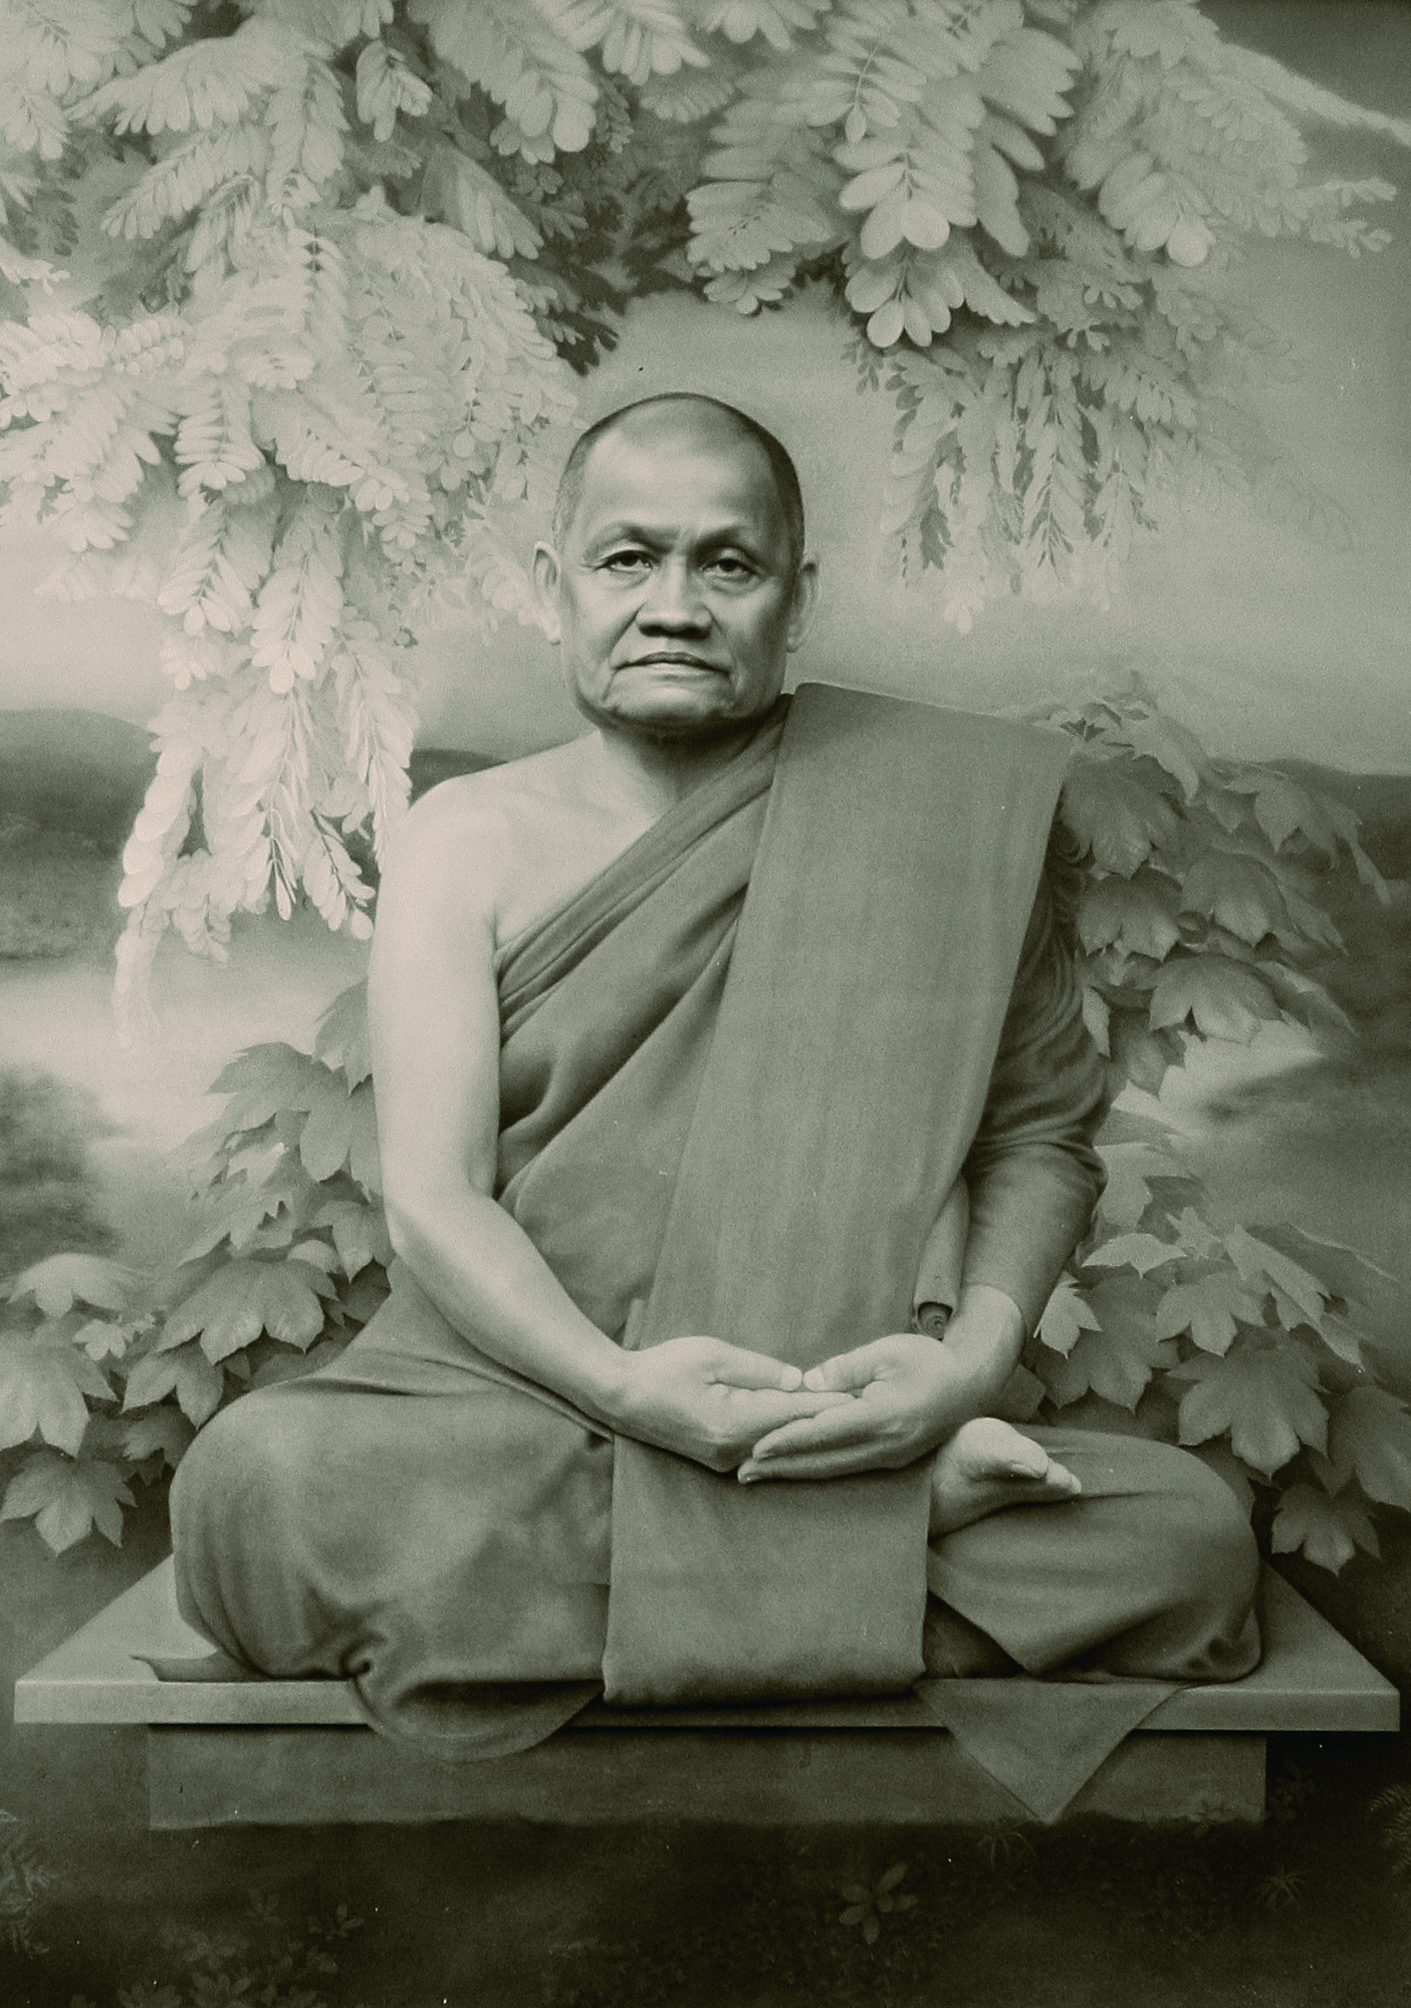
\includegraphics[width=4.5in,keepaspectratio]{Ajahn_Chah_drawing_by_Rollason_CMYK.jpg}%
}}

}



\mbox{}

\cleardoublepage

{\pagestyle{empty}\Large%

{\raggedleft\setlength{\parskip}{0.75em}\setlength{\parindent}{0em}

\vspace*{3\baselineskip}
{\fontGoudy\Large \thetitle}

\vfill

{\Small

Published for free distribution by\\
ARUNA PUBLICATIONS

This book is available for free download at\\
\href{http://www.forestsanghapublications.org/}{www.forestsanghapublications.org}

}

}}

{
\mbox{}\newpage\thispagestyle{empty}%
{\Small\setlength{\parskip}{1em}\setlength{\parindent}{0em}%
{\raggedright%

\thetitle

Published by:

Aruna Publications,\\
Aruna Ratanagiri Buddhist Monastery\\
2 Harnham Hall Cottages,\\
Harnham, Belsay,\\
Northumberland NE20 0HF\\
UK

Contact Aruna Publications at \href{http://aruno.org}{www.aruno.org}\\
This book is available for free download at\\
\href{http://forestsanghapublications.org/}{www.forestsanghapublications.org}

ISBN \theISBN

Copyright \copyright\ 2011 HARNHAM BUDDHIST MONASTERY TRUST

\vfill

{\copyrightsmall

This work is licenced under the Creative Commons Attribution-NonCommercial-NoDerivs 2.0 UK: England \& Wales Licence. To view a copy of this licence, visit:\\
\href{http://creativecommons.org/licenses/by-nc-nd/2.0/uk/}{http://creativecommons.org/licenses/by-nc-nd/2.0/uk/}\\
Or send a letter to: Creative Commons, 444 Castro Street, Suite 900, Mountain View, California, 94041, USA.

See page \pageref{cc-details} for more details on your rights and restrictions under this licence.

Material included in this book has been previously published by Wat Pah Nanachat, Thailand, reprinted here with permission.

Copyright \copyright\ WAT PAH NANACHAT

Design consultant: Neil Taylor.\\ Portrait drawing of Ajahn Chah on page \pageref{aj-chah-portrait} by Gerald~C~Rollason, 1979.

Produced with the {\fontfamily{cms}\selectfont\LaTeX} typesetting system. The body-text is typeset in Gentium, distributed with the SIL Open Font Licence by SIL International.

\theEditionInfo

The Dhamma talk titled `\textit{It Can Be Done}' has been reprinted from
`\textit{Being Dharma}' with permission from Shambhala Publications.

Printed in Malaysia by Bolden Trade.

}

}}

}


\newpage

\vspace*{-2\baselineskip}

{\centering\mbox{}\vspace*{50mm}

\begin{minipage}{0.9\linewidth}\Small\centering\setlength{\parskip}{1em}\setlength{\parindent}{0em}

{\tenandtwelvesize\textit{Gratitude}}
\vspace*{\baselineskip}

This single volume presentation of\\ \textit{The Collected Teachings of Ajahn Chah}\\ is offered as an expression of our deepest gratitude to\\ our teacher, Venerable Ajahn Chah, and to those who have built\\ and maintained his branch monasteries around the world. 

His Sa\.ngha, through the example of their commitment to integrity,\\ contemplation and wisdom, have transformed the lives of millions.\\ The Forest Sa\.ngha communities inspired by Ajahn Chah provide an\\ opportunity for all to practise Dhamma and experience for themselves\\ the wisdom which leads to a life lived in peace and harmony.

\vspace*{2\baselineskip}
The compilers of this volume also wish to acknowledge the support\\ of the many people involved in the preparation of this book --\\ especially to the Kata\~n\~nut\=a group of Malaysia, Singapore and\\ Australia, for bringing it into production.
\bigskip

\end{minipage}

}


\cleartorecto
\tableofcontents

\cleartorecto
\setcounter{page}{1}

% Preface
\input{../.././manuscript/tex/frontmatter_preface_munindo.tex}

% Introduction
\input{../.././manuscript/tex/frontmatter_introduction.volsingle.tex}

% A Note on the Text
\input{../.././manuscript/tex/frontmatter_note-on-the-text.volsingle.tex}


\cleartorecto
\thispagestyle{empty}

{\centering\itshape\mbox{}\vspace*{50mm}

namo tassa bhagavato arahato samm\=asambuddhassa\\
namo tassa bhagavato arahato samm\=asambuddhassa\\
namo tassa bhagavato arahato samm\=asambuddhassa

}


\mainmatter


% The Middle Way Within
\input{../.././manuscript/tex/taste_the-middle-way-within.tex}

% The Peace Beyond
\input{../.././manuscript/tex/taste_the-peace-beyond.tex}

% Convention and Liberation
\input{../.././manuscript/tex/taste_convention-and-liberation.tex}

% No Abiding
\input{../.././manuscript/tex/taste_no-abiding.tex}

% Evening Sitting
% **********************************************************************
% Author: Ajahn Chah
% Translator: 
% Title: Evening Sitting
% First published: The Path to Peace
% Comment: 
% Source: http://ajahnchah.org/ , HTML
% Copyright: Permission granted by Wat Pah Nanachat to reprint for free distribution
% **********************************************************************

\chapter{Evening Sitting}

\index[general]{meditation!general}
\index[general]{confusion}
\index[general]{teachings!understanding}
\vspace*{0.5\baselineskip}
\dropcaps{I}{ would like to ask} you about your practice. You have all been practising meditation here, but are you sure about the practice yet? Ask yourselves, are you confident about the practice yet? These days there are all sorts of meditation teachers around, both monks and lay teachers, and I'm afraid it will cause you to be full of doubts and uncertainty about what you are doing. This is why I am asking. As far as Buddhist practice is concerned, there is really nothing greater or higher than these teachings of the Buddha which you have been practising with here. If you have a clear understanding of them, it will give rise to an absolutely firm and unwavering peace in your heart and mind.

\index[general]{concentration}
\index[general]{mind!nature of}
\index[general]{Noble Eightfold Path}
\index[general]{s\={\i}la, sam\=adhi, pa\~n\~n\=a}
Making the mind peaceful is known as practising meditation, or practising \glsdisp{samadhi}{sam\=adhi.} The mind is something which is extremely changeable and unreliable. Observing from your practice so far, have you seen this yet? Some days you practise sitting meditation and in no time at all the mind is calm, other days you sit and whatever you do there's no calm -- the mind constantly struggles to get away, until it eventually does. Some days it goes well, some days it's awful. This is the way the mind displays these different conditions for you to see. You must understand that the eight factors of the \glsdisp{eightfold-path}{Noble Eightfold Path} merge in \glsdisp{sila}{s\={\i}la,} sam\=adhi and \glsdisp{panna}{pa\~n\~n\=a.} They don't come together anywhere else. This means that when you bring the factors of your practice together, there must be s\={\i}la, there must be sam\=adhi and there must be pa\~n\~n\=a present together in the mind. It means that in practising meditation right here and now, you are creating the causes for the Path to arise in a very direct way.

\index[general]{meditation!instructions}
In sitting meditation you are taught to close your eyes so that you don't spend your time looking at different things. This is because the Buddha was teaching that you should know your own mind. Observe the mind. If you close your eyes, your attention will naturally be turned inwards towards the mind -- the source of many different kinds of knowledge. This is a way of training the mind to give rise to sam\=adhi.

\index[general]{mindfulness of breathing}
\index[general]{mind objects}
\index[general]{path!factors}
Once sitting with the eyes closed, establish awareness with the breath -- make awareness of the breath more important than anything else. This means you bring awareness to follow the breath, and by keeping with it, you will know that place which is the focal point of \glsdisp{sati}{sati,} the focal point of the knowing and the focal point of the mind's awareness. Whenever these factors of the path are working together, you will be able to watch and see your breath, feelings, mind and \pali{\glsdisp{arammana}{\=aramma\d{n}a,}} as they are in the present moment. Ultimately, you will know that place which is both the focal point of sam\=adhi and the unification point of the Path factors.

\index[general]{world!letting go of}
\index[general]{thinking!in meditation}
\index[general]{mind!settling}
When developing sam\=adhi, fix attention on the breath and imagine that you are sitting alone with absolutely no other people and nothing else around to bother you. Develop this perception in the mind, sustaining it until the mind completely lets go of the world outside and all that is left is simply the knowing of the breath entering and leaving. The mind must set aside the external world. Don't allow yourself to start thinking about this person who is sitting over here, or that person who is sitting over there. Don't give space to any thoughts that will give rise to confusion or agitation in the mind -- it's better to throw them out and be done with them. There is no one else here, you are sitting all alone. Develop this perception until all the other memories, perceptions and thoughts concerning other people and things subside, and you're no longer doubting or wondering about the other people or things around you. Then you can fix your attention solely on the in-breaths and out-breaths. Breathe normally. Allow the in-breaths and the out-breaths to continue naturally, without forcing them to be longer or shorter, stronger or weaker than normal. Allow the breath to continue in a state of normality and balance, and then sit and observe it entering and leaving the body.

\index[general]{sound!disturbed by}
Once the mind has let go of external mind-objects, it means you will no longer feel disturbed by the sound of traffic or other noises. You won't feel irritated with anything outside. Whether it's forms, sounds or whatever, they won't be a source of disturbance, because the mind won't be paying attention to them -- it will become centred upon the breath.

If the mind is agitated by different things and you can't concentrate, try taking an extra-deep breath until the lungs are completely full, and then release all the air until there is none left inside. Do this several times, then re-establish awareness and continue to develop concentration. Having re-established mindfulness, it's normal that for a period the mind will be calm, then change and become agitated again. When this happens, make the mind firm, take another deep breath and subsequently expel all the air from your lungs. Fill the lungs to capacity again for a moment and then re-establish mindfulness on the breathing. Fix sati on the in-breaths and the out-breaths, and continue to maintain awareness in this way.

\index[general]{effort!meditation}
The practice tends to be this way, so it will have to take many sittings and much effort before you become proficient. Once you are, the mind will let go of the external world and remain undisturbed. Mind-objects from the outside will be unable to penetrate inside and disturb the mind itself. Once they are unable to penetrate inside, you will see the mind. You will see the mind as one object of awareness, the breath as another and mind-objects as another. They will all be present within the field of awareness, centred at the tip of your nose. Once sati is firmly established with the in-breaths and out-breaths, you can continue to practise at your ease. As the mind becomes calm, the breath, which was originally coarse, becomes correspondingly lighter and more refined. The object of mind also becomes increasingly subtle and refined. The body feels lighter and the mind itself feels progressively lighter and unburdened. The mind lets go of external mind-objects and you continue to observe internally.

\index[general]{awareness!turned inward}
\index[general]{s\={\i}la, sam\=adhi, pa\~n\~n\=a}
\index[general]{mind!one-pointed}
\index[general]{mindfulness of breathing!disappearance of breath}
From here onwards your awareness will be turned away from the world outside and be directed inwards to focus on the mind. Once the mind has gathered together and become concentrated, maintain awareness at that point where the mind becomes focused. As you breathe, you will see the breath clearly as it enters and leaves, sati will be sharp and awareness of mind-objects and mental activity will be clearer. At that point you will see the characteristics of s\={\i}la, sam\=adhi and pa\~n\~n\=a and the way in which they merge together. This is known as the unification of the Path factors. Once this unification occurs, your mind will be free from all forms of agitation and confusion. It will become one-pointed and this is what is known as sam\=adhi.

\looseness=1
When you focus attention in just one place, in this case the breath, you gain a clarity and awareness because of the uninterrupted presence of sati. As you continue to see the breath clearly, sati will become stronger and the mind will become more sensitive in many different ways. You will see the mind in the centre of that place (the breath), one-pointed with awareness focused inwards, rather than turning towards the world outside. The external world gradually disappears from your awareness and the mind no longer goes to perform any work on the outside. It's as if you've come inside your `house', where all your sense faculties have come together to form one compact unit. You are at ease and the mind is free from all external objects. Awareness remains with the breath and over time it will penetrate deeper and deeper inside, becoming progressively more refined.

Ultimately, awareness of the breath becomes so refined that the sensation of the breath seems to disappear. You could say either that awareness of the sensation of the breath has disappeared, or that the breath itself has disappeared. Then there arises a new kind of awareness -- awareness that the breath has disappeared. In other words, awareness of the breath becomes so refined that it's difficult to define it.

\index[general]{knowing!as meditation object}
So it might be that you are just sitting there and there's no breath. Really, the breath is still there, but it has become so refined that it seems to have disappeared. Why? Because the mind is at its most refined, with a special kind of knowing. All that remains is the knowing. Even though the breath has vanished, the mind is still concentrated with the knowledge that the breath is not there. As you continue, what should you take up as the object of meditation? Take this very knowing as the meditation object -- in other words the knowledge that there is no breath -- and sustain this. You could say that a specific kind of knowledge has been established in the mind.

\index[general]{nimittas}
At this point, some people might have doubts arising, because it is here that \pali{\glsdisp{nimitta}{nimitt\=a}} can arise. These can be of many kinds, including both forms and sounds. It is here that all sorts of unexpected things can arise in the course of the practice. If \pali{nimitt\=a} do arise (some people have them, some don't) you must understand them in accordance with the truth. Don't doubt or allow yourself to become alarmed.

\index[general]{concentration!unshakable}
\index[general]{body!disappearance of}
\index[general]{emptiness}
At this stage, you should make the mind unshakeable in its concentration and be especially mindful. Some people become startled when they notice that the breath has disappeared, because they're used to having the breath there. When it appears that the breath has gone, you might panic or become afraid that you are going to die. Here you must establish the understanding that it is just the nature of the practice to progress in this way. What will you observe as the object of meditation now? Observe this feeling that there is no breath and sustain it as the object of awareness as you continue to meditate. The Buddha described this as the firmest, most unshakeable form of sam\=adhi. There is just one firm and unwavering object of mind. When your practice of sam\=adhi reaches this point, there will be many unusual and refined changes and transformations taking place within the mind, of which you can be aware. The sensation of the body will feel at its lightest or might even disappear altogether. You might feel like you are floating in mid-air and seem to be completely weightless. It might be like you are in the middle of space and wherever you direct your sense faculties they don't seem to register anything at all. Even though you know the body is still sitting there, you experience complete emptiness. This feeling of emptiness can be quite strange.

As you continue to practise, understand that there is nothing to worry about. Establish this feeling of being relaxed and unworried, securely in the mind. Once the mind is concentrated and one-pointed, no mind-object will be able to penetrate or disturb it, and you will be able to sit like this for as long as you want. You will be able to sustain concentration without any feelings of pain and discomfort.

\index[general]{concentration!development of}
Having developed sam\=adhi to this level, you will be able to enter or leave it at will. When you do leave it, it's at your ease and convenience. You withdraw at your ease, rather than because you are feeling lazy or tired. You withdraw from sam\=adhi because it is the appropriate time to withdraw, and you come out of it at your will.

\index[general]{concentration}
This is sam\=adhi; you are relaxed and at your ease. You enter and leave it without any problems. The mind and heart are at ease. If you genuinely have sam\=adhi like this, it means that sitting meditation and entering sam\=adhi for just thirty minutes or an hour will enable you to remain cool and peaceful for many days afterwards. Experiencing the effects of sam\=adhi like this for several days has a purifying effect on the mind -- whatever you experience will become an object for contemplation. This is where the practice really begins. It's the fruit which arises as sam\=adhi matures.

\index[general]{s\={\i}la, sam\=adhi, pa\~n\~n\=a}
\index[general]{path}
\index[general]{mind objects}
Sam\=adhi performs the function of calming the mind. Sam\=adhi performs one function, s\={\i}la performs one function and pa\~n\~n\=a performs another function. These characteristics, which you are focusing attention on and developing in the practice are linked, forming a circle. This is the way they manifest in the mind. S\={\i}la, sam\=adhi and pa\~n\~n\=a arise and mature from the same place. Once the mind is calm, it will become progressively more restrained and composed due to the presence of pa\~n\~n\=a and the power of sam\=adhi.

As the mind becomes more composed and refined, this gives rise to an energy which acts to purify s\={\i}la. Greater purity of s\={\i}la facilitates the development of stronger and more refined sam\=adhi, and this in turn supports the maturing of pa\~n\~n\=a. They assist each other in this way. Each aspect of the practice acts as a supporting factor for the other ones -- in the end these terms becoming synonymous. As these three factors continue to mature together, they form one complete circle, ultimately giving rise to \pali{magga}. \pali{Magga} is a synthesis of these three functions of the practice working smoothly and consistently together. As you practise, you have to preserve this energy. It is the energy which will give rise to \glsdisp{vipassana}{vipassan\=a} or pa\~n\~n\=a. Having reached this stage (where pa\~n\~n\=a is already functioning in the mind, independent of whether the mind is peaceful or not), pa\~n\~n\=a will provide a consistent and independent energy in the practice. You see that whenever the mind is not peaceful, you shouldn't attach, and even when it is peaceful, you shouldn't attach. Having let go of the burden of such concerns, the heart will accordingly feel much lighter. Whether you experience pleasant mind-objects or unpleasant mind-objects, you will remain at ease. The mind will remain peaceful in this way.

\index[general]{meditation!after formal practice}
\index[general]{clear comprehension!continuous practice}
Another important thing is to see that when you stop doing formal meditation practice, if there is no wisdom functioning in the mind, you will give up the practice altogether without any further contemplation, development of awareness or thought about the work which still has to be done. In fact, when you withdraw from sam\=adhi, you know clearly in the mind that you have withdrawn. Having withdrawn you should continue to conduct yourself in a normal manner. Maintain mindfulness and awareness at all times. It isn't that you only practise meditation in the sitting posture -- sam\=adhi means the mind which is firm and unwavering. As you go about your daily life, make the mind firm and steady and maintain this sense of steadiness as the object of mind at all times. You must be practising sati and \pali{\glsdisp{sampajanna}{sam\-paja\~n\~na}} continuously.

After you get up from the formal sitting practice and go about your business -- walking, riding in cars and so on -- whenever your eyes see a form or your ears hear a sound, maintain awareness. As you experience mind-objects which give rise to liking and disliking, try to consistently maintain awareness of the fact that such mental states are impermanent and uncertain. In this way the mind will remain calm and in a state of `normality'.

\index[general]{meditation!daily life}
As long as the mind is calm, use it to contemplate mind-objects. Contemplate the whole of this form, the physical body. You can do this at any time and in any posture: whether doing formal meditation practice, relaxing at home, out at work, or in whatever situation you find yourself. Keep the meditation and the reflection going at all times. Just going for a walk and seeing dead leaves on the ground under a tree can provide an opportunity to contemplate impermanence. Both we and the leaves are the same: when we get old, we shrivel up and die. Other people are all the same. This is raising the mind to the level of vipassan\=a, contemplating the truth of the way things are, the whole time. Whether walking, standing, sitting or lying down, sati is sustained evenly and consistently. This is practising meditation correctly -- you have to follow the mind closely, checking it at all times.

Practising here and now at seven o'clock in the evening, we have sat and meditated together for an hour and now stopped. It might be that your mind has stopped practising completely and hasn't continued with the reflection. That's the wrong way to do it. When we stop, all that should stop is the formal meeting and sitting meditation. You should continue practising and developing awareness consistently, without letting up.

\index[general]{practice!consistency}
I've often taught that if you don't practise consistently, it's like drops of water. It's like drops of water because the practice is not a continuous, uninterrupted flow. Sati is not sustained evenly. The important point is that the mind does the practice and nothing else. The body doesn't do it. The mind does the work, the mind does the practice. If you understand this clearly, you will see that you don't necessarily have to do formal sitting meditation in order for the mind to know sam\=adhi. The mind is the one who does the practice. You have to experience and understand this for yourself, in your own mind.

\index[general]{mindfulness}
\index[general]{mind!knowing}
Once you do see this for yourself, you will be developing awareness in the mind at all times and in all postures. If you are maintaining sati as an even and unbroken flow, it's as if the drops of water have joined to form a smooth and continuous flow of running water. Sati is present in the mind from moment to moment and accordingly there will be awareness of mind-objects at all times. If the mind is restrained and composed with uninterrupted sati, you will know mind-objects each time that wholesome and unwholesome mental states arise. You will know the mind that is calm and the mind that is confused and agitated. Wherever you go you will be practising like this. If you train the mind in this way, your meditation will mature quickly and successfully.

\index[general]{insight!retreats}
Please don't misunderstand. These days it's common for people to go on vipassan\=a courses for three or seven days, where they don't have to speak or do anything but meditate. Maybe you have gone on a silent meditation retreat for a week or two, afterwards returning to your normal daily life. You might have left thinking that you've `done vipassan\=a' and, because you feel that you know what it's all about, then carry on going to parties, discos and indulging in different forms of sensual delight. When you do it like this, what happens? There won't be any of the fruits of vipassan\=a left by the end of it. If you go and do all sorts of unskilful things, which disturb and upset the mind, wasting your previous efforts, then next year go back again and do another retreat for seven days or a few weeks, then come out and carry on with the parties, discos and drinking, that isn't true practice. It isn't \pali{\glsdisp{patipada}{pa\d{t}ipad\=a}} or the path to progress.

\index[general]{danger!seeing the}
\index[general]{renunciation}
You need to make an effort to renounce. You must contemplate until you see the harmful effects which come from such behaviour. See the harm in drinking and going out on the town. Reflect and see the harm inherent in all the different kinds of unskilful behaviour which you indulge in, until it becomes fully apparent. This would provide the impetus for you to take a step back and change your ways. Then you would find some real peace. To experience peace of mind you have to clearly see the disadvantages and danger in such forms of behaviour. This is practising in the correct way. If you do a silent retreat for seven days, where you don't have to speak to or get involved with anybody, and then go chatting, gossiping and overindulging for another seven months, how will you gain any real or lasting benefit from those seven days of practice?

\index[general]{practice!consistency}
\index[similes]{spending more than you earn!practice}
I would encourage all the laypeople here who are practising to develop awareness and wisdom to understand this point. Try to practise consistently. See the disadvantages of practising insincerely and inconsistently, and try to sustain a more dedicated and continuous effort in the practice. Just this much. It can then become a realistic possibility that you might put an end to the \pali{\glsdisp{kilesa}{kiles\=a.}} But that lifestyle of not speaking and not playing around for seven days, followed by six months of complete sensual indulgence, without any mindfulness or restraint, will just lead to the squandering of any gains made from the meditation -- there won't be anything left. It's like going to work for a day and earning twenty pounds, but then going out and spending thirty pounds on food and things in the same day; would any money be saved? It would all be gone. It's just the same with the meditation.

This is a form of reminder to you all, so I will ask for your forgiveness. It's necessary to speak in this way, so that those aspects of the practice which are at fault will become clear to you and accordingly, you will be able to give them up. You could say that the reason why you have come to practise is to learn how to avoid doing the wrong things in the future. What happens when you do the wrong things? Doing wrong things leads you to agitation and suffering, when there's no goodness in the mind. It's not the way to peace of mind. This is the way it is. If you practise on a retreat, not talking for seven days, and then go indulging for a few months, no matter how strictly you practised for those seven days, you won't derive any lasting value from that practice. Practising that way, you don't really get anywhere. Many places where meditation is taught don't really get to grips with or get beyond this problem. Really, you have to conduct your daily life in a consistently calm and restrained way.

\index[similes]{planting a tree!practice}
In meditation you have to be constantly turning your attention to the practice. It's like planting a tree. If you plant a tree in one place and after three days pull it up and plant it in a different spot, then after a further three days pull it up and plant it in yet another place, it will just die without producing anything. Practising meditation like this won't bear any fruit either. This is something you have to understand for yourselves. Contemplate it. Try it out for yourselves when you go home. Get a sapling and plant it in one spot, and every few days, go and pull it up and plant it in a different place. It will just die without ever bearing any fruit. It's the same doing a meditation retreat for seven days, followed by seven months of unrestrained behaviour, allowing the mind to become soiled, and then going back to do another retreat for a short period, practising strictly without talking and subsequently coming out and being unrestrained again. As with the tree, the meditation just dies -- none of the wholesome fruits are retained. The tree doesn't grow, the meditation doesn't grow. I say practising this way doesn't bear much fruit.

Actually, I'm not fond of giving talks like this. It's because I feel sorry for you that I have to speak critically. When you are doing the wrong things, it's my duty to tell you, but I'm speaking out of compassion for you. Some people might feel uneasy and think that I'm just scolding them. Really, I'm not just scolding you for its own sake, I'm helping to point out where you are going wrong, so that you know. Some people might think, \pali{\glsdisp{luang-por}{Luang Por}} is just telling us off,' but it's not like that. It's only once in a long while that I'm able to come and give a talk -- if I were to give talks like this every day, you would really get upset! But the truth is, it's not you who gets upset, it's only the \pali{kiles\=a} that are upset. I will say just this much for now. 


% About Being Careful
\input{../.././manuscript/tex/everything_about-being-careful.tex}

% It Can Be Done
\input{../.././manuscript/tex/everything_it-can-be-done.tex}

% Understanding Dukkha
\input{../.././manuscript/tex/everything_undestanding-dukkha.tex}

% The Dhamma Goes Westward
\input{../.././manuscript/tex/everything_dhamma-goes-westward.tex}

% Even One Word Is Enough
\input{../.././manuscript/tex/everything_even-one-word-is-enough.tex}

% Making the Heart Good
\input{../.././manuscript/tex/living_making-the-heart-good.tex}

% Why Are We Here?
\input{../.././manuscript/tex/living_why-are-we-here.tex}

% Our Real Home
\input{../.././manuscript/tex/living_our-real-home.tex}

% The Four Noble Truths
\input{../.././manuscript/tex/living_four-noble-truths.tex}

% Living in the World
% **********************************************************************
% Author: Ajahn Chah
% Translator: 
% Title: Living in the World
% First published: Living Dhamma
% Comment: An informal talk given after an invitation to receive almsfood at a lay person's house in Ubon, the district capital, close to Wat Pah Pong
% Source: http://ajahnchah.org/ , HTML
% Copyright: Permission granted by Wat Pah Nanachat to reprint for free distribution
% **********************************************************************
% Notes on the text: 
% This talk has been published elsewhere under the title `Living in the World with Dhamma'
% **********************************************************************

\chapterFootnote{\textit{Note}: This talk has been published elsewhere under the title: `\textit{Living in the World with Dhamma}'}

\chapter{Living in the World}

\index[general]{practice!real vs. outer}
\index[general]{sense objects!place to practise}
\dropcaps{M}{ost people still don't know} the essence of meditation practice. They think that walking meditation, sitting meditation and listening to Dhamma talks are the practice. These are only the outer forms of practice. The real practice takes place when the mind encounters a sense object. That's the place to practise, where sense contact occurs. When people say things we don't like, there is resentment, if they say things we like, we experience pleasure. Now this is the place to practise. How are we going to practise with these things? This is the crucial point. If we just run around chasing after happiness and running away from suffering all the time, we can practise until the day we die and never see the Dhamma. This is useless. When pleasure and pain arise how are we going to use the Dhamma to be free of them? This is the point of practice.

\index[general]{criticism!how to accept}
Usually when people encounter something disagreeable they don't open up to it. For instance when people are criticized: `Don't bother me! Why blame me?' This is someone who's closed himself off. Right there is the place to practise. When people criticize us we should listen. Are they speaking the truth? We should be open and consider what they are saying. Maybe there is something in what they say, perhaps there is something blameworthy within us. They may be right and yet we immediately take offence. If people point out our faults we should strive to be rid of these faults and improve ourselves. This is how intelligent people practise.

The place where there is confusion is the place where peace can arise. When confusion is penetrated with understanding, what remains is peace. Some people can't accept criticism, they're arrogant. Instead they turn around and argue. This is especially so when adults deal with children. Actually children may say some intelligent things sometimes but if you happen to be their mother, for instance, you can't give in to them. If you are a teacher your students may sometimes tell you something you didn't know, but because you are the teacher you can't listen. This is not right thinking.

\index[general]{S\=ariputta, Ven.}
\index[general]{blind faith}
In the Buddha's time there was one disciple who was very astute. At one time, as the Buddha was expounding the Dhamma, he turned to this monk and asked, `S\=ariputta, do you believe this?' Venerable S\=ariputta replied, `No, I don't yet believe it.' The Buddha praised his answer; `That's very good, S\=ariputta, you are one who is endowed with wisdom. One who is wise doesn't readily believe, he listens with an open mind and then weighs up the truth of that matter before believing or disbelieving.'

\index[general]{authority!questioning}
Now the Buddha here has set a fine example for a teacher. What Venerable S\=ariputta said was true, he simply expressed his true feelings. Some people would think that to say you didn't believe that teaching would be like questioning the teacher's authority, they'd be afraid to say such a thing. They'd just go ahead and agree. This is how the worldly way goes. But the Buddha didn't take offence. He said that you needn't be ashamed of those things which aren't wrong or bad. It's not wrong to say that you don't believe if you don't believe. That's why Venerable S\=ariputta said, `I don't yet believe it.' The Buddha praised him; `This monk has much wisdom. He carefully considers before believing anything.' The Buddha's actions here are a good example for one who is a teacher of others. Sometimes you can learn things even from small children; don't cling blindly to positions of authority.

\index[general]{practice!all postures}
Whether you are standing, sitting, or walking around in various places, you can always study the things around you. We study in the natural way, receptive to all things, be they sights, sounds, smells, tastes, feelings or thoughts. The wise person considers them all. In the real practice, we come to the point where there are no longer any concerns weighing on the mind.

\index[general]{feeling!impermanence of}
If we still don't know like and dislike as they arise, there is still some concern in our minds. If we know the truth of these things, we reflect, `Oh, there is nothing to this feeling of liking here. It's just a feeling that arises and passes away. Dislike is nothing more, just a feeling that arises and passes away. Why make anything out of them?' If we think that pleasure and pain are personal possessions, then we're in for trouble, we never get beyond the point of having some concern or other in an endless chain. This is how things are for most people.

\index[general]{memory!speaking from}
\index[general]{monks!true monk}
\index[general]{Truth!speaking the}
But these days teachers don't often talk about the mind when teaching the Dhamma, they don't talk about the truth. If you talk about the truth people may take exception. They say things like, `He doesn't know time and place, he doesn't know how to speak nicely.' But people should listen to the truth. A true teacher doesn't just talk from memory, he speaks the truth. People in society usually speak from memory, the teacher speaks the truth. People in the society usually speak from memory, and what's more they usually speak in such a way as to exalt themselves. The true monk doesn't speak like that, he speaks the truth, the way things are.

No matter how much the teacher explains the truth, it's difficult for people to understand. It's hard to understand the Dhamma. If you understand the Dhamma you should practise accordingly. It may not be necessary to become a monk, although the monk's life is the ideal form for practice. To really practise, you have to forsake the confusion of the world, give up family and possessions, and take to the forests. These are the ideal places to practise.

\index[general]{practice!as a layperson}
But if we still have family and responsibilities how are we to practise? Some people say it's impossible to practise Dhamma as a layperson. Consider, which group is larger, monks or laypeople? There are far more laypeople. Now if only the monks practise and the laypeople don't, then that means there's going to be a lot of confusion. This is wrong understanding. `I can't become a monk.' Becoming a monk isn't the point! Being a monk doesn't mean anything, if you don't practise. If you really understand the practice of Dhamma then no matter what position or profession you hold in life, be it a teacher, doctor, civil servant or whatever, you can practise the Dhamma every minute of the day.

To think you can't practise as a layman is to lose track of the path completely. Why is it people can find the incentive to do other things? If they feel they are lacking something they make an effort to obtain it. If there is sufficient desire, people can do anything. Some say, `I haven't got time to practise the Dhamma.' I say, `Then how come you've got time to breathe?' Breathing is vital to people's lives. If they saw Dhamma practice as vital to their lives, they would see it as important as their breathing.

\index[general]{practice!how to}
The practice of Dhamma isn't something you have to go running around for or exhaust yourself over. Just look at the feelings which arise in your mind. When the eye sees form, ear hears sounds, nose smells odours and so on, they all come to this one mind, \glsdisp{one-who-knows}{`the one who knows.'} Now when the mind perceives these things what happens? If we like that object we experience pleasure, if we dislike it we experience displeasure. That's all there is to it.

\index[general]{world!knowing the}
So where are you going to find happiness in this world? Do you expect everybody to say only pleasant things to you all your life? Is that possible? No, it's not. If it's not possible, then where are you going to go? The world is simply like this, we must know the world -- \pali{\glsdisp{lokavidu}{lokavid\=u}} -- know the truth of this world. The world is something we should clearly understand. The Buddha lived in this world, he didn't live anywhere else. He experienced family life, but he saw its limitations and detached himself from them. Now, how are you as laypeople going to practise? If you want to practise, you must make an effort to follow the path. If you persevere with the practice, you too will see the limitations of this world and be able to let go.

\index[general]{alcohol!danger of}
People who drink alcohol sometimes say, `I just can't give it up.' Why can't they give it up? Because they don't yet see the liability in it. If they clearly saw the liability in it, they wouldn't have to wait to be told to give it up. If you don't see the liability of something, that means you also can't see the benefit of giving it up. Your practice becomes fruitless, you are just playing at practice. If you clearly see the liability and the benefit of something you won't have to wait for others to tell you about it. 

\index[general]{danger!seeing the}
\index[similes]{eel and snake!seeing the danger}
Consider the story of the fisherman who finds something in his fish-trap. He knows something is in there, he can hear it flapping about inside. Thinking it's a fish, he reaches his hand into the trap, only to find a different kind of animal. He can't yet see it, so he's in two minds about it. It could be an eel\footnote{Considered a delicacy in some parts of Thailand.}, but then again it could be a snake. If he throws it away he may regret it, it could be an eel. On the other hand, if he keeps holding on to it and it turns out to be a snake it may bite him. He's caught in a state of doubt. His desire is so strong he holds on, just in case it's an eel, but the minute he brings it out and sees the striped skin he throws it down straight away. He doesn't have to wait for someone to call out, `It's a snake, it's a snake, let go!' The sight of the snake tells him what to do much more clearly than words could do. Why? Because he sees the danger -- snakes can bite! Nobody has to tell him about it. In the same way, if we practise till we see things as they are, we won't meddle with things that are harmful.

People don't usually practise in this way, they usually do other things. They don't contemplate things, they don't reflect on old age, sickness and death. They only talk about non-ageing and non-death, so they never develop the right feeling for Dhamma practice. They go and listen to Dhamma talks but they don't really listen. Sometimes I get invited to give talks at important functions, but it's a nuisance for me to go. Why so? Because when I look at the people gathered there I can see that they haven't come to listen to the Dhamma. Some are smelling of alcohol, some are smoking cigarettes, some are chatting; they don't look at all like people who have come out of faith in the Dhamma. Giving talks at such places is of little fruit. People who are sunk in heedlessness tend to think things like, `When is he ever going to stop talking? Can't do this, can't do that \ldots{}' Their minds just wander all over the place.

Sometimes they even invite me to give a talk just for the sake of formality: `Please give us just a small Dhamma talk, Venerable Sir.' They don't want me to talk too much, it might annoy them! As soon as I hear people say this I know what they're about. These people don't like listening to Dhamma. It annoys them. If I just give a small talk they won't understand. If you take only a little food, is it enough? Of course not.

\index[similes]{bottle full of water!mind already full}
Sometimes I'm giving a talk, just warming up to the subject, and some drunkard will call out, `Okay, make way, make way for the Venerable Sir, he's coming out now!'--trying to drive me away! If I meet this kind of person I get a lot of food for reflection, I get an insight into human nature. It's like a person having a bottle full of water and then asking for more. There's nowhere to put it. It isn't worth the time and energy to teach them, because their minds are already full. Pour anymore in and it just overflows uselessly. If their bottle was empty, there would be somewhere to put the water, and both the giver and the receiver would benefit.

\index[general]{Dhamma talks!attitude towards}
In this way, when people are really interested in Dhamma and sit quietly, listening carefully, I feel more inspired to teach. If people don't pay attention it's just like the man with the bottle full of water, there's no room to put anymore. It's hardly worth my while talking to them. In situations like this I just don't find any energy arising to teach. You can't put much energy into giving, when no-one's putting much energy into receiving.

These days giving talks tends to be like this, and it's getting worse all the time. People don't search for truth, they study simply to find the necessary knowledge to make a living, raise families and look after themselves. They study for a livelihood. There may be some study of Dhamma, but not much. Students nowadays have much more knowledge than students of previous times. They have all the requisites at their disposal, everything is more convenient. But they also have a lot more confusion and suffering than before. Why is this? Because they only look for the kind of knowledge used to make a living.

\index[general]{practice!vs. study}
Even the monks are like this. Sometimes I hear them say, `I didn't become a monk to practise the Dhamma, I only ordained to study.' These are the words of someone who has completely cut off the path of \mbox{practice.} There's no way ahead, it's a dead end. When these monks teach it's only from memory. They may teach one thing but their minds are in a completely different place. There's no truth in such teachings.

\index[general]{Dhamma!seeing the value in}
This is how the world is. If you try to live simply, practising the Dhamma and living peacefully, they say you are weird and anti-social. They say you're obstructing progress in society. They even intimidate you. Eventually you might even start to believe them and revert to the worldly ways, sinking deeper and deeper into the world until it's impossible to get out. Some people say, `I can't get out now, I've gone in too deeply.' This is how society tends to be. It doesn't appreciate the value of Dhamma.

\index[general]{teaching!the teachings of the Buddha are perfect}
The value of Dhamma isn't to be found in books. Those are just the external appearances of Dhamma, they're not the realization of Dhamma as a personal experience. If you realize the Dhamma, you realize your own mind, you see the truth there. When the truth becomes apparent, it cuts off the stream of delusion.

The teaching of the Buddha is the unchanging truth, whether in the present or in any other time. The Buddha revealed this truth 2,500 years ago and it's been the truth ever since. Nothing should be added to or taken away from it. The Buddha said, `What the \pali{\glsdisp{tathagata}{Tath\=agata}} has laid down should not be discarded, what has not been laid down by the \pali{Tath\=agata} should not be added to the teachings.' He `sealed off' the teachings. Why did the Buddha seal them off? Because these teachings are the words of one who has no defilements. No matter how the world may change, these teachings are unaffected, they don't change with it. If something is wrong, even if people say it's right doesn't make it any the less wrong. If something is right, that doesn't change just because people say it's not. Generation after generation may come and go but these things don't change, because these teachings are the truth.

\index[general]{Truth!constantly true}
Now, who created this truth? The truth itself created the truth! Did the Buddha create it? No, he didn't. The Buddha only \textit{discovered} the truth, the way things are, and then he set out to declare it. The truth is constantly true, whether a Buddha arises in the world or not. The Buddha only `owns' the Dhamma in this sense, he didn't actually create it. It's been here all the time. No-one had previously searched for and found the Deathless then taught it as the Dhamma. But the Buddha didn't invent it, it was already there.

\index[general]{Dhamma!appears and disappears}
At some point in time, the truth is illuminated and the practice of Dhamma flourishes. As time goes on and generations pass away, the practice degenerates until the teaching fades away completely. After a time the teaching is re-founded and flourishes once more. As time goes on the adherents of the Dhamma multiply, prosperity sets in, and once more the teaching begins to follow the darkness of the world. And so once more it degenerates until such a time as it can no longer hold ground. Confusion reigns once more. Then it is time to re-establish the truth. In fact the truth doesn't go anywhere. When Buddhas pass away, the Dhamma doesn't disappear with them.

\index[similes]{mango tree!world cycles}
The world revolves like this. It's something like a mango tree. The tree matures, blossoms, and fruits appear and grow to ripeness. They become rotten and the seed goes back into the ground to become a new mango tree. The cycle starts once more. Eventually there are more ripe fruits which proceed to fall, rot, sink into the ground as seeds and grow once more into trees. This is how the world is. It doesn't go very far, it just revolves around the same old things.

\index[general]{Dhamma!only Dhamma leads to completion}
Our lives these days are the same. Today we are simply doing the same old things we've always done. People think too much. There are so many things to get interested in, but none of them leads to completion. There are the sciences like mathematics, physics, psychology and so on. You can delve into any of these but you can only finalize things with the truth.

\index[similes]{ox pulling a cart!following the world}
Suppose there was a cart being pulled by an ox. As long as the ox pulls the cart the tracks will follow. The wheels are round yet the tracks are long; the tracks are long yet the wheels are merely circles. Just looking at a stationary cart you can't see anything long about it, but once the ox starts moving you see the tracks stretching out behind you. As long as the ox pulls, the wheels keep on turning, but there comes a day when the ox tires and throws off its harness. The ox walks off and leaves the empty cart sitting there. The wheels no longer turn. In time the cart falls apart, its components go back into the four elements -- earth, water, wind and fire.

Searching for peace within the world, the cart wheel tracks stretch out endlessly behind you. As long as you follow the world there is no stopping, no rest. If you simply stop following it, the cart comes to rest, the wheels no longer turn. Following the world turns the wheels ceaselessly. Creating bad \glsdisp{kamma}{kamma} is like this. As long as you follow the old ways, there is no stopping. If you stop, there is stopping. This is how we practise the Dhamma.



% Tuccho Pothila
\input{../.././manuscript/tex/living_tuccho-pothila-venerable-empty-scripture.tex}

% Transcendence
\input{../.././manuscript/tex/food_transcendence.tex}

% Timeless Teachings
% **********************************************************************
% Author: Ajahn Chah
% Translator: 
% Title: Timeless Teachings
% First published: Forest Sa\.ngha Newsletter, January 1997, Number 39
% Comment: 
% Source: 
% Copyright: 
% **********************************************************************

\chapter{Timeless Teachings}

\index[general]{Westerners!attitude of}
\dropcaps{E}{veryone knows suffering} -- but they don't really understand suffering. If we really understood suffering, then that would be the end of our suffering.

Westerners are generally in a hurry, so they have greater extremes of happiness and suffering. The fact that they have much \pali{\glsdisp{kilesa}{kiles\=a,}} can be a source of wisdom later on.

\index[general]{precepts}
To live the lay life and practise Dhamma, one must be in the world but remain above it. \glsdisp{sila}{S\={\i}la,} beginning with the basic \glsdisp{five-precepts}{Five Precepts,} is the all important parent to all good things. It is for removing all wrong from the mind, removing that which causes distress and agitation. When these basic things are gone, the mind will always be in a state of \glsdisp{samadhi}{sam\=adhi.}

\index[general]{morality!make firm}
\index[general]{doubt}
At first, the basic thing is to make s\={\i}la really firm. Practise formal meditation when there is the opportunity. Sometimes it will be good, sometimes not. Don't worry about it, just continue. If doubts arise, just realize that they, like everything else in the mind, are impermanent.

From this base, sam\=adhi will come, but not yet wisdom. One must watch the mind at work -- see like and dislike arising from sense contact, and not attach to them.

\index[similes]{infant crawling!progress in practice}
Don't be anxious for results or quick progress. An infant crawls at first, then learns to walk, then to run and when it is fully grown, can travel half way round the world to Thailand.

\index[general]{generosity!and morality}
\glsdisp{dana}{D\=ana,} if given with good intention, can bring happiness to oneself and others. But until s\={\i}la is complete, giving is not pure, because we may steal from one person and give to another.

\index[similes]{water jar with a hole!seeking pleasure}
Seeking pleasure and having fun is never-ending, one is never satisfied. It's like a water jar with a hole in it. We try to fill it but the water is continually leaking out. The peace of the religious life has a definite end, it puts a stop to the cycle of endless seeking. It's like plugging up the hole in the water jar!

Living in the world, practising meditation, others will look at you like a gong which isn't struck, not producing any sound. They will consider you useless, mad, defeated; but actually it is just the opposite.

\index[general]{teacher!listening to}
As for myself, I never questioned the teachers very much, I have always been a listener. I would listen to what they had to say, whether it was right or wrong did not matter; then I would just practise. The same as you who practise here. You should not have all that many questions. If one has constant mindfulness, then one can examine one's own mental states -- we don't need anyone else to examine our moods.

\index[general]{Chah, Ajahn!early years}
\index[general]{practice!in daily life}
Once when I was staying with an Ajahn I had to sew myself a robe. In those days there weren't any sewing machines, one had to sew by hand, and it was a very trying experience. The cloth was very thick and the needles were dull; one kept stabbing oneself with the needle, one's hands became very sore and blood kept dripping on the cloth. Because the task was so difficult I was anxious to get it done. I became so absorbed in the work that I didn't even notice that I was sitting in the scorching sun dripping with sweat.

The Ajahn came over to me and asked why I was sitting in the sun and not in the cool shade. I told him that I was really anxious to get the work done, `Where are you rushing off to?' He asked. `I want to get this job done so that I can do my sitting and walking meditation.' I told him. `When is our work ever finished?' he asked. `Oh! \ldots{}' This finally brought me around.

`Our worldly work is never finished,' he explained. `You should use such occasions as this as exercises in mindfulness, and then when you have worked long enough just stop. Put it aside and continue your sitting and walking practice.'

\index[general]{effort!in daily activities}
\index[general]{mindfulness!importance of}
\index[general]{mindfulness!daily life}
Now I began to understand his teaching. Previously, when I sewed, my mind also sewed and even when I put the sewing away my mind still kept on sewing. When I understood the Ajahn's teaching I could really put the sewing away. When I sewed, my mind sewed, then when I put the sewing down, my mind put the sewing down also. When I stopped sewing, my mind also stopped sewing.  Know the good and the bad in travelling or in living in one place. You don't find peace on a hill or in a cave; you can travel to the place of the Buddha's enlightenment, without coming any closer to enlightenment. The important thing is to be aware of yourself, wherever you are, whatever you're doing. \pali{\glsdisp{viriya}{Viriya,}} effort, is not a question of what you do outwardly, but just the constant inner awareness and restraint.

\index[general]{fault-finding}
\index[general]{Buddha, the!and his teachers}
It is important not to watch others and find fault with them. If they behave wrongly, there is no need to make yourself suffer. If you point out to them what is correct and they don't practise accordingly, leave it at that. When the Buddha studied with various teachers, he realized that their ways were lacking, but he didn't disparage them. He studied with humility and respect for the teachers, he practised earnestly and realized their systems were not complete, but as he had not yet become enlightened, he did not criticize or attempt to teach them. After he found enlightenment, he recalled those he had studied and practised with and wanted to share his new-found knowledge with them.

We practise to be free of suffering, but to be free of suffering does not mean just to have everything as you would like it, have everyone behave as you would like them to, speaking only that which pleases you. Don't believe your own thinking on these matters. Generally, the truth is one thing, our thinking is another thing. We should have wisdom in excess of thinking, then there is no problem. When thinking exceeds wisdom, we are in trouble.

\index[general]{desire!in practice}
\index[general]{craving!in practice}
\pali{\glsdisp{tanha}{Ta\d{n}h\=a}} in practice can be friend or foe. At first it spurs us to come and practise -- we want to change things, to end suffering. But if we are always desiring something that hasn't yet arisen, if we want things to be other than they are, then this just causes more suffering.

Sometimes we want to force the mind to be quiet, and this effort just makes it all the more disturbed. Then we stop pushing, and sam\=adhi arises; and then in the state of calm and quiet we begin to wonder -- what's going on? What's the point of it? \ldots{} and we're back to agitation again!

\index[general]{Sa\.ngha Council}
\index[general]{\=Ananda, Ven.}
The day before the first \pali{Sa\.nghayana},\footnote{Sa\.ngha Council. The first was convened in the year after the Buddha's final passing away.} one of the Buddha's disciples went to tell \=Ananda: `Tomorrow is the Sa\.ngha council, only \glsdisp{arahant}{arahants} may attend.' \=Ananda was at this time still unenlightened. So he determined: `Tonight I will do it.' He practised strenuously all night, seeking to become enlightened. But he just made himself tired. So he decided to let go, to rest a bit as he wasn't getting anywhere for all his efforts. Having let go, as soon as he lay down and his head hit the pillow, he became enlightened.

\index[general]{suffering!cause of}
\index[general]{sense contact}
\index[general]{birth}
\index[general]{becoming}
\index[general]{sound!disturbed by}
\index[general]{disturbances!by sound}
External conditions don't make you suffer, suffering arises from wrong understanding. Feelings of pleasure and pain, like and dislike, arise from sense-contact -- you must catch them as they arise, not follow them, not giving rise to craving and attachment -- which is in turn causing mental birth and becoming. If you hear people talking, it may stir you up, you think it destroys your calm, your meditation, but you hear a bird chirping and you don't think anything of it, you just let it go as sound, not giving it any meaning or value.

\index[general]{patient endurance!long term view}
\index[general]{people!relating to}
\index[general]{meditation!lost in}
\index[general]{solitude!dangers of}
\index[general]{practice!balancing}
You shouldn't hurry or rush your practice but must think in terms of a long time. Right now we have `new' meditation; if we have `old' meditation, then we can practise in every situation, whether chanting, working, or sitting in your hut. We don't have to go seeking for special places to practise. Wanting to practise alone is half right, but also half wrong. It isn't that I don't favour a lot of formal meditation (sam\=adhi) but one must know when to come out of it. Seven days, two weeks, one month, two months -- and then return to relating to people and situations again. This is where wisdom is gained; too much sam\=adhi practice has no advantage other than that one may become mad. Many monks, wanting to be alone, have gone off and just died alone!

Having the view that formal practice is the complete and only way to practise, disregarding one's normal life situation, is called being intoxicated with meditation.

Meditation is giving rise to wisdom in the mind. This we can do anywhere, any time and in any posture. 


% Fragments of a Teaching
\input{../.././manuscript/tex/bodhinyana_fragments-of-a-teaching.tex}

% A Gift of Dhamma
% **********************************************************************
% Author: Ajahn Chah
% Translator: 
% Title: A Gift of Dhamma
% First published: Bodhinyana
% Comment: A discourse delivered to the assembly of Western monks, novices and lay-disciples at Bung Wai Forest Monastery, Ubon, on the 10th of October, 1977. This discourse was offered to the parents of one of the monks on the occasion of their visit from France.
% Copyright: Permission granted by Wat Pah Nanachat to reprint for free distribution
% **********************************************************************

\chapter{A Gift of Dhamma}

\index[general]{France}
\vspace*{1.5\baselineskip}
 \dropcaps{I}{ am happy that} you have taken this opportunity to come and visit Wat Pah Pong, and to see your son who is a monk here, however I'm sorry I have no gift to offer you. France already has so many material things, but of Dhamma there's very little. Having been there and seen for myself, there isn't really any Dhamma there which could lead to peace and tranquillity. There are only things which continually make one's mind confused and troubled. 

 France is already materially prosperous, it has so many things to offer which are sensually enticing -- sights, sounds, smells, tastes and textures. However, people ignorant of Dhamma only become confused by them. So today I will offer you some Dhamma to take back to France as a gift from Wat Pah Pong and Wat Pah Nanachat. 

\index[general]{Dhamma!what is}
 What is Dhamma? Dhamma is that which can cut through the problems and difficulties of mankind, gradually reducing them to nothing. That's what is called Dhamma and that's what should be studied throughout our daily lives so that when some mental impression arises in us, we'll be able to deal with it and go beyond it. 

\index[general]{problems in life}
 Problems are common to us all whether living here in Thailand or in other countries. If we don't know how to solve them, we'll always be subject to suffering and distress. That which solves problems is wisdom and to have wisdom we must develop and train the mind. 

\index[general]{mind!Thai and Western}
 The subject of practice isn't far away at all, it's right here in our body and mind. Westerners and Thais are the same, they both have a body and mind. A confused body and mind means a confused person and a peaceful body and mind, a peaceful person. 

\index[similes]{putting dye into water!mind}
 Actually, the mind, like rain water, is pure in its natural state. If we were to drop green colouring into clear rain water, however, it would turn green. If we were to drop yellow colouring, it would turn yellow. 

\index[general]{mental impressions}
 The mind reacts similarly. When a comfortable mental impression `drops' into the mind, the mind is comfortable. When the mental impression is uncomfortable, the mind is uncomfortable. The mind becomes `cloudy' just like the coloured water. 

\index[general]{contact}
 When clear water contacts yellow, it turns yellow. When it contacts green, it turns green. It will change colour every time. Actually, that water which is green or yellow is naturally clean and clear. This is also the natural state of the mind, clean and pure and unconfused. It becomes confused only because it pursues mental impressions; it gets lost in its moods! 

\index[similes]{blowing a leaf!mind}
 Let me explain more clearly. Right now we are sitting in a peaceful forest. Here, if there's no wind, a leaf remains still. When a wind blows, it flaps and flutters. The mind is similar to that leaf. When it contacts a mental impression, it, too, `flaps and flutters' according to the nature of that mental impression. And the less we know of Dhamma, the more the mind will continually pursue mental impressions. Feeling happy, it succumbs to happiness. Feeling suffering, it succumbs to suffering. There is constant confusion! 

\index[similes]{child without a mother!mind}
 In the end people become neurotic. Why? Because they don't know! They just follow their moods and don't know how to look after their own minds. When the mind has no one to look after it, it's like a child without a mother or father to take care of it. An orphan has no refuge and, without a refuge, he's very insecure. 

 Likewise, if the mind is not looked after, if there is no training or maturation of character with right understanding, it's really troublesome. 

\index[general]{kamma\d{t}\d{t}h\=ana}
 The method of training the mind which I will give you today is \pali{\glsdisp{kammatthana}{kamma\-\d{t}\d{t}h\=ana.}} \glsdisp{kamma}{Kamma} means `action' and \pali{th\=ana} means `base'. In Buddhism it is the method of making the mind peaceful and tranquil. It's for you to use in training the mind and with the trained mind investigate the body. 

 Our being is composed of two parts: one is the body, the other, the mind. There are only these two parts. What is called `the body' is that which can be seen with our physical eyes. `The mind', on the other hand, has no physical aspect. The mind can only be seen with the `internal eye' or the `eye of the mind'. These two things, body and mind, are in a constant state of turmoil. 

\index[general]{mind!what is the}
 What is the mind? The mind isn't really any `thing'. Conventionally speaking, it's that which feels or senses. That which senses, receives and experiences all mental impressions is called `mind'. Right at this moment there is mind. As I am speaking to you, the mind acknowledges what I am saying. Sounds enter through the ear and you know what is being said. That which experiences this is called `mind'. 

 This mind doesn't have any self or substance. It doesn't have any form. It just experiences mental activities, that's all! If we teach this mind to have \glsdisp{right-view}{right view,} this mind won't have any problems. It will be at ease. 

\index[general]{mind!mental objects}
\index[general]{contact}
 The mind is mind. Mental objects are mental objects. Mental objects are not the mind, the mind is not mental objects. In order to clearly understand our minds and the mental objects in our minds, we say that the mind is that which receives the mental objects which pop into it. When these two things, mind and its object, come into contact with each other, they give rise to feelings. Some are good, some bad, some cold, some hot \ldots{} all kinds! Without wisdom to deal with these feelings, however, the mind will be troubled. 

\index[general]{mindfulness of breathing}
\index[general]{meditation!instructions}
 Meditation is the way of developing the mind so that it may be a base for the arising of wisdom. Here the breath is a physical foundation. We call it \pali{\glsdisp{anapanasati}{\=an\=ap\=anasati}} or `mindfulness of breathing'. Here we make breathing our mental object. We take this object of meditation because it's the simplest and because it has been the heart of meditation since ancient times. 

 When a good occasion arises to do sitting meditation, sit cross-legged: right leg on top of the left leg, right hand on top of the left hand. Keep your back straight and erect. Say to yourself, `Now I will let go of all my burdens and concerns.' You don't want anything that will cause you worry. Let go of all concerns for the time being. 

 Now fix your attention on the breath. Then breathe in and breathe out. In developing awareness of breathing, don't intentionally make the breath long or short. Neither make it strong or weak. Just let it flow normally and naturally. Mindfulness and self-awareness, arising from the mind, will know the in-breath and the out-breath. 

 Be at ease. Don't think about anything. No need to think of this or that. The only thing you have to do is fix your attention on breathing in and breathing out. You have nothing else to do but that! Keep your mindfulness fixed on the in-breath and out-breath as they occur. Be aware of the beginning, middle and end of each breath. On inhalation, the beginning of the breath is at the nose tip, the middle at the heart, and the end in the abdomen. On exhalation, it's just the reverse: the beginning of the breath is in the abdomen, the middle at the heart, and the end at the nose tip. Develop the awareness of the breath: 1, at the nose tip; 2, at the heart; 3, in the abdomen. Then in reverse: 1, in the abdomen; 2, at the heart; 3, at the nose tip. 

 Focusing the attention on these three points will relieve all worries. Just don't think of anything else! Keep your attention on the breath. Perhaps other thoughts will enter the mind, and it will take up other themes and distract you. Don't be concerned. Just take up the breathing again as your object of attention. The mind may get caught up in judging and investigating your moods, but continue to practise, being constantly aware of the beginning, middle and the end of each breath. 

 Eventually, the mind will be aware of the breath at these three points all the time. When you do this practice for some time, the mind and body will get accustomed to the work. Fatigue will disappear. The body will feel lighter and the breath will become more and more refined. Mindfulness and self-awareness will protect the mind and watch over it. 

 We practise like this until the mind is peaceful and calm, until it is one. `One' means that the mind will be completely absorbed in the breathing; that it doesn't separate from the breath. The mind will be unconfused and at ease. It will know the beginning, middle and end of the breath and remain steadily fixed on it. 

 Then, when the mind is peaceful, we fix our attention on the in-breath and out-breath at the nose tip only. We don't have to follow it up and down to the abdomen and back. Just concentrate on the tip of the nose where the breath comes in and goes out. 

\index[general]{mind!calming}
 This is called `calming the mind', making it relaxed and peaceful. When tranquillity arises, the mind stops; it stops with its single object, the breath. This is what's known as making the mind peaceful so that wisdom may arise. 

\index[general]{practice!foundation of}
 This is the beginning, the foundation of our practice. You should try to practise this every single day, wherever you may be. Whether at home, in the car, lying or sitting down, you should be mindfully aware, watching over the mind constantly. 

\index[general]{meditation!all postures}
 This is called mental training and should be practised in all the four postures. Not just sitting, but standing, walking and lying as well. The point is that we should know what the state of the mind is at each moment, and to be able to do this, we must be constantly mindful and aware. Is the mind happy or suffering? Is it confused? Is it peaceful? Getting to know the mind in this manner allows it to become tranquil, and when it does become tranquil, wisdom will arise. 

\index[general]{meditation!body}
\index[general]{meditation!four elements}
 With the tranquil mind, investigate the meditation subject -- the body -- from the top of the head to the soles of the feet, then back to the head. Do this over and over again. Look at and see the hair of the head, hair of the body, the nails, teeth and skin. In this meditation we will see that this whole body is composed of four `elements': earth, water, fire and wind. 

 The hard and solid parts of our body make up the earth element; the liquid and flowing parts, the water element. Winds that pass up and down our body make up the wind element, and the heat in our body, the fire element. 

 Taken together, they compose what we call a `human being'. However, when the body is broken down into its component parts, only these four elements remain. The Buddha taught that there is no `being' per se, no human, no Thai, no Westerner, no person, but that ultimately, there are only these four elements -- that's all! We assume that there is a person or a `being' but, in reality, there isn't anything of the sort. 

\index[general]{three characteristics}
 Whether taken separately as earth, water, fire and wind, or taken together labelling what they form a `human being', they're all impermanent, subject to suffering and not-self. They are all unstable, uncertain and in a state of constant change -- not stable for a single moment!

 Our body is unstable, altering and changing constantly. Hair changes, nails change, teeth change, skin changes -- everything changes, completely! Our mind, too, is always changing. It isn't a self or substance. It isn't really `us', not really `them', although it may think so. Maybe it will think about killing itself. Maybe it will think of happiness or of suffering -- all sorts of things! It's unstable. If we don't have wisdom and we believe this mind of ours, it'll lie to us continually. And alternately we suffer and are happy. 

 This mind is an uncertain thing. This body is uncertain. Together they are impermanent. Together they are a source of suffering. Together they are devoid of self. These, the Buddha pointed out, are neither a being, nor a person, nor a self, nor a soul, nor us, nor them. They are merely elements: earth, water, fire and wind. Elements only! 

 When the mind sees this, it will rid itself of attachment which holds that `I' am beautiful, `I' am good, `I' am evil, `I' am suffering, `I' have, `I' this or `I' that. You will experience a state of unity, for you'll have seen that all of mankind is basically the same. There is no `I'. There are only elements. 

\index[general]{dispassion}
 When you contemplate and see impermanence, suffering and not-self, there will no longer be clinging to a self, a being, I, or he or she. The mind which sees this will give rise to \pali{\glsdisp{nibbida}{nibbid\=a,}} disenchantment and dispassion. It will see all things as only impermanent, suffering and not-self.

 The mind then stops. The mind is Dhamma. Greed, hatred and delusion will then diminish and recede little by little until finally there is only mind -- just the pure mind. This is called `practising meditation'. 

 Thus, I ask you to receive this gift of Dhamma which I offer you to study and contemplate in your daily lives. Please accept this Dhamma teaching from Wat Pah Pong and Wat Pah Nanachat as an inheritance handed down to you. All of the monks here, including your son, and all the teachers, make you an offering of this Dhamma to take back to France with you. It will show you the way to peace of mind, it will render your mind calm and unconfused. Your body may be in turmoil, but your mind will not. Those in the world may be confused, but you will not. Even though there is confusion in your country, you will not be confused because the mind will have seen, the mind is Dhamma. This is the right path, the proper way. 

May you remember this teaching in the future. May you be well and happy.



% Living With the Cobra
\input{../.././manuscript/tex/bodhinyana_living-with-the-cobra.tex}

% Reading the Natural Mind
% **********************************************************************
% Author: Ajahn Chah
% Translator: 
% Title: Reading the Natural Mind
% First published: Bodhinyana
% Comment: An informal talk given to a group of newly ordained monks after the evening chanting, middle of the Rains Retreat, 1978
% Source: http://ajahnchah.org/ , HTML
% Copyright: Permission granted by Wat Pah Nanachat to reprint for free distribution
% **********************************************************************

\chapter{Reading the Natural Mind}

\index[general]{practice!constant}
\dropcaps{O}{ur way of practice} is looking closely at things and making them clear. We're persistent and constant, yet not rushed or hurried. Neither are we too slow. It's a matter of gradually feeling our way and bringing it together. However, all of this bringing together is working towards something, there is a point to our practice. 

For most of us, when we first start to practise, it's nothing other than desire. We start to practise because of wanting. At this stage our wanting is wanting in the wrong way. That is, it's deluded. It's wanting mixed with wrong understanding. 

\index[general]{wisdom}
\index[general]{p\=aram\={\i}}
If wanting is not mixed with wrong understanding like this, we say that it's wanting with wisdom (\glsdisp{panna}{pa\~n\~n\=a}). It's not deluded -- it's wanting with right understanding. In a case like this we say that it's due to a person's \pali{\glsdisp{parami}{p\=aram\={\i}}} or past accumulations. However, this isn't the case with everyone. 

\index[general]{desire!in practice}
Some people don't want to have desire, or they want to not have desires, because they think that our practice is directed at not wanting. However, if there is no desire, then there's no way of practice. 

\index[general]{practice!purpose of}
We can see this for ourselves. The Buddha and all his disciples practised to put an end to defilements. We must want to practise and must want to put an end to defilements. We must want to have peace of mind and want to not have confusion. However, if this wanting is mixed with wrong understanding, then it will only amount to more difficulties for us. If we are honest about it, we really know nothing at all. Or, what we do know is of no consequence, since we are unable to use it properly. 

Everybody, including the Buddha, started out like this, with the desire to practise -- wanting to have peace of mind and wanting to not have confusion and suffering. These two kinds of desire have exactly the same value. If not understood, then both wanting to be free from confusion and not wanting to have suffering are defilements. They're a foolish way of wanting -- desire without wisdom. 

\index[general]{sensuality!sensual indulgence}
\index[general]{self-mortification}
\index[general]{practice!extremes in}
In our practice we see this desire as either sensual indulgence or self-mortification. It's in this very conflict, just this dilemma, that our teacher, the Buddha, was caught up. He followed many ways of practice which merely ended up in these two extremes. And these days we are exactly the same. We are still afflicted by this duality, and because of it we keep falling from the Way. 

\index[general]{craving}
However, this is how we must start out. We start out as worldly beings, as beings with defilements, with wanting devoid of wisdom, desire without right understanding. If we lack proper understanding, then both kinds of desire work against us. Whether it's wanting or not wanting, it's still craving (\pali{\glsdisp{tanha}{ta\d{n}h\=a}}). If we don't understand these two things then we won't know how to deal with them when they arise. We will feel that to go forward is wrong and to go backwards is wrong, and yet we can't stop. Whatever we do we just find more wanting. This is because of the lack of wisdom and because of craving. 

\index[general]{desire!understanding}
It's right here, with this wanting and not wanting, that we can understand the Dhamma. The Dhamma which we are looking for exists right here, but we don't see it. Rather, we persist in our efforts to stop wanting. We want things to be a certain way and not any other way. Or, we want them not to be a certain way, but to be another way. Really these two things are the same. They are part of the same duality. 

\index[general]{Buddha, the!and wanting}
Perhaps we may not realize that the Buddha and all of his disciples had this kind of wanting. However the Buddha understood wanting and not wanting. He understood that they are simply the activity of mind, that such things merely appear in a flash and then disappear. These kinds of desires are going on all the time. When there is wisdom, we don't identify with them -- we are free from clinging. Whether it's wanting or not wanting, we simply see it as such. In reality it's merely the activity of the natural mind. When we take a close look, we see clearly that this is how it is. 

\section*{The Wisdom of Everyday Experience}

\index[similes]{catching a fish!practice}
So it's here that our practice of contemplation will lead us to understanding. Let us take an example, the example of a fisherman pulling in his net with a big fish in it. How do you think he feels about pulling it in? If he's afraid that the fish will escape, he'll be rushed and start to struggle with the net, grabbing and tugging at it. Before he knows it, the big fish has escaped -- he was trying too hard. 

\index[general]{practice!gradual}
In the olden days they would talk like this. They taught that we should do it gradually, carefully gathering it in without losing it. This is how it is in our practice; we gradually feel our way with it, carefully gathering it in without losing it. Sometimes it happens that we don't feel like doing it. Maybe we don't want to look or maybe we don't want to know, but we keep on with it. We continue feeling for it. This is practice: if we feel like doing it, we do it, and if we don't feel like doing it, we do it just the same. We just keep doing it. 

\index[general]{faith!without wisdom}
If we are enthusiastic about our practice, the power of our faith will give energy to what we are doing. But at this stage we are still without wisdom. Even though we are very energetic, we will not derive much benefit from our practice. We may continue with it for a long time and then a feeling arises that we aren't going to find the Way. We may feel that we can not find peace and tranquillity, or that we aren't sufficiently equipped to do the practice. Or maybe we feel that this Way just isn't possible anymore. So we give up! 

\index[general]{patient endurance}
At this point we must be very, very careful. We must use great patience and endurance. It's just like pulling in the big fish -- we gradually feel our way with it. We carefully pull it in. The struggle won't be too difficult, so without stopping we continue pulling it in. Eventually, after some time, the fish becomes tired and stops fighting and we're able to catch it easily. Usually this is how it happens, we practise gradually gathering it together. 

\index[general]{Truth}
\index[general]{experience!wisdom of everyday experience}
It's in this manner that we do our contemplation. If we don't have any particular knowledge or learning in the theoretical aspects of the teachings, we contemplate according to our everyday experience. We use the knowledge which we already have, the knowledge derived from our everyday experience. This kind of knowledge is natural to the mind. Actually, whether we study about it or not, we have the reality of the mind right here already. The mind is the mind whether we have learned about it or not. This is why we say that whether the Buddha is born in the world or not, everything is the way it is. Everything already exists according to its own nature. This natural condition doesn't change, nor does it go anywhere. It just is that way. This is called \pali{\glsdisp{sacca-dhamma}{saccadhamma.}} However, if we don't understand about this \pali{saccadhamma}, we won't be able to recognize it. 

\index[general]{practice!vs. study}
\index[general]{mind!reading the}
So we practise contemplation in this way. If we aren't particularly skilled in scripture, we take the mind itself to study and read. Continually we contemplate,\footnote{Literally: `talk with ourselves'} and understanding regarding the nature of the mind will gradually arise. We don't have to force anything. 

\section*{Constant Effort}

Until we are able to stop our mind, until we reach tranquillity, the mind will just continue as before. It's for this reason that the teacher says, `Just keep on doing it, keep on with the practice!' Maybe we think, `If I don't yet understand, how can I do it?' Until we are able to practise properly, wisdom doesn't arise. So we say just keep on with it. If we practise without stopping, we'll begin to think about what we are doing. We'll start to consider our practice. 

\index[similes]{starting a fire!effort}
\index[general]{effort!constant}
Nothing happens immediately, so in the beginning we can't see any results from our practice. This is like the example I have often given you of the man who tries to make fire by rubbing two sticks of wood together. He says to himself, `They say there's fire here,' and he begins rubbing energetically. He's very impetuous. He rubs on and on but his impatience doesn't end. He keeps wanting to have that fire, but the fire doesn't come. So he stops to rest for a while. He starts again but the going is slow, so he rests again. By then the heat has disappeared; he didn't keep at it long enough. He rubs and rubs until he tires and then he stops altogether. Not only is he tired, but he becomes more and more discouraged until he gives up completely. `There's no fire here!' Actually he was doing the work, but there wasn't enough heat to start a fire. The fire was there all the time but he didn't carry on to the end. 

\index[general]{arahant}
\index[general]{contentment}
\index[general]{confusion}
\index[general]{worldly beings}
This sort of experience causes the meditator to get discouraged in his practice, and so he restlessly changes from one practice to another. And this sort of experience is also similar to our own practice. It's the same for everybody. Why? Because we are still grounded in defilements. The Buddha had defilements also, but he had a lot of wisdom in this respect. While still worldlings the Buddha and the \glsdisp{arahant}{arahants} were just the same as us. If we are still worldlings then we don't think correctly. Thus when wanting arises we don't see it, and when not wanting arises we don't see it. Sometimes we feel stirred up, and sometimes we feel contented. When we have not wanting we have a kind of contentment, but we also have a kind of confusion. When we have wanting, this can be contentment and confusion of another kind. It's all intermixed in this way. 

\section*{Knowing Oneself and Knowing Others}

\index[general]{contemplation!of body parts}
\index[general]{n\=ama-r\=upa!nature of}
The Buddha taught us to contemplate our body, for example: hair of the head, hair of the body, nails, teeth, skin \ldots{} it's all body. Take a look! We are told to investigate right here. If we don't see these things clearly as they are in ourselves, we won't understand regarding other people. We won't see others clearly nor will we see ourselves. However, if we do understand and see clearly the nature of our own bodies, our doubts and wonderings regarding others will disappear. This is because body and mind (\pali{\glsdisp{rupa}{r\=upa}} and \pali{\glsdisp{nama}{n\=ama}}) are the same for everybody. It isn't necessary to go and examine all the bodies in the world since we know that they are the same as us -- we are the same as them. If we have this kind of understanding then our burden becomes lighter. Without this kind of understanding, all we do is develop a heavier burden. In order to know about others, we would have to go and examine everybody in the entire world. That would be very difficult. We would soon become discouraged. 

\index[general]{vinaya}
Our \glsdisp{vinaya}{Vinaya} is similar to this. When we look at our Vinaya we feel that it's very difficult. We must keep every rule, study every rule, review our practice with every rule. If we just think about it, we think `Oh, it's impossible!' We read the literal meaning of all the numerous rules and, if we merely follow our thinking about them, we could well decide that it's beyond our ability to keep them all. Anyone who has had this kind of attitude towards the Vinaya has the same feeling about it -- there are a lot of rules! 

\index[general]{vinaya!how to practise}
The scriptures tell us that we must examine ourselves regarding each and every rule and keep them all strictly. We must know them all and observe them perfectly. This is the same as saying that to understand others we must go and examine absolutely everybody. This is a very heavy attitude. And it's like this because we take what is said literally. If we follow the textbooks, this is the way we must go. Some teachers teach in this manner -- strict adherence to what the textbooks say. It just can't work that way.\footnote{On another occasion the Venerable Ajahn completed the analogy by saying that if we know how to guard our own minds, then it is the same as observing all of the numerous rules of the Vinaya.}

\index[general]{faith}
\index[general]{people!nature of}
Actually, if we study theory like this, our practice won't develop at all. In fact our faith will disappear, our faith in the Way will be destroyed. This is because we haven't yet understood. When there is wisdom we will understand that all the people in the entire world really amount to just this one person. They are the same as this very being. So we study and contemplate our own body and mind. With seeing and understanding the nature of our own body and mind comes the understanding of the bodies and minds of everyone. And so, in this way, the weight of our practice becomes lighter. 

\index[general]{responsibility!for oneself}
The Buddha said we should teach and instruct ourselves -- nobody else can do it for us. When we study and understand the nature of our own existence, we will understand the nature of all existence. Everyone is really the same. We are all the same `make' and come from the same company -- there are only different shades, that's all! Just like \textit{Bort-hai} and \textit{Tum-jai}. They are both pain-killers and do the same thing, but one type is called \textit{Bort-hai} and the other \textit{Tum-jai}. Really they aren't different. 

You will find that this way of seeing things gets easier and easier as you gradually bring it all together. We call this `feeling our way', and this is how we begin to practise. We'll become skilled at doing it. We keep on with it until we arrive at understanding, and when this understanding arises, we will see reality clearly. 
\vspace*{-0.5\baselineskip}

\section*{Theory and Practice}

\vspace*{-0.5\baselineskip}
\index[general]{seven factors of enlightenment}
\index[general]{investigation!of Dhamma}
So we continue this practice until we have a feeling for it. After a time, depending on our own particular tendencies and abilities, a new kind of understanding arises. This we call investigation of Dhamma (\pali{\glsdisp{dhammavicaya}{dhammavicaya}}), and this is how the seven factors of enlightenment arise in the mind. Investigation of Dhamma is one of them. The others are: mindfulness, energy, rapture, tranquillity, concentration (\glsdisp{samadhi}{sam\=adhi}) and equanimity. 

If we have studied about the seven factors of enlightenment, then we'll know what the books say, but we won't have seen the real factors of enlightenment. The real factors of enlightenment arise in the mind. Thus the Buddha came to give us all the various teachings. All the enlightened ones have taught the way out of suffering and their recorded teachings we call the theoretical teachings. This theory originally came from the practice, but it has become merely book learning or words. 

The real factors of enlightenment have disappeared because we don't know them within ourselves, we don't see them within our own minds. If they arise they arise out of practice. If they arise out of practice, then they are factors leading to enlightenment of the Dhamma, and we can use their arising as an indication that our practice is correct. If we are not practising rightly, such things will not appear. 

If we practise in the right way, we can see Dhamma. So we say to keep on practising, feeling your way gradually and continually investigating. Don't think that what you are looking for can be found anywhere other than right here. 

\index[general]{P\=a\d{l}i!learning}
\index[general]{practice!vs. study}
One of my senior disciples had been learning P\=a\d{l}i at a study temple before he came here. He hadn't been very successful with his studies so he thought that, since monks who practise meditation are able to see and understand everything just by sitting, he would come and try this way. He came here to Wat Pah Pong with the intention of sitting in meditation so that he would be able to translate P\=a\d{l}i scriptures. He had this kind of understanding about practice. So I explained to him about our way. He had misunderstood completely. He had thought it an easy matter just to sit and make everything clear. 

\index[general]{investigation!of moods}
If we talk about understanding Dhamma then both study monks and practice monks use the same words. But the actual understanding which comes from studying theory and that which comes from practising\linebreak\ Dhamma is not quite the same. It may seem to be the same, but one is more profound. One is deeper than the other. The kind of understanding which comes from practice leads to surrender, to giving up. Until there is complete surrender we persevere -- we persist in our contemplation. If desires or anger and dislike arise in our mind, we aren't indifferent to them. We don't just leave them, but rather take them and investigate to see how and from where they arise. If such moods are already in our mind, then we contemplate and see how they work against us. We see them clearly and understand the difficulties we cause ourselves by believing and following them. This kind of understanding is not found anywhere other than in our own pure mind. 

\index[similes]{front and back of hand!practice vs. study}
It's because of this that those who study theory and those who practice meditation misunderstand each other. Usually those who emphasize study say things like this, `Monks who only practice meditation just follow their own opinions. They have no basis in the Teaching.' Actually, in one sense, these two ways of study and practice are exactly the same thing. It can help us to understand if we think of it like the front and back of our hand. If we put our hand out, it seems as if the back of the hand has disappeared. Actually the back of our hand hasn't disappeared, it's just hidden underneath. When we say that we can't see it, it doesn't mean that it has disappeared completely, it just means that it's hidden underneath. When we turn our hand over, the same thing happens to the palm of the hand. It doesn't go anywhere, it's merely hidden underneath. 

\index[general]{attachment}
We should keep this in mind when we consider practice. If we think that it has `disappeared', we'll go off to study, hoping to get results. But it doesn't matter how much you study \textit{about} Dhamma, you'll never understand, because you won't know in accordance with truth. If we do understand the real nature of Dhamma, then it becomes letting go. This is surrender -- removing attachment (\pali{\glsdisp{upadana}{up\=ad\=ana}}), not clinging anymore, or, if there still is clinging, it becomes less and less. There is this kind of difference between the two ways of study and practice. 

\index[general]{study!six senses}
\index[general]{six senses}
When we talk about study, we can understand it like this: our eye is a subject of study, our ear is a subject of study -- everything is a subject of study. We can know that form is like this and like that, but we attach to form and don't know the way out. We can distinguish sounds, but then we attach to them. Forms, sounds, smells, tastes, bodily feelings and mental impressions are all like a snare to entrap all beings. 

To investigate these things is our way of practising Dhamma. When some feeling arises, we turn to our understanding to appreciate it. If we are knowledgeable regarding theory, we will immediately turn to that and see how such and such a thing happens like this and then becomes that \ldots{} and so on. If we haven't learned theory in this way, then we have just the natural state of our mind to work with. This is our Dhamma. If we have wisdom then we'll be able to examine this natural mind of ours and use this as our subject of study. It's exactly the same thing. Our natural mind is theory. The Buddha said to take whatever thoughts and feelings arise and investigate them. Use the reality of our natural mind as our theory. We rely on this reality. 

\section*{Insight Meditation (Vipassan\=a)}

\index[general]{mindfulness!at all times}
\index[general]{clear comprehension}
If you have faith it doesn't matter whether you have studied theory or not. If our believing mind leads us to develop practice, if it leads us to constantly develop energy and patience, then study doesn't matter. We have mindfulness as a foundation for our practice. We are mindful in all bodily postures, whether sitting, standing, walking or lying. And if there is mindfulness there will be clear comprehension to accompany it. Mindfulness and clear comprehension will arise together. They may arise so rapidly, however, that we can't tell them apart. But, when there is mindfulness, there will also be clear comprehension. 

\index[general]{three characteristics}
When our mind is firm and stable, mindfulness will arise quickly and easily and this is also where we have wisdom. Sometimes, though, wisdom is insufficient or doesn't arise at the right time. There may be mindfulness and clear comprehension, but these alone are not enough to control the situation. Generally, if mindfulness and clear comprehension are a foundation of mind, then wisdom will be there to assist. However, we must constantly develop this wisdom through the practice of insight meditation. This means that whatever arises in the mind can be the object of mindfulness and clear comprehension. But we must see according to \pali{anicca}, \pali{dukkha}, \pali{anatt\=a}. Impermanence (\pali{anicca}) is the basis. \pali{Dukkha} refers to the quality of unsatisfactoriness, and \pali{anatt\=a} says that it is without individual entity. We see that it's simply a sensation that has arisen, that it has no self, no entity and that it disappears of its own accord. Just that! Someone who is deluded, someone who doesn't have wisdom, will miss this occasion, he won't be able to use these things to his advantage. 

\index[general]{wisdom!and mindfulness}
If wisdom is present then mindfulness and clear comprehension will be right there with it. However, at this initial stage the wisdom may not be perfectly clear. Thus mindfulness and clear comprehension aren't able to catch every object, but wisdom comes to help. It can see what quality of mindfulness is there and what kind of sensation has arisen. Or, in its most general aspect, whatever mindfulness there is or whatever sensation there is, it's all Dhamma. 

\index[general]{meditation!insight}
\index[general]{preferences}
The Buddha took the practice of insight meditation as his foundation. He saw that this mindfulness and clear comprehension were both uncertain and unstable. Anything that's unstable, and which we want to have stable, causes us to suffer. We want things to be according to our own desires, but we suffer because things just aren't that way. This is the influence of an unclean mind, the influence of a mind which is lacking wisdom. 

When we practise we tend to become caught up in wanting it easy, wanting it to be the way we like it. We don't have to go very far to understand such an attitude. Merely look at this body! Is it ever really the way we want it? One minute we like it to be one way and the next minute we like it to be another way. Have we ever really had it the way we liked? The nature of our bodies and minds is exactly the same in this regard. It simply is the way it is. 

This point in our practice can be easily missed. Usually, if whatever we feel doesn't agree with us, we throw out; whatever doesn't please us, we throw out. We don't stop to think whether the way we like and dislike things is really the correct way or not. We merely think that the things we find disagreeable must be wrong, and those which we find agreeable must be right. 

\index[general]{six senses!craving for}
This is where craving comes from. When we receive stimuli by way of eye, ear, nose, tongue, body or mind, a feeling of liking or disliking arises. This shows that the mind is full of attachment. So the Buddha gave us this teaching of impermanence. He gave us a way to contemplate things. If we cling to something which isn't permanent, we'll experience suffering. There's no reason why we should want to have these things in accordance with our likes and dislikes. It isn't possible for us to make things be that way. We don't have that kind of authority or power. Regardless of how we may like things to be, everything is already the way it is. Wanting like this is not the way out of suffering. 

\index[general]{mind!and wisdom}
Here we can see how the mind which is deluded understands in one way, and the mind which is not deluded understands in another way. When the mind with wisdom receives some sensation, for example, it sees it as something not to be clung to or identified with. This is what indicates wisdom. If there isn't any wisdom we merely follow our stupidity. This stupidity is not seeing impermanence, unsatisfactoriness and not-self. That which we like we see as good and right. That which we don't like we see as not good. We can't arrive at Dhamma this way -- wisdom can not arise. If we can see this, then wisdom arises. 

\index[general]{meditation!insight}
\index[general]{three characteristics}
\index[general]{mental impressions}
The Buddha firmly established the practice of insight meditation in his mind and used it to investigate all the various mental impressions. Whatever arose in his mind he investigated like this: even though we like it, it's uncertain. It's suffering, because these things which are constantly rising and falling don't follow the influence of our minds. All these things are not a being or a self, they don't belong to us. The Buddha taught us to see them just as they are. We stand on this principle in our practice. 

\index[general]{moods}
We understand then, that we aren't able to just bring about various moods as we wish. Both good moods and bad moods are going to come up. Some of them are helpful and some of them are not. If we don't understand correctly regarding these things, we won't be able to judge correctly. Rather, we will go running after craving -- running off following our desire. 

Sometimes we feel happy and sometimes we feel sad, but this is natural. Sometimes we'll feel pleased and at other times disappointed. What we like we hold as good, and what we don't like we hold as bad. In this way we separate ourselves further and further from Dhamma. When this happens, we aren't able to understand or recognize Dhamma, and thus we become confused. Desires increase because our minds have nothing but delusion. 

This is how we talk about the mind. It isn't necessary to go far away from ourselves to find understanding. We simply see that these states of mind aren't permanent. We see that they are unsatisfactory and that they aren't a permanent self. If we continue to develop our practice in this way, we call it the practice of \pali{\glsdisp{vipassana}{vipassan\=a}} or insight meditation. We say that it is recognizing the contents of our mind and in this way we develop wisdom. 

\section*{Samatha (Calm) Meditation}

\index[general]{samatha}
\index[general]{meditation!calming}
Our practice of \glsdisp{samatha}{samatha} is like this: we establish the practice of mindfulness on the in-and out-breath, for example, as a foundation or means of controlling the mind. By having the mind follow the flow of the breath it becomes steadfast, calm and still. This practice of calming the mind is called `samatha meditation'. It's necessary to do a lot of this kind of practice because the mind is full of many disturbances. It's very confused. We can't say how many years or how many lives it's been this way. If we sit and contemplate we'll see that there's a lot that doesn't conduce to peace and calm and a lot that leads to confusion! 

\index[general]{meditation!body}
\index[general]{meditation!finding a method}
For this reason the Buddha taught that we must find a meditation subject which is suitable to our particular tendencies, a way of practice which is right for our character. For example, going over and over the parts of the body: hair of the head, hair of the body, nails, teeth and skin, can be very calming. The mind can become very peaceful from this practice. If contemplating these five things leads to calm, it's because they are appropriate objects for contempla\-tion according to our tendencies. Whatever we find to be appropriate in this way, we can consider to be our practice and use it to subdue the defilements. 

\index[general]{death!contemplation of}
Another example is recollection of death. For those who still have strong greed, aversion and delusion and find them difficult to contain, it's useful to take this subject of personal death as a meditation. We'll come to see that everybody has to die, whether rich or poor. We'll see both good and evil people die. Everybody must die! When we develop this practice we find that an attitude of dispassion arises. The more we practise the easier our sitting produces calm. This is because it's a suitable and appropriate practice for us. If this practice of calm meditation is not agreeable to our particular tendencies, it won't produce this attitude of dispassion. If the object is truly suited to us we'll find it arising regularly, without great difficulty, and we'll find ourselves thinking about it often. 

\index[similes]{trays of food!practice}
We can see an example of this in our everyday lives. When laypeople bring trays of many different types of food to offer the monks, we taste them all to see which we like. When we have tried each one, we can tell which is most agreeable to us. This is just an example. That which we find agreeable to our taste we'll eat. We won't bother about the other various dishes. 

\index[general]{mindfulness of breathing}
The practice of concentrating our attention on the in-and out-breath is an example of a type of meditation which is suitable for us all. It seems that when we go around doing various different practices, we don't feel so good. But as soon as we sit and observe our breath we have a good feeling, we can see it clearly. There's no need to go looking far away, we can use what is close to us and this will be better for us. Just watch the breath. It goes out and comes in, out and in -- we watch it like this. For a long time we keep watching our breathing in and out and slowly our mind settles. Other activity will arise but we feel like it is distant from us. Just like when we live apart from each other and don't feel so close anymore. We don't have the same strong contact anymore or perhaps no contact at all. 

\index[general]{death!and mindfulness of breathing}
When we have a feeling for this practice of mindfulness of breathing, it becomes easier. If we keep on with this practice, we gain experience and become skilled at knowing the nature of the breath. We'll know what it's like when it's long and what it's like when it's short. 

We can talk about the food of the breath. While sitting or walking we breathe, while sleeping we breathe, while awake we breathe. If we don't breathe, then we die. If we think about it we see that we exist only with the help of food. If we don't eat ordinary food for ten minutes, an hour or even a day, it doesn't matter. This is a coarse kind of food. However, if we don't breathe for even a short time we'll die. If we don't breathe for five or ten minutes we will be dead. Try it! 

\index[general]{mindfulness of breathing!disappearance of breath}
One who is practising mindfulness of breathing should have this kind of understanding. The knowledge that comes from this practice is indeed wonderful. If we don't contemplate then we won't see the breath as food; but actually we are `eating' air all the time, in, out, in, out \ldots{} all the time. Also you'll find that the more you contemplate in this way, the greater the benefits derived from the practice and the more delicate the breath becomes. It may even happen that the breath stops. It appears as if we aren't breathing at all. Actually, the breath is passing through the pores of the skin. This is called the `delicate breath'. When our mind is perfectly calm, normal breathing can cease in this way. We need not be at all startled or afraid. If there's no breathing what should we do? Just know it! Know that there is no breathing, that's all. This is the right practice here. 

\index[similes]{water urn!practice}
\index[general]{samatha}
Here we are talking about the way of samatha practice, the practice of developing calm. If the object which we are using is right and appropriate for us, it will lead to this kind of experience. This is the beginning, but there is enough in this practice to take us all the way, or at least to where we can see clearly and continue in strong faith. If we keep on with contemplation in this manner, energy will come to us. This is similar to the water in an urn. We put in water and keep it topped up. We keep on filling the urn with water and thereby the insects which live in the water don't die. Making effort and doing our everyday practice is just like this. It all comes back to practice. We feel very good and peaceful. 

\index[similes]{mother and father!meditation}
\index[general]{one-pointedness}
This peacefulness comes from our one-pointed state of mind. This one-pointed state of mind, however, can be very troublesome, since we don't want other mental states to disturb us. Actually, other mental states do come and, if we think about it, that in itself can be the one-pointed state of mind. It's like when we see various men and women, but we don't have the same feeling about them as we do about our mother and father. In reality all men are male just like our father and all women are female just like our mother, but we don't have the same feeling about them. We feel that our parents are more important. They hold greater value for us. 

This is how it should be with our one-pointed state of mind. We should have the same attitude towards it as we would have towards our own mother and father. All other activity which arises we appreciate in the same way as we feel towards men and women in general. We don't stop seeing them, we simply acknowledge their presence and don't ascribe to them the same value as our parents. 

\section*{Undoing the Knot}

\index[general]{samatha}
\index[general]{impermanence}
\index[general]{happiness!impermanence of}
When our practice of samatha arrives at calm, the mind will be clear and bright. The activity of mind will become less and less. The various mental impressions which arise will be fewer. When this happens great peace and happiness will arise, but we may attach to that happiness. We should contemplate that happiness as uncertain. We should also contemplate unhappiness as uncertain and impermanent. We'll understand that all the various feelings are not lasting and therefore not to be clung to. We see things in this way because there's wisdom. We'll understand that things are this way according to their nature. 

\index[similes]{undoing a know!impermanence}
If we have this kind of understanding, it's like taking hold of one strand of a rope which makes up a knot. If we pull it in the right direction, the knot will loosen and begin to untangle. It'll no longer be so tight or so tense. This is similar to understanding that it doesn't always have to be this way. Before, we felt that things would always be the way they were and, in so doing, we pulled the knot tighter and tighter. This tightness is suffering. Living that way is very tense. So we loosen the knot a little and relax. Why do we loosen it? Because it's tight! If we don't cling to it then we can loosen it. It's not a permanent condition that must always be that way. 

\index[general]{understanding!wrong}
We use the teaching of impermanence as our basis. We see that both happiness and unhappiness are not permanent. We see them as not dependable. There is absolutely nothing that's permanent. With this kind of understanding we gradually stop believing in the various moods and feelings which come up in the mind. Wrong understanding will decrease to the same degree that we stop believing in it. This is what is meant by undoing the knot. It continues to become looser. Attachment will be gradually uprooted. 

\section*{Disenchantment}

\index[general]{boredom}
\index[general]{three characteristics}
When we come to see impermanence, unsatisfactoriness and not-self in ourselves, in this body and mind, in this world, then we'll find that a kind of boredom will arise. This isn't the everyday boredom that makes us feel like not wanting to know or see or say anything, or not wanting to have anything to do with anybody at all. That isn't real boredom, it still has attachment, we still don't understand. We still have feelings of envy and resentment and are still clinging to the things which cause us suffering. 

\index[general]{disenchantment}
The kind of boredom which the Buddha talked about is a condition without anger or lust. It arises out of seeing everything as impermanent. When pleasant feeling arises in our mind, we see that it isn't lasting. This is the kind of boredom we have. We call it \pali{\glsdisp{nibbida}{nibbid\=a}} or disenchantment. That means that it's far from sensual craving and passion. We see nothing as being worthy of desire. Whether or not things accord with our likes and dislikes, it doesn't matter to us, we don't identify with them. We don't give them any special value. 

\index[general]{clinging!suffering of}
Practising like this we don't give things reason to cause us difficulty. We have seen suffering and have seen that identifying with moods can not give rise to any real happiness. It causes clinging to happiness and unhappiness and clinging to liking and disliking, which is in itself the cause of suffering. When we are still clinging like this we don't have an even-minded attitude towards things. Some states of mind we like and others we dislike. If we are still liking and disliking, then both happiness and unhappiness are suffering. It's this kind of attachment which causes suffering. The Buddha taught that whatever causes us suffering is in itself unsatisfactory. 

\section*{The Four Noble Truths}

\index[general]{Four Noble Truths!suffering}
Hence we understand that the Buddha's teaching is to know suffering and to know what causes it to arise. And further, we should know freedom from suffering and the way of practice which leads to freedom. He taught us to know just these four things. When we understand these four things we'll be able to recognize suffering when it arises and will know that it has a cause. We'll know that it didn't just drift in! When we wish to be free from this suffering, we'll be able to eliminate its cause. 

Why do we have this feeling of suffering, this feeling of unsatisfactoriness? We'll see that it's because we are clinging to our various likes and dislikes. We come to know that we are suffering because of our own actions. We suffer because we ascribe value to things. So we say, know suffering, know the cause of suffering, know freedom from suffering and know the Way to this freedom. When we know about suffering we keep untangling the knot. But we must be sure to untangle it by pulling in the right \mbox{direction.} That is to say, we must know that this is how things are. Attachment will be torn out. This is the practice which puts an end to our suffering. 

\index[general]{Noble Eightfold Path}
\index[general]{s\={\i}la, sam\=adhi, pa\~n\~n\=a}
\index[general]{suffering!cessation of}
Know suffering, know the cause of suffering, know freedom from suffering and know the path which leads out of suffering. This is \pali{\glsdisp{magga}{magga.}} It goes like this: \glsdisp{right-view}{right view,} right thought, right speech, right action, right livelihood, right effort, right mindfulness, right concentration. When we have the right understanding regarding these things, then we have the path. These things can put an end to suffering. They lead us to morality, concentration and wisdom (\glsdisp{sila}{s\={\i}la,} sam\=adhi, pa\~n\~n\=a). 

\index[general]{Truth}
We must clearly understand these four things. We must want to understand. We must want to see these things in terms of reality. When we see these four things we call this \pali{saccadhamma}. Whether we look inside or in front or to the right or left, all we see is \pali{saccadhamma}. We simply see that everything is the way it is. For someone who has arrived at Dhamma, someone who really understands Dhamma, wherever he goes, everything will be Dhamma. 


% Just Do It!
\input{../.././manuscript/tex/bodhinyana_just-do-it.tex}

% Questions and Answers
\input{../.././manuscript/tex/bodhinyana_questions-and-answers.tex}

% Steady Practice
\input{../.././manuscript/tex/food_right-practice-steady-practice.tex}

% Detachment Within Activity
% **********************************************************************
% Author: Ajahn Chah
% Translator:
% Title: Samma Samadhi -- Detachment Within Activity
% First published: Food for the Heart
% Comment: Given at Wat Pah Pong during the rains retreat, 1977
% Copyright: Permission granted by Wat Pah Nanachat to reprint for free distribution
% **********************************************************************

\chapterFootnote{\textit{Note}: This talk has been published elsewhere under the title: `\textit{Samm\={a} Sam\={a}dhi -- Detachment Within Activity}'}

\chapter{Detachment Within Activity}

\index[general]{Buddha, the!practice}
\dropcaps{T}{ake a look at} the example of the Buddha. Both in his own practice and in his methods for teaching the disciples he was exemplary. The Buddha taught the standards of practice as skilful means for getting rid of conceit. He couldn't do the practice for us. Having heard that teaching, we must further teach ourselves, practise for ourselves. The results will arise here, not at the teaching.

\index[general]{Dhamma!knowing}
The Buddha's teaching can only enable us to get an initial understanding of the Dhamma, but the Dhamma is not yet within our hearts. Why not? Because we haven't yet practised, we haven't yet taught ourselves. The Dhamma arises within the practice. If you know it, you know it through the practice. If you doubt it, you doubt it in the practice. Teachings from the Masters may be true, but simply listening to Dhamma is not yet enough to enable us to realize it. The teaching simply points out the way to realizing the Dhamma. To realize the Dhamma we must take that teaching and bring it into our hearts. That part which is for the body we apply to the body, that part which is for speech we apply to  speech, and that part which is for the mind we apply to the mind. This means that after hearing the teaching we must further teach ourselves to know that Dhamma, to be that Dhamma.

The Buddha said that those who simply believe others are not truly wise. A wise person practises until he is one with the Dhamma, until he can have confidence in himself, independent of others.

\index[general]{S\=ariputta, Ven.}
On one occasion, while Venerable S\=ariputta was sitting at the Buddha's feet, listening respectfully as the Buddha expounded the Dhamma, the Buddha turned to him and asked,

`S\=ariputta, do you believe this teaching?'

Venerable S\=ariputta replied, `No, I don't yet believe it.'

\index[general]{blind faith}
Now this is a good illustration. Venerable S\=ariputta listened, and he took note. When he said he didn't yet believe he wasn't being careless, he was speaking the truth. He simply took note of that teaching, because he had not yet developed his own understanding of it, so he told the Buddha that he didn't yet believe -- because he really didn't believe. These words almost sound as if Venerable S\=ariputta was being rude, but actually he wasn't. He spoke the truth, and the Buddha praised him for it.

`Good, good, S\=ariputta. A wise person doesn't readily believe. He should consider first before believing.'

\index[general]{wrong view}
Conviction in a belief can take various forms. One form reasons according to Dhamma, while another form is contrary to the Dhamma. This second way is heedless, it is a foolhardy understanding, \pali{micch\=a-di\d{t}\d{t}hi}, wrong view. One doesn't listen to anybody else.

\index[general]{D\={\i}ghanakha}
\index[general]{R\=ajagaha}
\index[general]{brahman}
Take the example of D\={\i}ghanakha the \glsdisp{brahman}{Br\=ahman.} This Br\=ahman only believed himself, he wouldn't believe others. At one time when the Buddha was resting at R\=ajagaha, D\={\i}ghanakha went to listen to his teaching. Or you might say that D\={\i}ghanakha went to teach the Buddha because he was intent on expounding his own views.

`I am of the view that nothing suits me.'

This was his view. The Buddha listened to D\={\i}ghanakha's view and then answered,

`Br\=ahman, this view of yours doesn't suit you either.'

When the Buddha had answered in this way, D\={\i}ghanakha was stumped. He didn't know what to say. The Buddha explained in many ways, till the Br\=ahman understood. He stopped to reflect and saw.

`Hmm, this view of mine isn't right.'

On hearing the Buddha's answer the Br\=ahman abandoned his conceited views and immediately saw the truth. He changed right then and there, turning right around, just as one would invert one's hand. He praised the teaching of the Buddha thus:

`Listening to the Blessed One's teaching, my mind was illumined, just as one living in darkness might perceive light. My mind is like an overturned basin which has been uprighted, like a man who has been lost and finds the way.'

\index[general]{right view}
\index[general]{views!and opinions}
\index[general]{Dhamma eye}
Now at that time a certain knowledge arose within his mind, within that mind which had been uprighted. Wrong view vanished and \glsdisp{right-view}{right view} took its place. Darkness disappeared and light arose.

The Buddha declared that the Br\=ahman D\={\i}ghanakha was one who had opened the Dhamma Eye. Previously D\={\i}ghanakha clung to his own views and had no intention of changing them. But when he heard the Buddha's teaching his mind saw the truth, he saw that his clinging to those views was wrong. When the right understanding arose, he was able to perceive his previous understanding as mistaken, so he compared his experience with a person living in darkness who had found light. This is how it is. At that time the Br\=ahman D\={\i}ghanakha transcended his wrong view.

Now we must change in this way. Before we can give up defilements, we must change our perspective. We must begin to practise correctly and practise well. Previously we didn't practise rightly or well, and yet we thought we were right and good just the same. When we really look into the matter we upright ourselves, just like turning over one's hand. This means that the \glsdisp{one-who-knows}{`one who knows',} or wisdom, arises in the mind, so that it is able to see things anew. A new kind of awareness arises.

\index[general]{Buddho!one who knows}
Therefore, practitioners must develop this knowing, which we call \pali{\glsdisp{buddho}{Buddho,}} the one who knows, in their minds. Originally the one who knows is not there, our knowledge is not clear, true or complete. This knowledge is therefore too weak to train the mind. But then the mind changes, or inverts, as a result of this awareness, called `wisdom' or `insight', which exceeds our previous awareness. That previous `one who knows' did not yet know fully and so was unable to bring us to our objective.

\index[general]{opanayiko}
\index[general]{wisdom!arising of}
The Buddha therefore taught to look within, \pali{\glsdisp{opanayiko}{opanayiko.}} Look within, don't look outwards. Or if you look outwards, then look within to see the cause and effect therein. Look for the truth in all things, because external objects and internal objects are always affecting each other. Our practice is to develop a certain type of awareness until it becomes stronger than our previous awareness. This causes wisdom and insight to arise within the mind, enabling us to clearly know the workings of the mind, the language of the mind and the ways and means of all the defilements.

\index[general]{Uddaka R\=amaputta}
\index[general]{concentration!without wisdom}
\index[general]{jh\=ana}
\index[general]{formless absorption}
The Buddha, when he first left his home in search of liberation, was probably not really sure what to do, much like us. He tried many ways to develop his wisdom. He looked for teachers, such as \glsdisp{uddaka-ramaputta}{Uddaka R\=amaputta} to practise meditation -- right leg on left leg, right hand on left hand, body erect, eyes closed, letting go of everything until he was able to attain a high level of absorption (\glsdisp{samadhi}{sam\=adhi}).\footnote{The level of nothingness, one of the `formless absorptions', sometimes called the seventh \pali{\glslink{jhana}{jh\=ana}}, or absorption.} But when he came out of that sam\=adhi his old thinking came up and he would attach to it just as before. Seeing this, he knew that wisdom had not yet arisen. His understanding had not yet penetrated to the truth, it was still incomplete, still lacking. Seeing this he nonetheless gained some understanding -- that this was not yet the summation of practice -- but he left that place to look for a new teacher.

\index[similes]{bee taking nectar!leaving a teacher}
When the Buddha left his old teacher he didn't condemn him, he did as the bee does, it takes nectar from the flower without damaging the petals.

\index[general]{\=Al\=ara K\=al\=ama}
\index[general]{Buddha, the!family of}
\index[general]{R\=ahula, Ven.}
The Buddha then proceeded to study with \glsdisp{alara-kalama}{\=Al\=ara K\=al\=ama} and attained an even higher state of sam\=adhi, but when he came out of that state Bimba and R\=ahula\footnote{Bimba, or Princess Yasodhar\=a, the Buddha's former wife; R\=ahula, his son.} came back into his thoughts again, the old memories and feelings came up again. He still had lust and desire. Reflecting inward he saw that he still hadn't reached his goal, so he left that teacher also. He listened to his teachers and did his best to follow their teachings. He continually reviewed the results of his practice; he didn't simply do things and then discard them for something else.

\index[general]{ascetic practices}
\index[general]{self-mortification}
Then, after trying ascetic practices, he realized that starving until one is almost a skeleton is simply a matter for the body. The body doesn't know anything. Practising in that way was like executing an innocent person while ignoring the real thief.

\index[general]{three characteristics}
When the Buddha really looked into the matter he saw that practise is not a concern of the body, it is a concern of the mind. The Buddha had tried \pali{Attakilamath\=anuyogo} (self-mortification) and found that it was limited to the body. In fact, all Buddhas are enlightened in mind.

\index[general]{self}
\index[general]{not-self}
\index[general]{conditions!arising and ceasing}
Whether in regard to the body or to the mind, just throw them all together as transient, imperfect and ownerless -- \pali{anicca\d{m}} , \pali{dukkha\d{m}}  and \pali{anatt\=a}. They are simply conditions of nature. They arise depending on supporting factors, exist for a while and then cease. When there are appropriate conditions they arise again; having arisen they exist for a while, then cease once more. These things are not a `self', a `being', an `us' or a `them'. There's nobody there, there are simply feelings. Happiness has no intrinsic self, suffering has no intrinsic self. No self can be found, there are simply elements of nature which arise, exist and cease. They go through this constant cycle of change.

\index[general]{clinging}
All beings, including humans, tend to see the arising as themselves, the existence as themselves, and the cessation as themselves. Thus they cling to everything. They don't want things to be the way they are, they don't want them to be otherwise. For instance, having arisen they don't want things to cease; having experienced happiness, they don't want suffering. If suffering does arise they want it to go away as quickly as possible, but it is even better if it doesn't arise at all. This is because they see this body and mind as themselves, or belonging to themselves, and so they demand those things to follow their wishes.

\index[similes]{building a dam!wrong view}
\looseness=1
This sort of thinking is like building a dam or a dyke without making an outlet to let the water through. The result is that the dam bursts. And so it is with this kind of thinking. The Buddha saw that thinking in this way is the cause of suffering. Seeing this cause, the Buddha gave it up.

\index[general]{Four Noble Truths}
\index[general]{n\=ama-r\=upa}
\index[general]{doubt!overcoming}
This is the Noble Truth of the cause of suffering. The truths of suffering, its cause, its cessation and the way leading to that cessation -- people are stuck right here. If people are to overcome their doubts, it's right at this point. Seeing that these things are simply \pali{\glsdisp{rupa}{r\=upa}} and \pali{\glsdisp{nama}{n\=ama,}} or corporeality and mentality, it becomes obvious that they are not a being, a person, an `us', or a `them'. They simply follow the laws of nature.

\index[general]{not-self}
\index[similes]{red hot iron!body and mind}
Our practice is to know things in this way. We don't have the power to really control these things, we aren't really their owners. Trying to control them causes suffering, because they aren't really ours to control. Neither body nor mind are `self' or `other'. If we know this as it really is, then we see clearly. We see the truth, we are at one with it. It's like seeing a lump of red hot iron which has been heated in a furnace. It's hot all over. Whether we touch it on top, the bottom or the sides it's hot. No matter where we touch it, it's hot. This is how you should see things.

\index[general]{practice!doubts}
\index[general]{detachment!how to detach}
Mostly when we start to practise we want to attain, to achieve, to know and to see, but we don't yet know what it is we're going to achieve or know. There was once a disciple of mine whose practice was plagued with confusion and doubts. But he kept practising, and I kept instructing him, till he began to find some peace. But when he eventually became a bit calm he got caught up in his doubts again, saying, `What do I do next?' There! The confusion arises again. He says he wants peace but when he gets it, he doesn't want it, he asks what he should do next!

So in this practice we must do everything with detachment. How are we to detach? We detach by seeing things clearly. Know the characteristics of the body and mind as they are. We meditate in order to find peace, but in doing so we see that which is not peaceful. This is because movement is the nature of the mind.

\index[general]{concentration}
\index[general]{vitakka-vic\=ara}
\index[general]{sensations}
When practising sam\=adhi we fix our attention on the in-breath and out-breath at the nose tip or the upper lip. This `lifting' the mind to fix it is called \pali{\glsdisp{vitakka}{vitakka,}} or `lifting up'. When we have thus `lifted' the mind and are fixed on an object, this is called \pali{\glsdisp{vicara}{vic\=ara,}} the contemplation of the breath at the nose tip. This quality of \pali{vic\=ara} will naturally mingle with other mental sensations, and we may think that our mind is not still, that it won't calm down, but actually this is simply the workings of \pali{vic\=ara} as it mingles with those sensations. Now if this goes too far in the wrong direction, our mind will lose its collectedness. So then we must set up the mind afresh, lifting it up to the object of concentration with \pali{vitakka}. As soon as we have thus established our attention \pali{vic\=ara} takes over, mingling with the various mental sensations.

Now when we see this happening, our lack of understanding may lead us to wonder: `Why has my mind wandered? I wanted it to be still, why isn't it still?' This is practising with attachment.

\index[general]{letting go}
Actually the mind is simply following its nature, but we go and add on to that activity by wanting the mind to be still and thinking, `Why isn't it still?' Aversion arises and so we add that on to everything else, increasing our doubts, increasing our suffering and increasing our confusion. So if there is \pali{vic\=ara}, reflecting on the various happenings within the mind in this way, we should wisely consider, `Ah, the mind is simply like this.' There, that's the one who knows talking, telling you to see things as they are. The mind is simply like this. We let it go at that and the mind becomes peaceful. When it's no longer centred we bring up \pali{vitakka} once more, and shortly there is calm again. \pali{Vitakka} and \pali{vic\=ara} work together like this. We use \pali{vic\=ara} to contemplate the various sensations which arise. When \pali{vic\=ara} becomes gradually more scattered we once again `lift' our attention with \pali{vitakka}.

\index[general]{detachment!within activity}
\index[general]{wrong view}
The important thing here is that our practice at this point must be done with detachment. Seeing the process of \pali{vic\=ara} interacting with the mental sensations we may think that the mind is confused and become averse to this process. This is the cause right here. We aren't happy simply because we want the mind to be still. This is the cause -- wrong view. If we correct our view just a little, seeing this activity as simply the nature of mind, just this is enough to subdue the confusion. This is called letting go.

\index[general]{contemplation}
Now, if we don't attach, if we practise with `letting go' -- detachment within activity and activity within detachment -- if we learn to practise like this, then \pali{vic\=ara} will naturally tend to have less to work with. If our mind ceases to be disturbed, then \pali{vic\=ara} will incline to contemplating Dhamma, because if we don't contemplate Dhamma, the mind returns to distraction.

\index[similes]{flowing water!mind}
So there is \pali{vitakka} then \pali{vic\=ara}, \pali{vitakka} then \pali{vic\=ara}, \pali{vitakka} then \pali{vic\=ara} and so on, until \pali{vic\=ara} becomes gradually more subtle. At first \pali{vic\=ara} goes all over the place. When we understand this as simply the natural activity of the mind, it won't bother us unless we attach to it. It's like flowing water. If we get obsessed with it, asking `Why does it flow?' then naturally we suffer. If we understand that the water simply flows because that's its nature, then there's no suffering. \pali{Vic\=ara} is like this. There is \pali{vitakka}, then \pali{vic\=ara}, interacting with mental sensations. We can take these sensations as our object of meditation, calming the mind by noting those sensations.

\index[general]{rapture}
\index[general]{rapture}
\index[general]{sukha}
\index[general]{one-pointedness}
\index[general]{one-pointedness}
If we know the nature of the mind like this, then we let go, just like letting the water flow by. \pali{Vic\=ara} becomes more and more subtle. Perhaps the mind inclines to contemplating the body, or death for instance, or some other theme of Dhamma. When the theme of contemplation is right, there will arise a feeling of well-being. What is that well-being? It is \pali{\glsdisp{piti}{p\={\i}ti}} (rapture). \pali{P\={\i}ti}, well-being, arises. It may manifest as goose-pimples, coolness or lightness. The mind is enrapt. This is called \pali{p\={\i}ti}. There is also pleasure, \pali{\glsdisp{sukha}{sukha,}} the coming and going of various sensations; and the state of \pali{\glsdisp{ekaggata}{ekaggat\=aramma\d{n}a,}} or one-pointedness.

\index[general]{jh\=ana!factors of}
\index[general]{jh\=ana!1st-4th}
Now if we talk in terms of the first stage of concentration, it must be like this: \pali{vitakka}, \pali{vic\=ara}, \pali{p\={\i}ti}, \pali{sukha}, \pali{ekaggat\=a}. So what is the second stage like? As the mind becomes progressively more subtle, \pali{vitakka} and \pali{vic\=ara} become comparatively coarser, so that they are discarded, leaving only \pali{p\={\i}ti}, \pali{sukha}, and \pali{ekaggat\=a}. This is something that the mind does of itself, we don't have to conjecture about it, we just know things as they are.

As the mind becomes more refined, \pali{p\={\i}ti} is eventually thrown off, leaving only \pali{sukha} and \pali{ekaggat\=a}, and so we take note of that. Where does \pali{p\={\i}ti} go to? It doesn't go anywhere, it's just that the mind becomes increasingly more subtle so that it throws off those qualities that are too coarse for it. Whatever is too coarse it throws out, and it keeps throwing off like this until it reaches the peak of subtlety, known in the books as the fourth \pali{jh\=ana}, the highest level of absorption. Here the mind has progressively discarded whatever becomes too coarse for it, until only \pali{ekaggat\=a} and \pali{\glsdisp{upekkha}{upekkh\=a,}} equanimity remain. There's nothing further, this is the limit.

\index[general]{practice!desire for results}
\index[general]{craving}
\index[general]{vitakka-vic\=ara}
When the mind is developing the stages of sam\=adhi it must proceed in this way, but please let us understand the basics of practice. We want to make the mind still but it won't be still. This is practising out of desire, but we don't realize it. We have the desire for calm. The mind is already disturbed and then we further disturb things by wanting to make it calm. This very wanting is the cause. We don't see that this wanting to calm the mind is \pali{\glsdisp{tanha}{ta\d{n}h\=a.}} It's just like increasing the burden. The more we desire calm the more disturbed the mind becomes, until we just give up. We end up fighting all the time, sitting and struggling with ourselves.

\index[general]{mind!nature of}
\index[general]{sensations!contemplation of}
Why is this? Because we don't reflect back on how we have set up the mind. Know that the conditions of mind are simply the way they are. Whatever arises, just observe it. It is simply the nature of the mind; it isn't harmful unless we don't understand its nature. It's not dangerous if we see its activity for what it is. So we practise with \pali{vitakka} and \pali{vic\=ara} until the mind begins to settle down and becomes less forceful. When sensations arise we contemplate them, we mingle with them and come to know them.

However, usually we tend to start fighting with them, because right from the beginning we're determined to calm the mind. As soon as we sit, the thoughts come to bother us. As soon as we set up our meditation object our attention wanders, the mind wanders off following all the thoughts, thinking that those thoughts have come to disturb us, but actually the problem arises right here, from the very wanting to calm the mind.

\index[similes]{talking children!mind}
If we see that the mind is simply behaving according to its nature, that it naturally comes and goes like this, and if we don't get over-interested in it, we can understand that its ways are much the same as a child. Children don't know any better, they may say all kinds of things. If we understand them we just let them talk, because children naturally talk like that. When we let go like this, we are not obsessed with the child. We can talk to our guests undisturbed, while the child chatters and plays around. The mind is like this. It's not harmful unless we grab on to it and get obsessed over it. That's the real cause of trouble.

\index[general]{rapture}
\index[similes]{fruit in a bowl!absorption}
When \pali{p\={\i}ti} arises one feels an indescribable pleasure, which only those who experience it can appreciate. \pali{Sukha} (pleasure) arises, and there is also the quality of one-pointedness. There is \pali{vitakka}, \pali{vic\=ara}, \pali{p\={\i}ti}, \pali{sukha} and \pali{ekaggat\=a}. These five qualities all converge at one place. Even though they are different qualities they are all collected in one place, and we can see them all there, just like seeing many different kinds of fruit in one bowl. \pali{Vitakka}, \pali{vic\=ara}, \pali{p\={\i}ti}, \pali{sukha} and \pali{ekaggat\=a} -- we can see them all in one mind, all five qualities. If one were to ask, `How is there \pali{vitakka}, how is there \pali{vic\=ara}, how is there \pali{p\={\i}ti} and \pali{sukha}? 'It would be difficult to answer, but when they converge in the mind we will see how it is for ourselves.

\index[general]{clear comprehension}
\index[general]{not-self}
At this point our practice becomes somewhat special. We must have recollection and self-awareness and not lose ourselves. Know things for what they are. These are stages of meditation, the potential of the mind. Don't doubt anything with regard to the practice. Even if you sink into the earth or fly into the air, or even `die' while sitting, don't doubt it. Whatever the qualities of the mind are, just stay with the knowing. This is our foundation: to have \glsdisp{sati}{sati,} recollection, and \pali{\glsdisp{sampajanna}{sampaja\~n\~na,}} self-awareness, whether standing, walking, sitting, or reclining. Whatever arises, just leave it be, don't cling to it. Whether it's like or dislike, happiness or suffering, doubt or certainty, contemplate with \pali{vic\=ara} and gauge the results of those qualities. Don't try to label everything, just know it. See that all the things that arise in the mind are simply sensations. They are transient. They arise, exist and cease. That's all there is to them, they have no self or being, they are neither `us' nor `them'. None of them are worthy of clinging to.

\index[general]{n\=ama-r\=upa}
\index[general]{impermanence}
\index[general]{disenchantment}
When we see all \pali{r\=upa} and \pali{n\=ama} in this way with wisdom, then we will see the old tracks. We will see the transience of the mind, the transience of the body, the transience of happiness, suffering, love and hate. They are all impermanent. Seeing this, the mind becomes weary; weary of the body and mind, weary of the things that arise and cease and their transience. When the mind becomes disenchanted it will look for a way out of all those things. It no longer wants to be stuck in things, it sees the inadequacy of this world and the inadequacy of birth.

\index[general]{three characteristics}
When the mind sees like this, wherever we go, we see \pali{anicca\d{m}} (transience), \pali{dukkha\d{m}} (imperfection) and \pali{anatt\=a} (ownerlessness). There's nothing left to hold on to. Whether we sit at the foot of a tree, on a mountain top or in a valley, we can hear the Buddha's teaching. All trees will seem as one, all beings will be as one, there's nothing special about any of them. They arise, exist for a while, age and then die, all of them.

We thus see the world more clearly, we see this body and mind more clearly. They are clearer in the light of transience, clearer in the light of imperfection and clearer in the light of ownerlessness. If people hold fast to things, they suffer. This is how suffering arises. If we see that body and mind are simply the way they are, no suffering arises, because we don't hold fast to them. Wherever we go we will have wisdom. Even when seeing a tree we can consider it with wisdom. Seeing grass and the various insects will be food for reflection.

\index[general]{Dhamma!true Dhamma}
When it all comes down to it, they all fall into the same boat. They are all Dhamma, they are invariably transient. This is the truth, this is the true Dhamma, this is certain. How is it certain? It is certain in that the world is that way and can never be otherwise. There's nothing more to it than this. If we can see in this way, we have finished our journey.

\index[general]{conceit}
In Buddhism, with regard to view, it is said that to feel that we are more foolish than others is not right; to feel that we are equal to others is not right; and to feel that we are better than others is not right, because there isn't any `we'. This is how it is, we must uproot conceit.

\index[general]{knower of the world}
\index[general]{world!knowing the}
This is called \pali{\glsdisp{lokavidu}{lokavid\=u}} -- knowing the world clearly as it is. If we thus see the truth, the mind will know itself completely and will sever the cause of suffering. When there is no longer any cause, the results can not arise. This is the way our practice should proceed.

\index[general]{carelessness}
\index[general]{practice!basics}
The basics which we need to develop are: firstly, to be upright and honest; secondly, to be wary of wrongdoing; thirdly, to have the attribute of humility within our heart, to be aloof and content with little. If we are content with little in regards to speech and all other things, we will see ourselves, we won't be drawn into distractions. The mind will have a foundation of \glsdisp{sila}{s\={\i}la,} sam\=adhi, and \glsdisp{panna}{pa\~n\~n\=a.}

Therefore, practitioners of the path should not be careless. Even if you are right, don't be careless. And if you are wrong, don't be careless. If things are going well or you're feeling happy, don't be careless. Why do I say `don't be careless'? Because all of these things are uncertain. Note them as such. If you get peaceful just leave the peace be. You may really want to indulge in it but you should simply know the truth of it, the same as for unpleasant qualities.

This practice of the mind is up to each individual. The teacher only explains the way to train the mind, because that mind is within each individual. We know what's in there, nobody else can know our mind as well as we can. The practice requires this kind of honesty. Do it properly, don't do it half-heartedly. When I say `do it properly,' does that mean you have to exhaust yourselves? No, you don't have to exhaust yourselves, because the practice is done in the mind. If you know this, you will know the practice. You don't need a whole lot. Just use the standards of practice to reflect on yourself inwardly.

\index[general]{determination}
Now the Rains Retreat is half way over. For most people it's normal to let the practice slacken off after a while. They aren't consistent from beginning to end. This shows that their practice is not yet mature. For instance, having determined a particular practice at the beginning of the retreat, whatever it may be, then we must fulfil that resolution. For these three months make the practice consistent. You must all try. Whatever you have determined to practise, consider that and reflect whether the practice has slackened off. If so, make an effort to re-establish it. Keep shaping up the practice, just the same as when we practise meditation on the breath. As the breath goes in and out the mind gets distracted. Then re-establish your attention on the breath. When your attention wanders off again bring it back once more. This is the same. In regard to both the body and the mind the practice proceeds like this. Please make an effort with it.



% Training this Mind
% **********************************************************************
% Author: Ajahn Chah
% Translator: 
% Title: Training this Mind
% First published: Taste of Freedom
% Comment: 
% Source: http://ajahnchah.org/ , HTML
% Copyright: Permission granted by Wat Pah Nanachat to reprint for free distribution
% **********************************************************************
% Notes on the text:
% This talk was previously printed as a different translation under the title `About this Mind'
% **********************************************************************

\renewcommand{\chapterFootnotemark}{\footnotemark}
\renewcommand{\chapterFootnotetext}{\footnotetext{\textit{Note}: A different translation of this talk has been published elsewhere under the title: `\textit{About This Mind}'}}

\chapter{Training this Mind}

\index[general]{mind!training}
\index[general]{moods!following}
\dropcaps{T}{raining this mind} -- actually there's nothing much to this mind. It's simply radiant in and of itself. It's naturally peaceful. Why the mind doesn't feel peaceful right now is because it gets lost in its own moods. There's nothing to the mind itself. It simply abides in its natural state, that's all. That sometimes the mind feels peaceful and other times not peaceful is because it has been tricked by these moods. The untrained mind lacks wisdom. It's foolish. Moods come and trick it into feeling pleasure one minute and suffering the next. Happiness then sadness. But the natural state of a person's mind isn't one of happiness or sadness. This experience of happiness and sadness is not the actual mind itself, but just these moods which have tricked it. The mind gets lost, carried away by these moods with no idea what's happening. And as a result, we experience pleasure and pain accordingly, because the mind has not been trained yet. It still isn't very clever. And we go on thinking that it's our mind which is suffering or our mind which is happy, when actually it's just lost in its various moods. 

\index[general]{pleasure and pain}
\index[general]{feeling}
\index[general]{thinking!nature of}
\index[general]{mind!peace}
The point is that really this mind of ours is naturally peaceful. It's still and calm like a leaf that is not being blown about by the wind. But if the wind blows, then it flutters. It does that because of the wind. And so with the mind it's because of these moods -- getting caught up with thoughts. If the mind didn't get lost in these moods, it wouldn't flutter about. If it understood the nature of thoughts, it would just stay still. This is called the natural state of the mind. And why we have come to practise now is to see the mind in this original state. We think that the mind itself is actually pleasurable or peaceful. But really the mind has not created any real pleasure or pain. These thoughts have come and tricked it and it has got caught up in them. So we really have to come and train our minds in order to grow in wisdom. So that we understand the true nature of thoughts rather than just following them blindly.

The mind is naturally peaceful. It's in order to understand just this much that we have come together to do this difficult practice of meditation.



% Tranquillity and Insight
% **********************************************************************
% Author: Ajahn Chah
% Translator: 
% Title: On Meditation
% First published: Taste of Freedom
% Comment: An informal talk given in the Northeastern dialect, taken from an unidentified tape
% Source: http://ajahnchah.org/ , HTML
% Copyright: Permission granted by Wat Pah Nanachat to reprint for free distribution
% **********************************************************************

\chapterFootnote{\textit{Note}: This talk has been published elsewhere under the title: `\textit{On Meditation}'}

\chapter{Tranquillity and Insight}

\index[general]{meditation}
\index[general]{mind!strengthening}
\dropcaps{T}{o calm the mind} means to find the right balance. If you try to force your mind too much it goes too far; if you don't try enough it doesn't get there, it misses the point of balance. 

\index[general]{concentration}
Normally the mind isn't still, it's moving all the time. We must make an effort to strengthen the mind. Making the mind strong and making the body strong are not the same. To make the body strong we have to exercise it, to push it, but to make the mind strong means to make it peaceful, not to go thinking of this and that. For most of us the mind has never been peaceful, it has never had the energy of \glsdisp{samadhi}{sam\=adhi;} so we must establish it within a boundary. We sit in meditation, staying with the \glsdisp{one-who-knows}{`one who knows'.} 

\index[similes]{sowing machine!meditation}
\index[general]{mindfulness of breathing}
If we force our breath to be too long or too short, we're not balanced, the mind won't become peaceful. It's like when we first start to use a pedal sewing machine. At first we just practise pedalling the machine to get our coordination right, before we actually sew anything. Following the breath is similar. We don't get concerned over how long or short, weak or strong it is, we just note it. We simply let it be, following the natural breathing. 

\looseness=-1
When our breathing is balanced, we take it as our meditation object. When we breathe in, the beginning of the breath is at the nose tip, the middle of the breath at the chest and the end of the breath at the abdomen. This is the path of the breath. When we breathe out, the beginning of the breath is at the abdomen, the middle at the chest and the end at the nose-tip. Simply take note of this path of the breath at the nose tip, the chest and the abdomen, then at the abdomen, the chest and the tip of the nose. We take note of these three points in order to make the mind firm, to limit mental activity so that mindfulness and self-awareness can easily arise. 

When our attention settles on these three points, we can let them go and note the in and out breathing, concentrating solely at the nose tip or the upper lip, where the air passes on its in and out passage. We don't have to follow the breath, we just establish mindfulness in front of us at the nose tip, and note the breath at this one point -- entering, leaving, entering, leaving. 

There's no need to think of anything special, just concentrate on this simple task for now, having continuous presence of mind. There's nothing more to do, just breath in and out. Soon the mind becomes peaceful, the breath refined. The mind and body become light. This is the right state for the work of meditation. 

\index[general]{vitakka-vic\=ara}
\index[general]{self-awareness}
When sitting in meditation the mind becomes refined, but we should try to be aware, to know whatever state it's in. Mental activity is there together with tranquillity. There is \pali{\glsdisp{vitakka}{vitakka.}} \pali{Vitakka} is the action of bringing the mind to the theme of contemplation. If there is not much mindfulness, there will not be much \pali{vitakka}. Then \pali{\glsdisp{vicara}{vic\=ara,}} the contemplation around that theme, follows. Various weak mental impressions may arise from time to time but our self-awareness is the important thing -- whatever may be happening we know it continuously. As we go deeper we are constantly aware of the state of our meditation, knowing whether or not the mind is firmly established. Thus, both concentration and awareness are present. 

\index[general]{mental impressions}
\index[general]{jh\=ana!factors of}
\index[general]{one-pointedness}
Having a peaceful mind does not mean that there's nothing happening, mental impressions do arise. For instance, when we talk about the first level of absorption, we say it has five factors. Along with \pali{vitakka} and \pali{vic\=ara}, \pali{\glsdisp{piti}{p\={\i}ti}}  arises with the theme of contemplation and then \pali{\glsdisp{sukha}{sukha.}} These four things all lie together in the mind that is established in tranquillity. They are as one state. 

\index[general]{jh\=ana!description}
The fifth factor is \pali{\glsdisp{ekaggata}{ekaggat\=a}} or one-pointedness. You may wonder how there can be one-pointedness when there are all these other factors as well. This is because they all become unified on that foundation of tranquillity. Together they are called a state of sam\=adhi. They are not everyday states of mind, they are factors of absorption. There are these five characteristics, but they do not disturb the basic tranquillity. There is \pali{vitakka}, but it does not disturb the mind; \pali{vic\=ara}, rapture and happiness arise but do not disturb the mind. The mind is therefore as one with these factors. The first level of absorption is like this. 

We don't have to call it first \pali{\glsdisp{jhana}{jh\=ana,}} second \pali{jh\=ana}, third \pali{jh\=ana} and so on, let's just call it `a peaceful mind'. As the mind becomes progressively calmer it will dispense with \pali{vitakka} and \pali{vic\=ara}, leaving only rapture and happiness. Why does the mind discard \pali{vitakka} and \pali{vic\=ara}? This is because, as the mind becomes more refined, the activities of \pali{vitakka} and \pali{vic\=ara} are too coarse to remain. At this stage, as the mind leaves off \pali{vitakka} and \pali{vic\=ara}, feelings of great rapture can arise, tears may gush out. But as the sam\=adhi deepens, rapture too is discarded, leaving only happiness and one-pointedness, until finally even happiness goes and the mind reaches its greatest refinement. There is only equanimity and one-pointedness, all else has been left behind. The mind stands unmoving. 

\index[general]{mind!peace}
\index[general]{hindrances}
Once the mind is peaceful this can happen. You don't have to think a lot about it; it just happens by itself when the causal factors are ripe. This is called the energy of a peaceful mind. In this state the mind is not drowsy; the five hindrances (sense desire, aversion, restlessness, dullness and doubt) have all fled. 

But if mental energy is still not strong and mindfulness is weak, there will occasionally arise intruding mental impressions. The mind is peaceful but it's as if there's a `cloudiness' within the calm. It's not a normal sort of drowsiness though, some impressions will manifest -- maybe we'll hear a sound or see a dog or something. It's not really clear but it's not a dream either. This is because these five factors have become unbalanced and weak. 

\index[general]{doubt}
\index[similes]{moon covered by clouds!meditation}
The mind tends to play tricks within these levels of tranquillity. `Im\-agery' will sometimes arise when the mind is in this state, through any of the senses, and the meditator may not be able to tell exactly what is happening. `Am I sleeping? No. Is it a dream? No, it's not a dream.' These impressions arise from a middling sort of tranquillity; but if the mind is truly calm and clear we don't doubt the various mental impressions or imagery which arise. Questions like, `Did I drift off then? Was I sleeping? Did I get lost?' don't arise, for they are characteristics of a mind which is still doubting. `Am I asleep or awake?' Here, the mind is fuzzy. This is the mind getting lost in its moods. It's like the moon going behind a cloud. You can still see the moon but the clouds covering it render it hazy. It's not like the moon which has emerged from behind the clouds clear, sharp and bright. 

When the mind is peaceful and established firmly in mindfulness and self-awareness, there will be no doubt concerning the various phenomena which we encounter. The mind will truly be beyond the hindrances. We will clearly know everything which arises in the mind as it is. We do not doubt because the mind is clear and bright. The mind which reaches sam\=adhi is like this.

\index[general]{concentration}
Some people find it hard to enter sam\=adhi because they don't have the right tendencies. There is sam\=adhi, but it's not strong or firm. However, one can attain peace through the use of wisdom, through contemplating and seeing the truth of things, solving problems that way. This is using wisdom rather than the power of sam\=adhi. To attain calm in practice, it's not necessary to be sitting in meditation. For instance, just ask yourself, `Eh, what is that?' and solve your problem right there! A person with wisdom is like this. Perhaps he can't really attain high levels of sam\=adhi, although there must be some concentration, just enough to cultivate wisdom. It's like the difference between farming rice and farming corn. One can depend on rice more than corn for one's livelihood. Our practice can be like this, we depend more on wisdom to solve problems. When we see the truth, peace arises. 

\index[general]{practice!character types}
\index[general]{concentration}
The two ways are not the same. Some people have insight and are strong in wisdom but do not have much sam\=adhi. When they sit in meditation they aren't very peaceful. They tend to think a lot, contemplating this and that, until eventually they contemplate happiness and suffering and see the truth of them. Some incline more towards this than sam\=adhi. Whether standing, walking, sitting or lying, enlightenment of the Dhamma can take place. Through seeing, through relinquishing, they attain peace. They attain peace through knowing the truth, through going beyond doubt, because they have seen it for themselves. 

\index[general]{right view}
Other people have only little wisdom but their sam\=adhi is very strong. They can enter very deep sam\=adhi quickly, but not having much wisdom, they can not catch their defilements; they don't know them. They can't solve their problems. But regardless of whichever approach we use, we must do away with wrong thinking, leaving only \glsdisp{right-view}{right view.} We must get rid of confusion, leaving only peace. Either way we end up at the same place. There are these two sides to practice, but these two things, calm and insight, go together. We can't do away with either of them. They must go together. 

\index[general]{mindfulness!importance of}
That which `looks over' the various factors which arise in meditation is \glsdisp{sati}{sati,} mindfulness. This sati is a condition which, through practise, can help other factors to arise. Sati is life. Whenever we don't have sati, when we are heedless, it's as if we are dead. If we have no sati, then our speech and actions have no meaning. Sati is simply recollection. It's a cause for the arising of self-awareness and wisdom. Whatever virtues we have cultivated are imperfect if lacking in sati. Sati is that which watches over us while standing, walking, sitting and lying. Even when we are no longer in sam\=adhi, sati should be present throughout. 

\index[general]{shame!sense of}
Whatever we do, we take care. A sense of shame\footnote{This is a wholesome sense of shame based on knowledge of cause and effect, rather than emotional guilt.} will arise. We will feel ashamed about the things we do which aren't correct. As shame increases, our collectedness will increase as well. When collectedness increases, heedlessness will disappear. Even if we don't sit in meditation, these factors will be present in the mind. 

And this arises because of cultivating sati. Develop sati! This is the quality which looks over the work we are doing in the present. It has real value. We should know ourselves at all times. If we know ourselves like this, right will distinguish itself from wrong, the path will become clear, and the cause for all shame will dissolve. Wisdom will arise. 

\index[general]{s\={\i}la, sam\=adhi, pa\~n\~n\=a}
We can bring the practice all together as morality, concentration and wisdom. To be collected, to be controlled, this is morality. The firm establishing of the mind within that control is concentration. Complete, overall knowledge within the activity in which we are engaged is wisdom. The practice in brief is just morality, concentration and wisdom, or in other words, the path. There is no other way.


% The Path in Harmony
% **********************************************************************
% Author: Ajahn Chah
% Translator: 
% Title: The Path in Harmony
% First published: Taste of Freedom
% Comment: A composite of two talks given in England in 1979 and 1977 respectively
% Copyright: Permission granted by Wat Pah Nanachat to reprint for free distribution
% **********************************************************************

\chapter{The Path in Harmony}

\index[general]{uncertainty}
\vspace*{0.5\baselineskip}
\dropcaps{T}{oday I would like} to ask you all: `are you sure yet, are you certain in your meditation practice?' I ask because these days there are many people teaching meditation, both monks and laypeople, and I'm afraid you may be subject to wavering and doubt. If we understand clearly, we will be able to make the mind peaceful and firm. 

\index[general]{Noble Eightfold Path}
You should understand the \glsdisp{eightfold-path}{eightfold path} as morality, concentration and wisdom. The path comes together as simply this. Our practice is to make this path arise within us. 

\index[general]{meditation!instructions}
When sitting in meditation we are told to close our eyes, not to look at anything else, because now we are going to look directly at the mind. When we close our eyes, our attention comes inwards. We establish our attention on the breath, centre our feelings there, put our mindfulness there. When the factors of the path are in harmony we will be able to see the breath, the feelings, the mind and mental objects for what they are. Here we will see the `focus point', where \glsdisp{samadhi}{sam\=adhi} and the other factors of the path converge in harmony. 

When we are sitting in meditation, following the breath, think to yourself that now you are sitting alone. There is no one sitting around you, there is nothing at all. Develop this feeling that you are sitting alone until the mind lets go of all externals, concentrating solely on the breath. If you are thinking, `This person is sitting over here, that person is sitting over there,' there is no peace, the mind doesn't come inwards. Just cast all that aside until you feel there is no one sitting around you, until there is nothing at all, until you have no wavering or interest in your surroundings. 

Let the breath go naturally, don't force it to be short or long or whatever, just sit and watch it going in and out. When the mind lets go of all external impressions, the sounds of cars and such will not disturb you. Nothing, whether sights or sounds, will disturb you, because the mind doesn't receive them. Your attention will come together on the breath. 

If the mind is confused and won't concentrate on the breath, take a full, deep breath, as deep as you can, and then let it all out till there is none left. Do this three times and then re-establish your attention. The mind will become calm. 

\index[general]{mindfulness of breathing}
It's natural for it to be calm for a while, and then restlessness and confusion may arise again. When this happens, concentrate, breathe deeply again, and then re-establish your attention on the breath. Just keep going like this. When this has happened many times you will become adept at it. The mind will let go of all external manifestations. External impressions will not reach the mind. \glsdisp{sati}{Sati} will be firmly established. 

\index[general]{s\={\i}la, sam\=adhi, pa\~n\~n\=a}
As the mind becomes more refined, so does the breath. Feelings will become finer and finer, the body and mind will be light. Our attention is solely on the inner, we see the in-breaths and out-breaths clearly, we see all impressions clearly. Here we will see the coming together of morality, concentration and wisdom. This is called the path in harmony. When there is this harmony our mind will be free of confusion, it will come together as one. This is called sam\=adhi. 

\index[general]{mindfulness of breathing!disappearance of breath}
After watching the breath for a long time, it may become very refined; the awareness of the breath will gradually cease, leaving only bare awareness. The breath may become so refined it disappears! Perhaps we are `just sitting', as if there is no breathing at all. Actually there is breathing, but it seems as if there's none. This is because the mind has reached its most refined state, there is just bare awareness. It has gone beyond the breath. The knowledge that the breath has disappeared becomes established. What will we take as our object of meditation now? We take just this knowledge as our object, that is, the awareness that there's no breath. 

Unexpected things may happen at this time; some people experience them, some don't. If they do arise, we should be firm and have strong mindfulness. Some people see that the breath has disappeared and get a fright, they're afraid they might die. Here we should know the situation just as it is. We simply notice that there's no breath and take that as our object of awareness. 

This, we can say, is the firmest, surest type of sam\=adhi: there is only one firm, unmoving state of mind. Perhaps the body will become so light it's as if there is no body at all. We feel like we're sitting in empty space, completely empty. Although this may seem very unusual, you should understand that there's nothing to worry about. Firmly establish your mind like this. 

\index[general]{mind!unification}
When the mind is firmly unified, having no sense impressions to disturb it, one can remain in that state for any length of time. There will be no painful feelings to disturb us. When sam\=adhi has reached this level, we can leave it when we choose, but if we come out of this sam\=adhi, we do so comfortably, not because we've become bored with it or tired. We come out because we've had enough for now, we feel at ease; we have no problems at all. 

\index[general]{concentration!fruit of}
If we can develop this type of sam\=adhi, then if we sit, say, thirty minutes or an hour, the mind will be cool and calm for many days. When the mind is cool and calm like this, it is clean. Whatever we experience, the mind will take up and investigate. This is a fruit of sam\=adhi. 

\index[general]{s\={\i}la, sam\=adhi, pa\~n\~n\=a}
Morality has one function, concentration has another function and wisdom another. These factors are like a cycle. We can see them all within the peaceful mind. When the mind is calm it has collectedness and restraint because of wisdom and the energy of concentration. As it becomes more collected it becomes more refined, which in turn gives morality the strength to increase in purity. As our morality becomes purer, this will help in the development of concentration. When concentration is firmly established it helps in the arising of wisdom. Morality, concentration and wisdom help each other, they are interrelated like this. 

In the end the path becomes one and functions at all times. We should look after the strength which arises from the path, because it is the strength which leads to insight and wisdom. 

\section{On the Dangers Of Sam\=adhi}

\index[general]{concentration!dangers of}
Sam\=adhi is capable of bringing much harm or much benefit to the meditator. You can't say it brings only one or the other. For one who has no wisdom it is harmful, but for one who has wisdom it can bring real benefit, it can lead to insight. 

\index[general]{jh\=ana}
\index[general]{happiness}
That which can possibly be harmful to the meditator is absorption sam\=adhi (\pali{\glsdisp{jhana}{jh\=ana}}), the sam\=adhi with deep, sustained calm. This sam\=adhi brings great peace. Where there is peace, there is happiness. When there is happiness, attachment and clinging to that happiness arise. The meditator doesn't want to contemplate anything else, he just wants to indulge in that pleasant feeling. When we have been practising for a long time we may become adept at entering this sam\=adhi very quickly. As soon as we start to note our meditation object, the mind enters calm, and we don't want to come out to investigate anything. We just get stuck on that happiness. This is a danger to one who is practising meditation. 

\index[general]{concentration!upac\=ara-sam\=adhi}
\index[general]{sense impressions}
\index[general]{thinking}
\index[general]{awareness!and calm}
We must use \pali{\glsdisp{upacara-samadhi}{upac\=ara-sam\=adhi:}} Here, we enter calm and then, when the mind is sufficiently calm, we come out and look at outer activity.\footnote{`Outer activity' refers to all manner of sense impressions. It is used in contrast to the `inner inactivity' of absorption sam\=adhi (\pali{jh\=ana}), where the mind does not `go out' to external sense impressions.} Looking at the outside with a calm mind gives rise to wisdom. This is hard to understand, because it's almost like ordinary thinking and imagining. When thinking is there, we may think the mind isn't peaceful, but actually that thinking is taking place within the calm. There is contemplation but it doesn't disturb the calm. We may bring thinking up in order to contemplate it. Here we take up thinking to investigate it, it's not that we are aimlessly thinking or guessing away; it's something that arises from a peaceful mind. This is called `awareness within calm and calm within awareness'. If it's simply ordinary thinking and imagining, the mind won't be peaceful, it will be disturbed. But I am not talking about ordinary thinking; this is a feeling that arises from the peaceful mind. It's called `contemplation'. Wisdom is born right here. 

\index[general]{concentration!right}
\index[general]{concentration!wrong}
\index[similes]{sharp knife!concentration}
So, there can be right sam\=adhi and wrong sam\=adhi. Wrong sam\=adhi is where the mind enters calm and there's no awareness at all. One could sit for two hours or even all day but the mind doesn't know where it's been or what's happened. It doesn't know anything. There is calm, but that's all. It's like a well-sharpened knife which we don't bother to put to any use. This is a deluded type of calm, because there is not much self-awareness. The meditator may think he has reached the ultimate already, so he doesn't bother to look for anything else. Sam\=adhi can be an enemy at this level. Wisdom can not arise because there is no awareness of right and wrong. 

With right sam\=adhi, no matter what level of calm is reached, there is awareness. There is full mindfulness and clear comprehension. This is the sam\=adhi which can give rise to wisdom, one can not get lost in it. Practitioners should understand this well. You can't do without this awareness, it must be present from beginning to end. This kind of sam\=adhi has no danger. 

\index[general]{wisdom!and concentration}
You may wonder: where does the benefit arise, how does the wisdom arise, from sam\=adhi? When right sam\=adhi has been developed, wisdom has the chance to arise at all times. When the eye sees form, the ear hears sound, the nose smells odours, the tongue experiences taste, the body experiences touch or the mind experiences mental impressions -- in all postures -- the mind stays with full knowledge of the true nature of those sense impressions, it doesn't follow them. 

\index[general]{practice!right practice}
\index[general]{mindfulness!all postures}
\index[general]{happiness}
When the mind has wisdom it doesn't `pick and choose'. In any posture we are fully aware of the birth of happiness and unhappiness. We let go of both of these things, we don't cling. This is called right practice, which is present in all postures. These words `all postures' do not refer only to bodily postures, they refer to the mind, which has mindfulness and clear comprehension of the truth at all times. When sam\=adhi has been rightly developed, wisdom arises like this. This is called `insight', knowledge of the truth. 

\index[general]{becoming}
\index[general]{birth}
\index[general]{clinging}
\index[general]{sa\d{m}s\=ara}
There are two kinds of peace -- the coarse and the refined. The peace which comes from sam\=adhi is the coarse type. When the mind is peaceful there is happiness. The mind then takes this happiness to be peace. But happiness and unhappiness are becoming and birth. There is no escape from \glsdisp{samsara}{sa\d{m}s\=ara} here because we still cling to them. So happiness is not peace, peace is not happiness. 

The other type of peace is that which comes from wisdom. Here we don't confuse peace with happiness; we know the mind which contemplates and knows happiness and unhappiness as peace. The peace which arises from wisdom is not happiness, but is that which sees the truth of both happiness and unhappiness. Clinging to those states does not arise, the mind rises above them. This is the true goal of all Buddhist practice. 


% The Place of Coolness
\input{../.././manuscript/tex/taste_right-view-the-place-of-coolness.tex}

% Monastery of Confusion
% **********************************************************************
% Author: Ajahn Chah
% Translator: 
% Title: Monastery of Confusion
% First published: Everything is Teaching Us
% Comment: 
% Source: http://ajahnchah.org/ , HTML
% Copyright: Permission granted by Wat Pah Nanachat to reprint for free distribution
% **********************************************************************
% Notes on the text: 
% A large section of this Dhamma talk has previously been published under the title `Free From Doubt'
% **********************************************************************

\renewcommand{\chapterFootnotemark}{\footnotemark}
\renewcommand{\chapterFootnotetext}{\footnotetext{\textit{Note}: This talk has been published elsewhere under the title: `\textit{Free From Doubt}'}}

\chapter{Monastery of Confusion}

\index[general]{monks!attitude towards laypeople}
\index[general]{laypeople}
\vspace*{\baselineskip}
\dropcaps{S}{taying or going is not important,} but our thinking is. So all of you, please work together, cooperate and live in harmony. This should be the legacy you create here at Wat Pah Nanachat Bung Wai, the International Forest Monastery of Bung Wai District. Don't let it become Wat Pah Nanachat \textit{Woon Wai}, the International Forest Monastery of Confusion and Trouble.\footnote{One of Ajahn Chah's favourite plays on words.} Whoever comes to stay here should be helping create this legacy. 

The way I see it, the laypeople are providing robes material, almsfood, the dwelling place, and medicines in appropriate measure. It's true that they are simple country folk, but they support you out of their faith as best they can. Don't get carried away with your ideas of how you think they should be, such as, `Oh, I try to teach these laypeople, but they do make me upset. Today is the observance day, and they came to take precepts. Then tomorrow they'll go casting their fishing nets. They'll drink their whisky. They do these things right out there where anyone can see. Then the next observance day, they'll come again. They'll take the precepts and listen to the Dhamma talk again, and then they'll go to put out their nets again, kill animals again, and drink again.'

You can get pretty upset thinking like this. You'll think that your activities with the laypeople don't bring any benefit at all. Today they take the precepts, and tomorrow they go cast fishing nets. A monk without much wisdom might get discouraged and feel he's failed, thinking his work bears no fruit. But it's not that his efforts have no result; it's those laypeople who get no result. Of course there is some good result from making efforts at virtue. So when there is such a situation and we start to suffer over it, what should we do?

\index[general]{perseverance}
We contemplate within ourselves to recognize that our good intentions have brought some benefit and do have meaning. It's just that the spiritual faculties of those people aren't developed. They aren't strong yet. That's how it is for now, so we patiently continue to advise them. If we just give up on such people, they are likely to become worse than they are now. If we keep at it, they may come to maturity one day and recognize their unskilful actions. Then they will feel some remorse and start to be ashamed of doing such things.

\index[general]{generosity!virtues of}
\looseness=1
Right now, they have the faith to support us with material offerings, giving us our requisites for living. I've considered this; it's quite a big deal. It's no small thing. Donating our food, our dwellings, the medicines to treat our illnesses, is not a small thing. We are practising for the attainment of \glsdisp{nibbana}{Nibb\=ana.} If we don't have any food to eat, that will be pretty difficult. How would we sit in meditation? How would we be able to build this monastery?

\index[similes]{buying/selling medicine!attitude towards laity}
We should recognize when people's spiritual faculties are not yet mature. So what should we do? We are like someone selling medicine. You've probably seen or heard them driving around with their loudspeakers touting the different medicines they have for different maladies. People who have bad headaches or poor digestion might come to buy.

We can accept money from those who buy our medicine; we don't take money from someone who doesn't buy anything. We can feel glad about the people who do buy something. If others stay in their houses and don't come out to buy, we shouldn't get angry with them for that. We shouldn't criticize them.

\index[general]{teaching!laypeople}
If we teach people but they can't practise properly, we shouldn't be getting angry with them. Don't do that! Don't criticize them, but rather keep on instructing them and leading them along. Whenever their faculties have ripened sufficiently, then they will want to do it. Just like when we are selling medicine, we just keep on doing our business. When people have ailments that trouble them, they will buy. Those who don't see a need to buy medicine probably aren't suffering from any such conditions. So never mind. 

Keeping at it with this attitude, these problems will be done with. There were such situations in the Buddha's time too. 

\index[general]{p\=aram\={\i}}
\index[similes]{ripening fruit!p\=aram\={\i}}
We want to do it right, but somehow we can't get there yet; our own faculties are not sufficiently mature. Our \pali{\glsdisp{parami}{p\=aram\={\i}}} are not complete. It's like fruit that's still growing on the tree. You can't force it to be sweet -- it's still unripe, it's small and sour, simply because it hasn't finished growing. You can't force it to be bigger, to be sweet, to be ripe -- you have to let it ripen according to its nature. As time passes and things change, people may come to spiritual maturity. As time passes the fruit will grow, ripen and sweeten of its own accord. With such an attitude you can be at ease. But if you are impatient and dissatisfied, you keep asking, `Why isn't this mango sweet yet? Why is it sour?' It's still sour because it's not ripe. That's the nature of fruit. 

\index[similes]{four kinds of lotus!people in the world}
The people in the world are like that. It makes me think of the Buddha's teaching about four kinds of lotus. Some are still in the mud, some have grown out of the mud but are under the water, some are at the surface of the water, and some have risen above the water and blossomed. The Buddha was able to give his teachings to so many various beings because he understood their different levels of spiritual development. We should think about this and not feel oppressed by what happens here. Just consider yourselves to be like someone selling medicine. Your responsibility is to advertise it and make it available. If someone gets sick, they are likely to come and buy it. Likewise, if people's spiritual faculties mature sufficiently, one day they are likely to develop faith. It's not something we can force them to do. Seeing it in this way, we will be okay. 

\index[general]{Buddha, the!recollection of}
Living here in this monastery is certainly meaningful. It's not without benefit. All of you, please practise together harmoniously and amicably. When you experience obstacles and suffering, recollect the virtues of the Buddha. What was the knowledge the Buddha realized? What did the Buddha teach? What does the Dhamma point out? How does the Sa\.ngha practise? Constantly recollecting the qualities of the Three Jewels brings a lot of benefit. 

\index[general]{example!setting an}
Whether you are Thais or people from other countries is not important. It's important to maintain harmony and work together. People come from all over to visit this monastery. When folks come to Wat Pah Pong, I urge them to come here, to see the monastery, to practise here. It's a legacy you are creating. It seems that the populace have faith and are gladdened by it. So don't forget yourselves. You should be leading people rather than being led by them. Make your best efforts to practise well and establish yourselves firmly, and good results will come. 

Are there any doubts about practice you need to resolve now? 

\section*{Questions and Answers}

\index[general]{hindrances!sloth and torpor}
\index[general]{meditation!advice}
\index[general]{meditation!all postures}
\noindent\qaitem{Question}: When the mind isn't thinking much, but is in a sort of dark and dull state, is there something we should do to brighten it? Or should we just sit with it? 

\noindent\qaitem{Answer}: Is this all the time or when you are sitting in meditation? What exactly is this darkness like? Is it a lack of wisdom? 

\qaitem{Q}: When I sit to meditate, I don't get drowsy, but my mind feels dark, sort of dense or opaque. 

\qaitem{A}: So you would like to make your mind wise, right? Change your posture, and do a lot of walking meditation. That's one thing to do. You can walk for three hours at a time, until you're really tired. 

\qaitem{Q}: I do walking meditation a couple of hours a day, and I usually have a lot of thinking when I do it. But what really concerns me is this dark state when I sit. Should I just try to be aware of it and let go, or is there some means I should use to counter it? 

\index[general]{mind!wandering}
\qaitem{A}: I think maybe your postures aren't balanced. When you walk, you have a lot of thinking. So you should do a lot of discursive contemplation; then the mind can retreat from thinking. It won't stick there. But never mind. For now, increase the time you spend on walking meditation. Focus on that. Then if the mind is wandering, pull it out and do some contemplation, such as, for example, investigation of the body. Have you ever done that continuously rather than as an occasional reflection? When you experience this dark state, do you suffer over it? 

\qaitem{Q}: I feel frustrated because of my state of mind. I'm not developing \glsdisp{samadhi}{sam\=adhi} or wisdom. 

\index[general]{doubt}
\qaitem{A}: When you have this condition of mind the suffering comes about because of not knowing. There is doubt as to why the mind is like this. The important principle in meditation is that whatever occurs, don't be in doubt over it. Doubt only adds to the suffering. If the mind is bright and awake, don't doubt that. It's a condition of mind. If it's dark and dull, don't doubt about that. Just continue to practise diligently without getting caught up in reactions to that state. Take note and be aware of your state of mind, don't have doubts about it. It is just what it is. When you entertain doubts and start grasping at it and giving it meaning, then it is dark. 

\index[general]{sleep!sleepiness}
As you practise, these states are things you encounter as you progress along. You needn't have doubts about them. Notice them with awareness and keep letting go. How about sleepiness? Is your sitting more sleepy or awake? 

(No reply) 

\index[general]{hindrances!sloth and torpor}
Maybe it's hard to recall if you've been sleepy! If this happens meditate with your eyes open. Don't close them. Instead, you can focus your gaze on one point, such as the light of a candle. Don't close your eyes! This is one way to remove the hindrance of drowsiness. 

\index[general]{kasi\d{n}a}
When you're sitting you can close your eyes from time to time and if the mind is clear, without drowsiness, you can then continue to sit with your eyes closed. If it's dull and sleepy, open your eyes and focus on the one point. It's similar to \pali{\glsdisp{kasina}{kasi\d{n}a}} meditation. Doing this, you can make the mind awake and tranquil. The sleepy mind isn't tranquil; it's obscured by hindrance and it's in darkness. 

\index[general]{sleep!right amount}
We should talk about sleep also. You can't simply go without sleep. That's the nature of the body. If you're meditating and you get unbearably, utterly sleepy, then let yourself sleep. This is one way to quell the hindrance when it's overwhelming you. Otherwise you practise along, keeping the eyes open if you have this tendency to get drowsy. Close your eyes after a while and check your state of mind. If it's clear, you can practise with eyes closed. Then after some time, take a rest. Some people are always fighting against sleep. They force themselves not to sleep, and the result is that when they sit they are always drifting off to sleep and falling over themselves, sitting in an unaware state. 

\qaitem{Q}: Can we focus on the tip of the nose?

\qaitem{A}: That's fine. Whatever suits you, whatever you feel comfortable with and helps you fix your mind, focus on that. 

\index[general]{attachment!to meditation techniques}
\index[general]{mindfulness of breathing}
It's like this: if we get attached to the ideals and take the guidelines that we are given in the instructions too literally, it can be difficult to understand. When doing a standard meditation such as mindfulness of breathing, first we should make the determination that right now we are going to do this practice, and we are going to make mindfulness of breathing our foundation. We only focus on the breath at three points, as it passes through the nostrils, the chest and the abdomen. When the air enters, it first passes the nose, then through the chest, then to the end point of the abdomen. As it leaves the body, the beginning is the abdomen, the middle is the chest, and the end is the nose. We merely note it. This is a way to start controlling the mind, tying awareness to these points at the beginning, middle and end of the inhalations and exhalations. 

\index[similes]{sewing machine!meditation}
Before we begin we should first sit and let the mind relax. It's similar to sewing robes on a treadle sewing machine. When we are learning to use the sewing machine, first we just sit in front of the machine to get familiar with it and feel comfortable. Here, we just sit and breathe. Not fixing awareness on anything, we merely take note that we are breathing. We take note of whether the breath is relaxed or not and how long or short it is. Having noticed this, then we begin focusing on the inhalation and exhalation at the three points. 

We practise like this until we become skilled in it and it goes smoothly. The next stage is to focus awareness only on the sensation of the breath at the tip of the nose or the upper lip. At this point we aren't concerned with whether the breath is long or short, but only focus on the sensation of entering and exiting. 

\index[general]{contact}
\index[general]{vitakka-vic\=ara}
\index[general]{formations!as mental phenomena}
\index[general]{vitakka-vic\=ara}
\index[general]{phenomena!mental}
Different phenomena may contact the senses, or thoughts may arise. This is called initial thought (\pali{\glsdisp{vitakka}{vitakka}}). The mind brings up some idea, be it about the nature of compounded phenomena (\pali{\glsdisp{sankhara}{sa\.nkh\=ar\=a}}), about the world, or whatever. Once the mind has  brought it up, the mind will want to get involved and merge with it. If it's an object that is wholesome, let the mind take it up. If it is something unwholesome, stop it immediately. If it is something wholesome, let the mind contemplate it, and gladness, satisfaction and happiness will come about. The mind will be bright and clear as the breath goes in and out, and as the mind takes up these initial thoughts. Then initial thought becomes discursive thought (\pali{\glsdisp{vicara}{vic\=ara}}). The mind develops familiarity with the object, exerting itself and merging with it. At this point, there is no sleepiness. 

After an appropriate period of this, take your attention back to the breath. As you continue on, there will be initial thought and discursive thought, initial thought and discursive thought. If you are contemplating skilfully on an object such as the nature of \pali{sa\.nkh\=ara}, the mind will experience deeper tranquillity and rapture is born. There is the \pali{vitakka} and \pali{vic\=ara}, and that leads to happiness of mind. At this time there won't be any dullness or drowsiness. The mind won't be dark if we practise like this. It will be gladdened and enraptured. 

\index[general]{rapture}
\index[general]{concentration}
This rapture will start to diminish and disappear after a while, so you can take up initial thought again. The mind will become firm and certain with it -- undistracted. Then you go on to discursive thought again, the mind becoming one with it. When you are practising a meditation that suits your temperament and doing it well, then whenever you take up the object, rapture will come about: the hairs of the body stand on end and the mind is enraptured and satiated. 

\index[general]{sukha}
When it's like this there can't be any dullness or drowsiness. You won't have any doubts. Back and forth between initial and discursive thought, initial and discursive thought, over and over again and rapture comes. Then there is \pali{\glsdisp{sukha}{sukha.}} 

\index[general]{hindrances}
\index[general]{mind!conditions of}
This takes place in sitting practice. After sitting for a while, you can get up and do walking meditation. The mind can be the same in the walking. Not sleepy, it has \pali{vitakka} and \pali{vic\=ara}, \pali{vitakka} and \pali{vic\=ara}, then rapture. There won't be any of the \pali{\glsdisp{nivarana}{n\={\i}vara\d{n}a,}} and the mind will be unstained. Whatever takes place, never mind; you don't need to doubt about any experiences you may have, be they of light, of bliss, or whatever. Don't entertain doubts about these conditions of mind. If the mind is dark, if the mind is illumined, don't fixate on these conditions, don't be attached to them. Let go, discard them. Keep walking, keep noting what is taking place without getting bound or infatuated. Don't suffer over these conditions of mind. Don't have doubts about them. They are just what they are, following the way of mental phenomena. Sometimes the mind will be joyful. Sometimes it will be sorrowful. There can be happiness or suffering; there can be obstruction. Rather than doubting, understand that conditions of mind are like this; whatever manifests is coming about due to causes ripening. At this moment this condition is manifesting; that's what you should recognize. Even if the mind is dark you don't need to be upset over that. If it becomes bright, don't be excessively gladdened by that. Don't have doubts about these conditions of mind, or about your reactions to them. 

\index[general]{sleep!sleepiness}
Do your walking meditation until you are really tired, then sit. When you sit determine your mind to sit; don't just play around. If you get sleepy, open your eyes and focus on some object. Walk until the mind separates itself from thoughts and is still, then sit. If you are clear and awake, you can close your eyes. If you get sleepy again, open your eyes and look at an object. 

\index[general]{sleep}
\index[general]{walking meditation}
Don't try to do this all day and all night. When you're in need of sleep, let yourself sleep. Just as with our food: once a day we eat. The time comes and we give food to the body. The need for sleep is the same. When the time comes, give yourself some rest. When you've had an appropriate rest, get up. Don't let the mind languish in dullness, but get up and get to work -- start practising. Do a lot of walking meditation. If you walk slowly and the mind becomes dull, then walk fast. Learn to find the right pace for yourself. 

\qaitem{Q}: Are \pali{vitakka} and \pali{vic\=ara} the same? 

\index[general]{vitakka-vic\=ara}
\index[general]{death!contemplation of}
\qaitem{A}: You're sitting and suddenly the thought of someone pops into your head -- that's \pali{vitakka}, the initial thought. Then you take that idea of the person and start thinking about them in detail. \pali{Vitakka} picks up the idea, \pali{vic\=ara} investigates it. For example, we pick up the idea of death and then we start considering it: `I will die, others will die, every living being will die; when they die where will they go?' Then stop! Stop and bring it back again. When it gets running like that, stop it again; and then go back to mindfulness of the breath. Sometimes the discursive thought will wander off and not come back, so you have to stop it. Keep at it until the mind is bright and clear. 

\index[general]{rapture}
If you practise \pali{vic\=ara} with an object that you are suited to, you may experience the hairs of your body standing on end, tears pouring from your eyes, a state of extreme delight, many different things occur as rapture comes. 

\qaitem{Q}: Can this happen with any kind of thinking, or is it only in a state of tranquillity that it happens? 

\index[general]{tranquillity}
\qaitem{A}: It's when the mind is tranquil. It's not ordinary mental proliferation. You sit with a calm mind and then the initial thought comes. For example, I think of my brother who just passed away. Or I might think of some other relatives. This is when the mind is tranquil -- the tranquillity isn't something certain, but for the moment the mind is tranquil. After this initial thought comes, I go into discursive thought. If it's a line of thinking that's skilful and wholesome, it leads to ease of mind and happiness, and there is rapture with its attendant experiences. This rapture came from the initial and discursive thinking that took place in a state of calmness. We don't have to give it names such as first \pali{\glsdisp{jhana}{jh\=ana,}} second \pali{jh\=ana} and so forth. We just call it tranquillity.

\index[general]{sukha}
The next factor is bliss (\pali{sukha}). Eventually we drop the initial and discursive thinking as tranquillity deepens. Why? The state of mind is becoming more refined and subtle. \pali{Vitakka} and \pali{vic\=ara} are relatively coarse, and they will vanish. There will remain just the rapture accompanied by bliss and one-pointedness of mind. When it reaches full measure there won't be anything, the mind is empty. That's absorption concentration. 

\index[general]{jh\=ana!factors of}
We don't need to fixate or dwell on any of these experiences. They will naturally progress from one to the next. At first there is initial and discursive thought, rapture, bliss and one-pointedness. Then initial and discursive thinking are thrown off, leaving rapture, bliss, and one-pointedness. Rapture is thrown off,\footnote{The scriptures usually say, `with the fading of rapture.'} then bliss, and finally only one-pointedness and equanimity remain. It means the mind becomes more and more tranquil, and its objects are steadily decreasing until there is nothing but one-pointedness and equanimity. 

When the mind is tranquil and focused this can happen. It is the power of mind, the state of the mind that has attained tranquillity. When it's like this there won't be any sleepiness. It can't enter the mind; it will disappear. The other hindrances of sensual desire, aversion, doubt and restlessness and agitation won't be present. Though they may still exist latent in the mind of the meditator, they won't occur at this time. 

\qaitem{Q}: Should we be closing our eyes so as to shut out the external environment or should we just deal with things as we see them? Is it important whether we open or close the eyes? 

\index[general]{meditation!closing the eyes}
\qaitem{A}: When we are new to training, it's important to avoid too much sensory input, so it's better to close the eyes. Not seeing objects that can distract and affect us, we build up the mind's strength. When the mind is strong then we can open the eyes and whatever we see won't sway us. Open or closed won't matter. 

\index[general]{meditation!all postures}
When you rest you normally close your eyes. Sitting in meditation with eyes closed is the dwelling place for a practitioner. We find enjoyment and rest in it. This is an important basis for us. But when we are not sitting in meditation, will we be able to deal with things? We sit with eyes closed and we profit from that. When we open our eyes and leave the formal meditation, we can handle whatever we meet. Things won't get out of hand. We won't be at a loss. Basically we are just handling things. It's when we go back to our sitting that we really develop greater wisdom. 

\index[general]{uncertainty}
\index[general]{disrobing}
This is how we develop the practice. When it reaches fulfilment, it doesn't matter whether we open or close our eyes, it will be the same. The mind won't change or deviate. At all times of the day -- morning, noon or night -- the state of mind will be the same. We dwell thus. There is nothing that can shake the mind. When happiness arises, we recognize, `It's not certain,' and it passes. Unhappiness arises and we recognize, `It's not certain,' and that's that. You get the idea that you want to disrobe. This is not certain. But you think it's certain. Before you wanted to be ordained, and you were so sure about that. Now you are sure you want to disrobe. It's all uncertain, but you don't see it because of your darkness of mind. Your mind is telling you lies, `Being here, I'm only wasting time.' If you disrobe and go back to the world, won't you waste time there? You don't think about that. Disrobing to work in the fields and gardens, to grow beans or raise pigs and goats, won't that be a waste of time? 

\index[similes]{crab and bird!deceived by the mind}
There was once a large pond full of fish. As time passed, the rainfall decreased and the pond became shallow. One day a bird showed up at the edge of the pond. He told the fish, `I really feel sorry for you fish. Here you barely have enough water to keep your backs wet. Do you know that not very far from here there's a big lake, several meters deep where the fish swim happily?' 

When the fish in that shallow pond heard this, they got excited. They said to the bird, `It sounds good. But how could we get there?' 

The bird said, `No problem. I can carry you in my bill, one at a time.' 

The fish discussed it among themselves. `It's not so great here anymore. The water doesn't even cover our heads. We ought to go.' So they lined up to be taken by the bird. 

The bird took one fish at a time. As soon as he flew out of sight of the pond, he landed and ate the fish. Then he would return to the pond and tell them, `Your friend is right this moment swimming happily in the lake, and he asks when you will be joining him!' 

It sounded fantastic to the fish. They couldn't wait to go, so they started pushing to get to the head of the line. The bird finished off the fish like that. Then he went back to the pond to see if he could find anymore. There was only one crab there. So the bird started his sales pitch about the lake. 

The crab was sceptical. He asked the bird how he could get there. The bird told him he would carry him in his bill. But this crab had some wisdom. He told the bird, `Let's do it like this -- I'll sit on your back with my arms around your neck. If you try any tricks, I'll choke you with my claws.' The bird felt frustrated by this, but he gave it a try thinking he might still somehow get to eat the crab. So the crab got on his back and they took off. 

The bird flew around looking for a good place to land. But as soon as he tried to descend, the crab started squeezing his throat with his claws. The bird couldn't even cry out. He just made a dry, croaking sound. So in the end he had to give up and return the crab to the pond. 

I hope you can have the wisdom of the crab! If you are like those fish, you will listen to the voices that tell you how wonderful everything will be if you go back to the world. That's an obstacle ordained people meet with. Please be careful about this. 

\qaitem{Q}: Why is it that unpleasant states of mind are difficult to see clearly, while pleasant states are easy to see? When I experience happiness or pleasure I can see that it's something impermanent, but when I'm unhappy that's harder to see. 

\index[general]{happiness!and unhappiness}
\index[general]{happiness!overpowered by}
\qaitem{A}: You are thinking in terms of your attraction and aversion and trying to figure it out, but actually delusion is the predominant root. You feel that unhappiness is hard to see while happiness is easy to see. That's just the way your afflictions work. Aversion is hard to let go of, right? It's a strong feeling. You say happiness is easy to let go of. It's not really easy; it's just that it's not so overpowering. Pleasure and happiness are things people like and feel comfortable with. They're not so easy to let go of. Aversion is painful, but people don't know how to let go of it. The truth is that they are equal. When you contemplate thoroughly and get to a certain point you will quickly recognize that they're equal. If you had a scale to weigh them their weight would be the same. But we incline towards the pleasurable. 

\index[general]{happiness!inclining towards}
\index[similes]{burnt and frozen!happiness and suffering}
Are you saying that you can let go of happiness easily, while unhappiness is difficult to let go of? You think that the things we like are easy to give up, but you're wondering why the things we dislike are hard to give up. But if they're not good, why are they hard to give up? It's not like that. Think anew. They are completely equal. It's just that we don't incline to them equally. When there is unhappiness we feel bothered, we want it to go away quickly and so we feel it's hard to get rid of. Happiness doesn't usually bother us, so we are friends with it and feel we can let go of it easily. It's not like that; it's not oppressing and squeezing our hearts, that's all. Unhappiness oppresses us. We think one has more value or weight than the other, but in truth they are equal. It's like heat and cold. We can be burned to death by fire. We can also be frozen stiff by cold and we die just the same. Neither is greater than the other. Happiness and suffering are like this, but in our thinking we give them different values. 

\index[general]{praise and blame}
Or consider praise and criticism. Do you feel that praise is easy to let go of and criticism is hard to let go of? They are really equal. But when we are praised we don't feel disturbed; we are pleased, but it's not a sharp feeling. Criticism is painful, so we feel it's hard to let go of. Being pleased is also hard to let go of, but we are partial to it so we don't have the same desire to get rid of it quickly. The delight we take in being praised and the sting we feel when criticized are equal. They are the same. But when our minds meet these things we have unequal reactions to them. We don't mind being close to some of them. 

Please understand this. In our meditation we will meet with the arising of all sorts of mental afflictions. The correct outlook is to be ready to let go of all of it, whether pleasant or painful. Even though happiness is something we desire and suffering is something we don't desire, we recognize they are of equal value. These are things that we will experience. 

\index[general]{nibb\=ana!description}
Happiness is wished for by people in the world. Suffering is not wished for. Nibb\=ana is something beyond wishing or not wishing. Do you understand? There is no wishing involved in Nibb\=ana. Wanting to get happiness, wanting to be free of suffering, wanting to transcend happiness and suffering -- there are none of these things. It is peace. 

\index[general]{doubt!ending}
As I see it, realizing the truth doesn't happen by relying on others. You should understand that all doubts will be resolved by our own efforts, by continuous, energetic practice. We won't get free of doubt by asking others. We will only end doubt through our own unrelenting efforts. 

\index[general]{patient endurance}
\index[general]{difficulties!bearing with}
Remember this! It's an important principle in practice. The actual doing is what will instruct you. You will come to know all right and wrong. `The Brahmin shall reach the exhaustion of doubt through unceasing practice.' It doesn't matter wherever we go -- everything can be resolved through our own ceaseless efforts. But we can't stick with it. We can't bear the difficulties we meet; we find it hard to face up to our suffering and not to run away from it. If we do face it and bear with it, then we gain knowledge, and the practice starts instructing us automatically, teaching us about right and wrong and the way things really are. Our practice will show us the faults and ill results of wrong thinking. It really happens like this. But it's hard to find people who can see it through. Everyone wants instant awakening. Rushing here and there following your impulses, you only end up worse off for it. Be careful about this. 

\index[similes]{still, flowing water!tranquillity and wisdom}
I've often taught that tranquillity is stillness; flowing is wisdom. We practise meditation to calm the mind and make it still; then it can flow. In the beginning we learn what still water is like and what flowing water is like. After practising for a while we will see how these two support each other. We have to make the mind calm, like still water. Then it flows. Both being still and flowing: this is not easy to contemplate. 

\index[general]{tranquillity!and insight}
We can understand that still water doesn't flow. We can understand that flowing water isn't still. But when we practise we take hold of both of these. The mind of a true practitioner is like still water that flows, or flowing water that's still. Whatever takes place in the mind of a Dhamma practitioner is like flowing water that is still. To say that it is only flowing is not correct. To say only still is not correct. Ordinarily, still water is still and flowing water flows. But when we have experience of practice, our minds will be in this condition of flowing water that is still. 

\index[general]{mind!still and flowing}
This is something we've never seen. When we see flowing water it is just flowing along. When we see still water, it doesn't flow. But within our minds, it will really be like this; like flowing water that is still. In our Dhamma practice we have sam\=adhi, or tranquillity, and wisdom mixed together. We have morality, meditation and wisdom. Then wherever we sit the mind is still and it flows. Still, flowing water. With meditative stability and wisdom, tranquillity and insight, it's like this. The Dhamma is like this. If you have reached the Dhamma, then at all times you will have this experience. Being tranquil and having wisdom: flowing, yet still. Still, yet flowing. 

Whenever this occurs in the mind of one who practises, it is something different and strange; it is different from the ordinary mind that one has known all along. Before, when it was flowing, it flowed. When it was still, it didn't flow, but was only still -- the mind can be compared to water in this way. Now it has entered a condition that is like flowing water being still. Whether standing, walking, sitting, or lying down, it is like water that flows yet is still. If we make our minds like this, there is both tranquillity and wisdom. 

\index[general]{wisdom!purpose of}
\index[general]{tranquillity!purpose of}
\index[general]{suffering}
\index[general]{Four Noble Truths}
What is the purpose of tranquillity? Why should we have wisdom? They are only for the purpose of freeing ourselves from suffering, nothing else. At present we are suffering, living with \pali{\glsdisp{dukkha}{dukkha,}} not understanding \pali{dukkha}, and therefore holding onto it. But if the mind is as I've been speaking about, there will be many kinds of knowledge. One will know suffering, know the cause of suffering, know the cessation of suffering and know the way of practice to reach the end of suffering. These are the Noble Truths. They will appear of themselves when there is still, flowing water. 

\index[general]{heedlessness}
When it is like this, then no matter what we are doing we will have no heedlessness; the habit of heedlessness will weaken and disappear. Whatever we experience we won't fall into heedlessness because the mind will naturally hold fast to the practice. It will be afraid of losing the practice. As we keep on practising and learning from experience we will be drinking of the Dhamma more and more, and our faith will keep increasing. 

\index[general]{other people!being led by}
For one who practises it has to be like this. We shouldn't be the kind of people who merely follow others: If our friends aren't doing the practice we won't do it either because we would feel embarrassed. If they stop, we stop. If they do it, we do it. If the teacher tells us to do something, we do it. If he stops, we stop. This is not a very quick way to realization. 

\index[general]{communal life!purpose of}
\index[general]{habits!building up good}
What's the point of our training here? It's so that when we are alone, we will be able to continue with the practice. So now, while living together here, when there are morning and evening gatherings to practise, we join in and practise with the others. We build up the habit so that the way of practice is internalized in our hearts, and then we will be able to live anywhere and still practise in the same way. 

It's like having a certificate of guarantee. If the King is coming here, we prepare everything as perfectly as we can. He stays a short while and then goes on his way, but he gives his royal seal to acknowledge that things are in order here. Now many of us are practising together, and it's time to learn the practice well, to understand it and internalize it so that each of you can be a witness to yourself. It's like children coming of age.



% Knowing the World
\input{../.././manuscript/tex/everything_knowing-the-world.tex}

% Supports for Meditation
% **********************************************************************
% Author: Ajahn Chah
% Translator: 
% Title: Supports for Meditation
% First published: Living Dhamma
% Comment: Given at the Hampstead Vihara, London, 1977
% Source: http://ajahnchah.org/ , HTML
% Copyright: Permission granted by Wat Pah Nanachat to reprint for free distribution
% **********************************************************************
% Notes on the text: 
% Previously published under the title ``Meditation''
% **********************************************************************

\chapterFootnote{\textit{Note}: This talk has been published elsewhere under the title: `\textit{Meditation}'}

\chapter{Supports for Meditation}

\index[general]{Dhamma!listening to}
\dropcaps{S}{eekers of goodness} who have gathered here, please listen in peace. Listening to the Dhamma in peace means to listen with a one-pointed mind, paying attention to what you hear and then letting go. Listening to the Dhamma is of great benefit. While listening to the Dhamma we are encouraged to firmly establish both body and mind in \glsdisp{samadhi}{sam\=adhi,} because it is one kind of Dhamma practice. In the time of the Buddha people listened to Dhamma talks intently, with a mind aspiring to real understanding, and some actually realized the Dhamma while listening. 

This place is well suited to meditation practice. Having stayed here a couple of nights I can see that it is an important place. On the external level it is already peaceful, all that remains is the internal level, your hearts and minds. So I ask all of you to make an effort to pay attention. 

\index[general]{meditation!why practice}
\index[general]{calm!developing}
Why have you gathered here to practise meditation? It's because your hearts and minds do not understand what should be understood. In other words, you don't truly know how things are, or what is what. You don't know what is wrong and what is right, what it is that brings you suffering and causes you to doubt. So first you have to make yourselves calm. The reason that you have come here to develop calm and restraint is that your hearts and minds are not at ease. Your minds are not calm, not restrained. They are swayed by doubting and agitation. This is why you have come here today and are now listening to the Dhamma. 

\index[general]{speech!forceful}
I would like you to concentrate and listen carefully to what I say, and I ask permission to speak frankly because that's how I am. Please understand that even if I do speak in a forceful manner, I am doing so out of goodwill. I ask your forgiveness if there is anything I say that upsets you, because the customs of Thailand and those of the West are not the same. Actually, speaking a little forcefully can be good because it helps to stir people up who might otherwise be sleepy or drowsy; and rather than rousing themselves to hear the Dhamma, allow themselves to drift instead into complacency, and as a result they never understand anything. 

\index[similes]{fruit trees!right way to practise}
Although there may appear to be many ways to practise, really there is only one. As with fruit trees, it is possible to get fruit quickly by planting a cutting, but the tree would not be resilient or long lasting. Another way is to cultivate a tree right from the seed, which produces a strong and resilient tree. Practice is the same. 

\index[general]{Chah, Ajahn!early years}
\index[general]{practice!balancing}
When I first began to practise I had problems understanding this. As long as I still didn't know what was what, sitting meditation was a real chore, even bringing me to tears on occasion. Sometimes I would be aiming too high, other times not high enough, never finding the point of balance. To practise in a way that's peaceful means to place the mind neither too high or too low, but at the point of balance. 

\index[general]{doubt}
\index[general]{practice!confusion}
I can see that it's very confusing for you, coming from different places and having practised in different ways with different teachers. Coming to practise here, you must be plagued with all kinds of doubts. One teacher says you must practise in one way, another says you should practise another way. You wonder which method to use, unsure of the essence of the practice. The result is confusion. There are so many teachers and so many teachings that nobody knows how to harmonize their practice. As a result there is a lot of doubt and uncertainty. 

\index[general]{awareness!developing}
So you must try not to think too much. If you do think, then do so with awareness. But so far your thinking has been done with no awareness. First you must make your mind calm. Where there is knowing there is no need to think; awareness will arise in its place, and this will in turn become wisdom (\glsdisp{panna}{pa\~n\~n\=a}). But the ordinary kind of thinking is not wisdom, it is simply the aimless and unaware wandering of the mind, which inevitably results in agitation. This is not wisdom. 

\index[general]{thinking!lost in}
At this stage you don't need to think. You've already done a great deal of thinking at home, haven't you? It just stirs up the heart. You must establish some awareness. Obsessive thinking can even bring you tears, just try it out. Getting lost in some train of thought won't lead you to the truth, it's not wisdom. The Buddha was a very wise person, he'd learned how to stop thinking. In the same way you are practising here in order to stop thinking and thereby arrive at peace. If you are already calm it is not necessary to think, wisdom will arise in its place. 

\index[general]{mindfulness of breathing}
\index[general]{meditation!instructions}
To meditate you do not have to think much more than to resolve that right now is the time for training the mind and nothing else. Don't let the mind shoot off to the left or to the right, to the front or behind, above or below. Our only duty right now is to practise mindfulness of the breathing. Fix your attention at the head and move it down through the body to the tips of the feet, and then back up to the crown of the head. Pass your awareness down through the body, observing with wisdom. We do this to gain an initial understanding of the way the body is. Then begin the meditation, noting that at this time your sole duty is to observe the inhalations and exhalations. Don't force the breath to be any longer or shorter than normal, just allow it to continue easily. Don't put any pressure on the breath, rather let it flow evenly, letting go with each in-breath and out-breath. 

You must understand that you are letting go as you do this, but there should still be awareness. You must maintain this awareness, allowing the breath to enter and leave comfortably. There is no need to force the breath, just allow it to flow easily and naturally. Maintain the resolve that at this time you have no other duties or responsibilities. Thoughts about what will happen, what you will know or see during the meditation may arise from time to time, but once they arise just let them cease by themselves, don't be unduly concerned over them. 

\index[general]{meditation!sense impressions}
\index[general]{mental impressions}
During the meditation there is no need to pay attention to sense impressions. Whenever the mind is affected by sense impingement, wherever there is a feeling or sensation in the mind, just let it go. Whether those sensations are good or bad is unimportant. It is not necessary to make anything out of those sensations, just let them pass away and return your attention to the breath. Maintain the awareness of the breath entering and leaving. Don't create suffering over the breath being too long or too short, simply observe it without trying to control or suppress it in any way. In other words, don't attach. Allow the breath to continue as it is, and the mind will become calm. As you continue the mind will gradually lay things down and come to rest, the breath becoming lighter and lighter until it becomes so faint that it seems like it's not there at all. Both the body and the mind will feel light and energized. All that will remain will be a one-pointed knowing. You could say that the mind has changed and reached a state of calm. 

\index[general]{meditation!walking}
If the mind is agitated, set up mindfulness and inhale deeply till there is no space left to store any air, then release it all completely until none remains. Follow this with another deep inhalation until you are full, then release the air again. Do this two or three times, then re-establish concentration. The mind should be calmer. If anymore sense impressions cause agitation in the mind, repeat the process on every occasion. Similarly with walking meditation. If while walking, the mind becomes agitated, stop still, calm the mind, re-establish the awareness with the meditation object and then continue walking. Sitting and walking meditation are in essence the same, differing only in terms of the physical posture used. 

\index[general]{doubt!dealing with}
\index[general]{mindfulness}
Sometimes there may be doubt, so you must have \glsdisp{sati}{sati,} to be the \glsdisp{one-who-knows}{one who knows,} continually following and examining the agitated mind in whatever form it takes. This is to have sati. Sati watches over and takes care of the mind. You must maintain this knowing and not be careless or wander astray, no matter what condition the mind takes on. 

\index[similes]{chicken in coop!meditation}
The trick is to have sati taking control and supervising the mind. Once the mind is unified with sati a new kind of awareness will emerge. The mind that has developed calm is held in check by that calm, just like a chicken held in a coop; the chicken is unable to wander outside, but it can still move around within the coop. Its walking to and fro doesn't get it into trouble because it is restrained by the coop. Likewise the awareness that takes place when the mind has sati and is calm does not cause trouble. None of the thinking or sensations that take place within the calm mind cause harm or disturbance. 

\index[general]{oblivion!going too far}
\index[general]{meditation!oblivion}
Some people don't want to experience any thoughts or feelings at all, but this is going too far. Feelings arise within the state of calm. The mind is both experiencing feelings and calm at the same time, without being disturbed. When there is calm like this there are no harmful consequences. Problems occur when the `chicken' gets out of the `coop'. For instance, you may be watching the breath entering and leaving and then forget yourself, allowing the mind to wander away from the breath, back home, off to the shops or to any number of different places. Maybe even half an hour passes before you suddenly realize you're supposed to be practising meditation and reprimand yourself for your lack of sati. This is where you have to be really careful, because this is where the chicken gets out of the coop -- the mind leaves its base of calm. 

You must take care to maintain the awareness with sati and try to pull the mind back. Although I use the words `pull the mind back', in fact the mind doesn't really go anywhere, only the object of awareness has changed. You must make the mind stay right here and now. As long as there is sati there will be presence of mind. It seems like you are pulling the mind back but really it hasn't gone anywhere, it has simply changed a little. It seems that the mind goes here and there, but in fact the change occurs right at the one spot. When sati is regained, in a flash you are back with the mind without it having to be brought from anywhere. 

When there is total knowing, a continuous and unbroken awareness at each and every moment, this is called presence of mind. If your attention drifts from the breath to other places then the knowing is broken. Whenever there is awareness of the breath the mind is there. With just the breath and this even and continuous awareness you have presence of mind. 

\index[general]{mindfulness}
\index[general]{clear comprehension}
\index[similes]{lifting heavy wood!clear comprehension}
There must be both sati and \pali{\glsdisp{sampajanna}{sampaja\~n\~na.}} Sati is recollection and \pali{sampaja\~n\~na} is self-awareness. Right now you are clearly aware of the breath. This exercise of watching the breath helps sati and \pali{sampaja\~n\~na} develop together. They share the work. Having both sati and \pali{sampaja\~n\~na} is like having two workers to lift a heavy plank of wood. Suppose there are two people trying to lift some heavy planks, but the weight is so great, they have to strain so hard, that it's almost unendurable. Then another person, imbued with goodwill, sees them and rushes in to help. In the same way, when there is sati and \pali{sampaja\~n\~na}, then pa\~n\~n\=a (wisdom) will arise at the same place to help out. Then all three of them support each other. 

\index[general]{sense objects!understanding}
With pa\~n\~n\=a there will be an understanding of sense objects. For instance, during the meditation sense objects are experienced which give rise to feelings and moods. You may start to think of a friend, but then pa\~n\~n\=a should immediately counter with `It doesn't matter,' `Stop' or `Forget it.' Or if there are thoughts about where you will go tomorrow, then the response would be, `I'm not interested, I don't want to concern myself with such things.' Maybe you start thinking about other people, then you should think, `No, I don't want to get involved.' `Just let go,' or `It's all uncertain and never a sure thing.' This is how you should deal with things in meditation, recognizing them as `not sure, not sure', and maintaining this kind of awareness. 

\index[general]{clear comprehension}
You must give up all the thinking, the inner dialogue and the doubting. Don't get caught up in these things during the meditation. In the end all that will remain in the mind in its purest form are sati, \pali{sampaja\~n\~na} and pa\~n\~n\=a. Whenever these things weaken doubts will arise, but try to abandon those doubts immediately, leaving only sati, \pali{sampaja\~n\~na} and pa\~n\~n\=a. Try to develop sati like this until it can be maintained at all times. Then you will understand sati, \pali{sampaja\~n\~na} and sam\=adhi thoroughly. 

Focusing the attention at this point there will be sati, \pali{sampaja\~n\~na}, sam\=adhi and pa\~n\~n\=a together. Whether you are attracted to or repelled by external sense objects, you will be able to tell yourself, `It's not sure.' Either way they are just hindrances to be swept away till the mind is clean. All that should remain is sati, recollection; \pali{sampaja\~n\~na}, clear awareness; sam\=adhi, the firm and unwavering mind; and pa\~n\~n\=a, or consummate wisdom. For the time being I will say just this much on the subject of meditation. 

\index[general]{loving-kindness!foundation of purity}
\index[general]{selfishness!overcoming}
Now, about the tools or aids to meditation practice -- there should be \pali{\glsdisp{metta}{mett\=a}} (goodwill) in your heart; in other words, the qualities of generosity, kindness and helpfulness. These should be maintained as the foundation for mental purity. For example, begin doing away with \pali{\glsdisp{lobha}{lobha,}} or selfishness, by giving. When people are selfish they aren't happy. Selfishness leads to a sense of discontent, and yet people tend to be very selfish without realizing how it affects them. 

You can experience this at any time, especially when you are hungry. Suppose you get some apples and you have the opportunity to share them with a friend; you think it over for a while, and, sure, the intention to give is there all right, but you want to give the smaller one. To give the big one would be \ldots{} well, such a shame. It's hard to think straight. You tell them to go ahead and take one, but then you say, `Take this one!' and give them the smaller apple! This is one form of selfishness that people usually don't notice. Have you ever been like this? 

\index[general]{generosity!learning to}
\index[general]{generosity}
You really have to go against the grain to give. Even though you may really only want to give the smaller apple, you must force yourself to give away the bigger one. Of course, once you have given it to your friend, you feel good inside. Training the mind by going against the grain in this way requires self-discipline -- you must know how to give and how to give up, not allowing selfishness to stick. Once you learn how to give, if you are still hesitating over which fruit to give, then while you are deliberating you will be troubled, and even if you give the bigger one, there will still be a sense of reluctance. But as soon as you firmly decide to give the bigger one, the matter is over and done with. This is going against the grain in the right way. 

Doing this you win mastery over yourself. If you can't do it you will be a victim of yourself and continue to be selfish. All of us have been selfish in the past. This is a defilement which needs to be cut off. In the P\=a\d{l}i scriptures, giving is called \pali{`\glsdisp{dana}{d\=ana,'}} which means bringing happiness to others. It is one of those conditions which help to cleanse the mind from defilement. Reflect on this and develop it in your practice. 

\index[general]{defilements!dealing with}
\index[similes]{stray cat!defilements}
You may think that practising like this involves hounding yourself, but it doesn't really. Actually it's hounding craving and the defilements. If defilements arise within you, you have to do something to remedy them. Defilements are like a stray cat. If you give it as much food as it wants, it will always be coming around looking for more food, but if you stop feeding it, after a couple of days it'll stop coming around. It's the same with the defilements, they won't come to disturb you, they'll leave your mind in peace. So rather than being afraid of defilement, make the defilements afraid of you. To make the defilements afraid of you, you must see the Dhamma within your minds. 

\index[general]{Dhamma!arising of understanding}
Where does the Dhamma arise? It arises with our knowing and understanding in this way. Everyone is able to know and understand the Dhamma. It's not something that has to be found in books, you don't have to do a lot of study to see it, just reflect right now and you can see what I am talking about. Everybody can see it because it exists right within our hearts. Everybody has defilements, don't they? If you are able to see them, you can understand. In the past you've looked after and pampered your defilements, but now you must know your defilements and not allow them to come and bother you. 

\index[general]{morality}
\index[general]{precepts!description of}
The next constituent of practice is moral restraint (\glsdisp{sila}{s\={\i}la}). S\={\i}la watches over and nurtures the practice in the same way as parents look after their children. Maintaining moral restraint means not only to avoid harming others but also to help and encourage them. At the very least you should maintain the Five Precepts, which are: 

\begin{enumerate}
\index[general]{morality!not killing}
\item Not only not to kill or deliberately harm others, but to spread goodwill towards all beings.

\index[general]{speech!honesty}
\item To be honest, refraining from infringing on the rights of others, in other words, not stealing.

\index[general]{sexual misconduct}
\item Knowing moderation in sexual relations: In the household life there exists the family structure, based around husband and wife. Know who your husband or wife is, know moderation, know the proper bounds of sexual activity. Some people don't know the limits. One husband or wife isn't enough, they have to have a second or third. The way I see it, you can't consume even one partner completely, so to have two or three is just plain indulgence. You must try to cleanse the mind and train it to know moderation. Knowing moderation is true purity, without it there are no limits to your behaviour. When eating delicious food, don't dwell too much on how it tastes, think of your stomach and consider how much is appropriate to its needs. If you eat too much you get trouble, so you must know moderation.

\index[general]{speech!right speech}
\item To be honest in speech -- this is also a tool for eradicating defilements. You must be honest and straight, truthful and upright.

\index[general]{intoxication!intoxicants}
\item To refrain from taking intoxicants. You must know restraint and preferably give these things up altogether. People are already intoxicated enough with their families, relatives and friends, material possessions, wealth and all the rest of it. That's quite enough already without making things worse by taking intoxicants as well. These things just create darkness in the mind. Those who take large amounts should try to gradually cut down and eventually give it up altogether.
\end{enumerate}

Maybe I should ask your forgiveness, but my speaking in this way is out of a concern for your benefit, so that you can understand that which is good. You need to know what is what. What are the things that are oppressing you in your everyday lives? What are the actions which cause this oppression? Good actions bring good results and bad actions bring bad results. These are the causes.

\index[general]{restraint!fruits of}
Once moral restraint is pure there will be a sense of honesty and kindness towards others. This will bring about contentment and freedom from worries and remorse. Remorse resulting from aggressive and hurtful behaviour will not be there. This is a form of happiness. It is almost like a heavenly state. There is comfort, you eat and sleep in comfort with the happiness arising from moral restraint. This is the result; maintaining moral restraint is the cause. This is a principle of Dhamma practice -- refraining from bad actions so that goodness can arise. If moral restraint is maintained in this way, evil will disappear and good will arise in its place. This is the result of right practice. 

\index[general]{practice!stuck on happiness}
\index[general]{happiness!disadvantages of}
But this isn't the end of the story. Once people have attained some happiness they tend to be heedless and not go any further in the practice. They get stuck on happiness. They don't want to progress any further, they prefer the happiness of `heaven'. It's comfortable but there's no real understanding. You must keep reflecting to avoid being deluded. Reflect again and again on the disadvantages of this happiness. It's transient, it doesn't last forever. Soon you are separated from it. It's not a sure thing; once happiness disappears then suffering arises in its place and the tears come again. Even heavenly beings end up crying and suffering. 

\index[general]{defilements!refined}
\index[general]{world!limitations of}
So the Lord Buddha taught us to reflect on the disadvantages of happiness, that there exists an unsatisfactory side to it. Usually when this kind of happiness is experienced, there is no real understanding of it. The peace that is truly certain and lasting is covered over by this deceptive happiness. This happiness is not a certain or permanent kind of peace, but rather a form of defilement, a refined form of defilement to which we attach. Everybody likes to be happy. Happiness arises because of our liking for something. As soon as that liking changes to dislike, suffering arises. We must reflect on this happiness to see its uncertainty and limitation. Once things change suffering arises. This suffering is also uncertain; don't think that it is fixed or absolute. This kind of reflection is called \pali{\=ad\={\i}navakath\=a}, the reflection on the inadequacy and limitation of the conditioned world. This means to reflect on happiness rather than accepting it at face value. Seeing that it is uncertain, you shouldn't cling fast to it. You should take hold of it but then let it go, seeing both the benefit and the harm of happiness. To meditate skilfully you have to see the disadvantages inherent within happiness. Reflect in this way. When happiness arises, contemplate it thoroughly until the disadvantages become apparent. 

\index[general]{renunciation!reflection on}
When you see that things are imperfect (\pali{\glsdisp{dukkha}{dukkha}}) your heart will come to understand the \pali{\glsdisp{nekkhamma}{nekkhammakath\=a,}} the reflection on renunciation. The mind will become disinterested and seek for a way out. Disinterest comes from having seen the way forms really are, the way tastes really are, the way love and hatred really are. By disinterest we mean that there is no longer the desire to cling to or attach to things. There is a withdrawal from clinging, to a point where you can abide comfortably, observing with an equanimity that is free of attachment. This is the peace that arises from practice. 



% Still, Flowing Water
\input{../.././manuscript/tex/living_still-flowing-water.tex}

% Toward the Unconditioned
% **********************************************************************
% Author: Ajahn Chah
% Translator: 
% Title: Toward the Unconditioned
% First published: Living Dhamma
% Comment: Given on a lunar observance night (Uposatha) at Wat Pah Pong, 1976
% Copyright: Permission granted by Wat Pah Nanachat to reprint for free distribution
% **********************************************************************

\chapter{Toward the Unconditioned}

\index[general]{uposatha}
\dropcaps{T}{oday is the day} on which we Buddhists come together to observe the \pali{\glsdisp{uposatha}{uposatha}} precepts and listen to the Dhamma, as is our custom. The point of listening to the Dhamma is, firstly, to create some understanding of the things we don't yet understand; to clarify them and secondly, to improve our grasp of the things we understand already. We must rely on Dhamma talks to improve our understanding, and listening is the crucial factor. 

\index[general]{mindfulness!lack of}
For today's talk please pay special attention. First of all, straighten up your posture to make it suitable for listening. Don't be too tense. Now, all that remains is to establish your minds, making your minds firm in \glsdisp{samadhi}{sam\=adhi.} The mind is the important ingredient. The mind is that which perceives good and evil, right and wrong. If we are lacking in \glsdisp{sati}{sati} for even one minute, we are crazy for that minute; if we are lacking in sati for half an hour, we will be crazy for half an hour. However much our mind is lacking in sati, that's how crazy we are. That's why it's especially important to pay attention when listening to the Dhamma. 

All creatures in this world are plagued by nothing other than suffering. There is only suffering disturbing the mind. The purpose of studying the Dhamma is to utterly destroy this suffering. If suffering arises, it's because we don't really know it. No matter how much we try to control it through will power, or through wealth and possessions, it is impossible. If we don't thoroughly understand suffering and its cause, no matter how much we try to `trade it off' with our deeds, thoughts or worldly riches, there's no way we can get rid of it. Only through clear knowledge and awareness, through knowing the truth of it, can suffering disappear. And this applies not only to homeless ones, the monks and novices, but also to householders. For anybody who knows the truth of things, suffering automatically ceases. 

The states of good and evil are constant truths. Dhamma means that which is constant, which maintains itself. Turmoil maintains its turmoil, serenity maintains its serenity. Good and evil maintain their respective conditions -- like hot water: it maintains its hotness, it doesn't change for anybody. Whether a young person or an old person drinks it, it's hot. It's hot for every nationality of people. So Dhamma is defined as that which maintains its condition. In our practice we must know heat and coolness, right and wrong, good and evil. Knowing evil, for example, we will not create the causes for evil, and evil will not arise. 

\index[general]{suffering!cause of}
Dhamma practitioners should know the source of the various dhammas. By quelling the cause of heat, heat can not arise. The same with evil: it arises from a cause. If we practise the Dhamma till we know the Dhamma, we will know the source of things, their causes. If we extinguish the cause of evil, evil is also extinguished, we don't have to go running after evil to put it out. 

This is the practice of Dhamma. But many study the Dhamma, learn it, even practise it, but are not yet with the Dhamma, and have not yet quenched the cause of evil and turmoil within their own hearts. As long as the cause of heat is still present, we can't possibly prevent heat from being there. In the same way, as long as the cause of confusion is within our minds, we can not possibly prevent confusion from being there, because it arises from this source. As long as the source is not quenched, confusion will arise again. 

\index[general]{goodness}
\index[general]{kusala}
Whenever we create good actions, goodness arises in the mind. It arises from its cause. This is called \pali{\glsdisp{kusala}{kusala.}} If we understand causes in this way, we can create those causes and the results will naturally follow. 

\index[general]{cause and effect!creating the right causes}
\index[general]{practice!no cause, no result}
\index[similes]{meat and salt!Dhamma practice}
But people don't usually create the right causes. They want goodness so much, and yet they don't work to bring it about. All they get are bad results, embroiling the mind in suffering. All people want these days is money. They think that if they just get enough money everything will be all right; so they spend all their time looking for money, they don't look for goodness. This is like wanting meat, but not wanting salt to preserve it. You just leave the meat around the house to rot. Those who want money should know not only how to find it, but also how to look after it. If you want meat, you can't expect to buy it and then just leave it laying around in the house. It'll just go rotten. This kind of thinking is wrong. The result of wrong thinking is turmoil and confusion. The Buddha taught the Dhamma so that people would put it into practice, in order to know it and see it, and to be one with it, to make the mind Dhamma. When the mind is Dhamma, it will attain happiness and contentment. The restlessness of \glsdisp{samsara}{sa\d{m}s\=ara} is in this world, and the cessation of suffering is also in this world. 

\index[general]{conditions!mind-attended}
\index[general]{practice!pariyatti, pa\d{t}ipatti, pa\d{t}ivedhi}
The practice of Dhamma is therefore for leading the mind to the transcendence of suffering. The body can't transcend suffering -- having been born it must experience pain and sickness, ageing and death. Only the mind can transcend clinging and grasping. All the teachings of the Buddha, which we call \pali{\glsdisp{pariyatti}{pariyatti,}} are a skilful means to this end. For instance, the Buddha taught about \pali{up\=adinnaka-\glsdisp{sankhara}{sa\.nkh\=ar\=a}} and \pali{anup\=adinnaka-sa\.nkh\=ar\=a}; mind-attended conditions and non-mind-attended conditions. Non-mind-attended conditions are usually defined as such things as trees, mountains, rivers and so on -- inanimate things. Mind-attended conditions are defined as animate things -- animals, human beings and so on. Most students of Dhamma take this definition for granted, but if you consider the matter deeply, how the human mind gets so caught up in sights, sounds, smells, tastes, feelings, and mental states, you might see that really there isn't anything which is not mind-attended. As long as there is craving in the mind everything becomes mind-attended. 

\index[general]{conditions!mind-attended}
Studying the Dhamma without practising it, we will be unaware of its deeper meanings. For instance, we might think that the pillars of this meeting hall, the tables, benches and all inanimate things are `not mind-attended'. We only look at one side of things. But just try getting a hammer and smashing some of these things and you'll see whether they're mind-attended or not! 

It's our own mind, clinging to the tables, chairs and all of our possessions, which attends these things. Even when one little cup breaks it hurts, because our mind is `attending' that cup. Whatever we feel to be ours, trees, mountains or whatever, have a mind attending them. If not their own, then someone else's. These are all `mind-attended conditions', not `non-mind-attended'. 

\index[general]{clinging!to the body}
It's the same for our body. Normally we would say that the body is mind-attended. The `mind' which attends the body is none other than \pali{\glsdisp{upadana}{up\=ad\=ana;}} latching onto the body and clinging to it as being `me' and `mine'. 

Just as a blind man can not conceive of colours -- no matter where he looks, no colours can be seen -- just so for the mind blocked by craving and delusion; all objects of consciousness become mind-attended. For the mind tainted with craving and obstructed by delusion, everything becomes mind-attended. Tables, chairs, animals and everything else. If we understand that there is an intrinsic self, the mind attaches to everything. All of nature becomes mind-attended, there is always clinging and attachment. 

\index[general]{proliferation}
\index[general]{phenomena!conditioned}
\index[general]{phenomena!unconditioned}
\index[general]{sa\.nkhata dhammas}
\index[general]{asa\.nkhata dhammas}
\index[general]{samutti sacca}
\index[general]{conventions}
\index[general]{Truth!conventional}
The Buddha talked about \pali{sa\.nkhata} dhammas and \pali{asa\.nkhata} dhammas -- conditioned and unconditioned things. Conditioned things are innumerable -- material or immaterial, big or small. If our mind is under the influence of delusion, it will proliferate about these things, dividing them up into good and bad, short and long, coarse and refined. Why does the mind proliferate like this? Because it doesn't know determined reality (\pali{\glsdisp{sammuti-sacca}{sammuti-sacca}}), it doesn't see the Dhamma. Not seeing the Dhamma, the mind is full of clinging. As long as the mind is held down by clinging, there can be no escape; there is confusion, birth, old age, sickness and death, even in the thinking processes. This kind of mind is called the \pali{\glsdisp{sankhata-dhamma}{sa\.nkhata dhamma}} (conditioned mind). 

\index[general]{Unconditioned, the}
\index[general]{attainment}
\index[general]{Dhamma!attaining}
\index[general]{not-self}
\pali{Asa\.nkhata dhamma}, the unconditioned, refers to the mind which has seen Dhamma, the truth, of the five \glsdisp{khandha}{khandhas} as they are -- as transient, imperfect and ownerless. All ideas of `me' and `them', `mine' and `theirs', belong to the determined reality. Really, they are all conditions. When we know the truth of conditions, as neither ourselves nor belonging to us, we let go of conditions and the determined. When we let go of conditions we attain the Dhamma, we enter into and realize the Dhamma. When we attain the Dhamma we know clearly. What do we know? We know that there are only conditions and determinations, no being, no self, no `us' nor `them'. This is knowledge of the way things are. 

\index[general]{mind!unconditioned}
Seeing in this way the mind transcends things. The body may grow old, get sick and die, but the mind transcends this state. When the mind transcends conditions, it knows the unconditioned. The mind becomes the unconditioned, the state which no longer contains conditioning factors. The mind is no longer conditioned by the concerns of the world, conditions no longer contaminate the mind. Pleasure and pain no longer affect it. Nothing can affect the mind or change it, the mind is assured, it has escaped all constructions. Seeing the true nature of conditions and the determined, the mind becomes free. This freed mind is called the `unconditioned', that which is beyond the power of constructing influences.

\index[general]{proliferation}
\index[general]{self!five khandhas}
\index[general]{khandhas!as self}
If the mind doesn't really know conditions and determinations, it is moved by them. Encountering good, bad, pleasure, or pain, it proliferates about them. Why does it proliferate? Because there is still a cause. What is the cause? The cause is the understanding that the body is one's self, or belongs to the self; that feelings are self or belonging to self; that perception is self or belonging to self; that conceptual thought is self or belonging to self; that consciousness is self or belonging to self. The tendency to conceive things in terms of self is the source of happiness, suffering, birth, old age, sickness and death. This is the worldly mind, spinning around and changing at the directives of worldly conditions. This is the conditioned mind. 

If we receive some windfall, our mind is conditioned by it. That object influences our mind into a feeling of pleasure, but when it disappears, our mind is conditioned by it into suffering. The mind becomes a slave of conditions, a slave of desire. No matter what the world presents to it, the mind is moved accordingly. This mind has no refuge, it is not yet assured of itself, not yet free. It is still lacking a firm base. This mind doesn't yet know the truth of conditions. Such is the conditioned mind. 

\index[general]{craving}
All of you listening to the Dhamma here, reflect for a while. Even a child can make you angry, isn't that so? Even a child can trick you. He could trick you into crying, laughing -- he could trick you into all sorts of things. Even old people get duped by these things. The mind of a deluded person who doesn't know the truth of conditions is always being shaped into countless reactions, such as love, hate, pleasure and pain. They shape our minds like this because we are enslaved by them. We are slaves of \pali{\glsdisp{tanha}{ta\d{n}h\=a,}} craving. Craving gives all the orders, and we simply obey. 

I hear people complaining, `Oh, I'm so miserable. Night and day I have to go to the fields, I have no time at home. In the middle of the day I have to work in the hot sun with no shade. No matter how cold it is I can't stay at home, I have to go to work. I'm so oppressed.' 

If I ask them, `Why don't you just leave home and become a monk?' they say, `I can't leave, I have responsibilities.' \pali{Ta\d{n}h\=a} pulls them back. Sometimes when you're doing the ploughing you might be bursting to urinate so much you just have to do it while you're ploughing, like the buffaloes! This is how much craving enslaves them. 

When I ask, `How are you going? Haven't you got time to come to the monastery?' they say, `Oh, I'm really in deep.' I don't know what it is they're stuck in so deeply! These are just conditions, concoctions. The Buddha taught to see appearances as such, to see conditions as they are. This is seeing the Dhamma, seeing things as they really are. If you really see these two things, you must throw them out, let them go. 

\index[general]{conditions!affecting the mind}
No matter what you may receive, it has no real substance. At first it may seem good, but it will eventually go bad. It will make you love and make you hate, make you laugh and cry, make you go whichever way it pulls you. Why is this? Because the mind is undeveloped. Conditions become conditioning factors of the mind, making it big and small, happy and sad. 

\index[general]{anicc\=a vata sa\.nkh\=ar\=a}
In the time of our forefathers, when a person died they would invite the monks to go and recite the recollections on impermanence:

\begin{verse}
\pali{Anicc\=a vata sa\.nkh\=ar\=a}\\
Impermanent are all conditioned things

\pali{Upp\=ada-vaya-dhammino}\\
Of the nature to arise and pass away

\pali{Uppajjitv\=a nirujjhanti}\\
Having been born, they all must perish

\pali{Tesa\d{m} v\=upasamo sukho.}\\
The cessation of conditions is true happiness.
\end{verse}

\index[general]{impermanence!body and mind}
\index[general]{body!impermanence of}
All conditions are impermanent. The body and the mind are both impermanent. They are impermanent because they do not remain fixed and unchanging. All things that are born must necessarily change, they are transient -- especially our body. What is there that doesn't change within this body? Are hair, nails, teeth, skin still the same as they used to be? The condition of the body is constantly changing, so it is impermanent. Is the body stable? Is the mind stable? Think about it. How many times is there arising and ceasing even in one day? Both body and mind are constantly arising and ceasing, conditions are in a state of constant turmoil. 

\index[similes]{being guided by a blind man!believing the untrue}
The reason you can't see these things in line with the truth is because you keep believing the untrue. It's like being guided by a blind man. How can you travel in safety? A blind man will only lead you into forests and thickets. How could he lead you to safety when he can't see? In the same way our mind is deluded by conditions, creating suffering in the search for happiness, creating difficulty in the search for ease. Such a mind only makes for difficulty and suffering. Really we want to get rid of suffering and difficulty, but instead we create those very things. All we can do is complain. We create bad causes, and the reason we do is because we don't know the truth of appearances and conditions. 

\index[general]{conditions!mind-attended}
Conditions are impermanent, both the mind-attended and the non-mind-attended ones. In practice, the non-mind-attended conditions are non-exist\-ent. What is there that is not mind-attended? Even your own toilet, which you would think would be non-mind-attended; try letting someone smash it with a sledge hammer! He would probably have to contend with the `authorities'. The mind attends everything, even faeces and urine. Except for the person who sees clearly the way things are, there are no such things as non-mind-attended conditions. 

\index[general]{appearances!determined into existence}
Appearances are determined into existence. Why must we determine them? Because they don't intrinsically exist. For example, suppose somebody wanted to make a marker. He would take a piece of wood or a rock and place it on the ground, and then call it a marker. Actually it's not a marker. There isn't any marker, that's why you must determine it into existence. In the same way we `determine' cities, people, cattle -- everything! Why must we determine these things? Because originally they do not exist. 

\index[general]{concepts}
\index[general]{determinations}
Concepts such as `monk' and `layperson' are also `determinations'. We determine these things into existence because intrinsically they aren't here. It's like having an empty dish -- you can put anything you like into it because it's empty. This is the nature of determined reality. Men and women are simply determined concepts, as are all the things around us. 

\index[general]{beings!determined things}
\index[general]{wrong view}
\looseness=1
If we know the truth of determinations clearly, we will know that there are no beings, because `beings' are determined things. Understanding that these things are simply determinations, you can be at peace. But if you believe that the person, being, the `mine', the `theirs', and so on are intrinsic qualities, then you must laugh and cry over them. These are the proliferations of conditioning factors. If we take such things to be ours there will always be suffering. This is \pali{micch\=adi\d{t}\d{t}hi}, wrong view. Names are not intrinsic realities, they are provisional truths. Only after we are born do we obtain names, isn't that so? Or did you have your name already when you were born? The name usually comes afterwards, right? Why must we determine these names? Because intrinsically they aren't there. 

\index[general]{crying}
We should clearly understand these determinations. Good, evil, high, low, black and white are all determinations. We are all lost in determinations. This is why at the funeral ceremonies the monks chant, \pali{Anicc\=a vata sa\.nkh\=ar\=a} \ldots{} Conditions are impermanent, they arise and pass way. That's the truth. What is there that, having arisen, doesn't cease? Good moods arise and then cease. Have you ever seen anybody cry for three or four years? At the most, you may see people crying a whole night, and then the tears dry up. Having arisen, they cease.

\index[general]{conditions!cessation of}
\index[general]{cessation!is true happiness}
\index[general]{tesa\d{m} v\=upasamo sukho}
\pali{Tesa\d{m} v\=upasamo sukho}: If we understand \pali{sa\.nkh\=aras} (proliferations), and thereby subdue them, this is the greatest happiness. To be calmed of proliferations, calmed of `being', calmed of individuality, of the burden of self, is true merit. Transcending these things one sees the unconditioned. This means that no matter what happens, the mind doesn't proliferate around it. There's nothing that can throw the mind off its natural balance. What else could you want? This is the end, the finish. 

\index[general]{practice!culmination of}
The Buddha taught the way things are. Our making offerings and listening to Dhamma talks and so on is in order to search for and realize this. If we realize this, we don't have to go and study \glsdisp{vipassana}{vipassan\=a,} it will happen of itself. Both \glsdisp{samatha}{samatha} and vipassan\=a are determined into being, just like other determinations. The mind which knows, which is beyond such things, is the culmination of the practice. 

\index[general]{death}
\index[general]{practice!purpose of}
Our practice, our inquiry, is in order to transcend suffering. When clinging is finished with, states of being are finished with. When states of being are finished with, there is no more birth or death. When things are going well, the mind does not rejoice, and when things are going badly, the mind does not grieve. The mind is not dragged all over the place by the tribulations of the world, and so the practice is finished. This is the basic principle for which the Buddha gave the teaching. 

\index[general]{conditions!heaven, hell and nibb\=ana}
The Buddha taught the Dhamma for use in our lives. Even when we die there is the teaching \pali{Tesa\d{m} v\=upasamo sukho}. But we don't subdue these conditions, we only carry them around, as if the monks were telling us to do so. We carry them around and cry over them. This is getting lost in conditions. Heaven, hell and \glsdisp{nibbana}{Nibb\=ana} are all to be found at this point. 

Practising the Dhamma is in order to transcend suffering in the mind. If we know the truth of things as I've explained here, we will automatically know the Four Noble Truths -- suffering, the cause of suffering, the cessation of suffering and the way leading to the cessation of suffering. 

\index[general]{teachings!superficial}
\index[general]{mind!easily influenced}
People are generally ignorant when it comes to determinations, they think they all exist of themselves. When the books tell us that trees, mountains and rivers are non-mind-attended conditions, this is simplifying things. This is just the superficial teaching, there's no reference to suffering, as if there was no suffering in the world. This is just the shell of Dhamma. If we were to explain things in terms of ultimate truth, we would see that it's people who go and tie all these things down with their attachments. How can you say that things have no power to shape events, that they are not mind-attended, when people will beat their children even over one tiny needle? One single plate or cup, a plank of wood -- the mind attends all these things. Just watch what happens if someone goes and smashes one of them up and you'll find out. Everything is capable of influencing us in this way. Knowing these things fully is our practice, examining those things which are conditioned, unconditioned, mind-attended, and non-mind-attended. 

\index[general]{Buddha, the!handful of leaves}
\index[similes]{handful of leaves!only the useful teachings}
This is part of the `external teaching', as the Buddha once referred to them. At one time the Buddha was staying in a forest. Taking a handful of leaves, He asked the \glsdisp{bhikkhu}{bhikkhus,} `Bhikkhus, which is the greater number, the leaves I hold in my hand or the leaves scattered over the forest floor?' 

The bhikkhus answered, `The leaves in the Blessed One's hand are few, the leaves scattered around the forest floor are by far the greater number.' 

\index[general]{khandhas!abandoning}
\index[general]{clinging!to khandhas}
`In the same way, bhikkhus, the whole of the Buddha's teaching is vast, but these are not the essence of things, they are not directly related to the way out of suffering. There are so many aspects to the teaching, but what the \glsdisp{tathagata}{Tath\=agata} really wants you to do is to transcend suffering, to inquire into things and abandon clinging and attachment to form, feeling, perception, volition and consciousness.\footnote{The five khandhas.} Stop clinging to these things and you will transcend suffering. These teachings are like the leaves in the Buddha's hand. You don't need so much, just a little is enough. As for the rest of the teaching, you needn't worry yourselves over it. It is just like the vast earth, abundant with grasses, soil, mountains, forests. There's no shortage of rocks and pebbles, but all those rocks are not as valuable as one single jewel. The Dhamma of the Buddha is like this, you don't need a lot. 

\index[general]{Dhamma!is right here}
\index[general]{Tipi\d{t}aka}
\index[general]{Abhidhamma}
\index[general]{study!is really about the mind}
So whether you are talking about the Dhamma or listening to it, you should know the Dhamma. You needn't wonder where the Dhamma is, it's right here. No matter where you go to study the Dhamma, it is really in the mind. The mind is the one who clings, the mind is the one who speculates, the mind is the one who transcends, who lets go. All this external study is really about the mind. No matter if you study the \glsdisp{tipitaka}{tipi\d{t}aka,} the \pali{\glsdisp{abhidhamma}{Abhidhamma}} or whatever, don't forget where it came from. 

\index[general]{practice!essential things to begin}
\index[general]{honesty}
\index[general]{integrity}
\index[general]{defilements!and study}
When it comes to the practice, the only things you really need to make a start are honesty and integrity, you don't need to make a lot of trouble for yourself. None of you laypeople have studied the Tipi\.taka, but you are still capable of greed, anger and delusion, aren't you? Where did you learn about these things from? Did you have to read the \pali{Tipi\.taka} or the \pali{Abhidhamma} to have greed, hatred and delusion? Those things are already there in your mind, you don't have to study books to have them. But the teachings are for inquiring into and abandoning these things. 

\index[similes]{seeing a train!watching the mind}
Let the knowing spread from within you and you will be practising rightly. If you want to see a train, just go to the central station, you don't have to go travelling all the way up the Northern Line, the Southern Line, the Eastern Line and the Western Line to see all the trains. If you want to see trains, every single one of them, you'd be better off waiting at Grand Central Station, that's where they all terminate. 

\index[general]{practice!vs. study}
\index[general]{defilements!arising of}
\index[general]{defilements!practising with}
\index[general]{practice!with the defilements}
Now some people tell me, `I want to practise but I don't know how. I'm not up to studying the scriptures, I'm getting old now, my memory's not good.' Just look right here, at `Central Station'. Greed arises here, anger arises here, delusion arises here. Just sit here and you can watch as all these things arise. Practise right here, because right here is where you're stuck. Right here is where the determined arises, where conventions arise, and right here is where the Dhamma will arise. 

\index[general]{morality}
\index[general]{Dhamma!practise anywhere}
Therefore, the practice of Dhamma doesn't distinguish between class or race, all it asks is that we look into, see and understand. At first, we train the body and speech to be free of taints, which is \glsdisp{sila}{s\={\i}la.} Some people think that to have s\={\i}la you must memorize P\=a\d{l}i phrases and chant all day and all night, but really all you have to do is make your body and speech blameless, and that's s\={\i}la. It's not so difficult to understand, just like cooking food; put in a little bit of this and a little bit of that, till it's just right and it's delicious! You don't have to add anything else to make it delicious, it's delicious already, if only you add the right ingredients. In the same way, taking care that our actions and speech are proper will give us s\={\i}la. 

\index[general]{meditation!suitable environment}
\index[general]{birth!old age, sickness and death}
\index[general]{ageing and death}
\index[general]{paccata\d{m} veditabbo vi\~n\~n\=uhi!the wise must know for themselves}
Dhamma practice can be done anywhere. In the past I travelled all over looking for a teacher because I didn't know how to practise. I was always afraid that I was practising wrongly. I'd be constantly going from one mountain to another, from one place to another, until I stopped and reflected on it. Now I understand. In the past I must have been quite stupid, I went all over the place looking for places to practise meditation -- I didn't realize it was already there, in my heart. All the meditation you want is right there inside you. There is birth, old age, sickness and death right here within you. That's why the Buddha said \pali{\glsdisp{paccattam}{Paccatta\d{m}} veditabbo vi\~n\~n\=uhi}: the wise must know for themselves. I'd said the words before but I still didn't know their meaning. I travelled all over looking for it until I was ready to drop dead from exhaustion -- only then, when I stopped, did I find what I was looking for, inside of me. So now I can tell you about it. 

\index[general]{practice!for everyone}
\index[general]{practice!as a layperson}
So in your practice of s\={\i}la, just practise as I've explained here. Don't doubt the practice. Even though some people may say you can't practise at home, that there are too many obstacles; if that's the case, then even eating and drinking are going to be obstacles. If these things are obstacles to practise, then don't eat! If you stand on a thorn, is that good? Isn't not standing on a thorn better? Dhamma practice brings benefit to all people, irrespective of class. However much you practise, that's how much you will know the truth. 

\index[general]{practice!with whatever arises}
\index[similes]{frog in a hole!neglecting practice}
Some people say they can't practise as a lay person, the environment is too crowded. If you live in a crowded place, then look into crowdedness, make it open and wide. The mind has been deluded by crowdedness, train it to know the truth of crowdedness.

\looseness=1
The more you neglect the practice, the more you neglect going to the monastery and listening to the teaching, the more your mind will sink down into the bog, like a frog going into a hole. Someone comes along with a hook and the frog's done for, he doesn't have a chance. All he can do is stretch out his neck and offer it to them. So watch out that you don't work yourself into a tiny corner -- someone may just come along with a hook and scoop you up. At home, being pestered by your children and grandchildren, you are even worse off than the frog! You don't know how to detach from these things. When old age, sickness and death come along, what will you do? This is the hook that's going to get you. Which way will you turn? 

\index[general]{happiness!caught up in}
This is the predicament our minds are in. Engrossed in the children, the relatives, the possessions, and you don't know how to let them go. Without morality or understanding to free things up, there is no way out for you. When feeling, perception, volition and consciousness produce suffering you always get caught up in it. Why is there this suffering? If you don't investigate you won't know. If happiness arises, you simply get caught up in happiness, delighting in it. You don't ask yourself, `Where does this happiness come from?' 

So change your understanding. You can practise anywhere because the mind is with you everywhere. If you think good thoughts while sitting, you can be aware of them; if you think bad thoughts, you can be aware of them also. These things are with you. While lying down, if you think good thoughts or bad thoughts, you can know them also, because the place to practise is in the mind. Some people think you have to go to the monastery every single day. That's not necessary, just look at your own mind. If you know where the practice is you'll be assured. 

\index[general]{s\={\i}lena sugati\d{m} yanti!morality leads to well-being}
The Buddha's teaching tells us to watch ourselves, not to run after fads and superstitions. That's why he said,

\begin{verse}
\pali{S\={\i}lena sugati\d{m} yanti}\\
Moral rectitude leads to well-being

\pali{S\={\i}lena bhogasampad\=a}\\
Moral rectitude leads to wealth

\pali{S\={\i}lena nibbuti\d{m} yanti}\\
Moral rectitude leads to Nibb\=ana

\pali{Tasm\=a s\={\i}lam visodhaye}\\
Therefore, maintain your precepts purely
\end{verse}

\index[general]{kamma!we inherit our own}
S\={\i}la refers to our actions. Good actions bring good results, bad actions bring bad results. Don't expect the gods to do things for you, or the angels and guardian deities to protect you, or the auspicious days to help you. These things aren't true, don't believe in them. If you believe in them, you will suffer. You'll always be waiting for the right day, the right month, the right year, the angels and guardian deities \ldots{} you'll suffer that way. Look into your own actions and speech, into your own \glsdisp{kamma}{kamma.} Doing good you inherit goodness, doing bad you inherit badness. 

\index[general]{good and evil!all lie within}
If you understand that good and bad, right and wrong all lie within you, then you won't have to go looking for those things somewhere else. Just look for these things where they arise. If you lose something here, you must look for it here. Even if you don't find it at first, keep looking where you dropped it. But usually, we lose it here then go looking over there. When will you ever find it? Good and bad actions lie within you. One day you're bound to see it, just keep looking right there. 

\index[general]{Y\=ama!king of the underworld}
All beings fare according to their kamma. What is kamma? People are too gullible. If you do bad actions, they say Y\=ama, the king of the underworld, will write it all down in a book. When you go there he takes out his accounts and looks you up. You're all afraid of the Y\=ama in the after-life, but you don't know the Y\=ama within your own minds. If you do bad actions, even if you sneak off and do it by yourself, this Y\=ama will write it all down. There are probably many among you people sitting here who have secretly done bad things, not letting anyone else see. But you see it, don't you? This Y\=ama sees it all. Can you see it for yourself? All of you, think for a while \ldots{} Y\=ama has written it all down, hasn't he? There's no way you can escape it. Whether you do it alone or in a group, in a field or wherever.

\index[general]{stealing}
\index[general]{conscience}
\index[general]{intention}
\index[general]{hiding!from ourselves}
Is there anybody here who has ever stolen something? There are probably a few of us who are ex-thieves. Even if you don't steal other people's things you still may steal your own. I myself have that tendency, that's why I reckon some of you may be the same. Maybe you have secretly done bad things in the past, not letting anyone else know about it. But even if you don't tell anyone else about it, you must know about it. This is the Y\=ama who watches over you and writes it all down. Wherever you go he writes it all down in his account book. We know our own intention. When you do bad actions, badness is there, if you do good actions, goodness is there. There's nowhere you can go to hide. Even if others don't see you, you must see yourself. Even if you go into a deep hole you'll still find yourself there. There's no way you can commit bad actions and get away with it. In the same way, why shouldn't you see your own purity? See it all -- the peaceful, the agitated, the liberation or the bondage -- see all these for yourselves. 

\index[similes]{treating the sick!overcoming suffering}
In this Buddhist religion you must be aware of all your actions. We don't act like the \glsdisp{brahman}{Br\=ahmans,} who go into your house and say, `May you be well and strong, may you live long.' The Buddha doesn't talk like that. How will the disease go away with just talk? The Buddha's way of treating the sick was to say, `Before you were sick what happened? What led up to your sickness?' Then you tell him how it came about. `Oh, it's like that, is it? Take this medicine and try it out.' If it's not the right medicine he tries another one. If it's right for the illness, then that's the right one. This way is scientifically sound. As for the Br\=ahmans, they just tie a string around your wrist and say, `Okay, be well, be strong, when I leave this place you just get right on up and eat a hearty meal and be well.' No matter how much you pay them, your illness won't go away, because their way has no scientific basis. But this is what people like to believe. 

\index[general]{blind faith!in teachers}
The Buddha didn't want us to put too much store in these things, he wanted us to practise with reason. Buddhism has been around for thousands of years now, and most people have continued to practise as their teachers have taught them, regardless of whether it's right or wrong. That's stupid. They simply follow the example of their forebears. 

\index[general]{S\=ariputta, Ven.}
The Buddha didn't encourage this sort of thing. He wanted us to do things with reason. For example, at one time when he was teaching the monks, he asked Venerable S\=ariputta, `S\=ariputta, do you believe this teaching?' Venerable S\=ariputta replied, `I don't yet believe it.' The Buddha praised his answer: `Very good, S\=ariputta. A wise person doesn't believe too readily. He looks into things, into their causes and conditions, and sees their true nature before believing or disbelieving.' 

But most teachers these days would say, `What?! You don't believe me? Get out of here!' Most people are afraid of their teachers. Whatever their teachers do they just blindly follow. The Buddha taught to adhere to the truth. Listen to the teaching and then consider it intelligently, inquire into it. It's the same with my Dhamma talks -- go and consider it. Is what I say right? Really look into it, look within yourself. 

\index[general]{mind!guarding the}
\index[general]{M\=ara}
So it is said to guard your mind. Whoever guards his mind will free himself from the shackles of \glsdisp{mara}{M\=ara.} It's just this mind which goes and grabs onto things, knows things, sees things, experiences happiness and suffering -- just this very mind. When we fully know the truth of determinations and conditions, we will naturally throw off suffering. 

\index[similes]{standing on a thorn!causing our own suffering}
\index[general]{tesa\d{m} v\=upasamo sukho}
\index[general]{self-view}
All things are just as they are. They don't cause suffering in themselves, just like a thorn, a really sharp thorn. Does it make you suffer? No, it's just a thorn, it doesn't bother anybody. But if you go and stand on it, then you'll suffer. Why is there this suffering? Because you stepped on the thorn. The thorn is just minding its own business, it doesn't harm anybody. Only if you step on the thorn will you suffer over it. It's because of ourselves that there's pain. Form, feeling, perception, volition, consciousness -- all things in this world are simply there as they are. It's us who pick fights with them. And if we hit them they're going to hit us back. If they're left on their own, they won't bother anybody; only the swaggering drunkard gives them trouble. All conditions fare according to their nature. That's why the Buddha said, \pali{Tesa\d{m} v\=upasamo sukho}. If we subdue conditions, seeing determinations and conditions as they really are, as neither `me' nor `mine', `us' nor `them', when we see that these beliefs are simply \pali{\glsdisp{sakkaya-ditthi}{sakk\=aya-di\d{t}\d{t}hi,}} the conditions are freed of the self-delusion. 

\index[general]{self-view}
\index[general]{fetters!first three}
\index[general]{doubt}
\index[general]{attachment!to rites and rituals}
If you think `I'm good', `I'm bad', `I'm great', `I'm the best', then you are thinking wrongly. If you see all these thoughts as merely determinations and conditions, then when others say `good' or `bad' you can leave it be with them. As long as you still see it as `me' and `you' it's like having three hornets nests -- as soon as you say something the hornets come buzzing out to sting you. The three hornets nests are \pali{sakk\=aya-di\d{t}\d{t}hi}, \pali{vicikicch\=a}, and \pali{s\={\i}labbata-par\=am\=asa}.\footnote{Self-view, doubt, and attachment to rites and practices.} 

\index[general]{conditions!nature of}
\index[general]{determinations}
\index[general]{empathy}
Once you look into the true nature of determinations and conditions, pride can not prevail. Other people's fathers are just like our father, their mothers are just like ours, their children are just like ours. We see the happiness and suffering of other beings as just like ours. 

\index[general]{Maitreya Buddha}
\index[general]{doubt!abandoning}
If we see in this way, we can come face to face with the future Buddha, it's not so difficult. Everyone is in the same boat. Then the world will be as smooth as a drum skin. If you want to wait around to meet Pra Sri Ariya Metteyya, the future Buddha, then just don't practise; you'll probably be around long enough to see him. But he's not crazy that he'd take people like that for disciples! Most people just doubt. If you no longer doubt about the self, then no matter what people may say about you, you aren't concerned, because your mind has let go, it is at peace. Conditions become subdued. Grasping after the forms of practice, that teacher is bad, that place is no good, this is right, that's wrong \ldots{}. No. There's none of these things. All this kind of thinking is all smoothed over. You come face to face with the future Buddha. Those who only hold up their hands and pray will never get there. 

\index[general]{Buddha, the!only points the way}
So this is the practice. If I talked anymore it would just be more of the same. Another talk would just be the same as this. I've brought you this far, now you think about it. I've brought you to the path, whoever's going to go, it's there for you. Those who aren't going can stay. The Buddha only sees you to the beginning of the path. \pali{Akkh\=ataro Tath\=agat\=a} -- the \pali{Tath\=agata} only points the way. For my practice he only taught this much. The rest was up to me. Now I teach you, I can tell you just this much. I can bring you only to the beginning of the path, whoever wants to go back can go back, whoever wants to travel on can travel on. It's up to you, now.



% Clarity of Insight
\input{../.././manuscript/tex/clarity_clarity-of-insight.tex}

% Learning to Listen
% **********************************************************************
% Author: Ajahn Chah
% Translator:
% Title: Learning to Listen
% First published:
% Comment: Given in September 2521 (1978) at Wat Nong Pah Pong
% Copyright: Permission granted by Wat Pah Nanachat to reprint for free distribution
% **********************************************************************

\chapter{Learning to Listen}

\index[general]{Dhamma!listening to}
\vspace*{0.5\baselineskip}
\dropcaps{D}{uring an informal gathering} at his residence one evening, the Ajahn said, `When you listen to the Dhamma, you must open up your heart and compose yourself in its centre. Don't try and accumulate what you hear, or make painstaking efforts to retain it through your memory. Just let the Dhamma flow into your heart as it reveals itself, and keep yourself continuously open to the flow in the present moment. What is ready to be retained will remain. It will happen of its own accord, not through forced effort on your part.

\index[general]{Dhamma talks!giving}
Similarly, when you expound the Dhamma, there must be no force involved. The Dhamma must flow spontaneously from the present moment according to circumstances. You know, it's strange, but sometimes people come to me and really show no apparent desire to hear the Dhamma, but there it is -- it just happens. The Dhamma comes flowing out with no effort whatsoever. Then at other times, people seem to be quite keen to listen. They even formally ask for a discourse, and then, nothing! It just won't happen. What can you do? I don't know why it is, but I know that things happen in this way. It's as though people have different levels of receptivity, and when you are there at the same level, things just happen.

If you must expound the Dhamma, the best way is not to think about it at all. Simply forget it. The more you think and try to plan, the worse it will be. This is hard to do, though, isn't it? Sometimes, when you're flowing along quite smoothly, there will be a pause, and someone may ask a question. Then, suddenly, there's a whole new direction. There seems to be an unlimited source that you can never exhaust.

\index[general]{teaching!skilful ways of}
I believe without a doubt in the Buddha's ability to know the temperaments and receptivity of other beings. He used this very same method of spontaneous teaching. It's not that he needed to use any superhuman power, but rather that he was sensitive to the needs of the people around him and so taught to them accordingly. An instance demonstrating his own spontaneity occurred when once, after he had expounded the Dhamma to a group of his disciples, he asked them if they had ever heard this teaching before. They replied that they had not. He then went on to say that he himself had also never heard it before.

Just continue your practice no matter what you are doing. Practice is not dependent on any one posture, such as sitting or walking. Rather, it is a continuous awareness of the flow of your own consciousness and feelings. No matter what is happening, just compose yourself and always be mindfully aware of that flow.

\index[general]{moving forward, backward, standing still}
\index[similes]{moving forward, backward, standing still!right practice}
Later, the Ajahn went on to say, `Practice is not moving forward, but there is forward movement. At the same time, it is not moving back, but there is backward movement. And, finally, practice is not stopping and being still, but there is stopping and being still. So there is moving forward and backward as well as being still, but you can't say that it is any one of the three. Then practice eventually comes to a point where there is neither forward nor backward movement, nor any being still. Where is that?'

On another informal occasion, he said, `To define Buddhism without a lot of words and phrases, we can simply say, ``Don't cling or hold on to anything. Harmonize with actuality, with things just as they are.''\thinspace'


% Unshakeable Peace
\input{../.././manuscript/tex/misc_unshakeable-peace.tex}

% Just This Much
% **********************************************************************
% Author: Ajahn Chah
% Translator: 
% Title: Epilogue
% First published: Taste of Freedom
% Comment: Taken from a talk given in England to a Western Dhamma student in 1977
% Source: http://ajahnchah.org/ , HTML
% Copyright: Permission granted by Wat Pah Nanachat to reprint for free distribution
% **********************************************************************

\chapterFootnote{\textit{Note:} This talk has been previously published as `\textit{Epilogue}' in `\textit{A Taste of Freedom}'}

\chapter{Just This Much}

\index[general]{internal and external}
\index[general]{practice!vs. study}
\index[general]{six senses}
\dropcaps{D}{o you know where} it will end? Or will you just keep on studying like this? Or is there an end to it? That's okay but it's external study, not internal study. For internal study you have to study these eyes, these ears, this nose, this tongue, this body and this mind. This is the real study. The study of books is just external study, it's really hard to get it finished. 

\index[general]{contact}
\index[general]{defilements}
\index[general]{completion}
When the eye sees form what sort of thing happens? When ear, nose and tongue experience sounds, smells and tastes, what takes place? When the body and mind come into contact with touches and mental states, what reactions take place ? Are greed, aversion and delusion still there? Do we get lost in forms, sounds, smells, tastes, textures and moods? This is the internal study. It has a point of completion. 

\index[similes]{man raising cows!practice vs. study}
If we study but don't practise we won't get any results. It's like a man who raises cows. In the morning he takes the cow out to pasture, in the evening he brings it back to its pen -- but he never drinks the cow's milk. Study is all right, but don't let it be like this. You should raise the cow and drink its milk too. You must study and practise as well to get the best results. 

\index[similes]{man raising chickens!practice vs. study}
Here, I'll explain it further. It's like a man who raises chickens, but doesn't collect the eggs. All he gets is the chicken dung! This is what I tell the people who raise chickens back home. Watch out you don't become like that! This means we study the scriptures but we don't know how to let go of defilements, we don't know how to `push' greed, aversion and delusion from our mind. Study without practice, without this `giving up', brings no results. This is why I compare it to someone who raises chickens but doesn't collect the eggs, he just collects the dung. It's the same thing. 

\index[general]{restraint!body, speech and mind}
\index[general]{goodness!development of}
Because of this, the Buddha wanted us to study the scriptures, and then to give up evil actions through body, speech and mind; to develop goodness in our deeds, speech and thoughts. The real worth of mankind will come to fruition through our deeds, speech and thoughts. If we only talk, without acting accordingly, it's not yet complete. Or if we do good deeds but the mind is still not good, this is still not complete. The Buddha taught to develop goodness in body, speech and mind; to develop fine deeds, fine speech and fine thoughts. This is the treasure of mankind. The study and the practice must both be good. 

\index[general]{Noble Eightfold Path!as body, speech and mind}
The \glsdisp{eightfold-path}{eightfold path} of the Buddha, the path of practice, has eight factors. These eight factors are nothing other than this very body: two eyes, two ears, two nostrils, one tongue and one body. This is the path. And the mind is the one who follows the path. Therefore both the study and the practice exist in our body, speech and mind. 

\index[general]{actions!body, speech and mind}
\index[similes]{ladle in a pot!practice vs. study}
Have you ever seen scriptures which teach about anything other than the body, the speech and the mind? The scriptures only teach about this, nothing else. Defilements are born right here. If you know them, they die right here. So you should understand that practice and study both exist right here. If we study just this much we can know everything. It's like our speech: to speak one word of truth is better than a lifetime of wrong speech. Do you understand? One who studies and doesn't practise is like a ladle in a soup pot. It's in the pot every day but it doesn't know the flavour of the soup. If you don't practise, even if you study till the day you die, you'll never know the taste of freedom! 



% What Is Contemplation?
\input{../.././manuscript/tex/seeing_what-is-contemplation.tex}

% Dhamma Nature
\input{../.././manuscript/tex/bodhinyana_dhamma-nature.tex}

% Two Faces Of Reality
% **********************************************************************
% Author: Ajahn Chah
% Translator: 
% Title: The Two Faces of Reality
% First published: Bodhinyana
% Comment: A discourse delivered to the assembly of monks after the recitation of the \textit{P\=a\d{t}imokkha}, the monk's disciplinary code, at Wat Pah Pong during the rains retreat of 1976
% Source: http://ajahnchah.org/ , HTML
% Copyright: Permission granted by Wat Pah Nanachat to reprint for free distribution
% **********************************************************************

\chapter{Two Faces Of Reality}

\index[general]{world!freedom from}
\dropcaps{I}{n our lives} we have two possibilities: indulging in the world or going beyond the world. The Buddha was someone who was able to free himself from the world and thus realized spiritual liberation. 

\index[general]{knowledge!worldly and spiritual}
In the same way, there are two types of knowledge: knowledge of the worldly realm and knowledge of the spiritual, or true wisdom. If we have not yet practised and trained ourselves, no matter how much knowledge we have, it is still worldly, and thus can not liberate us. 

\index[general]{ignorance}
\index[general]{entanglement}
Think and really look closely! The Buddha said that things of the world spin the world around. Following the world, the mind is entangled in the world, it defiles itself whether coming or going, never remaining content. Worldly people are those who are always looking for something, never finding enough. Worldly knowledge is really ignorance; it isn't knowledge with clear understanding, therefore there is never an end to it. It revolves around the worldly goals of accumulating things, gaining status, seeking praise and pleasure; it's a mass of delusion which has us stuck fast. 

\index[general]{world!way of}
Once we get something, there is jealousy, worry and selfishness. And when we feel threatened and can't ward it off physically, we use our minds to invent all sorts of devices, right up to weapons and even nuclear bombs, only to blow each other up. Why all this trouble and difficulty? 

This is the way of the world. The Buddha said that if one follows it around there is no reaching an end. 

\index[general]{nibb\=ana}
\index[general]{contentment}
\index[general]{moderation}
Come to practise for liberation! It isn't easy to live in accordance with true wisdom, but whoever earnestly seeks the path and fruit and aspires to \glsdisp{nibbana}{Nibb\=ana} will be able to persevere and endure. Endure being contented and satisfied with little; eating little, sleeping little, speaking little and living in moderation. By doing this we can put an end to worldliness. 

If the seed of worldliness has not yet been uprooted, then we are continually troubled and confused in a never-ending cycle. Even when you come to ordain, it continues to pull you away. It creates your views, your opinions. It colours and embellishes all your thoughts -- that's the way it is. 

\index[similes]{government minister!accomplishment}
People don't realize! They say that they will get things done in the world. It's always their hope to complete everything. Just like a new government minister who is eager to get started with his new administration. He thinks that he has all the answers, so he carts away everything of the old administration saying, `Look out! I'll do it all myself.' That's all they do, cart things in and cart things out, never getting anything done. They try, but never reach any real completion. 

You can never do something which will please everyone -- one person likes a little, another likes a lot; one likes short and one likes long; some like salty and some like spicy. To get everyone together and in agreement just can not be done. 

All of us want to accomplish something in our lives, but the world, with all of its complexities, makes it almost impossible to bring about any real completion. Even the Buddha, born with all the opportunities of a noble prince, found no completion in the worldly life. 
\vspace*{\baselineskip}

\section{The Trap of the Senses}

\index[general]{six senses}
The Buddha talked about desire and the six things by which desire is gratified: sights, sounds, smells, tastes, touch and mind-objects. Desire and lust for happiness, for suffering, for good, for evil and so on, pervade everything! 

\index[general]{women!allure of}
Sights \ldots{} There isn't any sight that's quite the same as that of a woman. Isn't that so? Doesn't a really attractive woman make you want to look? One with a really attractive figure comes walking along, `sak, sek, sak, sek, sak, sek', you can't help but stare! How about sounds? There's no sound that grips you more than that of a woman. It pierces your heart! Smell is the same; a woman's fragrance is the most alluring of all. There's no other smell that's quite the same. Taste -- even the taste of the most delicious food can not compare with that of a woman. Touch is similar; when you caress a woman you are stunned, intoxicated and sent spinning all around. 

\index[similes]{master of magical spells!women}
There was once a famous master of magical spells from Taxila in ancient India. He taught his disciple all his knowledge of charms and incantations. When the disciple was well-versed and ready to fare on his own, he left with this final instruction from his teacher: `I have taught you all that I know of spells, incantations and protective verses. Creatures with sharp teeth, antlers or horns, and even big tusks, you have no need to fear. You will be guarded from all of these, I can guarantee that. However, there is only one thing that I can not ensure protection against, and that is the charms of a woman.\footnote{Lit.: creatures with soft horns on their chest.} I can not help you here. There's no spell for protection against this one, you'll have to look after yourself.' 

\index[general]{desire}
Mental objects arise in the mind. They are born out of desire: desire for valuable possessions, desire to be rich, and just restless seeking after things in general. This type of greed isn't all that deep or strong, it isn't enough to make you faint or lose control. However, when sexual desire arises, you're thrown off balance and lose your control. You would even forget those who raised and brought you up -- your own parents! 

\index[general]{M\=ara}
\index[general]{M\=ara!description}
The Buddha taught that the objects of our senses are a trap -- a trap of \pali{\glsdisp{mara}{M\=ara.}} \pali{M\=ara} should be understood as something which harms us. The trap is something which binds us, the same as a snare. It's a trap of \pali{M\=ara's}, a hunter's snare, and the hunter is \pali{M\=ara}. 

\index[similes]{hunter's trap!six senses}
\index[general]{six senses!trap of}
If animals are caught in the hunter's trap, it's a sorrowful predicament. They are caught fast and held waiting for the owner of the trap. Have you ever snared birds? The snare springs and `boop' -- caught by the neck! A good strong string now holds it fast. Wherever the bird flies, it can not escape. It flies here and flies there, but it's held tight waiting for the owner of the snare. When the hunter comes along, that's it -- the bird is struck with fear, there's no escape! 

\index[similes]{frog on a hook!six senses}
The trap of sights, sounds, smells, tastes, touch and mind-objects is the same. They catch us and bind us fast. If you attach to the senses, you're the same as a fish caught on a hook. When the fisherman comes, struggle all you want, but you can't get loose. Actually, you're not caught like a fish, it's more like a frog -- a frog gulps down the whole hook right to its guts, a fish just gets caught in its mouth. 

\index[similes]{a drunk!six senses}
Anyone attached to the senses is the same. Like a drunk whose liver is not yet destroyed, he doesn't know when he has had enough. He continues to indulge and drink carelessly. He's caught and later suffers illness and pain. 

\index[similes]{poisoned water!six senses}
\index[general]{six senses!craving for}
A man comes walking along a road. He is very thirsty from his journey and is craving a drink of water. The owner of the water says, `You can drink this water if you like; the colour is good, the smell is good, the taste is good, but if you drink it you will become ill. I must tell you this beforehand, it'll make you sick enough to die or nearly die.' The thirsty man does not listen. He's as thirsty as a person after an operation who has been denied water for seven days -- he's crying for water! 

It's the same with a person thirsting after the senses. The Buddha taught that they are poisonous -- sights, sounds, smells, tastes, touch and mind-objects are poison; they are a dangerous trap. But this man is thirsty and doesn't listen; because of his thirst he is in tears, crying, `Give me water, no matter how painful the consequences, let me drink!' So he dips out a bit and swallows it down finding it very tasty. He drinks his fill and gets so sick that he almost dies. He didn't listen because of his overpowering desire. 

This is how it is for a person caught in the pleasures of the senses. He drinks in sights, sounds, smells, tastes, touch and mind-objects -- they are all very delicious! So he drinks without stopping and there he remains, stuck fast until the day he dies. 

\section{The Worldly Way and Liberation}

\index[general]{knowledge!worldly and spiritual}
Some people die, some people almost die -- that's how it is to be stuck in the way of the world. Worldly wisdom seeks after the senses and their objects. However wise it is, it's only wise in a worldly sense. No matter how appealing it is, it's only appealing in a worldly sense. However much happiness it is, it's only happiness in a worldly sense. It isn't the happiness of liberation; it won't free you from the world. 

\index[general]{practice!as monks}
We have come to practise as monks in order to penetrate true wisdom, to rid ourselves of attachment. Practise to be free of attachment! Investigate the body, investigate everything around you until you become weary and fed up with it all and then dispassion will set in. Dispassion will not arise easily however, because you still don't see clearly. 

\index[general]{determination}
\index[general]{investigation}
We come and ordain; we study, we read, we practise, we meditate. We determine to make our minds resolute but it's hard to do. We resolve to do a certain practice, we say that we'll practise in this way -- only a day or two goes by, maybe just a few hours pass and we forget all about it. Then we remember and try to make our minds firm again, thinking, `This time I'll do it right!' Shortly after that we are pulled away by one of our senses and it all falls apart again, so we have to start all over again! This is how it is. 

\index[similes]{poorly built dam!practice}
Like a poorly built dam, our practice is weak. We are still unable to see and follow true practice. And it goes on like this until we arrive at true wisdom. Once we penetrate to the truth, we are freed from everything. Only peace remains. 

\index[general]{mind!peace}
\index[general]{actions!habitual}
Our minds aren't peaceful because of our old habits. We inherit these because of our past actions and thus they follow us around and constantly plague us. We struggle and search for a way out, but we're bound by them and they pull us back. These habits don't forget their old grounds. They grab onto all the old familiar things to use, to admire and to consume -- that's how we live. 

\index[general]{men and women}
\index[general]{practice!purpose of}
The sexes of men and women -- women cause problems for men, men cause problems for women. That's the way it is, they are opposites. If men live together with men, then there's no trouble. If women live together with women, then there's no trouble. When a man sees a woman his heart pounds like a rice pounder, `deung, dung, deung, dung, deung, dung.' What is this? What are those forces? It pulls and sucks you in -- no one realizes that there's a price to pay! 

\index[general]{letting go!of desires}
It's the same in everything. No matter how hard you try to free yourself, until you see the value of freedom and the pain in bondage, you won't be able to let go. People usually just practise enduring hardships, keeping the discipline, following the form blindly but not in order to attain freedom or liberation. You must see the value in letting go of your desires before you can really practise; only then is true practise possible. 

\index[general]{awareness!peace of}
Everything that you do must be done with clarity and awareness. When you see clearly, there will no longer be any need for enduring or forcing yourself. You have difficulties and are burdened because you miss this point! Peace comes from doing things completely with your whole body and mind. Whatever is left undone leaves you with a feeling of discontent. These things bind you with worry wherever you go. You want to complete everything, but it's impossible to get it all done. 

\index[similes]{merchants!worldliness}
Take the case of the merchants who regularly come here to see me. They say, `Oh, when my debts are all paid and properly in order, I'll come to ordain.' They talk like that but will they ever finish and get it all in order? There's no end to it. They pay off their debts with another loan, they pay off that one and do it all again. A merchant thinks that if he frees himself from debt he will be happy, but there's no end to paying things off. That's the way worldliness fools us -- we go around and around like this never realizing our predicament. 

\section{Constant Practice}

\index[general]{practice!re-establishing}
\index[general]{mindfulness!good and bad}
In our practice we just look directly at the mind. Whenever our practice begins to slacken off, we see it and make it firm -- then shortly after, it goes again. That's the way it pulls you around. But the person with good mindfulness takes a firm hold and constantly re-establishes himself, pulling himself back, training, practising and developing himself in this way. 

\index[general]{desire!following}
The person with poor mindfulness just lets it all fall apart, he strays off and gets side-tracked again and again. He's not strong and firmly rooted in practice. Thus he's continuously pulled away by his worldly desires -- something pulls him here, something pulls him there. He lives following his whims and desires, never putting an end to this worldly cycle. 

\index[general]{ordination}
\index[general]{preferences}
Coming to ordain is not so easy. You must determine to make your mind firm. You should be confident in the practice, confident enough to continue practising until you become fed up with both your likes and dislikes and see in accordance with truth. Usually, you are dissatisfied with only what you dislike, if you like something then you aren't ready to give it up. You have to become fed up with both what you like and what you dislike, your suffering and your happiness. 

\index[general]{feeling!being lost in}
You don't see that this is the very essence of the Dhamma! The Dhamma of the Buddha is profound and refined. It isn't easy to comprehend. If true wisdom has not yet arisen, then you can't see it. You don't look forward and you don't look back. When you experience happiness, you think that there will only be happiness. Whenever there is suffering, you think that there will only be suffering. You don't see that wherever there is big, there is small; wherever there is small, there is big. You don't see it that way. You see only one side and thus it's never-ending. 

There are two sides to everything; you must see both sides. Then, when happiness arises, you don't get lost; when suffering arises, you don't get lost. When happiness arises, you don't forget the suffering, because you see that they are interdependent. 

\index[general]{food}
\index[general]{mind!balancing}
In a similar way, food is beneficial to all beings for the maintenance of the body. But actually, food can also be harmful, for example, when it causes various stomach upsets. When you see the advantages of something, you must perceive the disadvantages also, and vice versa. When you feel hatred and aversion, you should contemplate love and understanding. In this way, you become more balanced and your mind becomes more settled. 

\section{The Empty Flag}

\index[general]{Zen!teaching in}
I once read a book about Zen. In Zen, you know, they don't teach with a lot of explanation. For instance, if a monk is falling asleep during meditation, they come with a stick and `whack!' they give him a hit on the back. When the erring disciple is hit, he shows his gratitude by thanking the attendant. In Zen practice one is taught to be thankful for all the feelings which give one the opportunity to develop. 

\index[similes]{flag in the wind!practice}
One day there was an assembly of monks gathered for a meeting. Outside the hall a flag was blowing in the wind. There arose a dispute between two monks as to how the flag was actually blowing in the wind. One of the monks claimed that it was because of the wind, while the other argued that it was because of the flag. Thus they quarrelled because of their narrow views and couldn't come to any kind of agreement. They would have argued like this until the day they died. However, their teacher intervened and said, `Neither of you is right. The correct understanding is that there is no flag and there is no wind.' 

\index[general]{emptiness}
\index[general]{birth and death}
This is the practice, not to have anything, not to have the flag and not to have the wind. If there is a flag, then there is a wind; if there is a wind, then there is a flag. You should contemplate and reflect on this thoroughly until you see in accordance with truth. If considered well, then there will remain nothing. It's empty -- void; empty of the flag and empty of the wind. In the great void there is no flag and there is no wind. There is no birth, no old age, no sickness or death. Our conventional understanding of flag and wind is only a concept. In reality there is nothing. That's all! There is nothing more than empty labels. 

\index[general]{M\=ara}
\index[general]{right view}
If we practise in this way, we will come to see completeness and all of our problems will come to an end. In the great void the King of Death will never find you. There is nothing for old age, sickness and death to follow. When we see and understand in accordance with truth, that is, with right understanding, then there is only this great emptiness. It's here that there is no more `we', no `they', no `self' at all. 

\section{The Forest of the Senses}

\index[general]{world!way of}
\index[general]{Buddha, the!knower of the world}
The world with its never-ending ways goes on and on. If we try to understand it all, it leads us only to chaos and confusion. However, if we contemplate the world clearly, then true wisdom will arise. The Buddha himself was one who was well-versed in the ways of the world. He had great ability to influence and lead because of his abundance of worldly knowledge. Through the transformation of his worldly mundane wisdom, he penetrated and attained to supramundane wisdom, making him a truly superior being. 

\index[general]{Dhamma!contemplation of}
\index[general]{impermanence!of senses}
So, if we work with this teaching, turning it inwards for contemplation, we will attain to an understanding on an entirely new level. When we see an object, there is no object. When we hear a sound, there is no sound. In smelling, we can say that there is no smell. All of the senses are manifest, but they are void of anything stable. They are just sensations that arise and then pass away. 

\index[general]{not-self!senses}
\index[general]{suffering!cessation of}
\index[general]{suffering!attachment to}
If we understand according to this reality, then the senses cease to be substantial. They are just sensations which come and go. In truth there isn't any `thing.' If there isn't any `thing', then there is no `we' and no `they'. If there is no `we' as a person, then there is nothing belonging to `us'. It's in this way that suffering is extinguished. There isn't anybody to acquire suffering, so who is it who suffers? 

\index[general]{self!arising of}
When suffering arises, we attach to the suffering and thereby must really suffer. In the same way, when happiness arises, we attach to the happiness and consequently experience pleasure. Attachment to these feelings gives rise to the concept of `self' or `ego', and thoughts of `we' and `they' continually manifest. Nah!! Here is where it all begins and then carries us around in its never-ending cycle. 

\index[general]{forest!living in}
So, we come to practise meditation and live according to the Dhamma. We leave our homes to come and live in the forest and absorb the peace of mind it gives us. We have fled in order to contend with ourselves and not through fear or escapism. But people who come and live in the forest become attached to living in it; just as people who live in the city become attached to the city. They lose their way in the forest and they lose their way in the city. 

\index[general]{solitude!benefits of}
The Buddha praised living in the forest because the physical and mental solitude that it gives us is conducive to the practice for liberation. However, He didn't want us to become dependent upon living in the forest or get stuck in its peace and tranquillity. We come to practise in order for wisdom to arise. Here in the forest we can sow and cultivate the seeds of wisdom. Living amongst chaos and turmoil these seeds have difficulty in growing, but once we have learned to live in the forest, we can return and contend with the city and all the stimulation of the senses that it brings us. Learning to live in the forest means to allow wisdom to grow and develop. We can then apply this wisdom no matter where we go. 

\index[general]{insight!through understanding senses}
When our senses are stimulated, we become agitated and the senses become our antagonists. They antagonize us because we are still foolish and don't have the wisdom to deal with them. In reality they are our teachers, but, because of our ignorance, we don't see it that way. When we lived in the city we never thought that our senses could teach us anything. As long as true wisdom has not yet manifested, we continue to see the senses and their objects as enemies. Once true wisdom arises, they are no longer our enemies but become the doorway to insight and clear understanding. 

\index[similes]{wild chickens!forest life}
A good example are the wild chickens here in the forest. We all know how much they are afraid of humans. However, since I have lived here in the forest I have been able to teach them and learn from them as well. At one time I began throwing out rice for them to eat. At first they were very frightened and wouldn't go near the rice. However, after a long time they got used to it and even began to expect it. You see, there is something to be learned here -- they originally thought that there was danger in the rice, that the rice was an enemy. In truth there was no danger in the rice, but they didn't know that the rice was food and so were afraid. When they finally saw for themselves that there was nothing to fear, they could come and eat without any danger. 

The chickens learn naturally in this way. Living here in the forest we learn in a similar way. Formerly we thought that our senses were a problem, and because of our ignorance in the proper use of them, they caused us a lot trouble. However, by experience in practice we learn to see them in accordance with truth. We learn to make use of them just as the chickens could use the rice. Then we no longer see them as opposed to us and our problems disappear.

\index[general]{insight!in meditation}
\index[general]{meditation!insight}
As long as we think, investigate and understand wrongly, these things will appear to oppose us. But as soon as we begin to investigate properly, that which we experience will bring us to wisdom and clear understanding, just as the chickens came to their understanding. In this way, we can say that they practised \glsdisp{vipassana}{`vipassan\=a'.} They know in accordance with truth, it's their insight. 

In our practice, we have our senses as tools which, when rightly used, enable us to become enlightened to the Dhamma. This is something which all meditators should contemplate. When we don't see this clearly, we remain in perpetual conflict. 

So, as we live in the quietude of the forest, we continue to develop subtle feelings and prepare the ground for cultivating wisdom. Don't think that when you have gained some peace of mind living here in the quiet forest that that's enough. Don't settle for just that! Remember that we have to cultivate and grow the seeds of wisdom. 

\index[general]{mind!stability}
As wisdom matures and we begin to understand in accordance with the truth, we will no longer be dragged up and down. Usually, if we have a pleasant mood, we behave one way; and if we have an unpleasant mood, we are another way. We like something and we are up; we dislike something and we are down. In this way we are still in conflict with enemies. When these things no longer oppose us, they become stabilized and balance out. There are no longer ups and downs or highs and lows. We understand these things of the world and know that that's just the way it is. It's just `worldly dhamma'. 

\index[general]{Noble Eightfold Path}
\index[general]{eight worldly dhammas}
\index[general]{liberation!finding}
`Worldly dhamma'\footnote{Worldly dhamma: the eight worldly conditions are: gain and loss, honour and dishonour, happiness and misery, praise and blame.} changes to become the \glsdisp{eightfold-path}{`path'.} `Worldly dhamma' have eight ways; the `path' has eight ways. Wherever `worldly dhamma' exist, the `path' is to be found also. When we live with clarity, all of our worldly experience becomes the practising of the `eightfold path'. Without clarity, `worldly dhamma' predominates and we are turned away from the `path'. When right understanding arises, liberation from suffering lies right here before us. You will not find liberation by running around looking elsewhere! 

\index[general]{meditation!acceptance of}
So don't be in a hurry and try to push or rush your practice. Do your meditation gently and gradually step by step. In regard to peacefulness, if you want to become peaceful, then accept it; if you don't become peaceful, then accept that also. That's the nature of the mind. We must find our own practice and persistently keep at it. 

\index[general]{wisdom!trying to force}
\index[general]{equanimity!in practice}
\index[general]{practice!equanimity}
\index[general]{mindfulness and clear comprehension}
Perhaps wisdom does not arise! I used to think, about my practice, that when there is no wisdom, I could force myself to have it. But it didn't work, things remained the same. Then, after careful consideration, I saw that to contemplate things that we don't have can not be done. So what's the best thing to do? It's better just to practise with equanimity. If there is nothing to cause us concern, then there's nothing to remedy. If there's no problem, then we don't have to try to solve it. When there is a problem, that's when you must solve it, right there! There's no need to go searching for anything special, just live normally. But know what your mind is! Live mindfully and clearly comprehending. Let wisdom be your guide; don't live indulging in your moods. Be heedful and alert! If there is nothing, that's fine; when something arises, then investigate and contemplate it. 

\section{Coming to the Centre}

\index[similes]{spider!mind}
\index[general]{restraint!of senses}
Try watching a spider. A spider spins its web in any convenient niche and then sits in the centre, staying still and silent. Later, a fly comes along and lands on the web. As soon as it touches and shakes the web, `boop!' -- the spider pounces and winds it up in thread. It stores the insect away and then returns again to collect itself silently in the centre of the web. 

Watching a spider like this can give rise to wisdom. Our six senses have mind at the centre surrounded by eye, ear, nose, tongue and body. When one of the senses is stimulated, for instance, form contacting the eye, it shakes and reaches the mind. The mind is that which knows, that which knows form. Just this much is enough for wisdom to arise. It's that simple.
 
\index[general]{mindfulness and clear comprehension}
Like a spider in its web, we should live keeping to ourselves. As soon as the spider feels an insect contact the web, it quickly grabs it, ties it up and once again returns to the centre. This is not at all different from our own minds. `Coming to the centre' means living mindfully with clear comprehension, being always alert and doing everything with exactness and precision -- this is our centre. There's really not a lot for us to do; we just carefully live in this way. But that doesn't mean that we live heedlessly thinking, `There is no need to do sitting or walking meditation!' and so forget all about our practice. We can't be careless! We must remain alert just as the spider waits to snatch up insects for its food. 

\index[general]{moods}
\index[general]{mental impressions}
\index[general]{contact}
\index[general]{mind!contemplation of}
\index[similes]{spiderweb and insects!mind and moods}
This is all that we have to know -- sitting and contemplating that spider. Just this much and wisdom can arise spontaneously. Our mind is comparable to the spider, our moods and mental impressions are comparable to the various insects. That's all there is to it! The senses envelop and constantly stimulate the mind; when any of them contact something, it immediately reaches the mind. The mind then investigates and examines it thoroughly, after which it returns to the centre. This is how we abide -- alert, acting with precision and always mindfully comprehending with wisdom. Just this much and our practice is complete. 

This point is very important! It isn't that we have to do sitting practice throughout the day and night, or that we have to do walking meditation all day and all night long. If this is our view of practice, then we really make it difficult for ourselves. We should do what we can according to our strength and energy, using our physical capabilities in the proper amount. 

\index[general]{mind!importance of knowing}
\index[general]{three characteristics}
\index[general]{nourishment}
It's very important to know the mind and the other senses well. Know how they come and how they go, how they arise and how they pass away. Understand this thoroughly! In the language of Dhamma we can also say that, just as the spider traps the various insects, the mind binds up the senses with \pali{anicca-dukkha-anatt\=a} (impermanence, unsatisfactoriness, not-self). Where can they go? We keep them for food, these things are stored away as our nourishment.\footnote{Nourishment for contemplation, to feed wisdom.} That's enough; there's no more to do, just this much! This is the nourishment for our minds, nourishment for one who is aware and understanding. 

If you know that these things are impermanent, bound up with suffering and that none of it is you, then you would be crazy to go after them! If you don't see clearly in this way, then you must suffer. When you take a good look and see these things as really impermanent, even though they may seem worth going after, really they are not. Why do you want them when their nature is pain and suffering? It's not ours, there is no self, there is nothing belonging to us. So why are you seeking after them? All problems are ended right here. Where else will you end them? 

\index[general]{letting go}
Just take a good look at the spider and turn it inwards, turn it back unto yourself. You will see that it's all the same. When the mind has seen \pali{anicca-dukkha-anatt\=a}, it lets go and releases itself. It no longer attaches to suffering or to happiness. This is the nourishment for the mind of one who practises and really trains himself. That's all, it's that simple! You don't have to go searching anywhere! So no matter what you are doing, you are there, no need for a lot of fuss and bother. In this way the momentum and energy of your practice will continuously grow and mature. 

\section{Escape}

\index[general]{desire}
This momentum of practice leads us towards freedom from the cycle of birth and death. We haven't escaped from that cycle because we still insist on craving and desiring. We don't commit unwholesome or immoral acts, but doing this only means that we are living in accordance with the Dhamma of morality: for instance, the chanting when people ask that all beings not be separated from the things that they love and are fond of. If you think about it, this is very childish. It's the way of people who still can't let go. 

This is the nature of human desire -- desire for things to be other than the way that they are; wishing for longevity, hoping that there is no death or sickness. This is how people hope and desire. When you tell them that whatever desires they have which are not fulfilled cause suffering, it clobbers them right over the head. What can they say? Nothing, because it's the truth! You're pointing right at their desires. 

\index[general]{desire!escape from}
\index[general]{practice!good}
When we talk about desires we know that everyone has them and wants them fulfilled, but nobody is willing to stop, nobody really wants to escape. Therefore, our practice must be patiently refined down. Those who practise steadfastly, without deviation or slackness, and have a gentle and restrained manner, always persevering with constancy, those are the ones who will know. No matter what arises, they will remain firm and unshakeable.  


% The Training of the Heart
\input{../.././manuscript/tex/bodhinyana_the-training-of-the-heart.tex}

% The Wave Ends
\input{../.././manuscript/tex/peace_questions-and-answers.tex}

% Dhamma Fighting
\input{../.././manuscript/tex/food_dhamma-fighting.tex}

% Understanding Vinaya
\input{../.././manuscript/tex/food_understanding-vinaya.tex}

% Maintaining the Standard
% **********************************************************************
% Author: Ajahn Chah
% Translator: 
% Title: Maintaining the Standard
% First published: Food for the Heart
% Comment: Given at Wat Pah Pong, after the completion of the Dhamma exams, 1978
% Source: http://ajahnchah.org/ , HTML
% Copyright: Permission granted by Wat Pah Nanachat to reprint for free distribution
% **********************************************************************

\chapter{Maintaining the Standard}

\index[general]{monastic life!duties}
\dropcaps{T}{oday we are meeting} together as we do every year after the annual Dhamma examinations.\footnote{Many monks undertake written examinations of their scriptural knowledge, sometimes, as Ajahn Chah points out, to the detriment of their application of the teachings in daily life.} At this time all of you should reflect on the importance of carrying out the various duties of the monastery; those toward the preceptor and those toward the teachers. These are what hold us together as a single group, enabling us to live in harmony and concord. They are also what lead us to have respect for each other, which in turn benefits the community. 

\index[general]{monastic life!communal harmony}
\index[general]{respect}
In all communities, from the time of the Buddha till the present, no matter what form they may take, if the residents have no mutual respect they can not succeed. Whether they be secular communities or monastic ones, if they lack mutual respect they have no solidarity. If there is no mutual respect, negligence sets in and the practice eventually degenerates. 

Our community of Dhamma practitioners has lived here for about twenty-five years now, steadily growing, but it could deteriorate. We must understand this point. But if we are all heedful, have mutual respect and continue to maintain the standards of practice, I feel that our harmony will be firm. Our practice as a group will be a source of growth for Buddhism for a long time to come. 

\index[general]{practice!balance with study}
\index[general]{Dhamma examinations}
Now in regard to study and practice, they are a pair. Buddhism has grown and flourished until the present time because of study going hand in hand with practice. If we simply learn the scriptures in a heedless way, negligence sets in.
 For example, in the first year here we had seven monks for the Rains Retreat. At that time, I thought to myself, `Whenever monks start studying for Dhamma Examinations the practice seems to degenerate.' Considering this, I tried to determine the cause, so I began to teach the monks who were there for the Rains Retreat -- all seven of them. I taught for about forty days, from after the meal till six in the evening, every day. The monks went for the exams and it turned out there was a good result in that respect, all seven of them passed. 

\index[general]{meditation!neglecting}
\index[general]{practice!standards of}
That much was good, but there was a certain complication regarding those who were lacking in circumspection. To study, it is necessary to do a lot of reciting and repeating. Those who are unrestrained and unreserved tend to grow lax with meditation practice and spend all their time studying, repeating and memorizing. This causes them to throw out their old abiding, their standards of practice. And this happens very often. 

So it was that when they had finished their studies and taken their exams I could see a change in the behaviour of the monks. There was no walking meditation, only a little sitting, and an increase in socializing. There was less restraint and composure. 

\index[general]{study!lost in}
\index[general]{restraint!lack of}
\index[general]{practice!declining standards}
Actually, in our practice, when you do walking meditation, you should really determine to walk; when sitting in meditation, you should concentrate on doing just that. Whether you are standing, walking, sitting or lying down, you should strive to be composed. But when people do a lot of study, their minds are full of words, they get high on the books and forget themselves. They get lost in externals. Now this is so only for those who don't have wisdom, who are unrestrained and don't have steady \glsdisp{sati}{sati.} For these people studying can be a cause for decline. When such people are engaged in study they don't do any sitting or walking meditation and become less and less restrained. Their minds become more and more distracted. Aimless chatter, lack of restraint and socializing become the order of the day. This is the cause for the decline of the practice. It's not because of the study in itself, but because certain people don't make the effort, they forget themselves. 

\index[general]{scriptures}
\index[general]{disrobing}
Actually the scriptures are pointers along the path of practice. If we really understand the practice, then reading or studying are both further aspects of meditation. But if we study and then forget ourselves, it gives rise to a lot of talking and fruitless activity. People throw out the meditation practice and soon want to disrobe. Most of those who study and fail soon disrobe. It's not that study is not good, or that the practice is not right. It's that people fail to examine themselves. 

Seeing this, in the second Rains Retreat I stopped teaching the scriptures. Many years later more and more young men came to become monks. Some of them knew nothing about the \glsdisp{dhamma-vinaya}{Dhamma-Vinaya} and were ignorant of the texts, so I decided to rectify the situation; asking those senior monks who had already studied to teach, and they have taught up until the present time. This is how we came to have studying here. 

\index[general]{practice!consistency}
\index[general]{practice!standards of}
\index[general]{laziness!resisting}
However, every year when the exams are finished, I ask all the monks to re-establish their practice. So all those scriptures which aren't directly concerned with the practice, put them away in the cupboards. Re-establish yourselves, go back to the regular standards. Re-establish the communal practices such as coming together for the daily chanting. This is our standard. Do it even if only to resist your own laziness and aversion. This encourages diligence. 

\index[general]{moderation}
\index[general]{diligence}
Don't discard your basic practices: eating little, speaking little, sleeping little; restraint and composure; aloofness; regular walking and sitting meditation; meeting together regularly at the appropriate times. Please make an effort with these, every one of you. Don't let this excellent opportunity go to waste. Do the practice. You have this chance to practise here because you live under the guidance of the teacher. He protects you on one level, so you should all devote yourselves to the practice. You've done walking meditation before, now also you should walk. You've done sitting meditation before, now also you should sit. In the past you've chanted together in the mornings and evenings, and now also you should make the effort. These are your specific duties, please apply yourselves to them. 

\index[general]{sensuality!sensual indulgence}
\index[general]{zeal!for practice}
Those who simply `kill time' in the robes don't have any strength, you know. The ones who are floundering, homesick, confused -- do you see them? These are the ones who don't put their minds into the practice. They don't have any work to do. We can't just lie around here. Being a Buddhist monk or novice you live and eat well; you shouldn't take it for granted. \pali{K\=amasukhallik\=anuyogo}\footnote{Indulgence in sense pleasures, indulgence in comfort.} is a danger. Make an effort to find your own practice. Whatever is faulty, work to rectify, don't get lost in externals. 

One who has zeal never misses walking and sitting meditation, never lets up in the maintenance of restraint and composure. Just observe the monks here. Whoever, having finished the meal and any business, having hung out his robes, walks meditation -- and when we walk past his \glsdisp{kuti}{ku\d{t}\={\i}} we see that this walking path is a well-worn trail, and we see him often walking on it -- this monk is not bored with the practice. This is one who has effort, who has zeal. 

\index[similes]{travelling around!practice}
\index[general]{perseverance}
If all of you devote yourselves to the practice like this, not many problems will arise. If you don't abide with the practice, the walking and sitting meditation, you are doing nothing more than just travelling around. Not liking it here you go travelling over there; not liking it there you come touring back here. That's all you are doing, following your noses everywhere. These people don't persevere, it's not good enough. You don't have to do a lot of travelling around, just stay here and develop the practice, learn it in detail. Travelling around can wait till later, it's not difficult. Make an effort, all of you. 

\index[general]{practice!balance with study}
Prosperity and decline hinge on this. If you really want to do things properly, then study and practise in proportion; use both of them together. It's like the body and the mind. If the mind is at ease and the body free of disease and healthy, then the mind becomes composed. If the mind is confused, even if the body is strong there will be difficulty, let alone when the body experiences discomfort. 

\index[general]{preferences}
\index[general]{thinking!being lost in}
\index[general]{relinquishment}
The study of meditation is the study of cultivation and relinquishment. What I mean by study here is: whenever the mind experiences a sensation, do we still cling to it? Do we create problems around it? Do we experience enjoyment or aversion over it? To put it simply: do we still get lost in our thoughts? Yes, we do. If we don't like something we react with aversion; if we do like it we react with pleasure the mind becomes defiled and stained. If this is the case then we must see that we still have faults, we are still imperfect, we still have work to do. There must be more relinquishing and more persistent cultivation. This is what I mean by studying. If we get stuck on anything, we recognize that we are stuck. We know what state we're in, and we work to correct ourselves. 

\index[general]{restraint}
\index[general]{exhorting yourself}
Living with the teacher or apart from the teacher should be the same. Some people are afraid. They're afraid that if they don't do walking meditation the teacher will upbraid or scold them. This is good in a way, but in the true practice you don't need to be afraid of others, just be wary of faults arising within your own actions, speech or thoughts. When you see faults in your actions, speech or thoughts you must guard yourselves. \pali{Attano codayatt\=ana\d{m}} -- `you must exhort yourself,' don't leave it to others to do. We must quickly improve ourselves, know ourselves. This is called `studying', cultivating and relinquishing. Look into this till you see it clearly. 

\index[general]{Dhamma!seeing}
Living in this way we rely on endurance, persevering in the face of all defilements. Although this is good, it is still on the level of `practising the Dhamma without having seen it'. If we have practised the Dhamma and seen it, then whatever is wrong we will have already given up, whatever is useful we will have cultivated. Seeing this within ourselves, we experience a sense of well-being. No matter what others say, we know our own mind, we are not moved. We can be at peace anywhere. 

\index[general]{teacher!setting an example}
\index[general]{teacher!compairing yourself to}
Now, the younger monks and novices who have just begun to practise may think that the senior Ajahn doesn't seem to do much walking or sitting meditation. Don't imitate him in this. You should emulate, but not imitate. To emulate is one thing, to imitate another. The fact is that the senior Ajahn dwells within his own particular contented abiding. Even though he doesn't seem to practise externally, he practises inwardly. Whatever is in his mind can not be seen by the eye. The practice of Buddhism is the practice of the mind. Even though the practice may not be apparent in his actions or speech, the mind is a different matter. 

Thus, a teacher who has practised for a long time, who is proficient in the practice, may seem to let go of his actions and speech, but he guards his mind. He is composed. Seeing only his outer actions you may try to imitate him, letting go and saying whatever you want to say, but it's not the same thing. You're not in the same league. Think about this. 

\index[general]{mind!following}
\index[general]{heedlessness}
\index[general]{outward appearences}
There's a real difference, you are acting from different places. Although the Ajahn seems to simply sit around, he is not being careless. He lives with things but is not confused by them. We can't see this, because whatever is in his mind is invisible to us. Don't judge simply by external appearances, the mind is the important thing. When we speak, our minds follow that speech. Whatever actions we do, our minds follow, but one who has practised already may do or say things which his mind doesn't follow, because it adheres to Dhamma and Vinaya. For example, sometimes the Ajahn may be severe with his disciples, his speech may appear to be rough and careless, his actions may seem coarse. Seeing this, all we can see are his bodily and verbal actions, but the mind which adheres to Dhamma and Vinaya can't be seen. Adhere to the Buddha's instruction: `Don't be heedless.' `Heedfulness is the way to the Deathless. Heedlessness is death.' Consider this. Whatever others do is not important, just don't be heedless yourself, this is the important thing. 

\index[general]{Dhamma!practioner of}
All I have been saying here is simply to warn you that now, having completed the exams, you have a chance to travel around and do many things. May you all constantly remember yourselves as practitioners of the Dhamma; a practitioner must be collected, restrained and circumspect. 

\index[general]{bhikkhu!definition of}
\index[general]{sa\d{m}s\=ara}
Consider the teaching which says `Bhikkhu: one who seeks alms.' If we define it this way our practice takes on one form -- a very coarse one. If we understand this word the way the Buddha defined it, as one who sees the danger of \glsdisp{samsara}{sa\d{m}s\=ara,} this is much more profound. 

\index[similes]{child and fire!sa\d{m}s\=ara}
\index[general]{sa\d{m}s\=ara}
One who sees the danger of sa\d{m}s\=ara is one who sees the faults, the liability of this world. In this world there is so much danger, but most people don't see it, they see the pleasure and happiness of the world. Now, the Buddha says that a bhikkhu is one who sees the danger of sa\d{m}s\=ara. What is sa\d{m}s\=ara? The suffering of sa\d{m}s\=ara is overwhelming, it's intolerable. Happiness is also sa\d{m}s\=ara. The Buddha taught us not to cling to it. If we don't see the danger of sa\d{m}s\=ara, then when there is happiness we cling to the happiness and forget suffering. We are ignorant of it, like a child who doesn't know fire. 

\index[general]{meditation!all postures}
\index[general]{dispassion!giving rise to}
\index[general]{sa\d{m}s\=ara!danger of}
If we understand Dhamma practice in this way, Bhikkhu: one who sees the danger of sa\d{m}s\=ara; if we have this understanding, walking, sitting or lying down, wherever we may be, we will feel dispassion. We reflect on ourselves, heedfulness is there. Even sitting at ease, we feel this way. Whatever we do we see this danger, so we are in a very different state. This practice is called being `one who sees the danger of sa\d{m}s\=ara'. 

One who sees the danger of sa\d{m}s\=ara lives within sa\d{m}s\=ara and yet doesn't. That is, he understands concepts and he understands their transcendence. Whatever such a person says is not like that of ordinary people. Whatever he does is not the same, whatever he thinks is not the same. His behaviour is much wiser. 

\index[general]{emulate vs. imitate}
Therefore it is said: `Emulate but don't imitate.' There are two ways -- emulation and imitation. One who is foolish will grab on to everything. You mustn't do that! Don't forget yourselves. 

\index[general]{teacher!relying on}
\index[similes]{parents dying!decline of practice}
As for me, this year my body is not so well. Some things I will leave to the other monks and novices to help take care of. Perhaps I will take a rest. From time immemorial it's been this way, and in the world it's the same: as long as the father and mother are still alive, the children are well and prosperous. When the parents die, the children separate. Having been rich they become poor. This is usually how it is, even in the lay life, and one can see it here as well. For example, while the Ajahn is still alive everybody is well and prosperous. As soon as he passes away decline begins to set in immediately. Why is this? Because while the teacher is still alive people become complacent and forget themselves. They don't really make an effort with the study and the practice. As in lay life, while the mother and father are still alive, the children just leave everything up to them. They lean on their parents and don't know how to look after themselves. When the parents die they become paupers. In the monkhood it's the same. If the Ajahn goes away or dies, the monks tend to socialize, break up into groups and drift into decline, almost every time. 

Why is this? It's because they forget themselves. Living off the merits of the teacher everything runs smoothly. When the teacher passes away, the disciples tend to split up. Their views clash. Those who think wrongly live in one place, those who think rightly live in another. Those who feel uncomfortable leave their old associates and set up new places and start new lineages with their own groups of disciples. This is how it goes. In the present it's the same. This is because we are at fault. While the teacher is still alive we are at fault, we live heedlessly. We don't take up the standards of practice taught by the Ajahn and establish them within our own hearts. We don't really follow in his footsteps. 

\index[general]{Buddha, the!parinibb\=ana}
\index[general]{Subhadda, Ven.}
\index[general]{Mah\=a Kassapa, Ven.}
Even in the Buddha's time it was the same. Remember the scriptures? That old monk, what was his name \ldots{}? Subhadda Bhikkhu! When Venerable Mah\=a Kassapa was returning from P\=av\=a he asked an ascetic on the way: `Is the Lord Buddha faring well?' The ascetic answered: `The Lord Buddha entered \pali{\glsdisp{parinibbana}{Parinibb\=ana}} seven days ago.' 

Those monks who were still unenlightened were grief-stricken, crying and wailing. Those who had attained the Dhamma reflected to themselves, `Ah, the Buddha has passed away. He has journeyed on.' But those who were still thick with defilements, such as Venerable Subhadda, said: 

`What are you all crying for? The Buddha has passed away. That's good! Now we can live at ease. When the Buddha was still alive he was always bothering us with some rule or other, we couldn't do this or say that. Now the Buddha has passed away, that's fine! We can do whatever we want, say what we want. Why should you cry?' 

It's been so from way back then till the present day. 

\index[similes]{breaking glass!practice}
However that may be, even though it's impossible to preserve entirely; suppose we had a glass and we took care to preserve it. Each time we used it we cleaned it and put it away in a safe place. Being very careful with that glass we can use it for a long time, and then when we've finished with it others can also use it. Now, using glasses carelessly and breaking them every day or using one glass for ten years before it breaks -- which is better? 

Our practice is like this. For instance, if out of all of us living here, practising steadily, only ten practise well, then Wat Pah Pong will prosper. Just as in the villages: in a village of one hundred houses, even if there are only fifty good people that village will prosper. Actually to find even ten would be difficult. Or take a monastery like this one here: it is hard to find even five or six monks who have real commitment, who really do the practice. 

\index[general]{possessions!giving up}
In any case, we don't have any responsibilities now, other than to practise well. Think about it, what do we own here? We don't have wealth, possessions, and families anymore. Even food we take only once a day. We've given up many things already, even better things than these. As monks and novices we give up everything. We own nothing. All those things people really enjoy have been discarded by us. \glsdisp{going-forth}{Going forth} as a Buddhist monk is in order to practise. Why then should we hanker for other things, indulging in greed, aversion or delusion? To occupy our hearts with other things is no longer appropriate. 

\index[general]{sama\d{n}a!life of}
Consider: why have we gone forth? Why are we practising? We have gone forth to practise. If we don't practise then we just lie around. If we don't practise, then we are worse off than laypeople, we don't have any function. If we don't perform any function or accept our responsibilities, it's a waste of the \pali{\glsdisp{samana}{sama\d{n}a's}} life. It contradicts the aims of a \pali{sama\d{n}a}. 

\index[general]{heedlessness}
\index[general]{urgency}
\index[general]{mindfulness}
\index[general]{composure}
If this is the case then we are heedless. Being heedless is like being dead. Ask yourself, will you have time to practise when you die? Constantly ask yourself, `When will I die?' If we contemplate in this way our mind will be alert every second; heedfulness will always be present. When there is no heedlessness, sati -- recollection of what is what -- will automatically follow. Wisdom will be clear, seeing all things clearly as they are. Recollection guards the mind, knowing the arising of sensations at all times, day and night. That is to have sati. To have sati is to be composed. To be composed is to be heedful. If one is heedful then one is practising rightly. This is our specific responsibility. 

\index[general]{Wat Pah Pong!branch monasteries}
So today I would like to present this to you all. If in the future you leave here for one of the branch monasteries or anywhere else, don't forget yourselves. The fact is you are still not perfect, still not completed. You still have a lot of work to do, many responsibilities to shoulder, namely, the practices of cultivation and relinquishment. Be concerned about this, every one of you. Whether you live at this monastery or a branch monastery, preserve the standards of practice. Nowadays there are many of us, many branch temples. All the branch monasteries owe their origination to Wat Pah Pong. We could say that Wat Pah Pong was the `parent', the teacher, the example for all branch monasteries. So, especially the teachers, monks and novices of Wat Pah Pong should try to set the example, to be the guide for all the other branch monasteries, continuing to be diligent in the practices and responsibilities of a \pali{sama\d{n}a}. 



% The Flood of Sensuality
\input{../.././manuscript/tex/food_the-flood-of-sensuality.tex}

% In the Dead of Night \ldots
% **********************************************************************
% Author: Ajahn Chah
% Translator:
% Title: In the Dead of Night...
% First published: Food for the Heart
% Comment: Given on a lunar observance night (uposatha), at Wat Pah Pong, in the late 1960s
% Copyright: Permission granted by Wat Pah Nanachat to reprint for free distribution
% **********************************************************************

\chapter{In the Dead of Night \ldots}

\index[general]{fear!overcoming}
\dropcaps{T}{ake a look at} your fear. One day, as it was nearing nightfall, there was nothing else for it. If I tried to reason with myself I'd never go, so I grabbed a \textit{\glsdisp{pah-kow}{pah-kow}} and just went.

`If it's time for it to die then let it die. If my mind is going to be so stubborn and stupid then let it die.' That's how I thought to myself. Actually in my heart I didn't really want to go but I forced myself to. When it comes to things like this, if you wait till everything's just right you'll end up never going. When would you ever train yourself? So I just went.

\index[general]{charnel ground}
\index[general]{pa-kow}
\index[general]{corpse}
\index[general]{courage}
I'd never stayed in a charnel ground before. When I got there, words can't describe the way I felt. The \textit{pa-kow} wanted to camp right next to me but I wouldn't have it. I made him stay far away. Really I wanted him to stay close to keep me company but I wouldn't have it. I made him move away, otherwise I'd have counted on him for support.

`If it's going to be so afraid then let it die tonight.'

\index[general]{courage}
I was afraid, but I dared. It's not that I wasn't afraid, but I had courage. In the end you have to die anyway.

\index[general]{death!fear of}
Well, just as it was getting dark I had my chance, in they came carrying a corpse. Just my luck! I couldn't even feel my feet touch the ground, I wanted to get out of there so badly. They wanted me to do some funeral chants but I wouldn't get involved, I just walked away. In a few minutes, after they'd gone, I just walked back and found that they had buried the corpse right next to my spot, making the bamboo used for carrying it into a bed for me to stay on.

So now what was I to do? It's not that the village was nearby, it was a good two or three kilometres away.

`Well, if I'm going to die, I'm going to die.' If you've never dared to do it you'll never know what it's like. It's really an experience.

As it got darker and darker I wondered where there was to run to in the middle of that charnel ground.

`Oh, let it die. One is born to this life only to die, anyway.'

As soon as the sun sank the night told me to get inside my \textit{\glsdisp{glot}{glot.}} I didn't want to do any walking meditation, I only wanted to get into my net. Whenever I tried to walk towards the grave it was as if something was pulling me back from behind, to stop me from walking. It was as if my feelings of fear and courage were having a tug-of-war with me. But I did it. This is the way you must train yourself.

\index[general]{almsbowl}
When it was dark I got into my mosquito net. It felt as if I had a seven-tiered wall all around me. Seeing my trusty alms bowl there beside me was like seeing an old friend. Even a bowl can be a friend sometimes! Its presence beside me was comforting. I had a bowl for a friend at least.

I sat in my net watching over the body all night. I didn't lie down or even doze off, I just sat quietly. I couldn't be sleepy even if I wanted to, I was so scared. Yes, I was scared, and yet I did it. I sat through the night.

Now who would have the guts to practise like this? Try it and see. When it comes to experiences like this who would dare to go and stay in a charnel ground? If you don't actually do it you don't get the results, you don't really practise. This time I really practised.

When day broke I felt, `Oh! I've survived!' I was so glad, I just wanted to have daytime, no night time at all. I wanted to kill off the night and leave only daylight. I felt so good, I had survived. I thought, `Oh, there's nothing to it, it's just my own fear, that's all.'

After almsround and eating the meal I felt good, the sunshine came out, making me feel warm and cosy. I had a rest and walked a while. I thought, `This evening I should have some good, quiet meditation, because I've already been through it all last night. There's probably nothing more to it.'

\index[general]{cremation}
Then, later in the afternoon, wouldn't you know it? In comes another one, a big one this time.\footnote{The body on the first night had been that of a child.} They brought the corpse in and cremated it right beside my spot, right in front of my \textit{glot}. This was even worse than last night!

`Well, that's good,' I thought, `bringing in this corpse to burn here is going to help my practice.'

But still I wouldn't go and do any rites for them, I waited for them to leave first before taking a look.

Burning that body for me to sit and watch over all night, I can't tell you how it was. Words can't describe it. Nothing I could say could convey the fear I felt. In the dead of night, remember. The fire from the burning corpse flickered red and green and the flames pattered softly. I wanted to do walking meditation in front of the body but could hardly bring myself to do it. Eventually I got into my net. The stench from the burning flesh lingered all through the night.

And this was before things really started to happen. As the flames flickered softly I turned my back on the fire.

I forgot about sleep, I couldn't even think of it, my eyes were fixed rigid with fear. And there was nobody to turn to, there was only me. I had to rely on myself. I could think of nowhere to go, there was nowhere to run to in that pitch-black night.

`Well, I'll sit and die here. I'm not moving from this spot.'

Here, talking of the ordinary mind, would it want to do this? Would it take you to such a situation? If you tried to reason it out you'd never go. Who would want to do such a thing? If you didn't have strong faith in the teaching of the Buddha you'd never do it.

Now, about 10 p.m., I was sitting with my back to the fire. I don't know what it was, but there came a sound of shuffling from the fire behind me. Had the coffin just collapsed? Or maybe a dog was getting the corpse? But no, it sounded more like a buffalo walking steadily around.

`Oh, never mind.'

But then it started walking towards me, just like a person!

It walked up behind me, the footsteps heavy, like a buffalo's, and yet not. The leaves crunched under the footsteps as it made its way round to the front. Well, I could only prepare for the worst, where else was there to go? But it didn't really come up to me, it just circled around in front and then went off in the direction of the \textit{pa-kow}. Then all was quiet. I don't know what it was, but my fear made me think of many possibilities.

It must have been about half an hour later, I think, when the footsteps started coming back from the direction of the \textit{pa-kow}. Just like a person! It came right up to me, this time, heading for me as if to run me over! I closed my eyes and refused to open them.

`I'll die with my eyes closed.'

It got closer and closer until it stopped dead in front of me and just stood stock still. I felt as if it were waving burnt hands back and forth in front of my closed eyes. Oh! This was really it! I threw out everything, forgot all about Buddho, Dhammo and Sa\.ngho. I forgot everything else, there was only the fear in me, stacked in full to the brim. My thoughts couldn't go anywhere else, there was only fear. From the day I was born I had never experienced such fear. Buddho and Dhammo had disappeared, I don't know where. There was only fear welling up inside my chest until it felt like a tightly stretched drum skin.

`Well, I'll just leave it as it is, there's nothing else to do.'

\index[general]{fear!investigation of}
I sat as if I wasn't even touching the ground and simply noted what was going on. The fear was so great that it filled me, like a jar completely filled with water. If you pour water until the jar is completely full, and then pour some more, the jar will overflow. Likewise, the fear built up so much within me that it reached its peak and began to overflow.

\index[general]{fear!of death}
`What am I so afraid of anyway?' a voice inside me asked.

\index[general]{death!contemplation of}
`I'm afraid of death,' another voice answered.

`Well, then, where is this thing ``death?'' Why all the panic? Look where death abides. Where is death?'

`Why, death is within me!'

`If death is within you, then where are you going to run to escape it? If you run away you die, if you stay here you die. Wherever you go it goes with you because death lies within you, there's nowhere you can run to. Whether you are afraid or not you die just the same, there's nowhere to escape death.'

As soon as I had thought this, my perception seemed to change right around. All the fear completely disappeared as easily as turning over one's own hand. It was truly amazing. So much fear and yet it could disappear just like that! Non-fear arose in its place. Now my mind rose higher and higher until I felt as if I was in the clouds.

As soon as I had conquered the fear, rain began to fall. I don't know what sort of rain it was, the wind was so strong. But I wasn't afraid of dying now. I wasn't afraid that the branches of the trees might come crashing down on me. I paid it no mind. The rain thundered down like a hot season torrent, really heavy. By the time the rain had stopped everything was soaking wet.

I sat unmoving.

\index[general]{crying}
So what did I do next, soaking wet as I was? I cried! The tears flowed down my cheeks. I cried as I thought to myself, `Why am I sitting here like some sort of orphan or abandoned child, sitting, soaking in the rain like a man who owns nothing, like an exile?'

And then I thought further, `All those people sitting comfortably in their homes right now probably don't even suspect that there is a monk sitting, soaking in the rain all night like this. What's the point of it all?' Thinking like this I began to feel so thoroughly sorry for myself that the tears came gushing out.

`They're not good things anyway, these tears, let them flow right on out until they're all gone.'

This was how I practised.

\index[general]{Dhamma!knowing}
Now I don't know how I can describe the things that followed. I sat and listened. After conquering my feelings I just sat and watched as all manner of things arose in me, so many things that were possible to know but impossible to describe. And I thought of the Buddha's words, \pali{paccatta\d{m} veditabbo vi\~n\~n\=uhi}: `The wise will know for themselves.'

I had endured such suffering and sat through the rain like this. Who was there to experience it with me? Only I could know what it was like. There was so much fear and yet the fear disappeared. Who else could witness this? The people in their homes in the town couldn't know what it was like, only I could see it. It was a personal experience. Even if I were to tell others they wouldn't really know, it was something for each individual to experience for himself. The more I contemplated this the clearer it became. I became stronger and stronger, my conviction become firmer and firmer, until daybreak.

When I opened my eyes at dawn, everything was yellow. I had been wanting to urinate during the night but the feeling had eventually stopped. When I got up from my sitting in the morning everywhere I looked was yellow, just like the early morning sunlight on some days. When I went to urinate there was blood in the urine!

\index[general]{mind!arguing with itself}
`Eh? Is my gut torn or something?' I got a bit of fright. `Maybe it's really torn inside there.'

`Well, so what? If it's torn it's torn, who is there to blame?' a voice told me straight away. `If it's torn it's torn, if I die I die. I was only sitting here, I wasn't doing any harm. If it's going to burst, let it burst,' the voice said.

My mind was as if arguing or fighting with itself. One voice would come from one side, saying, `Hey, this is dangerous!' Another voice would counter it, challenge it and over-rule it.

My urine was stained with blood.

`Hmm. Where am I going to find medicine?'

`I'm not going to bother with that stuff. A monk can't cut plants for medicine anyway. If I die, I die, so what? What else is there to do? If I die while practising like this then I'm ready. If I were to die doing something bad that's no good, but to die practising like this I'm prepared.'

\index[general]{moods!following}
\index[general]{sleep!sleepiness}
Don't follow your moods. Train yourself. The practice involves putting your very life at stake. You must have cried at least two or three times. That's right, that's the practice. If you're sleepy and want to lie down then don't let it sleep. Make the sleepiness go away before you lie down. But look at you all, you don't know how to practise.

\index[general]{food!contemplating}
Sometimes, when you come back from almsround and you're contemplating the food before eating, you can't settle down, your mind is like a mad dog. The saliva flows, you're so hungry. Sometimes you may not even bother to contemplate, you just dig in. That's a disaster. If the mind won't calm down and be patient then just push your bowl away and don't eat. Train yourself, drill yourself, that's practice. Don't just keep on following your mind. Push your bowl away, get up and leave, don't allow yourself to eat. If it really wants to eat so much and acts so stubborn then don't let it eat. The saliva will stop flowing. If the defilements know that they won't get anything to eat they'll get scared. They won't dare bother you next day, they'll be afraid they won't get anything to eat. Try it out if you don't believe me.

People don't trust the practice, they don't dare to really do it. They're afraid they'll go hungry, afraid they'll die. If you don't try it out you won't know what it's about. Most of us don't dare to do it, don't dare to try it out; we're afraid.

I've suffered for a long time over eating and the like, so I know what they're about. And that's only a minor thing as well. So this practice is not something one can study easily.

\index[general]{death!most important thing}
Consider: what is the most important thing of all? There's nothing else, just death. Death is the most important thing in the world. Consider, practice, inquire. If you don't have clothing you won't die. If you don't have betel nut to chew or cigarettes to smoke you still won't die. But if you don't have rice or water, then you will die. I see only these two things as being essential in this world. You need rice and water to nourish the body. So I wasn't interested in anything else, I just contented myself with whatever was offered. As long as I had rice and water it was enough to practise with, I was content.

Is that enough for you? All those other things are extras. Whether you get them or not doesn't matter, the only really important things are rice and water.

\index[general]{contentment!with little}
`If I live like this can I survive?' I asked myself. `There's enough to get by on all right. I can probably get at least rice on almsround in just about any village, a mouthful from each house. Water is usually available. Just these two are enough.' I didn't aim to be particularly rich.

In regards to the practice, right and wrong are usually coexistent. You must dare to do it, dare to practise. If you've never been to a charnel ground you should train yourself to go. If you can't go at night then go during the day. Then train yourself to go later and later until you can go at dusk and stay there. Then you will see the effects of the practice, then you will understand.

\index[general]{risking one's life}
This mind has been deluded now for who knows how many lifetimes. Whatever we don't like or love we want to avoid; we just indulge in our fears. And then we say we're practising. This can't be called `practice'. If it's real practice you'll even risk your life. If you've really made up your mind to practise why would you take an interest in petty concerns? `I only got a little, you got a lot.' `You quarrelled with me so I'm quarrelling with you.' I had none of these thoughts because I wasn't looking for such things. Whatever others did was their business. When I went to other monasteries I didn't get involved in such things. However high or low others practised I wouldn't take any interest, I just looked after my own business. And so I dared to practise, and the practice gave rise to wisdom and insight.

If your practice has really hit the spot then you really practise. Day or night you practise. At night, when it's quiet, I'd sit in meditation, then come down to walk, alternating back and forth like this at least two or three times a night. Walk, then sit, then walk some more. I wasn't bored, I enjoyed it.

\index[general]{perspective, keeping}
Sometimes it'd be raining softly and I'd think of the times I used to work the rice paddies. My pants would still be wet from the day before but I'd have to get up before dawn and put them on again. Then I'd have to go down to below the house to get the buffalo out of its pen. All I could see of the buffalo would be covered in buffalo shit. Then the buffalo's tail would swish around and spatter me with shit on top of that. My feet would be sore with athlete's foot and I'd walk along thinking, `Why is life so miserable?' And now here I was walking meditation. What was a little bit of rain to me? Thinking like this I encouraged myself in the practice.

\index[general]{stream-entry}
If the practice has entered the stream then there's nothing to compare with it. There's no suffering like the suffering of a Dhamma cultivator and there's no happiness like the happiness of one either. There's no zeal to compare with the zeal of the cultivator and there's no laziness to compare with them either. Practitioners of the Dhamma are tops. That's why I say if you really practise it's a sight to see.

\index[similes]{living under a leaking roof!negligent practice}
But most of us just talk about practice without having done it or reached it. Our practice is like the man whose roof is leaking on one side so he sleeps on the other side of the house. When the sunshine comes in on that side he rolls over to the other side, all the time thinking, `When will I ever get a decent house like everyone else?' If the whole roof leaks then he just gets up and leaves. This is not the way to do things, but that's how most people are.

\index[general]{effort}
This mind of ours, these defilements -- if you follow them they'll cause trouble. The more you follow them the more the practice degenerates. With the real practice sometimes you even amaze yourself with your zeal. Whether other people practise or not, don't take any interest, simply do your own practice consistently. Whoever comes or goes it doesn't matter, just do the practice. You must look at yourself before it can be called `practice'. When you really practise there are no conflicts in your mind, there is only Dhamma.

\looseness=-1
Wherever you are still inept, wherever you are still lacking, that's where you must apply yourself. If you haven't yet cracked it don't give up. Having finished with one thing you get stuck on another, so persist with it until you crack it, don't let up. Don't be content until it's finished. Put all your attention on that point. While sitting, lying down or walking, watch right there.

\index[similes]{farmer!practice}
\index[similes]{mother and baby!practice}
It's just like a farmer who hasn't yet finished his fields. Every year he plants rice but this year he still hasn't managed to get it all finished, so his mind is stuck on that, he can't rest contented. His work is still unfinished. Even when he's with friends he can't relax, he's all the time nagged by his unfinished business. Or like a mother who leaves her baby upstairs in the house while she goes to feed the animals below; she's always got her baby in mind, lest it should fall from the house. Even though she may do other things, her baby is never far from her thoughts.

It's just the same for us and our practice -- we never forget it. Even though we may do other things our practice is never far from our thoughts, it's constantly with us, day and night. It has to be like this if you are really going to make progress.

\index[general]{practice!how to}
In the beginning you must rely on a teacher to instruct and advise you. When you understand, then practice. When the teacher has instructed you, follow the instructions. If you understand the practice it's no longer necessary for the teacher to teach you, just do the work yourselves.

Whenever heedlessness or unwholesome qualities arise know for yourself, teach yourself. Do the practice yourself. The mind is the \glsdisp{one-who-knows}{one who knows,} the witness. The mind knows for itself if you are still very deluded or only a little deluded. Wherever you are still faulty try to practise right at that point, apply yourself to it.

Practice is like that. It's almost like being crazy, or you could even say you are crazy. When you really practice you are crazy, you `flip'. You have distorted perception and then you adjust your perception. If you don't adjust it, it's going to be just as troublesome and just as wretched as before.

\index[general]{suffering!understanding}
So there's a lot of suffering in the practice, but if you don't know your own suffering you won't understand the Noble Truth of suffering. To understand suffering, to kill it off, you first have to encounter it. If you want to shoot a bird but don't go out and find it, how will you ever shoot it? Suffering, suffering -- the Buddha taught about suffering: the suffering of birth, the suffering of old age. If you don't want to experience suffering, you won't see suffering. If you don't see suffering, you won't understand suffering. If you don't understand suffering, you won't be able to get rid of suffering.

Now people don't want to see suffering, they don't want to experience it. If they suffer here, they run over there. You see? They're simply dragging their suffering around with them, they never kill it. They don't contemplate or investigate it. If they feel suffering here, they run over there; if it arises there they run back here. They try to run away from suffering physically. As long as you are still ignorant, wherever you go you'll find suffering. Even if you boarded an aeroplane to get away from it, it would board the plane with you. If you dived under the water it would dive in with you, because suffering lies within us. But we don't know that. If it lies within us, where can we run to escape it?

\index[general]{suffering!avoidance of}
People have suffering in one place so they go somewhere else. When suffering arises there they run off again. They think they're running away from suffering but they're not, suffering goes with them. They carry suffering around without knowing it. If we don't know the cause of suffering then we can't know the cessation of suffering, there's no way we can escape it.

\index[general]{urgency}
You must look into this intently until you're beyond doubt. You must dare to practise. Don't shirk it, either in a group or alone. If others are lazy it doesn't matter. Whoever does a lot of walking meditation, a lot of practice, I guarantee results. If you really practise consistently, whether others come or go or whatever, one Rains Retreat is enough. Do it like I've been telling you here. Listen to the teacher's words, don't quibble, don't be stubborn. Whatever he tells you to do, go right ahead and do it. You needn't be timid about the practice, knowledge will surely arise from it.

\index[general]{practice!pa\d{t}ipad\=a}
\index[general]{Old Reverend Peh}
\index[general]{silence}
Practice is also \pali{\glsdisp{patipada}{pa\d{t}ipad\=a.}} What is \pali{pa\d{t}ipad\=a}? Practice evenly, consistently. Don't practice like Old Reverend Peh. One Rains Retreat he determined to stop talking. He stopped talking all right but then he started writing notes. `Tomorrow please toast me some rice.' He wanted to eat toasted rice! He stopped talking but ended up writing so many notes that he was even more scattered than before. One minute he'd write one thing, the next another, what a farce! I don't know why he bothered determining not to talk. He didn't know what practice was.

\index[general]{practice!consistency}
\index[general]{practice!right practice}
\index[general]{practice!right practice}
Actually our practice is to be content with little, to just be natural. Don't worry whether you feel lazy or diligent. Don't even say `I'm diligent' or `I'm lazy.' Most people practise only when they feel diligent, if they feel lazy they don't bother. This is how people usually are. But monks shouldn't think like that. If you are diligent you practise, when you are lazy you still practise. Don't bother with other things, cut them off, throw them out, train yourself. Practise consistently, whether day or night, this year, next year, whatever the time, don't pay attention to thoughts of diligence or laziness, don't worry whether it's hot or cold, just do it. This is called \pali{samm\=a pa\d{t}ipad\=a} -- right practice.

\index[similes]{workers!laziness}
Some people really apply themselves to the practice for six or seven days. Then, when they don't get the results they wanted, give it up and revert completely, indulging in chatter, socializing and whatever. Then they remember the practice and go at it for another six or seven days, then give it up again. It's like the way some people work. At first they throw themselves into it, then, when they stop, they don't even bother picking up their tools, they just walk off and leave them there. Later on, when the soil has all caked up, they remember their work and do a bit more, only to leave it again.

\index[general]{moods}
Doing things this way you'll never get a decent garden or paddy. Our practice is the same. If you think this \pali{pa\d{t}ipad\=a} is unimportant you won't get anywhere with the practice. \pali{Samm\=a pa\d{t}ipad\=a} is unquestionably important. Do it constantly. Don't listen to your moods. So what if your mood is good or not. The Buddha didn't bother with those things. He had experienced all the good things and bad things, the right things and wrong things. That was his practice. Taking only what you like and discarding whatever you don't like isn't practice, it's disaster. Wherever you go you will never be satisfied, wherever you stay there will be suffering.

\index[general]{practice!desire for results}
Practising like this is like the \glsdisp{brahman}{Br\=ahmans} making their sacrifices. Why do they do it? Because they want something in exchange. Some of us practise like this. Why do we practise? Because we seek rebirth, another state of being, we want to attain something. If we don't get what we want then we don't want to practise, just like the Brahmans making their sacrifices. They do so because of desire.

\index[general]{letting go}
The Buddha didn't teach like that. The cultivation of the practice is for giving up, for letting go, for stopping, for uprooting. You don't do it for re-birth into any particular state.

\index[general]{Thera}
\index[general]{Mah\=anikaya}
\index[general]{Dhammayuttika}
\index[general]{kamma}
\index[general]{disrobing}
There was once a \glsdisp{thera}{Thera} who had \glsdisp{going-forth}{gone forth} into the \pali{Mah\=anikaya}\footnote{\pali{Mah\=anikaya} and \pali{Dhammayuttika} are the two sects of the Therav\=ada Sa\.ngha in Thailand.} sect initially. But he found it not strict enough so he took \pali{Dhammayuttika} ordination. Then he started practising. Sometimes he would fast for fifteen days, then when he ate he'd eat only leaves and grass. He thought that eating animals was bad \glsdisp{kamma}{kamma,} that it would be better to eat leaves and grass.

\index[general]{pa-kow}
After a while he thought `Hmm. Being a monk is not so good, it's inconvenient. It's hard to maintain my vegetarian practice as a monk. Maybe I'll disrobe and become a \textit{pa-kow}.' So he disrobed and became a \textit{pa-kow} so that he could gather the leaves and grass for himself and dig for roots and yams. He carried on like that for a while till in the end he didn't know what he should be doing. He gave it all up. He gave up being a monk, gave up being a \textit{pa-kow}, gave up everything. These days I don't know what he's doing. Maybe he's dead, I don't know. This is because he couldn't find anything to suit his mind. He didn't realize that he was simply following defilements. The defilements were leading him on but he didn't know it.

Did the Buddha disrobe and become a \textit{pa-kow}? How did the Buddha practice? What did he do? He didn't consider this. Did the Buddha go and eat leaves and grass like a cow? Sure, if you want to eat like that go ahead, if that's all you can manage, but don't go round criticizing others. Whatever standard of practice you find suitable then persevere with that. Don't gouge or carve too much or you won't have a decent handle.\footnote{A translated Thai expression meaning, `Don't overdo it'.} You'll be left with nothing and in the end just give up.

Some people are like this. When it comes to walking meditation they really go at it for fifteen days or so. They don't even bother eating, just walk. Then when they finish that they just lie around and sleep. They don't bother considering carefully before they start to practise. In the end nothing suits them. Being a monk doesn't suit them, being a \textit{pa-kow} doesn't suit them, so they end up with nothing.

People like this don't know practice, they don't look into the reasons for practising. Think about what you're practising for. This teaching is taught for the sake of letting go, for giving up. The mind wants to love this person and hate that person. These things may arise but don't take them to be real. So what are we practising for? Simply so that we can give up these very things. Even if you attain peace, throw out the peace. If knowledge arises, throw out the knowledge. If you know then you know, but if you take that knowing to be your own then you think you know something. Then you think you are better than others. After a while you can't live anywhere, wherever you live problems arise. If you practise wrongly it's just as if you didn't practise at all.

\index[general]{s\={\i}la, sam\=adhi, pa\~n\~n\=a}
\index[general]{dhuta\.nga}
Practise according to your capacity. Do you sleep a lot? Then try going against the grain. Do you eat a lot? Then try eating less. Take as much practice as you need, using \glsdisp{sila}{s\={\i}la,} \glsdisp{samadhi}{sam\=adhi} and \glsdisp{panna}{pa\~n\~n\=a} as your basis. Then throw in the \pali{\glsdisp{dhutanga}{dhuta\.nga}} practices also. These \pali{dhuta\.nga} practices are for digging into the defilements. You may find the basic practices still not enough to really uproot the defilements, so you have to incorporate the \pali{dhuta\.nga} practices as well.

These \pali{dhuta\.nga} practices are really useful. Some people can't kill off the defilements with basic s\={\i}la and sam\=adhi, they have to bring in the \pali{dhuta\.nga} practices to help out. The \pali{dhuta\.nga} practices cut off many things.  Living at the foot of a tree isn't against the precepts. But if you determine the \pali{dhuta\.nga} practice of living in a charnel ground and then don't do it, that's wrong. Try it out. What's it like to live in a charnel ground? Is it the same as living in a group?

\pali{Dhuta\.nga}: this translates as `the practices which are hard to do'. These are the practices of the Noble Ones. Whoever wants to be a Noble One must use the \pali{dhuta\.nga} practices to cut the defilements. It's difficult to observe them and it's hard to find people with the commitment to practise them, because they go against the grain.

For instance they say to limit your robes to the basic three robes; to maintain yourself on almsfood; to eat only from the bowl; to eat only what you get on almsround -- if anyone brings food to offer afterwards you don't accept it.

Keeping this last practice in central Thailand is easy. The food is quite adequate, because there they put a lot of food in your bowl. But when you come to the north-east here, this \pali{dhuta\.nga} takes on subtle nuances -- here you get plain rice! In these parts the tradition is to put only plain rice in the almsbowl. In central Thailand they give rice and other foods also, but around these parts you get only plain rice. This \pali{dhuta\.nga} practice becomes really ascetic. You eat only plain rice, whatever is offered afterwards you don't accept. Then there is eating once a day, at one sitting, from only one bowl -- when you've finished eating you get up from your seat and don't eat again that day.

These are called \pali{dhuta\.nga} practices. Now who will practise them? It's hard these days to find people with enough commitment to practise them because they are demanding; but that is why they are so beneficial.

What people call practice these days is not really practice. If you really practise it's no easy matter. Most people don't dare to really practise, don't dare to really go against the grain. They don't want to do anything which runs contrary to their feelings. People don't want to resist the defilements, they don't want to dig at them or get rid of them.

\index[general]{mind!believing in}
In our practice they say not to follow your own moods. Consider: for countless lifetimes already we have been fooled into believing that the mind is our own. Actually it isn't, it's just an imposter. It drags us into greed, drags us into aversion, drags us into delusion, drags us into theft, plunder, desire and hatred. These things aren't ours. Just ask yourself right now: do you want to be good? Everybody wants to be good. Now doing all these things, is that good? There! People commit malicious acts and yet they want to be good. That's why I say these things are tricksters, that's all they are.

\index[similes]{end of friendship!mind}
The Buddha didn't want us to follow this mind, he wanted us to train it. If it goes one way, then take cover another way. When it goes over there take cover back here. To put it simply: whatever the mind wants, don't let it have it. It's as if we've been friends for years but we finally reach a point where our ideas are no longer the same. We split up and go our separate ways. We no longer understand each other; in fact we even argue, so we break up. That's right, don't follow your own mind. Whoever follows his own mind, follows its likes and desires and everything else. That person hasn't yet practised at all.

\index[general]{practice!committing one's life to}
\looseness=1
This is why I say that what people call practice is not really practice, it's disaster. If you don't stop and take a look, don't try the practice, you won't see, you won't attain the Dhamma. To put it straight, in our practice you have to commit your very life. It's not that it isn't difficult, this practice has to entail some suffering. Especially in the first year or two, there's a lot of suffering. The young monks and novices really have a hard time.

\index[general]{food!desire for}
I've had a lot of difficulties in the past, especially with food. What can you expect? Becoming a monk at twenty when you are just getting into your food and sleep, some days I would sit alone and just dream of food. I'd want to eat bananas in syrup, or papaya salad, and my saliva would start to run. This is part of the training. All these things are not easy. This business of food and eating can lead one into a lot of bad kamma. Take someone who's just growing up, just getting into his food and sleep, and constrain him in these robes and his feelings run amok. It's like damming a flowing torrent, sometimes the dam just breaks. If it survives that's fine, but if not it just collapses.

My meditation in the first year was nothing else, just food. I was so restless. Sometimes I would sit there and it was almost as if I was actually popping bananas into my mouth. I could almost feel myself breaking the bananas into pieces and putting them in my mouth. And this is all part of the practice.

\index[general]{householder's life!giving up}
\index[general]{going forth}
So don't be afraid of it. We've all been deluded for countless lifetimes now so coming to train ourselves, to correct ourselves, is no easy matter. But if it's difficult it's worth doing. Why should we bother with easy things? Anybody can do the easy things. We should train ourselves to do that which is difficult.

It must have been the same for Buddha. If he had just worried about his family and relatives, his wealth and his past sensual pleasures, he'd never have become the Buddha. These aren't trifling matters, either, they're just what most people are looking for. So going forth at an early age and giving up these things is just like dying. And yet some people come up and say, `Oh, it's easy for you, \glsdisp{luang-por}{Luang Por.} You never had a wife and children to worry about, so it's easier for you!' I say, `Don't get too close to me when you say that or you'll get a clout over the head!' \ldots{} As if I didn't have a heart or something!

When it comes to people it's no trifling matter. It's what life is all about. So we Dhamma practitioners should earnestly get into the practice, really dare to do it. Don't believe others, just listen to the Buddha's teaching. Establish peace in your hearts. In time you will understand. Practise, reflect, contemplate, and the fruits of the practice will be there. The cause and the result are proportional.

\index[general]{sleep!training oneself}
Don't give in to your moods. In the beginning even finding the right amount of sleep is difficult. You may determine to sleep a certain time but can't manage it. You must train yourself. Whatever time you decide to get up, then get up as soon as it comes round. Sometimes you can do it, but sometimes as soon as you awake you say to yourself `get up!' and the body won't budge! You may have to say to yourself, `One, two, if I reach the count three and still don't get up may I fall into hell!' You have to teach yourself like this. When you get to three you'll get up immediately, you'll be afraid of falling into hell.

You must train yourself, you can't dispense with the training. You must train yourself from all angles. Don't just lean on your teacher, your friends or the group all the time or you'll never become wise. It's not necessary to hear so much instruction, just hear the teaching once or twice and then do it.

\index[general]{mind!private and public}
The well-trained mind won't dare cause trouble, even in private. In the mind of the adept there is no such thing as `private' or `public'. All Noble Ones have confidence in their own hearts. We should be like this.

Some people become monks simply to find an easy life. Where does ease come from? What is its cause? All ease has to be preceded by suffering. In all things it's the same: you must work before you get rice. In all things you must first experience difficulty. Some people become monks in order to rest and take it easy, they say they just want to sit around and rest a while. If you don't study the books do you expect to be able to read and write? It can't be done.

\looseness=-1
\index[general]{practice!vs. study}
This is why most people who have studied a lot and become monks never get anywhere. Their knowledge is of a different kind, on a \mbox{different} path. They don't train themselves, they don't look at their minds. They~only stir up their minds with confusion, seeking things which are not conducive to calm and restraint. The knowledge of the Buddha is not worldly knowledge, it is supramundane knowledge, a different knowledge altogether.

\index[general]{status}
This is why whoever goes forth into the Buddhist monkhood must give up whatever level or status or position they have held previously. Even when a king goes forth he must relinquish his previous status, he doesn't bring that worldly stuff into the monkhood with him to throw his weight around with. He doesn't bring his wealth, status, knowledge or power into the monkhood with him. The practice concerns giving up, letting go, uprooting, stopping. You must understand this in order to make the practice work.

\index[general]{anicc\=a vata sa\.nkh\=ar\=a}
\index[general]{Buddha, the!seeing the Tath\=agata}
\index[general]{practice!like the Buddha and his disciples}
If you are sick and don't treat the illness with medicine do you think the illness will cure itself? Wherever you are afraid you should go. Wherever there is a cemetery or charnel ground which is particularly fearsome, go there. Put on your robes, go there and contemplate, \pali{`Anicc\=a vata sa\.nkh\=ar\=a}'\footnote{`Truly, conditioned things cannot last'} do standing and walking meditation there, look inward and see where your fear lies. It will be all too obvious. Understand the truth of all conditioned things. Stay there and watch until dusk falls and it gets darker and darker, until you are even able to stay there all night.

The Buddha said, `Whoever sees the Dhamma sees the \pali{\glsdisp{tathagata}{Tath\=agata.}} Whoever sees the \pali{Tath\=agata} sees \glsdisp{nibbana}{Nibb\=ana.'} If we don't follow his example, how will we see the Dhamma? If we don't see the Dhamma, how will we know the Buddha? If we don't see the Buddha, how will we know the qualities of the Buddha? Only if we practise in the footsteps of the Buddha will we know that what the Buddha taught is utterly certain, that the Buddha's teaching is the supreme truth.



% The Fountain of Wisdom
% **********************************************************************
% Author: Ajahn Chah
% Translator: 
% Title: Sense Contact -- the Fountain of Wisdom
% First published: Food for the Heart
% Comment: Given to the assembly of monks after the recitation of the Patimokkha, at Wat Pah Pong during the rains retreat, 1978
% Source: http://ajahnchah.org/ , HTML
% Copyright: Permission granted by Wat Pah Nanachat to reprint for free distribution
% **********************************************************************

\chapterFootnote{\textit{Note}: This talk has been published elsewhere under the title: `\textit{Sense Contact -- The Fountain of Wisdom}'}

\chapter{The Fountain of Wisdom}

\index[general]{peace!true}
\index[similes]{leaving home!finding peace}
\dropcaps{A}{ll of us} have made up our minds to become \glsdisp{bhikkhu}{bhikkhus} and \glsdisp{samanera}{s\=ama\d{n}eras} in the Buddhist Dispensation in order to find peace. Now what is true peace? True peace, the Buddha said, is not very far away, it lies right here within us, but we tend to continually overlook it. People have their ideas about finding peace but still tend to experience confusion and agitation, they still tend to be unsure and haven't yet found fulfilment in their practice. They haven't yet reached the goal. It's as if we have left our home to travel to many different places. Whether we get into a car or board a boat, no matter where we go, we still haven't reached our home. As long as we still haven't reached home we don't feel content, we still have some unfinished business to take care of. This is because our journey is not yet finished, we haven't reached our destination. We travel all over the place in search of liberation. 

\index[general]{Chah, Ajahn!early years}
All of you bhikkhus and s\=ama\d{n}eras here want peace, every one of you. Even myself, when I was younger, searched all over for peace. Wherever I went I couldn't be satisfied. Going into forests or visiting various teachers, listening to Dhamma talks, I could find no satisfaction. Why is this? 

We look for peace in peaceful places, where there won't be sights, or sounds, or odours, or flavours, thinking that living quietly like this is the way to find contentment, that herein lies peace. 

\index[general]{six senses!and wisdom}
\index[general]{contact}
But actually, if we live very quietly in places where nothing arises, can wisdom arise? Would we be aware of anything? Think about it. If our eyes didn't see sights, what would that be like? If the nose didn't experience smells, what would that be like? If the tongue didn't experience flavours, what would that be like? If the body didn't experience feelings at all, what would that be like? To be like that would be like being a blind and deaf man, one whose nose and tongue had fallen off and who was completely numb with paralysis. Would there be anything there? And yet people tend to think that if they went somewhere where nothing happened they would find peace. Well, I've thought like that myself, I once thought that way.

\index[general]{Chah, Ajahn!early years}
\index[general]{mind!peace}
When I was a young monk just starting to practise, I'd sit in meditation and sounds would disturb me. I'd think to myself, `What can I do to make my mind peaceful?' So I took some beeswax and stuffed my ears with it so that I couldn't hear anything. All that remained was a humming sound. I thought that would be peaceful, but no, all that thinking and confusion didn't arise at the ears after all. It arose in the mind. That is the place to search for peace. 

To put it another way, no matter where you go to stay, you don't want to do anything because it interferes with your practice. You don't want to sweep the grounds or do any work, you just want to be still and find peace that way. The teacher asks you to help out with the chores or any of the daily duties, but you don't put your heart into it because you feel it is only an external concern. 

\index[general]{letting go}
I've often brought up the example of one of my disciples who was really eager to `let go' and find peace. I taught about `letting go' and he accordingly understood that to let go of everything would indeed be peaceful. Actually right from the day he had come to stay here he didn't want to do anything. Even when the wind blew half the roof off his \glsdisp{kuti}{ku\d{t}\={\i}} he wasn't interested. He said that that was just an external thing. So he didn't bother fixing it up. When the sunlight and rain streamed in from one side he'd move over to the other side. That wasn't any business of his. His business was to make his mind peaceful. That other stuff was a distraction, he wouldn't get involved. That was how he saw it. 

One day I was walking past and saw the collapsed roof. 

`Eh? Whose ku\d{t}\={\i}  is this?' 

\index[general]{monastic life!duties}
Someone told me whose it was, and I thought, `Hmm. Strange \ldots{}.' So I had a talk with him, explaining many things, such as the duties in regard to our dwellings, the \pali{sen\=asana-va\d{t}\d{t}a}. `We must have a dwelling place, and we must look after it. ``Letting go'' isn't like this, it doesn't mean shirking our responsibilities. That's the action of a fool. The rain comes in on one side so you move over to the other side. Then the sunshine comes out and you move back to that side. Why is that? Why don't you bother to let go there?' I gave him a long discourse on this; then when I'd finished, he said, 

`Oh, \glsdisp{luang-por}{Luang Por,} sometimes you teach me to cling and sometimes you teach me to let go. I don't know what you want me to do. Even when my roof collapses and I let go to this extent, still you say it's not right. And yet you teach me to let go! I don't know what more you can expect of me.' 

You see? People are like this. They can be as stupid as this. 

\index[general]{six senses}
\index[general]{dhammas!causes}
\index[general]{cause and effect}
Are there visual objects within the eye? If there are no external visual objects would our eyes see anything? Are there sounds within our ears if external sounds don't make contact? If there are no smells outside would we experience them? Where are the causes? Think about what the Buddha said: All dhammas\footnote{The word dhamma can be used in different ways. In this talk, the Venerable Ajahn refers to Dhamma, the teachings of the Buddha; to dhammas, `things'; and to Dhamma, the experience of transcendent `Truth'.} arise because of causes. If we didn't have ears would we experience sounds? If we had no eyes would we be able to see sights? Eyes, ears, nose, tongue, body and mind -- these are the causes. It is said that all dhammas arise because of conditions; when they cease it's because the causal conditions have ceased. For resulting conditions to arise, the causal conditions must first arise. 

\index[general]{wisdom!arising of}
If we think that peace lies where there are no sensations, would wisdom arise? Would there be causal and resultant conditions? Would we have anything to practise with? If we blame the sounds, then where there are sounds we can't be peaceful. We think that place is no good. Wherever there are sights we say that's not peaceful. If that's the case then to find peace we'd have to be one whose senses have all died, blind, and deaf. I thought about this.

`Hmm. This is strange. Suffering arises because of eyes, ears, nose, tongue, body and mind. So should we be blind? If we didn't see anything at all maybe that would be better. One would have no defilements arising if one were blind, or deaf. Is this the way it is?'

But, thinking about it, it was all wrong. If that was the case then blind and deaf people would be enlightened. They would all be accomplished if defilements arose at the eyes and ears. There are the causal conditions. Where things arise, at the cause, that's where we must stop them. Where the cause arises, that's where we must contemplate. 

Actually, the sense bases of the eye, ear, nose, tongue, body, and mind are all things which can facilitate the arising of wisdom, if we know them as they are. If we don't really know them we must deny them, saying we don't want to see sights, hear sounds, and so on, because they disturb us. If we cut off the causal conditions, what are we going to contemplate? Think about it. Where would there be any cause and effect? This is wrong thinking on our part. 

\index[general]{morality}
\index[general]{S\=ariputta, Ven.}
\index[general]{Assaji, Ven.}
This is why we are taught to be restrained. Restraint is \glsdisp{sila}{s\={\i}la.} There is the s\={\i}la of sense restraint; eyes, ears, nose, tongue, body and mind: these are our s\={\i}la, and they are our \glsdisp{samadhi}{sam\=adhi.} Reflect on the story of S\=ariputta. At the time before he became a bhikkhu he saw Assaji \glsdisp{thera}{Thera} going on almsround. Seeing him, S\=ariputta thought, 

`This monk is most unusual. He walks neither too fast nor too slow, his robes are neatly worn, his bearing is restrained.' S\=ariputta was inspired by him and so approached Venerable Assaji, paid his respects and asked him,

`Excuse me, sir, who are you?'

`I am a \pali{\glsdisp{samana}{sama\d{n}a.'}}

`Who is your teacher?'

`Venerable Gotama is my teacher.'

`What does Venerable Gotama teach?'

\index[general]{conditions}
`He teaches that all things arise because of conditions.

When they cease it's because the causal conditions have ceased.'

When asked about the Dhamma by S\=ariputta, Assaji explained only in brief, he talked about cause and effect.

\index[general]{dhammas!causes}
`Dhammas arise because of causes. The cause arises first and then the result. When the result is to cease the cause must first cease.'

\index[general]{stream-entry}
That's all he said, but it was enough for S\=ariputta.\footnote{At that time S\=ariputta had his first insight into the Dhamma, attaining \pali{sot\=apatti}, or `\glslink{stream-entry}{stream-entry}'.}

\index[general]{contact}
Now this was a cause for the arising of Dhamma. At that time S\=ariputta had eyes, he had ears, he had a nose, a tongue, a body and a mind. All his faculties were intact. If he didn't have his faculties would there have been sufficient causes for wisdom to arise for him? Would he have been aware of anything? But most of us are afraid of contact. Either that or we like to have contact but we develop no wisdom from it; instead, we repeatedly indulge through eyes, ears, nose, tongue, body and mind, delighting in and getting lost in sense objects. This is how it is. These sense bases can entice us into delight and indulgence or they can lead to knowledge and wisdom. They have both harm and benefit, depending on our wisdom. 

\index[general]{preferences}
Now let us understand that, having \glsdisp{going-forth}{gone forth} and having come here to practise, we should take everything as practice. Even the bad things. We should know them all. Why? So that we may know the truth. When we talk of practice we don't simply mean those things that are good and pleasing to us. That's not how it is. In this world some things are to our liking, some are not. These things all exist in this world, nowhere else. Usually, whatever we like we want, even regarding fellow monks and novices. Whatever monk or novice we don't like we don't want to associate with, we only want to be with those we like. You see? This is choosing according to our likes. Whatever we don't like we don't want to see or know about. 

\index[general]{world!knowing the}
\index[general]{knower of the world}
\index[general]{Noble Ones!living in the world}
Actually the Buddha wanted us to experience these things. \pali{\glsdisp{lokavidu}{Lokavid\=u}} -- look at this world and know it clearly. If we don't know the truth of the world clearly, then we can't go anywhere. Living in the world we must understand the world. The Noble Ones of the past, including the Buddha, all lived with these things; they lived in this world, among deluded people. They attained the truth right in this very world, nowhere else. They didn't run off to some other world to find the truth. They had wisdom. They restrained their senses, but the practice is to look into all these things and know them as they are. 

\index[general]{six senses!and mindfulness}
\index[general]{contact}
\looseness=1
Therefore, the Buddha taught us to know the sense bases, our points of contact. The eye contacts forms and sends them `in' to become sights. The ears make contact with sounds, the nose makes contact with odours, the tongue makes contact with tastes, the body makes contact with tactile sensations, and so awareness arises. Where awareness arises is where we should look and see things as they are. If we don't know these things as they really are we will either fall in love with them or hate them. Where these sensations arise is where we can become enlightened, where wisdom can arise. 

\index[general]{restraint!of senses}
But sometimes we don't want things to be like that. The Buddha taught restraint, but restraint doesn't mean we don't see anything, hear anything, smell, taste, feel or think anything. That's not what it means. If practitioners don't understand this then as soon as they see or hear anything they cower and run away. They don't deal with things. They run away, thinking that by so doing those things will eventually lose their power over them, that they will eventually transcend them. But they won't. They won't transcend anything like that. If they run away not knowing the truth of them, later on the same stuff will pop up to be dealt with again. 

\index[general]{dhuta\.nga}
\index[general]{boredom}
\index[general]{disenchantment}
For example, those practitioners who are never content, be they in monasteries, forests, or mountains, wander on `\pali{\glsdisp{dhutanga}{dhuta\.nga}} pilgrimage' looking at this, that and the other, thinking they'll find contentment that way. They go, and then they come back. They didn't see anything. They try going to a mountain top. `Ah! This is the spot, now I'm right.' They feel at peace for a few days and then get tired of it. `Oh, well, off to the seaside.' `Ah, here it's nice and cool. This'll do me fine.' After a while they get tired of the seaside as well. Tired of the forests, tired of the mountains, tired of the seaside, tired of everything. This is not being tired of things in the right sense,\footnote{That is, \pali{\glslink{nibbida}{nibbid\=a}}, disinterest in the lures of the sensual world.} this is not \glsdisp{right-view}{right view.} It's simply boredom, a kind of wrong view. Their view is not in accordance with the way things are. 

\index[general]{disrobing}
\index[general]{avoidance}
When they get back to the monastery, `Now, what will I do? I've been all over and came back with nothing.' So they throw away their bowls and disrobe. Why do they disrobe? Because they haven't got any grip on the practice, they don't see anything; they go to the north and don't see anything; they go to the seaside, to the mountains, into the forests and still don't see anything. So it's all finished -- they `die'. This is how it goes. It's because they're continually running away from things. Wisdom doesn't arise. 

\index[general]{abbot!being}
Now take another example. Suppose there is one monk who determines to stay with things, and not run away. He looks after himself. He knows himself and also knows those who come to stay with him. He's continually dealing with problems. Take the abbot for example. If one is an abbot of a monastery there are constant problems to deal with, there's a constant stream of things that demand attention. Why so? Because people are always asking questions. The questions never end, so you must be constantly on the alert. You are constantly solving problems, your own as well as other people's. You must be constantly awake. Before you can doze off they wake you up again with another problem. So this causes you to contemplate and understand things. You become skilful: skilful in regard to yourself and skilful in regard to others. Skilful in many, many ways. 

This skill arises from contact, from confronting and dealing with things, from not running away. We don't run away physically but we `run away' in mind, using our wisdom. We understand with wisdom right here, we don't run away from anything. 

\index[general]{monastic life!defilements}
This is a source of wisdom. One must work, must associate with other things. For instance, living in a big monastery like this we must all help out to look after the things here. Looking at it in one way you could say that it's all defilement. Living with lots of monks and novices, with many laypeople coming and going, many defilements may arise. Yes, I admit, but we must live like this for the development of wisdom and the abandonment of foolishness. Which way are we to go? Are we going to live in order to get rid of foolishness or to increase our foolishness? 

\index[general]{contact}
\index[general]{suffering!understanding}
\looseness=1
We must contemplate. Whenever our eyes, ears, nose, tongue, body or mind make contact we should be collected and circumspect. When suffering arises, we should ask, `Who is suffering? Why did this suffering arise?' The abbot of a monastery has to supervise many disciples. Now that may be suffering. We must know suffering when it arises. Know suffering. If we are afraid of suffering and don't want to face it, where are we going to do battle with it? If suffering arises and we don't know it, how are we going to deal with it? This is of utmost importance -- we must know suffering.

 Escaping from suffering means knowing the way out of suffering, it doesn't mean running away from wherever suffering arises. By doing that you just carry your suffering with you. When suffering arises again somewhere else you'll have to run away again. This is not transcending suffering, it's not knowing suffering. 

If you want to understand suffering you must look into the situation at hand. The teachings say that wherever a problem arises it must be settled right there. Where suffering lies is right where non-suffering will arise, it ceases at the place where it arises. If suffering arises you must contemplate it right there, you don't have to run away. You should settle the issue right there. One who runs away from suffering out of fear is the most foolish person of all. He will simply increase his stupidity endlessly. 

\index[general]{Four Noble Truths}
We must understand: suffering is none other than the First Noble Truth, isn't that so? Are you going to look on it as something bad? \pali{\glsdisp{dukkha}{Dukkha sacca,} \glsdisp{samudaya}{samudaya sacca,} \glsdisp{nirodha}{nirodha sacca,} \glsdisp{magga}{magga sacca.}} Running away from these things isn't practising according to the true Dhamma. When will you ever see the truth of suffering? If we keep running away from suffering we will never know it. Suffering is something we should recognize -- if you don't observe it, when will you ever recognize it? Not being content here you run over there, when discontent arises there you run off again. You are always running. If that's the way you practice you'll be racing with the Devil all over the country! 

\index[similes]{thorn in your foot!suffering}
The Buddha taught us to `run away' using wisdom. For instance: suppose you had stepped on a thorn or splinter and it got embedded in your foot. As you walk it occasionally hurts, occasionally not. Sometimes you may step on a stone or a stump and it really hurts, so you feel around your foot. But not finding anything you shrug it off and walk on a bit more. Eventually you step on something else, and the pain arises again. 

Now this happens many times. What is the cause of that pain? The cause is that splinter or thorn embedded in your foot. The pain is constantly near. Whenever the pain arises you may take a look and feel around a bit, but, not seeing the splinter, you let it go. After a while it hurts again so you take another look. 

When suffering arises you must note it, don't just shrug it off. Whenever the pain arises, `Hmm \ldots{} that splinter is still there.' Whenever the pain arises there arises also the thought that that splinter has got to go. If you don't take it out there will only be more pain later on. The pain keeps recurring again and again, until the desire to take out that thorn is constantly with you. In the end it reaches a point where you make up your mind once and for all to get that thorn out -- because it hurts! 

\index[general]{effort}
Now our effort in the practice must be like this. Wherever it hurts, wher\-ever there's friction, we must investigate. Confront the problem, head on. Take that thorn out of your foot, just pull it out. Wherever your mind gets stuck you must take note. As you look into it you will know it, see it and experience it as it is. 

\index[general]{practice!consistency}
Our practice must be unwavering and persistent. They call it \pali{viriy\=a\-rambha} -- putting forth constant effort. Whenever an unpleasant feeling arises in your foot, for example, you must remind yourself to get that thorn out, and not to give up your resolve. Likewise, when suffering arises in our hearts we must have the unwavering resolve to try to uproot the defilements, to give them up. This resolve is constantly there, unremitting. Eventually the defilements will fall into our hands where we can finish them off. 

\index[general]{cause and effect}
So in regard to happiness and suffering, what are we to do? If we didn't have these things what could we use as a cause to precipitate wisdom? If~there is no cause how will the effect arise? All dhammas arise because of causes. When the result ceases it's because the cause has ceased. This is how it is, but most of us don't really understand. People only want to run away from suffering. This sort of knowledge is short of the mark. Actually we need to know this very world that we are living in, we don't have to run away anywhere. You should have the attitude that to stay is fine, and to go is fine. Think about this carefully. 

\index[general]{clinging}
\index[general]{attachment}
\index[general]{becoming}
\index[general]{happiness}
Where do happiness and suffering lie? If we don't hold fast to, cling to or fix on to anything, as if it weren't there -- suffering doesn't arise. Suffering arises from existence (\pali{\glsdisp{bhava}{bhava}}). If there is existence, then there is birth. \pali{\glsdisp{upadana}{Up\=ad\=ana}} -- clinging or attachment -- this is the pre-requisite which creates suffering. Wherever suffering arises look into it. Don't look too far away, look right into the present moment. Look at your own mind and body. When suffering arises ask, why is there suffering? Look right now. When happiness arises ask, what is the cause of that happiness? Look right there. Wherever these things arise be aware. Both happiness and suffering arise from clinging. 

\index[general]{mind!impermanence}
\index[similes]{hot iron ball!mind}
The cultivators of old saw their minds in this way. There is only arising and ceasing. There is no abiding entity. They contemplated from all angles and saw that there was nothing much to this mind, they saw nothing is stable. There is only arising and ceasing, ceasing and arising, nothing is of any lasting substance. While walking or sitting they saw things in this way. Wherever they looked there was only suffering, that's all. It's just like a big iron ball which has just been blasted in a furnace. It's hot all over. If you touch the top it's hot, touch the sides and they're hot -- it's hot all over. There isn't any place on it which is cool. 

\index[general]{preferences}
\index[general]{birth}
\index[general]{conventions}
Now if we don't consider these things we won't know anything about them. We must see clearly. Don't get `born' into things, don't fall into birth. Know the workings of birth. Such thoughts as, `Oh, I can't stand that person, he does everything wrong,' will no longer arise. Or, `I really like so and so.' These things don't arise. There remains merely the conventional worldly standards of like and dislike, but one's speech is one way, one's mind another. They are separate things. We must use the conventions of the world to communicate with each other, but inwardly we must be empty. The mind is above those things. We must bring the mind to transcendence like this. This is the abiding of the Noble Ones. We must all aim for this and practise accordingly. Don't get caught up in doubts. 

\index[general]{practice!consistency}
\index[general]{Chah, Ajahn!determination of}
Before I started to practise, I thought to myself, `The Buddhist religion is here, available for all, and yet why do only some people practise while others don't? Or if they do practise, they do so only for a short while and then give up. Or again those who don't give it up still don't knuckle down and do the practice. Why is this?' So I resolved to myself, `Okay, I'll give up this body and mind for this lifetime and try to follow the teaching of the Buddha down to the last detail. I'll reach understanding in this very lifetime, because if I don't I'll still be sunk in suffering. I'll let go of everything else and make a determined effort, no matter how much difficulty or suffering I have to endure, I'll persevere. If I don't do it I'll just keep on doubting.' 

\index[general]{patient endurance}
Thinking like this I got down to practice. No matter how much happiness, suffering or difficulty I had to endure I would do it. I looked on my whole life as if it was only one day and a night. I gave it up. `I'll follow the teaching of the Buddha, I'll follow the Dhamma to understanding -- why is this world of delusion so wretched?' I wanted to know, I wanted to master the teaching, so I turned to the practice of Dhamma. 

\index[general]{moderation}
\index[general]{renunciation}
How much of the worldly life do we monastics renounce? If we have gone forth for good then it means we renounce it all, there's nothing we don't renounce. All the things of the world that people enjoy are cast off: sights, sounds, smells, tastes and feelings -- we throw them all away. And yet we experience them. So Dhamma practitioners must be content with little and remain detached. Whether in regard to speech, eating or whatever, we must be easily satisfied: eat simply, sleep simply, live simply. Just like they say, `an ordinary person' is one who lives simply. The more you practise the more you will be able to take satisfaction in your practice. You will see into your own heart. 

\index[general]{Dhamma!knowing}
\index[general]{blind faith}
The Dhamma is \pali{\glsdisp{paccattam}{paccatta\d{m},}} you must know it for yourself. To know for yourself means to practise for yourself. You can depend on a teacher only fifty percent of the way. Even the teaching I have given you today is \mbox{completely} useless in itself, even if it is worth hearing. But if you were to believe it all just because I said so, you wouldn't be using the teaching properly. 

If you believed me completely you'd be foolish. To hear the teaching, see its benefit, put it into practice for yourself, see it within yourself, do it yourself -- this is much more useful. You will then know the taste of Dhamma for yourself. 

\index[general]{practice!fruits of}
\index[similes]{colours to the blind!fruits of practice}
This is why the Buddha didn't talk about the fruits of the practice in much detail, because it's something one can't convey in words. It would be like trying to describe different colours to a person blind from birth, `Oh, it's so white,' or `It's bright yellow,' for instance. You couldn't convey those colours to them. You could try but it wouldn't serve much purpose. 

\index[general]{doubt!freedom from}
The Buddha brings it back down to the individual -- see clearly for yourself. If you see clearly for yourself you will have clear proof within yourself. Whether standing, walking, sitting or reclining you will be free of doubt. Even if someone were to say, `Your practice isn't right, it's all wrong,' still you would be unmoved, because you have your own proof. 

\index[general]{right view}
A practitioner of the Dhamma must be like this wherever he goes. Others can't tell you, you must know for yourself. \pali{\glsdisp{samma-ditthi}{Samm\=a-di\d{t}\d{t}hi}} must be there. The practice must be like this for every one of us. To do the real practice like this for even one month out of five or ten Rains Retreats would be rare. 

\index[general]{contentment}
\index[general]{preferences!knowing}
Our sense organs must be constantly working. Know content and discontent, be aware of like and dislike. Know appearance and know transcendence. The apparent and the transcendent must be realized simultaneously. Good and evil must be seen as coexistent, arising together. This is the fruit of the Dhamma practice. 

\index[general]{Buddha, the!following the}
\index[general]{practice!standards of}
So whatever is useful to yourself and to others, whatever practice benefits both yourself and others, is called `following the Buddha'. I've talked about this often. The things which should be done, people seem to neglect. For example, the work in the monastery, the standards of practice and so on. I've talked about them often and yet people don't seem to put their hearts into it. Some don't know, some are lazy and can't be bothered, some are simply scattered and confused. 

\index[general]{wisdom!arising of}
But that's a cause for wisdom to arise. If we go to places where none of these things arise, what would we see? Take food, for instance. If food doesn't have any taste, is it delicious? If a person is deaf, will he hear anything? If you don't perceive anything, will you have anything to contemplate? If there are no problems, will there be anything to solve? Think of the practice in this way. 

\index[general]{practice!for oneself}
\index[general]{monastic life!duties}
Once I went to live up north. At that time I was living with many monks, all of them elderly but newly ordained, with only two or three Rains Retreats. At the time I had ten Rains. Living with those old monks I decided to perform the various duties -- receiving their bowls, washing their robes, emptying their spittoons and so on. I didn't think in terms of doing it for any particular individual, I simply maintained my practice. If others didn't do the duties I'd do them myself. I saw it as a good opportunity for me to gain merit. It made me feel good and gave me a sense of satisfaction. 

\index[general]{uposatha}
\index[general]{inspiration}
On the \pali{\glsdisp{uposatha}{uposatha}} days I knew the required duties. I'd go and clean out the \pali{uposatha} hall and set out water for washing and drinking. The others didn't know anything about the duties, they just watched. I didn't criticize them, because they didn't know. I did the duties myself, and having done them I felt pleased with myself, I had inspiration and a lot of energy in my practice. 

Whenever I could do something in the monastery, whether in my own ku\d{t}\={\i} or in others', if it was dirty, I'd clean up. I didn't do it for anyone in particular, I didn't do it to impress anyone, I simply did it to maintain a good practice. Cleaning a ku\d{t}\={\i} or dwelling place is just like cleaning rubbish out of your own mind. 

Now this is something all of you should bear in mind. You don't have to worry about harmony, it will automatically be there. Live together with Dhamma, with peace and restraint, train your mind to be like this and no problems will arise. If there is heavy work to be done, everybody helps out and in no time the work is done, it gets taken care of quite easily. That's the best way. 

\index[general]{laziness}
\index[general]{robes!washing}
I have come across some other types, though -- I used it as an opportunity to grow.  For instance, living in a big monastery, the monks and novices may agree among themselves to wash robes on a certain day. I'd go and boil up the jackfruit wood.\footnote{The heartwood from the jackfruit tree is boiled down and the resulting colour used both to dye and to wash the robes of the forest monks.} Now there'd be some monks who'd wait for someone else to boil up the jackfruit wood and then come along and wash their robes, take them back to their ku\d{t}\={\i}s, hang them out and then take a nap. They didn't have to set up the fire, didn't have to clean up afterwards. They thought they were onto a good thing, that they were being clever. This is the height of stupidity. These people are just increasing their own stupidity because they don't do anything, they leave all the work up to others. They wait till everything is ready then come along and make use of it, it's easy for them. This is just adding to one's foolishness. Those actions serve no useful purpose whatsoever to them. 

Some people think foolishly like this. They shirk the required duties and think that this is being clever, but it is actually very foolish. If we have that sort of attitude we won't last. 

\index[general]{comfort!warning against indulgence}
Therefore, whether speaking, eating or doing anything whatsoever, reflect on yourself. You may want to live comfortably, eat comfortably, sleep comfortably and so on, but you can't. What have we come here for? If we regularly reflect on this we will be heedful, we won't forget, we will be constantly alert. Being alert like this you will put forth effort in all postures. If you don't put forth effort, things go quite differently. Sitting, you sit like you're in the town, walking, you walk like you're in the town. You just want to go and play around in the town with the laypeople. 

\index[similes]{spoiling a child!mind}
If there is no effort in the practice the mind will tend in that direction. You don't oppose and resist your mind, you just allow it to waft along the wind of your moods. This is called following one's moods. Like a child, if he indulges all his wants will he be a good child? If the parents indulge all their child's wishes is that good? Even if they do indulge him somewhat at first, by the time he can speak they may start to occasionally spank him because they're afraid he'll end up stupid. The training of our mind must be like this. You have to know yourself and know how to train yourself. If you don't know how to train your own mind, waiting around expecting someone else to train it for you, you'll end up in trouble. 

\index[general]{mindfulness}
So don't think that you can't practise in this place. Practice has no limits. Whether standing, walking, sitting or lying down, you can always practise. Even while sweeping the monastery grounds or seeing a beam of sunlight, you can realize the Dhamma. But you must have \glsdisp{sati}{sati} at hand. Why so? Because you can realize the Dhamma at any time at all, in any place, if you ardently meditate. 

\index[general]{Dhamma!contemplation of}
\index[general]{seven factors of enlightenment}
\index[general]{Dhamma!contemplation of}
Don't be heedless. Be watchful, be alert. While walking on almsround all sorts of feelings arise, and it's all good Dhamma. When you get back to the monastery and are eating your food there's plenty of good Dhamma for you to look into. If you have constant effort, all these things will be objects for contemplation. There will be wisdom, you will see the Dhamma. This is called \pali{\glsdisp{dhammavicaya}{dhamma-vicaya,}} reflecting on Dhamma. It's one of the \glsdisp{bojjhanga}{enlightenment factors.} If there is sati, recollection, there will be \pali{dhamma-vicaya} as a result. These are factors of enlightenment. If we have recollection then we won't simply take it easy, there will also be inquiry into Dhamma. These things become factors for realizing the Dhamma. 

If we have reached this stage, our practice will know neither day or night, it will continue on regardless of the time of day. There will be nothing to taint the practice, or if there is we will immediately know it. Let there be \pali{dhamma-vicaya} within our minds constantly, looking into Dhamma. If our practice has entered the flow, the mind will tend to be like this. It won't go off after other things. `I think I'll go for a trip over there, or perhaps this other place, over in that province should be interesting.' That's the way of the world. Not long and the practice will die. 

\index[general]{six senses}
So resolve yourselves. It's not just by sitting with your eyes closed that you develop wisdom. Eyes, ears, nose, tongue, body and mind are constantly with us, so be constantly alert. Study constantly. Seeing trees or animals can all be occasions for study. Bring it all inwards. See clearly within your own heart. If some sensation makes an impact on the heart, witness it clearly for yourself, don't simply disregard it. 

\index[similes]{baking bricks!practice}
Take a simple comparison: baking bricks. Have you ever seen a brick-baking oven? They build the fire up about two or three feet in front of the oven, then the smoke all gets drawn into it. Looking at this illustration you can more clearly understand the practice. To make a brick kiln work the right way you have to make the fire so that all the smoke gets drawn inside, none is left over. All the heat goes into the oven, and the job gets done quickly. 

\index[general]{right view}
We Dhamma practitioners should experience things in this way. All our feelings should be drawn inwards to be turned into right view. The sights we see, the sounds we hear, the odours we smell, the flavours we taste, and so on, the mind draws them all inward to be converted into right view. Those feelings thus become experiences which give rise to wisdom. 


% Not Sure
% **********************************************************************
% Author: Ajahn Chah
% Translator: 
% Title: `Not Sure!' -- The Standard of the Noble Ones
% First published: Food for the Heart
% Comment: An informal talk given at Ajahn Chah's kuti, to some monks and novices one evening in 1980
% Source: http://ajahnchah.org/ , HTML
% Copyright: Permission granted by Wat Pah Nanachat to reprint for free distribution
% **********************************************************************

\chapterFootnote{\textit{Note}: This talk has been published elsewhere under the title: `\textit{Not Sure! -- The Standard of the Noble Ones}'}

\chapter{Not Sure}

\index[general]{disrobing}
\dropcaps{T}{here was once} a Western monk, a student of mine. Whenever he saw Thai monks and novices disrobing he would say, `Oh, what a shame! Why do they do that? Why do so many of the Thai monks and novices disrobe?' He was shocked. He would get saddened at the disrobing of the Thai monks and novices, because he had only just come into contact with Buddhism. He was inspired, he was resolute. \glsdisp{going-forth}{Going forth} as a monk was the only thing to do, he thought he'd never disrobe. Whoever disrobed was a fool. He'd see the Thais taking on the robes at the beginning of the Rains Retreat as monks and novices and then disrobing at the end of it. He would say `Oh, how sad! I feel so sorry for those Thai monks and novices. How could they do such a thing?' 

Well, as time went by some of the Western monks began to disrobe, so he came to see it as something not so important after all. At first, when he had just begun to practise, he was excited about it. He thought that it was a really important thing, to become a monk. He thought it would be easy. 

\index[general]{inspiration}
When people are inspired it all seems to be so right and good. There's nothing there to gauge their feelings by, so they go ahead and decide for themselves. But they don't really know what practice is. Those who do know will have a thoroughly firm foundation within their hearts -- but even so they don't need to advertise it. 

\index[general]{Chah, Ajahn!early years}
As for myself, when I was first ordained I didn't actually do much practice, but I had a lot of faith. I don't know why, maybe it was there from birth. The monks and novices who went forth together with me, all disrobed at the end of the Rains. I thought to myself, `Eh? What is it with these people?' However, I didn't dare say anything to them because I wasn't yet sure of my own feelings, I was too stirred up. But within me I felt that they were all foolish. `It's difficult to go forth, easy to disrobe. These guys don't have much merit, they think that the way of the world is more useful than the way of Dhamma.' I thought like this but I didn't say anything, I just watched my own mind. 

\index[general]{uncertainty}
I'd see the monks who'd gone forth with me disrobing one after the other. Sometimes they'd dress up and come back to the monastery to show off. I'd see them and think they were crazy, but they thought they looked snappy. When you disrobe you have to do this and that. I'd think to myself that that way of thinking was wrong. I wouldn't say it, though, because I myself was still an uncertain quantity. I still wasn't sure how long my faith would last. 

\index[general]{P\=a\d{t}imokkha}
\index[general]{practice!difficulties of}
When my friends had all disrobed I dropped all concern, there was nobody left to concern myself with. I picked up the \pali{\glsdisp{patimokkha}{P\=a\d{t}imokkha}} and got stuck into learning that. There was nobody left to distract me and waste my time, so I put my heart into the practice. Still I didn't say anything because I felt that to practise all one's life, maybe seventy, eighty or even ninety years, and to keep up a persistent effort, without slackening up or losing one's resolve, seemed like an extremely difficult thing to do. 

\index[general]{disrobing}
Those who went forth would go forth, those who disrobed would disrobe. I'd just watch it all. I didn't concern myself whether they stayed or went. I'd watch my friends leave, but the feeling I had within me was that these people didn't see clearly. That Western monk probably thought like that. He'd see people become monks for only one Rains Retreat, and get upset. 

\index[general]{boredom!holy life}
Later on he reached a stage we call bored; bored with the \glsdisp{holy-life}{Holy Life.} He let go of the practice and eventually disrobed. 

`Why are you disrobing? Before, when you saw the Thai monks disrobing you'd say, ``Oh, what a shame! How sad, how pitiful.'' Now, when you yourself want to disrobe, why don't you feel sorry?' 

He didn't answer. He just grinned sheepishly. 

\index[general]{mind!training}
When it comes to the training of the mind it isn't easy to find a good standard if you haven't yet developed a `witness' within yourself. In most external matters we can rely on others for feedback, there are standards and precedents. But when it comes to using the Dhamma as a standard, do we have the Dhamma yet? Are we thinking rightly or not? And even if it's right, do we know how to let go of rightness or are we still clinging to it? 

\index[general]{letting go}
You must contemplate until you reach the point where you let go, this is the important thing, until you reach the point where there isn't anything left, where there is neither good nor bad. You throw it off. This means you throw out everything. If it's all gone, then there's no remainder; if there's some remainder, then it's not all gone. 

So in regard to this training of the mind, sometimes we may say it's easy. It's easy to say, but it's hard to do, very hard. It's hard in that it doesn't conform to our desires. Sometimes it seems almost as if the angels are helping us out. Everything goes right, whatever we think or say seems to be just right. Then we go and attach to that rightness and before long we go wrong and it all turns bad. This is where it's difficult. We don't have a standard to gauge things by. 

\index[general]{blind faith}
\index[general]{practice!one-sided}
People who have a lot of faith, who are endowed with confidence and belief but are lacking in wisdom, may be very good at \glsdisp{samadhi}{sam\=adhi} but they may not have much insight. They see only one side of everything, and simply follow that. They don't reflect. This is blind faith. In Buddhism we call this \pali{saddh\=a-adhimokkha}, blind faith. They have faith all right but it's not born of wisdom. But they don't see this at the time; they believe they have wisdom, so they don't see where they are wrong. 

\index[general]{five powers}
Therefore, they teach about the five powers (\pali{bal\=a}): \pali{saddh\=a}, \pali{viriya}, sati, sam\=adhi, pa\~n\~n\=a. \pali{Saddh\=a} is conviction; \pali{viriya} is diligent effort; sati is recollection; sam\=adhi is fixedness of mind; pa\~n\~n\=a is all-embracing knowledge. Don't say that pa\~n\~n\=a is simply knowledge -- pa\~n\~n\=a is all-embracing, consummate knowledge. 

\index[general]{five powers!saddh\=a}
\index[general]{five powers!viriya}
The wise have given these five steps to us so that we can link them, firstly as an object of study, then as a gauge to use for measuring the state of our practice as it is. For example, \pali{saddh\=a}, conviction. Do we have conviction, have we developed it yet? \pali{Viriya}: do we have diligent effort or not? Is our effort right or is it wrong? We must consider this. Everybody has some sort of effort, but does our effort contain wisdom or not? 

\index[general]{five powers!sati}
\index[general]{mindfulness}
Sati is the same. Even a cat has sati. When it sees a mouse, sati is there. The cat's eyes stare fixedly at the mouse. This is the sati of a cat. Everybody has sati, animals have it, delinquents have it, sages have it. 

\index[general]{five powers!sam\=adhi}
\index[general]{concentration}
\index[general]{five powers!pa\~n\~n\=a}
\index[general]{wisdom}
Sam\=adhi, fixedness of mind -- everybody has this as well. A cat has it when its mind is fixed on grabbing the mouse and eating it. It has fixed intent. That sati of the cat's is sati of a sort; sam\=adhi, fixed intent on what it is doing, is also there. Pa\~n\~n\=a, knowledge, like that of human beings. It knows as an animal knows, it has enough knowledge to catch mice for food. 

\index[general]{right view}
These five things are called powers. Have these five powers arisen from \pali{\glsdisp{samma-ditthi}{samm\=a-di\d{t}\d{t}hi,}} or not? \pali{Saddh\=a}, \pali{viriya}, sati, sam\=adhi, pa\~n\~n\=a -- have these arisen from right view? What is right view? What is our standard for gauging right view? We must clearly understand this. 

\index[general]{uncertainty}
\index[general]{feeling}
\index[general]{holding}
Right view is the understanding that all these things are uncertain. Therefore, the Buddha and all the Noble Ones don't hold fast to them. They hold, but not fast. They don't let that holding become an identity. The holding which doesn't lead to becoming is that which isn't tainted with desire. Without seeking to become this or that there is simply the practice itself. When you hold on to a particular thing, is there enjoyment, or is there displeasure? If there is pleasure, do you hold on to that pleasure? If there is dislike, do you hold on to that dislike? 

\index[general]{wrong view}
\index[general]{conceit}
Some views can be used as principles for gauging our practice more accurately: for instance knowing views such as one is better than others, or equal to others, or more foolish than others -- knowing them all as wrong views. We may feel these things but we also know them with wisdom, that they simply arise and cease. Seeing that we are better than others is not right; seeing that we are equal to others is not right; seeing that we are inferior to others is not right. 

\index[general]{khandhas}
The right view is the one that cuts through all of this. So where do we go to? If we think we are better than others, pride arises.
It's there but we don't see it. If we think we are equal to others, we fail to show respect and humility at the proper times. If we think we are inferior to others we get depressed, thinking we are inferior, born under a bad sign and so on. We are still clinging to the five \glsdisp{khandha}{khandhas,} it's all simply becoming and birth. 

\index[general]{preferences}
This is one standard for gauging ourselves by. Another one is: if we encounter a pleasant experience we feel happy, if we encounter a bad experience we are unhappy. Are we able to look at both the things we like and the things we dislike as having equal value? Measure yourself against this standard. In our everyday lives, in the various experiences we encounter, if we hear something which we like, does our mood change? If we encounter an experience which isn't to our liking, does our mood change? Or is the mind unmoved? Looking right here we have our gauge. 

Just know yourself, this is your witness. Don't make decisions on the strength of your desires. Desires can puff us up into thinking we are something which we're not. We must be very circumspect. 

\index[general]{becoming}
There are so many angles and aspects to consider, but the right way is not to follow your desires, but the Truth. We should know both the good and the bad, and when we know them to let go of them. If we don't let go we are still there, we still `exist', we still `have'. If we still `are'
then there is a remainder, becoming and birth are in store. 

Therefore the Buddha said to judge only yourself; don't judge others, no matter how good or evil they may be. The Buddha merely points out the way, saying `The truth is like this.' Now, is our mind like that or not? 

\index[general]{vinaya!theft}
\index[general]{vinaya!p\=ar\=ajika}
\index[general]{sa\.ngh\=adisesa}
For instance, suppose a monk took some things belonging to another monk. Then that other monk accused him, `You stole my things.' `I didn't steal them, I only took them.' So we ask a third monk to adjudicate. How should he decide? He would have to ask the offending monk to appear before the convened Sa\.ngha. `Yes, I took it, but I didn't steal it.' Or in regard to other rules, such as \pali{p\=ar\=ajika} or \pali{sa\.ngh\=adisesa} offences: `Yes, I did it, but I didn't have intention.' How can you believe that? It's tricky. If you can't believe it, all you can do is leave the onus with the doer, it rests on him. 

\index[general]{mind objects!nature of}
But you should know that we can't hide the things that arise in our minds. You can't cover them up, either the wrongs or the good actions. Whether actions are good or evil, you can't dismiss them simply by ignoring them, because these things tend to reveal themselves. They conceal themselves, they reveal themselves, they exist in and of themselves. They are all automatic. This is how things work. 

\index[general]{ignorance}
\index[general]{ignorance}
\index[general]{Noble Ones!once-returner}
Don't try to guess at or speculate about these things. As long as there is still \pali{\glsdisp{avijja}{avijj\=a}} they are not finished with. The Chief Privy Councillor once asked me, `\glsdisp{luang-por}{Luang Por,} is the mind of an \pali{\glsdisp{anagami}{an\=ag\=am\={\i}}} pure yet?' 

`It's partly pure.' 

`Eh? An \pali{an\=ag\=am\={\i}} has given up sensual desire, how is his mind not yet pure?' 

\index[general]{almsbowl}
\index[general]{Noble Ones!defilements}
`He may have let go of sensual desire, but there is still something remaining, isn't there? There is still \pali{avijj\=a}. If there is still something left then there is still something left. It's like the \glsdisp{bhikkhu}{bhikkhus'} alms bowls. There are, a large-sized large bowl, a medium-sized large bowl, a small-sized large bowl; then a large-sized medium bowl, a medium-sized medium bowl, a small-sized medium bowl; then there are a large-sized small bowl, a medium-sized small bowl and a small-sized small bowl. No matter how small it is there is still a bowl there, right? That's how it is with this -- \pali{sot\=apanna}, \pali{sakad\=ag\=am\={\i}}, \pali{an\=ag\=am\={\i}}. They have all given up certain defilements, but only to their respective levels. Whatever still remains, those Noble Ones don't see. If they could they would all be arahants. They still can't see all. \pali{Avijj\=a} is that which doesn't see. If the mind of the \pali{an\=ag\=am\={\i}} was completely straightened out he wouldn't be an \pali{an\=ag\=am\={\i}}, he would be fully accomplished. But there is still something remaining.'

`Is his mind purified?' 

`Well, it is somewhat, but not 100 percent.' 

How else could I answer? He said that later on he would come and question me about it further. He can look into it, the standard is there. 

\index[general]{conceit}
\index[general]{views}
Don't be careless. Be alert. The Lord Buddha exhorted us to be alert. In regards to this training of the heart, I've had my moments of temptation too, you know. I've often been tempted to try many things but they've always seemed like they're going astray of the path. It's really just a sort of swaggering in one's mind, a sort of conceit. \pali{Di\d{t}\d{t}hi} (views) and \pali{\glsdisp{mana}{m\=ana}} (pride) are there. It's hard enough just to be aware of these two things. 

\index[similes]{man wanting to ordain!blind faith}
There was once a man who wanted to become a monk here. He carried in his robes, determined to become a monk in memory of his late mother. He came into the monastery, laid down his robes, and without so much as paying respects to the monks, started walking meditation right in front of the main hall back and forth, back and forth, like he was really going to show his stuff. 

I thought, `Oh, so there are people around like this, too!' This is called \pali{saddh\=a} \pali{adhimokkha} -- blind faith. He must have determined to get enlightened before sundown or something, he thought it would be so easy. He didn't look at anybody else, he just put his head down and walked as if his life depended on it. I just let him carry on, but I thought, `Oh, man, you think it's that easy or something?' In the end I don't know how long he stayed, I don't even think he ordained. 

\index[general]{proliferation}
As soon as the mind thinks of something we send it out, send it out every time. We don't realize that it's simply the habitual proliferation of the mind. It disguises itself as wisdom and waffles off into minute detail. This mental proliferation seems very clever; if we didn't know, we would mistake it for wisdom. But when it comes to the crunch it's not the real thing. When suffering arises where is that so-called wisdom then? Is it of any use? It's only proliferation after all. 

\index[general]{impermanence}
So stay with the Buddha. As I've said before many times, in our practice we must turn inwards and find the Buddha. Where is the Buddha? The Buddha is still alive to this very day, go in and find him. Where is he? At \pali{anicca\d{m}}, go in and find him there, go and bow to him: \pali{anicca\d{m}}, uncertainty. You can stop right there for starters. 

\index[general]{uncertainty}
\index[general]{Noble Ones}
\looseness=1
If the mind tries to tell you, `I'm a \pali{sot\=apanna} now,' go and bow to the \pali{sot\=apanna}. He'll tell you himself, `It's all uncertain.' If you meet a \pali{sakad\=ag\=am\={\i}} go and pay respects to him. When he sees you he'll simply say, `Not a sure thing!' If there is an \pali{an\=ag\=am\={\i}} go and bow to him. He'll tell you only one thing -- `Uncertain.' If you even meet an arahant, go and bow to him, he'll tell you even more firmly, `It's all even more uncertain!' You'll hear the words of the Noble Ones: `everything is uncertain, don't cling to \mbox{anything.'} 

Don't just look at the Buddha like a simpleton. Don't cling to things, holding fast to them without letting go. Look at things as functions of the apparent and then send them on to transcendence. That's how you must be. There must be appearance and there must be transcendence. 

\index[general]{not sure}
So I say, `Go to the Buddha.' Where is the Buddha? The Buddha is the Dhamma. All the teachings in this world can be contained in this one teaching: \pali{anicca\d{m}}. Think about it. I've searched for over forty years as a monk and this is all I could find. That and patient endurance. This is how to approach the Buddha's teaching -- \pali{anicca\d{m}}: it's all uncertain. 

\index[general]{preferences}
No matter how sure the mind wants to be, just tell it, `Not sure!' Whenever the mind wants to grab on to something as a sure thing, just say, `It's not sure, it's transient.' Just ram it down with this. Using the Dhamma of the Buddha it all comes down to this.  It's not that it's merely a momentary phenomenon. Whether standing, walking, sitting or lying down, you see everything in that way. Whether liking arises or dislike arises you see it all in the same way. This is getting close to the Buddha, close to the Dhamma. 

\index[general]{Chah, Ajahn!practice of}
Now I feel that this is a more valuable way to practise. All my practice from the early days up to the present time has been like this. I didn't actually rely on the scriptures, but then I didn't disregard them either. I didn't rely on a teacher but then I didn't exactly `go it alone'. My practice was all `neither this nor that'. 

\index[general]{practice!finishing off}
Frankly it's a matter of `finishing off'; that is, practising to the finish by taking up the practice and then seeing it to completion, seeing the apparent and also the transcendent. 

\index[general]{kh\={\i}\d{n}\=asavo!one who is completed}
I've already spoken of this, but some of you may be interested to hear it again: if you practise consistently and consider things thoroughly, you will eventually reach this point. At first you hurry to go forward, hurry to come back, and hurry to stop. You continue to practise like this until you reach the point where it seems that going forward is not it, coming back is not it, and stopping is not it either! It's finished. This is the finish. Don't expect anything more than this, it finishes right here. \pali{Kh\={\i}\d{n}\=asavo} -- one who is completed. He doesn't go forward, doesn't retreat and doesn't stop. There's no stopping, no going forward and no coming back. It's finished. Consider this, realize it clearly in your own mind. Right there you will find that there is really nothing at all. 

\index[similes]{mango trees!Dhamma}
Whether this is old or new to you depends on you, on your wisdom and discernment. One who has no wisdom or discernment won't be able to figure it out. Just take a look at trees, like mango or jackfruit trees. If they grow up in a clump, one tree may get bigger first and then the others will bend away, growing outwards from that bigger one. Why does this happen? Who tells them to do that? This is nature. Nature contains both the good and the bad, the right and the wrong. It can either incline to the right or incline to the wrong. If we plant any kind of trees at all close together, the trees which mature later will branch away from the bigger tree. How does this happen? Who determines it thus? This is nature, or Dhamma. 

\index[general]{desire}
Likewise, \pali{\glsdisp{tanha}{ta\d{n}h\=a}} leads us to suffering. Now, if we contemplate it, it will lead us out of desire, we will outgrow \pali{ta\d{n}h\=a}. By investigating \pali{ta\d{n}h\=a} we will shake it up, making it gradually lighter and lighter until it's all gone. The same as the trees: does anybody order them to grow the way they do? They can't talk or move around and yet they know how to grow away from obstacles. Wherever it's cramped and crowded and growing is difficult, they bend outwards. 

\index[general]{Dhamma!general}
Right here is Dhamma, we don't have to look at a whole lot. One who is astute will see the Dhamma in this. Trees by nature don't know anything, they act on natural laws, yet they do know enough to grow away from danger, to incline towards a suitable place. 

\index[general]{preferences}
\index[general]{going forth}
\index[general]{suffering}
Reflective people are like this. We go forth into the homeless life because we want to transcend suffering. What is it that makes us suffer? If we follow the trail inwards we will find out. That which we like and that which we don't like are suffering. If they are suffering then don't go so close to them. Do you want to fall in love with conditions or hate them? They're all uncertain. When we incline towards the Buddha all this comes to an end. Don't forget this. And patient endurance. Just these two are enough. If you have this sort of understanding this is very good. 

\index[general]{Chah, Ajahn!early years}
\index[general]{not sure}
Actually in my own practice I didn't have a teacher to give as much teachings as all of you get from me. I didn't have many teachers. I ordained in an ordinary village temple and lived in village temples for quite a few years. In my mind I conceived the desire to practise. I wanted to be proficient, I wanted to train. There wasn't anybody giving any teaching in those monasteries but the inspiration to practise arose. I travelled and I looked around. I had ears so I listened, I had eyes so I looked. Whatever I heard people say, I'd tell myself, `not sure.' Whatever I saw, I told myself, `not sure,' or when the tongue contacted sweet, sour, salty, pleasant or unpleasant flavours, or feelings of comfort or pain arose in the body, I'd tell myself, `This is not a sure thing!' And so I lived with Dhamma. 

\index[general]{patient endurance}
In truth it's all uncertain, but our desires want things to be certain. What can we do? We must be patient. The most important thing is \pali{\glsdisp{khanti}{khanti,}} patient endurance. Don't throw out the Buddha, what I call `uncertainty' -- don't throw that away. 

\index[similes]{cracked statues!Dhamma}
Sometimes I'd go to see old religious sites with ancient monastic buildings, designed by architects, built by craftsmen. In some places they would be cracked. Maybe one of my friends would remark, `Such a shame, isn't it? It's cracked.' I'd answer, `If that weren't the case then there'd be no such thing as the Buddha, there'd be no Dhamma. It's cracked like this because it's perfectly in line with the Buddha's teaching.' Really down inside I was also sad to see those buildings cracked but I'd throw off my sentimentality and try to say something which would be of use to my friends, and to myself. Even though I also felt that it was a pity, still I tended towards the Dhamma. 

`If it wasn't cracked like that there wouldn't be any Buddha!' 

I'd say it really heavy for the benefit of my friends, perhaps they weren't listening, but still I was listening. 

This is a way of considering things which is very, very useful. For instance, say someone were to rush in and say, `Luang Por! Do you know what so and so just said about you?' or, `He said such and such about you.' Maybe you even start to rage. As soon as you hear words of criticism you start getting these moods every step of the way. As soon as we hear words like this we may start getting ready to retaliate, but on looking into the truth of the matter we may find that no, they had said something else after all. 

\index[general]{uncertainty}
And so it's another case of `uncertainty'. So why should we rush in and believe things? Why should we put our trust so much in what others say? Whatever we hear we should take note of, be patient, look into the matter carefully and stay straight. 

It's not that we write whatever pops into our heads as some sort of truth. Any speech which ignores uncertainty is not the speech of a sage. Remember this. Whatever we see or hear, be it pleasant or sorrowful, just say `this is not sure!' Say it heavy to yourself, hold it all down with this. Don't build those things up into major issues, just keep them all down to this one. This point is the important one. This is the point where defilements die. Practitioners shouldn't dismiss it. 

If you disregard this point you can expect only suffering, expect only mistakes. If you don't make this a foundation for your practice you are going to go wrong; but then you will come right again later on, because this principle is a really good one. 

\index[general]{khandhas!experience}
Actually the real Dhamma, the gist of what I have been saying today, isn't so mysterious. Whatever you experience is simply form, simply feeling, simply perception, simply volition, and simply consciousness. There are only these basic qualities; where is there any certainty within them? 

If we come to understand the true nature of things like this, lust, infatuation and attachment fade away. Why do they fade away? Because we understand, we know. We shift from ignorance to understanding. Understanding is born from ignorance, knowing is born from unknowing, purity is born from defilement. It works like this. 

\index[general]{impermanence}
\index[general]{bhikkhu!definition of}
Not discarding \pali{anicca\d{m}}, the Buddha -- this is what it means to say that the Buddha is still alive. To say that the Buddha has passed into \glsdisp{nibbana}{Nibb\=ana} is not necessarily true. In a more profound sense the Buddha is still alive. It's much like how we define the word `bhikkhu'. If we define it as `one who asks',\footnote{That is, one who lives dependent on the generosity of others.} the meaning is very broad. We can define it this way, but to use this definition too much is not so good -- we don't know when to stop asking! If we were to define this word in a more profound way we would say: `Bhikkhu -- one who sees the danger of \glsdisp{samsara}{sa\d{m}s\=ara.'} 

Isn't this more profound? It doesn't go in the same direction as the previous definition, it runs much deeper. The practice of Dhamma is like this. If you don't fully understand it, it becomes something else again. When it is fully understood, then it becomes priceless, it becomes a source of peace.

\index[general]{mindfulness}
\index[general]{impermanence}
When we have sati, we are close to the Dhamma. If we have sati we will see \pali{anicca\d{m}}, the transience of all things. We will see the Buddha and transcend the suffering of sa\d{m}s\=ara, if not now, then sometime in the future. 

If we throw away the attribute of the Noble Ones, the Buddha or the Dhamma, our practice will become barren and fruitless. We must maintain our practice constantly, whether we are working or sitting or simply lying down. When the eye sees form, the ear hears sound, the nose smells an odour, the tongue tastes a flavour or the body experiences sensation -- in all things, don't throw away the Buddha, don't stray from the Buddha. 

\index[general]{Buddha, the!revering the}
This is how to be one who has come close to the Buddha, to be one who reveres the Buddha constantly. We have ceremonies for revering the Buddha, such as chanting in the morning, \pali{Araha\d{m} Samm\=a Sambuddho Bhagav\=a} \ldots{}. This is one way of revering the Buddha but it's not revering the Buddha in such a profound way as I've described here. It's the same with the word `bhikkhu'. If we define it as `one who asks' then they keep  on asking because it's defined like that. To define it in the best way we should say `Bhikkhu -- one who sees the danger of sa\d{m}s\=ara.' 

\index[general]{three characteristics}
\index[general]{six senses}
Revering the Buddha is the same. Revering the Buddha by merely reciting P\=a\d{l}i phrases as a ceremony in the mornings and evenings is comparable to defining the word `bhikkhu' as `one who asks'. If we incline towards \pali{annica\d{m}}, \pali{dukkha\d{m}} and \pali{anatt\=a}\footnote{Transience, imperfection, and ownerlessness.} whenever the eye sees form, the ear hears sound, the nose smells an odour, the tongue tastes a flavour, the body experiences sensation or the mind cognizes mental impressions; at all times, this is comparable to defining the word `bhikkhu' as `one who sees the danger of sa\d{m}s\=ara.' It's so much more profound, cuts through so many things. If we understand this teaching we will grow in wisdom and understanding. 

\index[general]{practice!pa\d{t}ipad\=a}
\index[general]{other people!watching}
\index[general]{other people}
This is called \pali{\glsdisp{patipada}{pa\d{t}ipad\=a.}} Develop this attitude in the practice and you will be on the right path. If you think and reflect in this way, even though you may be far from your teacher you will still be close to him. If you live close to the teacher physically but your mind has not yet met him you will spend your time either looking for his faults or adulating him. If he does something which suits you, you say he's so good -- and that's as far as your practice goes. You won't achieve anything by wasting your time looking at someone else. But if you understand this teaching you can become a Noble One in the present moment. 

\index[general]{Chah, Ajahn!teaching style}
\index[general]{kor wat!monastery rules}
\index[general]{monasteries!kor wat}
That's why this year\footnote{2522 of the Buddhist Era, or 1979 CE.} I've distanced myself from my disciples, both old and new, and not given much teaching: so that you can all look into things for yourselves as much as possible. For the newer monks I've already laid down the schedule and rules of the monastery, such as: `Don't talk too much.' Don't transgress the existing standards, the path to realization, fruition and Nibb\=ana. Anyone who transgresses these standards is not a real practitioner, not one who has a pure intention to practise. What can such a person ever hope to see? Even if he slept near me every day he wouldn't see me. Even if he slept near the Buddha he wouldn't see the Buddha, if he didn't practise. 

\index[general]{Dhamma!knowing}
So knowing the Dhamma or seeing the Dhamma depends on practice. Have confidence, purify your own heart. If all the monks in this monastery put awareness into their respective minds we wouldn't have to reprimand or praise anybody. We wouldn't have to be suspicious of or favour anybody. If anger or dislike arise just leave them at the mind, but see them clearly! 

Keep on looking at those things. As long as there is still something there it means we still have to dig and grind away right there. Some say, `I can't cut it, I can't do it' -- if we start saying things like this there will only be a bunch of thugs here, because nobody cuts at their own defilements. 

\index[general]{defilements!uprooting}
You must try. If you can't yet cut it, dig in deeper. Dig at the defilements, uproot them. Dig them out even if they seem hard and fast. The Dhamma is not something to be reached by following your desires. Your mind may be one way, the truth another. You must watch up front and keep a lookout behind as well. That's why I say, `It's all uncertain, all transient.' 

\index[general]{clinging}
This truth of uncertainty, this short and simple truth, is at the same time so profound and faultless that people tend to ignore it. They tend to see things differently. Don't cling to goodness, don't cling to badness. These are attributes of the world. We are practising to be free of the world, so bring these things to an end. The Buddha taught to lay them down, to give them up, because they only cause suffering. 



% Wholehearted Training
\input{../.././manuscript/tex/everything_wholehearted-training.tex}

% Right Restraint
% **********************************************************************
% Author: Ajahn Chah
% Translator:
% Title: Right Restraint
% First published: Everything is Teaching Us
% Comment:
% Copyright: Permission granted by Wat Pah Nanachat to reprint for free distribution
% **********************************************************************
% Notes on the text:
% The text from ``Listening Beyond Words'' had been appended to this text, since they are one talk. Therefore, ``Listening...'' had not been included in the compilation.
% **********************************************************************

\chapterFootnote{\textit{Note}: The latter half of this talk has been published elsewhere under the title: `\textit{Listening Beyond Words}'}

\chapter{Right Restraint}

\index[general]{restraint!of senses}
\index[general]{restraint}
\dropcaps{E}{xercise restraint and caution} about the six sense faculties of the eye seeing forms, the ear hearing sounds, and so forth. This is what we are constantly teaching about in so many different ways. It always comes back to this. But to be truthful with ourselves, are we really aware of what goes on? When the eye sees something, does delight come about? Do we really investigate? If we investigate, we will know that it is just this delight that is the cause for suffering to be born. Aversion is the cause for suffering to be born. These two reactions actually have the same value. When they occur, we can see the fault of them. If there is delight, it is merely delight. If there is aversion, it is merely aversion. This is the way to quell them.

For example, we attach special importance to the head. From the time we are born, in this society, we learn that the head is something of the utmost significance. If anyone touches it or hits it, we are ready to die. If we are slapped on other parts of our body, it's no big deal; but we give this special importance to the head, and we get really angry if anyone slaps it.

\index[general]{sexual intercourse}
\index[general]{desire!sexual}
It's the same with the senses. Sexual intercourse excites the minds of people, but it really isn't different from sticking a finger in your nostril. Would that mean anything special to you? But worldly beings have this attachment to the other entrance; whether it is animals or humans, it has special importance to them. If it were a finger picking a nostril, they wouldn't get excited over that. But the sight of this one inflames us. Why is this? This is where becoming is. If we don't attach special importance to it, then it's just the same as putting a finger in your nostril. Whatever happened inside, you wouldn't get excited; you'd just pull out some snot and be done with it.

\index[general]{wrong view!sexuality}
But how far is your thinking from such a perception? The ordinary, natural truth of the matter is just like this. Seeing in this way, we aren't creating any becoming, and without becoming there won't be a birth; there won't be happiness or suffering over it, there won't be delight coming about. There is no grasping attachment when we realize this place for what it is. But worldly beings want to put something there. That's what they like. They want to work in the dirty place. Working in a clean place is not interesting, but they rush to work in this place. And they don't even have to be paid to do it!

\index[general]{body!contemplation of}
Please look at this. It's just a conventional reality that people are stuck in. This is an important point of practice for us. If we contemplate the holes and entrances of our nose and ears and the rest, we can see that they are all the same, just orifices filled with unclean substances. Or are any of them clean? So we should contemplate this in the way of Dhamma. The truly fearful is here, nowhere else. This is where we humans lose our minds.

Just this is a cause, a basic point of practice. I don't feel that it's necessary to ask a lot of questions of anyone or interview a lot. But we don't investigate this point carefully. Sometimes I see monks heading off carrying the big \glsdisp{glot}{glot,} walking here and there under the hot sun, wandering through many provinces. When I watch them, I think, `That must be tiring.'

\index[general]{peace!looking for}
`Where are you going?' `I'm seeking peace.'

\index[similes]{Pabh\=akaro's dog!discontentment}
I don't have any answer for that. I don't know where they can seek peace. I'm not disparaging them; I was like that too. I sought peace, always thinking it must be in some other place. Well, it was true, in a way. When I would get to some of those places, I was a little bit at ease. It seems people have to be like this. We always think some other place is comfortable and peaceful. When I was travelling I saw the dog in Pabh\=akaro's house.\footnote{Ajahn Chah is referring to his trip to England, France and the USA in 1979.} They had this big dog. They really loved it. They kept it outside most of the time. They fed it outside, and it slept out there too, but sometimes it wanted to come inside, so it would go and paw at the door and bark. That bothered the owner, so he would let it in, then close the door behind it. The dog would walk around inside the house for a while, and then it would get bored and want to go out again: back to the door, pawing and barking. So the owner would get up and go to let it out. It would be happy outside for a little while, and then want to come back in, barking at the door again.

When it was outside, it seemed like being inside would be better. Being inside was fun for a spell, then it was bored and had to go out again. The minds of people are like that -- like a dog. They are always in and out, here and there, not really understanding where the place is that they will be happy.

If we have some awareness of this, then whatever thoughts and feelings arise in our minds, we will make efforts to quell them, recognizing that they are merely thoughts and feelings. The grasping attachment to them is really important.

\index[general]{Chah, Ajahn!abroad}
So even though we are living in the monastery, we are still far away from correct practice -- very far away. When I went abroad I saw a lot of things. The first time, I gained some wisdom from it to a certain extent, and the second time to another extent. On my first trip, I made notes of what I experienced in a journal. But this time, I put down the pen. I thought, if I write these things down, will the people at home be able to bear it?

\index[general]{Thai people!going abroad}
\index[general]{excitement}
It's like us living in our own country and not being very comfortable. When Thai people go abroad, they think they must have some very good \glsdisp{kamma}{kamma} to be able to get there. But you have to consider, when you go to a place that is strange to you, will you be able to compete with those who have lived their whole lives there? Still, we go there for a little while and we feel it is so great, and that we are some special kind of people who have such good kamma. The foreign monks were born there, so does that mean they have better kamma than we do? These are the kind of ideas people get from their attachment and grasping. What it means is that when people contact things, they get excited. They like being excited. But when the mind is excited it is not in a normal state. We see things we haven't seen and experience things we haven't experienced, and the abnormality occurs.

\index[general]{West!vs. East}
When it comes to scientific knowledge, I concede to them. As far as Buddhist knowledge goes, I still have something to tell them. But in science and material development, we can't compete with them.

\index[general]{views}
In practice, some people have a lot of suffering and difficulty, but they keep on in the same rut that has been making them suffer. That's someone who hasn't made up his mind to practise and get to the end of suffering; it's someone who doesn't see clearly. Their practice isn't steady or continuous. When feelings of good and bad come, the person isn't aware of what is happening. `Whatever is disagreeable, I reject' -- this is the conceited view of the Brahmin. `Whatever is pleasing to me, I accept.' For example, some people are very easy to get along with if you speak pleasingly to them. But if you say things they disagree with, then there's no getting along with them. That's extreme conceit (\pali{di\d{t}\d{t}hi}). They have strong attachment, but they feel that's a really good standard to live by.

\index[general]{right view}
So the ones who will walk this path are few indeed. It's not different with us who live here; there are very few who have \glsdisp{right-view}{right view.} When we contemplate the Dhamma, we feel it's not right. We don't agree. If we agreed and felt it were right, we would give up and let go of things. Sometimes we don't agree with the teachings. We see things differently; we want to change the Dhamma to be different from what it is. We want to correct the Dhamma, and we keep working at that.

\index[general]{yoga}
This trip made me think about many things. I met some people who practise yoga. It was certainly interesting to see the kinds of postures they could get into -- I'd break my leg if I tried. Anyhow, they feel their joints and muscles aren't right, so they have to stretch them out. They need to do it every day, then they feel good. I thought they were actually giving themselves some affliction through this. If they don't do it, they don't feel good, so they have to do it every day. It seems to me that they are making some burden for themselves this way and are not really being aware.

\index[general]{sleep!sitting upright}
That's the way people are -- they get into the habit of doing something. I met one Chinese man. He didn't lie down to sleep for four or five years. He only sat, and he was comfortable that way. He bathed once a year. But his body was strong and healthy. He didn't need to run or do other such exercises; if he did, he probably wouldn't feel good. It's because he trained himself that way.

So it's just our manner of training that makes us comfortable with certain things. We can increase or decrease illness through training. This is how it is for us. Thus the Buddha taught to be fully aware of ourselves -- don't let this slip. All of you, don't have grasping attachment. Don't let yourselves be excited by things.

\index[similes]{small fish in a big pond!being at ease with conditions}
For example, living here in our native country, in the company of spiritual friends and teachers, we feel comfortable. Actually, there isn't really anything so comfortable about it. It's like small fish living in a large pond. They swim around comfortably. If a large fish is put in a small pond, it would feel cramped. When we are here in our own country, we are comfortable with the food and dwellings we have, and many other things. If we go somewhere everything is different, then we are like the big fish in the small pond.

Here in Thailand we have our distinct culture, and we are satisfied when everyone acts properly according to our customs. If someone comes here and violates our customs, we aren't happy about that. Now we are small fish in the large pond. If large fish have to live in a small pond, how will it be for them?

\index[general]{customs!and traditions}
It's the same for natives of other countries. When they are in their home land and everything is familiar, they are comfortable with those conditions -- small fish in a big pond. If they come to Thailand and have to adapt to different conditions and customs, it can be oppressive for them -- like the big fish in the small pond. Eating, getting around, everything is different. The big fish is in a small pond now, and it can't swim freely anymore.

\index[general]{Dhamma!Dhamma custom}
The habits and attachments of beings differ like this. One person may be stuck on the left side, another is stuck on the right side. So the best thing for us to do is to be aware. Be aware of customs in the different places we go. If we have Dhamma custom, then we can smoothly adapt to society's customs, abroad or at home. If we don't understand Dhamma custom, then there's no way to get along. Dhamma custom is the meeting point for all cultures and traditions.

I've heard the words of the Buddha that say, `When you don't understand someone's language, when you don't understand their way of speaking, when you don't understand their ways of doing things in their land, you shouldn't be proud or put on airs.' I can attest to these words -- they are a true standard in all times and places. These words came back to me when I travelled abroad, and I put them into practice these last two years when I was outside our country. They're useful.

\index[general]{holding!tightly and lightly}
Before I held tightly; now I hold, but not tightly. I pick something up to look at it, then I let it go. Before, I would pick things up and hold on. That was holding tightly. Now it's holding but not tightly. So you can allow me to speak harshly to all of you or get angry at you, but it's in the way of `holding but not tightly', picking up and letting go. Please don't lose this point.

We can be truly happy and comfortable if we understand the Dhamma of the Lord Buddha. So I am always praising the Buddha's teachings and practising to unite the two customs, that of the world and that of the Dhamma.

\index[general]{travel!right purpose of}
\index[general]{equality}
I gained some understanding on this trip that I'd like to share with you. I felt that I was going to create benefit, benefit for myself, for others, and for the \pali{\glsdisp{sasana}{s\=asan\=a;}} benefit of the populace in general and of our Sa\.ngha, every one of you. I didn't just go for sightseeing, to visit various countries out of curiosity. I went for good purpose, for myself and others, for this life and the next -- for the ultimate purpose. When you come down to it, everyone is equal. Someone with wisdom will see in this way.

\index[general]{bad people!learning from}
Someone with wisdom is always travelling good paths, finding meaning in their comings and goings. I'll give an analogy. You may go to some place and encounter some bad people there. When that happens, some folks will have aversion to them. But a person with Dhamma will come across bad people and think, `I have found my teacher.' Through that one comes to know what a good person is. Encountering a good person, one also finds a teacher, because it shows what a bad person is.

\index[general]{world!entranced by the}
Seeing a beautiful house is good; we can then understand what an ugly house is. Seeing an ugly house is good; we can then understand what a beautiful house is. With Dhamma, we don't discard any experience, not even the slightest. Thus the Buddha said, `O \glsdisp{bhikkhu}{Bhikkhus,} view this world as an ornamented and bejewelled royal chariot, by which fools are entranced, but which is meaningless to the wise.'

\index[general]{Nak Tham Ehk}
\index[general]{world!of sentient beings}
\index[general]{world!knowing the}
When I was studying Nak Tham Ehk,\footnote{Nak Tham Ehk: The third and highest level of examinations in \glslink{dhamma-vinaya}{Dhamma and Vinaya} in Thailand.} I often contemplated this saying. It seemed really meaningful. But it was when I started practising that the meaning became clear. `O Bhikkhus:' this means all of us sitting here. `View this world:' the world of humans, the \pali{\=ak\=asaloka}, the worlds of all sentient beings, all existing worlds. If one knows the world clearly, it isn't necessary to do any special sort of meditation. If one knows, `the world is thus' according to reality, there will be nothing lacking at all. The Buddha knew the world clearly. He knew the world for what it actually was. Knowing the world clearly is knowing the subtle Dhamma. One is not concerned with or anxious about the world. If one knows the world clearly, then there are no \glsdisp{worldly-dhammas}{worldly dhammas.} We are no longer influenced by the worldly dhammas.

\index[general]{six senses!delighting in}
Worldly beings are ruled by worldly dhammas, and they are always in a state of conflict. So whatever we see and encounter, we should contemplate carefully. We delight in sights, sounds, smells, tastes, touches, and ideas. So please contemplate. You all know what these things are. Forms the eye sees, for example, the forms of men and women. You certainly know what sounds are, as well as smells, tastes, and physical contacts. Then there are the mental impressions and ideas. When we have these contacts through the physical senses, mental activity arises. All things gather here.

\index[general]{desire!sexual}
We may be walking along together with the Dhamma a whole year or a whole lifetime without recognizing it; we live with it our whole lives without knowing it. Our thinking goes too far. Our aims are too great; we desire too much. For example, a man sees a woman, or a woman sees a man. Everyone is extremely interested here. It's because we overestimate it. When we see an attractive member of the opposite sex, all our senses become engaged. We want to see, to hear, to touch, to observe their movements, all sorts of things. But if we get married, then it is no longer such a big deal. After a while we may even want to get some distance between us -- maybe even go and ordain! But then we can't.

\index[similes]{hunter and deer!sexual desire}
It's like a hunter tracking a deer. When he first spots the deer, he is excited. Everything about the deer interests him, the ears, the tail, everything. The hunter becomes very happy. His body is light and alert. He is only afraid the deer will get away.

\index[general]{desire!sexual}
It's the same here. When a man sees a woman he likes, or a woman sees a man, everything is so intriguing, the sight, the voice -- we fixate on them, can't tear ourselves away, looking and thinking as much as we can, to the point where it takes control of our heart. Just like the hunter. When he sees the deer, he is excited. He becomes anxious that it will see him. All his senses are heightened, and he takes extreme enjoyment from it. Now his only concern is that the deer might get away. What the deer really is, he doesn't know. He hunts it down and finally shoots and kills it. Then his work is done. Arriving at the place where the deer has fallen, he looks at it: `Oh, it's dead.' He's not very excited anymore -- it's just some dead meat. He can cook some of the meat and eat it, then he will be full, and there's not much more to it. Now he sees the parts of the deer, and they don't excite him so much anymore. The ear is only an ear. He can pull the tail, and it's only a tail. But when it was alive, oh boy! He wasn't indifferent then. Seeing the deer, watching its every movement, was totally engrossing and exciting, and he couldn't bear the thought of it getting away.

We are like this, aren't we? The form of an attractive person of the opposite sex is like this. When we haven't yet captured it, we feel it is unbearably beautiful. But if we end up living together with that person, we get tired of them. Like the hunter who has killed the deer and can now freely touch the ear or take hold of the tail. There's not much to it anymore, no excitement once the animal is dead. When we are married, we can fulfil our desires, but it is no longer such a big thing, and we end up looking for a way out.

\index[similes]{cat and mouse!sexual desire}
So we don't really consider things thoroughly. I feel that if we do contemplate, we will see that there isn't really much there, not anything more than what I just described. It's only that we make more out of things than they really are. When we see a body, we feel we will be able to consume every piece of it, the ears, the eyes, the nose. The way our thinking runs wild, we might even get the idea that the person we are attracted to will have no shit. I don't know, maybe they think that way in the West. We get the idea there won't even be shit, or maybe just a little. We want to eat the whole thing. We over-estimate; it's not really like that. It's like a cat stalking a mouse. Before it catches the mouse, the cat is alert and focused. When it pounces and kills the mouse, it's not so keen anymore. The mouse is just lying there dead, and the cat loses interest and goes on its way.

\index[general]{monks!and sensuality}
It's only this much. The imagination makes it out to be more than it is. This is where we perish, because of our imagination. Ordained persons have to forbear more than others here, in the realm of sensuality. \pali{K\=ama} means lusting. Desiring evil things and desiring good are a kind of lusting, but here it refers to desiring those things that attract us, meaning sensuality. It is difficult to get free of.

When \=Ananda asked the Buddha, `After the \glsdisp{tathagata}{Tath\=agata} has entered \glsdisp{nibbana}{Nibb\=ana,} how should we practise mindfulness? How should we conduct ourselves in relation to women? This is an extremely difficult matter; how would the Lord advise us to practise mindfulness here?'

\index[general]{monks!and women}
The Buddha replied, `\=Ananda! It is better that you not see women at all.'

\=Ananda was puzzled by this; how can people not see other people? He thought it over, and asked the Buddha further, `If there are situations that make it unavoidable that we see, how will the Lord advise us to practise?'

`In such a situation, \=Ananda, do not speak. Do not speak!'

\=Ananda considered further. He thought, sometimes we might be travelling in a forest and lose our way. In that case we would have to speak to whomever we met. So he asked, `If there is a need for us to speak, then how will the Lord have us act?'

`\=Ananda! Speak with mindfulness!'

\index[general]{actions!necessary}
At all times and in all situations, mindfulness is the supremely important virtue. The Buddha instructed \=Ananda what to do when it was necessary. We should contemplate to see what is really necessary for us. In speaking, for example, or in asking questions of others, we should only say what is necessary. When the mind is in an unclean state, thinking lewd thoughts, don't let yourself speak at all. But that's not the way we operate. The more unclean the mind is, the more we want to talk. The more lewdness we have in our minds, the more we want to ask, to see, to speak. These are two very different paths.

So I am afraid. I really fear this a lot. You are not afraid, but it's just possible you might be worse than me. `I don't have any fear about this. There's no problem!' But I have to remain fearful. Does it ever happen that an old person can have lust? So in my monastery, I keep the sexes as far apart as possible. If there's no real necessity, there shouldn't be any contact at all.

\index[general]{Chah, Ajahn!monkeys}
When I practised alone in the forest, sometimes I'd see monkeys in the trees and I'd feel desire. I'd sit there and look and think, and I'd have lust: `Wouldn't be bad to go and be a monkey with them!' This is what sexual desire can do -- even a monkey could get me aroused.

\index[general]{Chah, Ajahn!practice around women}
In those days, women lay-followers couldn't come to hear Dhamma from me. I was too afraid of what might happen. It's not that I had anything against them; I was simply too foolish. Now if I speak to women, I speak to the older ones. I always have to guard myself. I've experienced this danger to my practice. I didn't open my eyes wide and speak excitedly to entertain them. I was too afraid to act like that.

Be careful! Every \pali{\glsdisp{samana}{sama\d{n}a}} has to face this and exercise restraint. This is an important issue.

% =============
% The following has been previously published as Listening Beyond Words in Everything is teaching us:
% =============

\index[general]{Chah, Ajahn!meditation}
\index[general]{meditation!walking}
Really, the teachings of the Buddha all make sense. Things you wouldn't imagine really are so. It's strange. At first I didn't have any faith in sitting in meditation. I thought, what value could that possibly have? Then there was walking meditation -- I walked from one tree to another, back and forth, back and forth, and I got tired of it and thought, `What am I walking for? Just walking back and forth doesn't have any purpose.' That's how I thought. But in fact walking meditation has a lot of value. Sitting to practise \glsdisp{samadhi}{sam\=adhi} has a lot of value. But the temperaments of some people make them confused about walking or sitting meditation.

\index[general]{meditation!all postures}
We can't meditate in only one posture. There are four postures for humans: standing, walking, sitting and lying down. The teachings speak about making the postures consistent and equal. You might get the idea from this that it means you should stand, walk, sit and lie down for the same number of hours in each posture. When you hear such a teaching, you can't figure out what it really means, because it's talking in the way of Dhamma, not in the ordinary sense. `OK, I'll sit for two hours, stand for two hours and then lie down for two hours' You probably think like this. That's what I did. I tried to practise in this way, but it didn't work out.

\index[general]{awareness!all postures}
\index[general]{meditation!all postures}
It's because of not listening in the right way, merely listening to the words. `Making the postures even' refers to the mind, nothing else. It means making the mind bright and clear so that wisdom arises, so that there is knowledge of whatever is happening in all postures and situations. Whatever the posture, you know phenomena and states of mind for what they are, meaning that they are impermanent, unsatisfactory and not your self. The mind remains established in this awareness at all times and in all postures. When the mind feels attraction or when it feels aversion, you don't lose the path; you know these conditions for what they are. Your awareness is steady and continuous, and you are letting go steadily and continuously. You are not fooled by good conditions. You aren't fooled by bad conditions. You remain on the straight path. This can be called `making the postures even'. It refers to the internal, not the external; it is talking about mind.

\index[general]{praise and blame!danger of}
\index[general]{danger!seeing the}
If we do make the postures even with the mind, then when we are praised, it is just so much. If we are slandered, it is just so much. We don't go up or down with these words but remain steady. Why is this? Because we see the danger in these things. We see equal danger in praise and in criticism; this is called making the postures even. We have this inner awareness, whether we are looking at internal or external phenomena.

\index[general]{letting go!inability to}
In the ordinary way of experiencing things, when something good appears, we have a positive reaction, and when something bad appears, we have a negative reaction. In this way, the postures are not even. If they are even, we always have awareness. We will know when we are grasping at good and grasping at bad -- this is better. Even though we can't yet let go, we are aware of these states continuously. Being continuously aware of ourselves and our attachments, we will come to see that such grasping is not the path. Knowing is fifty percent even if we are unable to let go. Though we can't let go, we do understand that letting go of these things will bring peace. We see the danger in the things we like and dislike. We see the danger in praise and blame. This awareness is continuous.

So whether we are being praised or criticized, we are continuously aware. When worldly people are criticized and slandered, they can't bear it; it hurts their hearts. When they are praised, they are pleased and excited. This is what is natural in the world. But for those who are practising, when there is praise, they know there is danger. When there is blame, they know the danger. They know that being attached to either of these brings ill results. They are all harmful if we grasp at them and give them meaning.

\index[general]{phenomena!knowing}
\index[general]{grasping}
When we have this kind of awareness, we know phenomena as they occur. We know that if we form attachments to phenomena, there really will be suffering. If we are not aware, then grasping at what we conceive of as good or bad gives rise to suffering. When we pay attention, we see this grasping; we see how we catch hold of the good and the bad and how this causes suffering. So at first we grasp hold of things and with awareness see the fault in that. How is that? It's because we grasp tightly and experience suffering. We will then start to seek a way to let go and be free. We ponder, `What should I do to be free?'

\index[general]{holding!not tightly}
\index[general]{desire!using wisely}
\index[similes]{flashlight!grasping}
Buddhist teaching says not to have grasping attachment, not to hold tightly to things. We don't understand this fully. The point is to hold, but not tightly. For example, I see this object in front of me. I am curious to know what it is, so I pick it up and look; it's a flashlight. Now I can put it down. That's holding but not tightly. If we are told not to hold to anything at all, what can we do? We will think we shouldn't practise sitting or walking meditation. So at first we have to hold without tight attachment. You can say this is \pali{\glsdisp{tanha}{ta\d{n}h\=a,}} but it will become \pali{\glsdisp{parami}{p\=aram\={\i}.}} For instance, you came here to Wat Pah Pong; before you did that, you had to have the desire to come. With no desire, you wouldn't have come. We can say you came with desire; it's like holding. Then you will return; that's like not grasping. Just like having some uncertainty about what this object is; then picking it up, seeing it's a flashlight and putting it down. This is holding but not grasping, or to speak more simply, knowing and letting go. Picking up to look, knowing and letting go -- knowing and putting down. Things may be said to be good or bad, but you merely know them and let them go. You are aware of all good and bad phenomena and you are letting go of them. You don't grasp them with ignorance. You grasp them with wisdom and put them down.

\index[general]{good and evil!knowing}
In this way the postures can be even and consistent. It means the mind is able. The mind has awareness and wisdom is born. When the mind has wisdom, then what could there be beyond that? It picks things up but there is no harm. It is not grasping tightly, but knowing and letting go. Hearing a sound, we will know, `The world says this is good,' and we let go of it. The world may say, `This is bad,' but we let go. We know good and evil. Someone who doesn't know good and evil attaches to good and evil and suffers as a result. Someone with knowledge doesn't have this attachment.

\index[general]{purpose of life}
\index[general]{life!purpose of}
Let's consider: for what purpose are we living? What do we want from our work? We are living in this world; for what purpose are we living? We do our work; what do we want to get from our work? In the worldly way, people do their work because they want certain things and this is what they consider logical. But the Buddha's teaching goes a step beyond this. It says, do your work without desiring anything. In the world, you do this to get that; you do that to get this; you are always doing something in order to get something as a result. That's the way of worldly folk. The Buddha says, work for the sake of work without wanting anything. Whenever we work with the desire for something, we suffer. Check this out.


% Suffering on the Road
% **********************************************************************
% Author: Ajahn Chah
% Translator: 
% Title: Suffering on the Road
% First published: Living Dhamma
% Comment: A talk given to a group of monks preparing to leave the monastery and go off wandering after their fifth year under the guidance of Ajahn Chah
% Source: http://ajahnchah.org/ , HTML
% Copyright: Permission granted by Wat Pah Nanachat to reprint for free distribution
% **********************************************************************

\chapter{Suffering on the Road}

\dropcaps{A}{t the time of the Buddha,} there lived a monk who yearned to find the true way to enlightenment.  He wanted to know for certain what was the correct way and what was the incorrect way to train his mind in meditation. Having decided that living in a monastery with a large group of monks was confusing and distracting, he went off wandering looking for quiet places to meditate on his own. Living alone, he practised continuously, sometimes experiencing periods of calm when his mind gathered itself in concentration (\glsdisp{samadhi}{sam\=adhi}), at other times not finding much calm at all. There was still no real certainty in his meditation. Sometimes he was very diligent and put forth great effort, sometimes he was lazy. In the end, he became caught up in doubt and scepticism due to his lack of success in trying to find the right way to practise.

\index[general]{teacher!moving between various}
During that time in India there were many different meditation teachers, and the monk happened to hear about one famous teacher, `Ajahn~A', who was very popular and had a reputation for being skilled in meditation instruction. The monk sat down and thought it through, and decided that just in case this famous teacher really knew the correct way to enlightenment, he would find him and train under his guidance. Having received teachings, the monk returned to meditate on his own again and found that while some of the new teachings were in line with his own views, some were different. He found that he was still constantly getting caught into doubt and uncertainty. After a while he heard of another famous monk, `Ajahn~B', who also was reputed to be fully enlightened and skilled in teaching meditation; this news simply fuelled further doubts and questions in his mind. Eventually his speculation drove him to go off in search of the new teacher. Having received fresh teachings, the monk went away to practise in solitude once more. He compared all the teachings he had absorbed from this latest teacher with those from the first teacher, and found that they weren't the same. He compared the different styles and characters of each teacher, and found that they were also quite different. He compared everything he had learnt with his own views about meditation and found that nothing seemed to fit together at all! The more he compared, the more he doubted.

\index[general]{teachings!comparing}
Not long after that, the monk heard excited rumours that `Ajahn~C' was a really wise teacher. People were talking about the new teacher so much that he felt compelled to seek him out. The monk was willing to listen and to try out whatever the new teacher suggested. Some things he taught were the same as other teachers, some things not; the monk kept thinking and comparing, trying to work out why one teacher did things a certain way and another teacher did it differently. In his mind, he was churning over all the information he had accumulated on the diverse views and styles of each teacher and when he put it together with his own views, which were completely different, he ended up with no sam\=adhi at all. The more he tried to work out where each teacher was at, the more he became restless and agitated, burning up all his energy until he became both mentally and physically drained, utterly defeated by his endless doubting and speculation. 

\index[general]{Buddha, the!life story}
\index[general]{doubt!ending}
\index[general]{khandhas!as teacher}
\index[general]{khandhas!explanation}
Later the monk heard the fast spreading news that a fully enlightened teacher named Gotama had arisen in the world. Immediately his mind was completely overwhelmed, racing twice as fast, speculating about the teacher. Just as before, he could not resist the urge to see the new teacher for himself, so he went to pay respects and listen to him. Gotama the Buddha expounded the Dhamma, explaining that ultimately, it's impossible to gain true understanding and transcend doubt simply through seeking out and receiving teaching from other people. The more you hear, the more you doubt; the more you hear, the more mixed up you become. The Buddha emphasized that other people's wisdom can't cut through your doubts for you. Other people can not let go of doubt for you. All that a teacher can do is explain the way doubts arise in the mind and how to reflect on them, but you have to take his or her words and put them into practice until you gain insight and know for yourself. The Buddha taught that the place of practice lies within the body. Form, feeling, memories, thoughts and sense consciousness (the \glsdisp{khandha}{five khandhas}) are your teachers; they already provide you with the basis for insight. What you still lack is a basis in mental cultivation (\pali{\glsdisp{bhavana}{bh\=avan\=a}}) and wise reflection. 

\index[general]{knowing!sustaining the}
\index[general]{present!mindful of the}
\index[general]{letting go!of past and future}
\index[general]{Dhamma!as phenomena}
The Buddha taught that the only way to truly end doubt is through contemplation of your own body and mind -- `just that much.' Abandon the past; abandon the future -- practise knowing, and letting go. Sustain the knowing. Once you have established the knowing, let go -- but don't try to let go without the knowing. It is the presence of this knowing that allows you to let go. Let go of everything you did in the past: both the good and the bad. Whatever you did before, let go of it, because there is no benefit in clinging to the past. The good you did was good at that time, the bad you did was bad at that time. What was right was right. So now you can cast it all aside, let go of it. Events in the future are still waiting to happen. All the arising and cessation that will occur in the future hasn't actually taken place yet, so don't attach too firmly to ideas about what may or may not happen in the future. Be aware of yourself and let go. Let go of the past. Whatever took place in the past has ceased. Why spend a lot of time proliferating about it? If you think about something that happened in the past let that thought go. It was a dhamma (phenomenon) that arose in the past. Having arisen, it then ceased \textit{in the past}. There's no reason to mentally proliferate about the present either. Once you have established awareness of what you are thinking, let it go. Practise knowing and letting go.

\index[general]{uncertainty}
It's not that you shouldn't experience any thoughts or hold views at all: experience thoughts and views and then let go of them -- because they are already completed. The future is still ahead of you: whatever is going to arise in the future will end in the future also. Be aware of your thoughts about the future and then let go. Your thoughts and views about the past are uncertain, in just the same way. The future is totally uncertain. Be aware and then let go, because it's uncertain. Be aware of the present moment, investigate what you are doing right here and now. There is no need to look at anything outside of yourself.

\index[general]{practice!other people's vs. one's own}
The Buddha didn't praise those who still invest all their faith and belief in what other people say; neither did he praise those who still get caught up in good and bad moods as a result of the things other people say and do. What other people say and do has to be their own concern; you can be aware of it, but then let go. Even if they do the right thing, see that it's right for them; but if you don't bring your own mind in line with \glsdisp{right-view}{right view,} you can never really experience that which is good and right for yourself, it remains something external. All those teachers are doing their own practice -- whether correctly or incorrectly -- somewhere else, separate from you. Any good practice they do doesn't actually change you; if it's correct practice, it's correct for them, not you. What this means is that the Buddha taught that those who fail to cultivate their minds and gain insight into the truth for themselves are not worthy of praise.

\index[general]{opanayiko}
\index[general]{teachings!apply to one's experience}
\index[similes]{sour fruit!direct experience}
\index[general]{knowing!for oneself}
I emphasize the teaching that the Dhamma is \pali{\glsdisp{opanayiko}{opanayiko}} -- to be brought inside oneself -- so that the mind knows, understands and experiences the results of the training within itself. If people say you are meditating correctly, don't be too quick to believe them, and similarly, if they say you're doing it wrong, don't just accept what they say until you've really practised and found out for yourself. Even if they instruct you in the correct way that leads to enlightenment, this is still just other people's words; you have to take their teachings and apply them until you experience results for yourself right here in the present. That means you must become your own witness, able to confirm the results from within your own mind. It's like the example of the sour fruit. Imagine I told you that a certain fruit tasted sour and invited you to try some of it. You would have to take a bite from it to taste the sourness. Some people would willingly take my word for it if I told them the fruit was sour, but if they simply believed that it was sour without ever tasting it, that belief would be useless (\pali{mogha}), it wouldn't have any real value or meaning. If you described the fruit as sour, it would be merely going by my perception of it. Only that. The Buddha didn't praise such belief. But then you shouldn't just dismiss it either: investigate it. You must taste the fruit for yourself, by actually experiencing the sour taste, you become your own internal witness. If somebody says it's sour, find out if it really is sour or not by eating it. It's like you're making doubly sure -- relying on your own experience as well as what other people say. This way you can really have confidence in the authenticity of its sour taste; you have a witness who attests to the truth. 

\index[general]{Mun, Ajahn}
\index[general]{witness!within the mind}
Venerable Ajahn Mun referred to this internal witness that exists within the mind as \pali{sakkhibh\=uto}. The authenticity of any knowledge acquired merely from what other people say remains unsubstantiated, it is only a truth proven to someone else -- you only have someone else's word to go on that the fruit is sour. You could say that it's a half-truth, or fifty percent. But if you taste the fruit and find it sour, that is the one hundred percent, whole truth: you have evidence from what other people say and also from your own direct experience. This is a fully one hundred percent substantiated truth. This is \pali{sakkhibh\=uto}; the internal witness has risen within you.

\index[general]{opanayiko}
\index[general]{paccatta\d{m}}
\index[general]{knowing!for oneself}
\index[general]{practice!vs. study}
\index[general]{uncertainty!ending}
The way to train is thus \pali{opanayiko}. You direct your attention inwards, until your insight and understanding become \pali{\glsdisp{paccattam}{paccatta\d{m}.}} Understanding gained from listening to and watching other people is superficial in comparison with the deep understanding that is \pali{paccatta\d{m}}; it remains on the outside of \pali{paccatta\d{m}}. Such knowledge doesn't arise from self-examination; it's not your own insight -- it's other people's insight. That doesn't mean you should be heedless and dismissive of any teachings you receive from other sources; they should also become the subject for study and investigation. When you first come across and begin to understand some aspect of the teaching from the books, it's fine to believe it on one level, but at the same time to recognize that you haven't yet trained the mind and developed that knowledge through your own experience. For that reason you still haven't experienced the full benefit of the teaching. It's as if the true value of your understanding is still only half complete. So then you must cultivate the mind and let your insight mature, until you completely penetrate the truth. In that way your knowledge becomes fully complete. It is then that you go beyond doubt. If you have profound insight into the truth from within your own mind, all uncertainty about the way to enlightenment disappears completely. 

\index[general]{paccuppanna dhamma!phenomena arising in the present}
\index[general]{cause and effect}
When we speak of practising with the \pali{paccuppanna dhamma} it means that whatever phenomenon is immediately arising into the mind, you must investigate and deal with it at once. Your awareness must be right there. Because \pali{paccuppanna dhamma} refers to the experience of the present moment -- it encompasses both cause and effect. The present moment is firmly rooted within the process of cause and effect; the way you are in the present reflects the causes that lay in the past -- your present experience is the result. Every single experience you've had right up until the present has arisen out of past causes. For instance, you could say that walking out from your meditation hut was a cause, and that you sitting down here is the result. This is the truth of the way things are, there is a constant succession of causes and effects. So what you did in the past was the cause, the present experience is the result. Similarly, present actions are the cause for what you will experience in the future. Sitting here right now, you are already initiating causes! Past causes are coming to fruition in the present, and these results are actually forming causes that will produce results in the future. 

\index[general]{abandoning!meaning of}
What the Buddha saw was that you must abandon both the past and the future. When we say `abandon', it doesn't mean you literally get rid of them. Abandoning means the focus of your mindfulness and insight is right here at this one point -- the present moment. The past and the future link together right here. The present is both the result of the past and the cause of what lies ahead in the future. So you must completely abandon both cause and result, and simply abide with the present moment. We say abandon them, but these are just words used to describe the way of training the mind. Even though you let go of your attachment and abandon the past and future, the natural process of cause and effect remains in place. In fact, you could call this the halfway point; it's already part of the process of cause and result. The Buddha taught to watch the present moment where you will see a continuous process of arising and passing away, followed by more arising and passing away.

\index[general]{impermanence!investigation of}
Whatever arises in the present moment is impermanent. I say this often, but most people don't pay much attention. They're reluctant to make use of this simple little teaching. All that is subject to arising is impermanent. It's uncertain. This really is the easiest, least complicated way to reflect on the truth. If you don't meditate on this teaching, when things actually do start to show themselves as uncertain and changeable, you don't know how to respond wisely and tend to get agitated and stirred up. Investigation of this very impermanence brings you insight and understanding of that which is permanent. By contemplating that which is uncertain, you see that which is certain. This is the way you have to explain it to make people understand the truth -- but they tend not to understand and spend the whole time lost, rushing here and there. Really, if you want to experience true peace, you must bring the mind to that point where it is fully mindful in the present moment. Whatever happiness or suffering arises there, teach yourself that it's transient. The part of the mind that recollects that happiness and suffering are impermanent is the wisdom of the Buddha within each of you. The one who recognizes the uncertainty of phenomena is the Dhamma within you. 

\index[general]{Dhamma!recognising}
That which is the Dhamma is the Buddha, but most people don't realize this. They see the Dhamma as something external, out there somewhere, and the Buddha as something else over here. If the mind's eye sees all conditioned things as uncertain, then all of your problems that arise out of attaching and giving undue importance to things will disappear. Whatever way you look at it, this intrinsic truth is the only thing that is really certain. When you see this, rather than clinging and attaching, the mind lets go. The cause of the problem, the attachment, disappears, resulting in the mind penetrating the truth and merging with the Dhamma. There is nothing higher or more profound to seek other than the realization of this truth. In that way the Dhamma is equal to the Buddha, the Buddha is equal to the Dhamma.

\index[general]{Buddho!mantra}
\index[general]{three characteristics}
\index[general]{happiness!uncertain}
\index[general]{doubt!ending}
This teaching that all conditioned things are uncertain and subject to change is the Dhamma. The Dhamma is the essence of the Buddha; it isn't anything else. The purpose of cultivating awareness through continuous recitation of \pali{\glsdisp{buddho}{`Buddho',}} `\pali{Buddho}'--that which knows -- is to see this truth. When the mind becomes one-pointed through the recitation of `\pali{Buddho}', this supports the development of insight into the three characteristics of impermanence (\pali{anicca}), suffering (\pali{dukkha}) and non-self (\pali{anatt\=a}); the clarity of awareness brings you to view things as uncertain and changeable. If you see this clearly and directly the mind lets go. So when you experience any kind of happiness, you know it's uncertain; when you experience any kind of suffering, you know it's uncertain just the same. If you go to live somewhere else, hoping it will be better than where you are already, remember that it's not a sure thing whether you will really find what you are looking for. If you think it's best to stay here, again, it's not sure. That's just the point! With insight, you see that everything is uncertain, so wherever you go to practise you don't have to suffer. When you want to stay here, you stay. When you want to go elsewhere, you go and you don't make any problems for yourself. All that doubting and vacillation about what is the right thing to do ends. It is the way of training in fixing mindfulness solely on the present moment that brings the doubts to an end. 

\index[general]{past, present and future}
\index[general]{letting go!of past and future}
\index[general]{impermanence!of phenomena}
So don't worry about the past or the future. The past has already ceased. Whatever occurred in the past has already taken place and is over and done with; it's finished. Whatever is going to arise in the future is also going to end in the future -- let go of that too. Why get worried about it? Observe the phenomena (dhamma) arising in the present moment and notice how they are changing and unreliable. As `\pali{Buddho}' (the knowing) matures and penetrates deeper, you gain a more profound awareness of the essential truth that all conditioned phenomena are of an impermanent nature. This is where insight deepens and allows the stability and tranquillity of sam\=adhi to strengthen and become more refined.

\index[general]{concentration!two kinds}
\index[general]{liking and disliking!during sam\=adhi}
Sam\=adhi means the mind that is firm and stable, or the mind that is calm. There are two kinds. One kind of calm comes from practising in a quiet place, where there are no sights, sounds or other sensual impingement to disturb you. The mind with such calm is still not free from the defilements (\pali{\glsdisp{kilesa}{kilesa}}). The defilements still cover over the mind, but during the time when it is calm in sam\=adhi they remain in abatement. It's like pond water that is temporarily clear after all the dirt and dust particles have settled on the bottom; as long as the sediment hasn't been stirred up the water remains clear, but as soon as something does disturb it, the dirt rises up and the water becomes cloudy again. You are just the same. When you hear a sound, see a form or the mind is affected by a mental state, any reaction of disliking clouds over the mind. If no aversion is stimulated you feel comfortable; but that feeling of comfort comes from the presence of attachment and defilement rather than wisdom. 

\index[general]{conditions!for future suffering}
\index[general]{craving!and satisfaction}
\index[general]{satisfaction}
For example, suppose you wanted this tape recorder. As long as this desire was unfulfilled you would feel dissatisfaction. However, once you had gone out looking and found one for yourself, you would feel content and satisfied, wouldn't you? However, if you attached to the feeling of contentment that arose because you managed to get your own tape recorder, you would actually be creating the conditions for future suffering. You would be creating the conditions for future suffering, without being aware of it. This is because your sense of satisfaction would be dependent on you gaining a tape recorder, so as long as you still didn't possess one, you would experience suffering. Once you acquired a tape recorder you would feel content and satisfied. But then if, perhaps, a thief were to steal it, that sense of satisfaction would disappear with it and you would fall back into a state of suffering again. This is the way it is. Without a tape recorder you suffer; with one you're happy, but when for some reason you lose it, you become miserable again. It goes on like this the whole time. This is what is meant by sam\=adhi that is dependent on peaceful conditions. It's uncertain, like the happiness you experience when you get what you want. When you finally get the tape recorder you have been looking for, you feel great. But what's the true cause of that pleasant feeling? It arises because your desire has been satisfied. That's all. That's as deep as that kind of happiness can reach. It's happiness conditioned by the defilements that control your mind. You aren't even aware of this. At any time somebody could come along and steal that tape recorder causing you to fall right back into suffering again. 

\index[general]{birth}
\index[general]{death}
\index[general]{birth and death!nature of}
\looseness=1
So that kind of sam\=adhi only provides a temporary experience of calm. You have to contemplate the nature of the calm that arises out of serenity (\glsdisp{samatha}{samatha}) meditation to see the whole truth of the matter. That tape recorder you obtain, or anything else you possess is bound to deteriorate, break up and disappear in the end. You have something to lose because you gained a tape recorder. If you don't own a tape recorder you don't have one to lose. Birth and death are the same. Because there has been a birth, there has to be the experience of death. If nothing gets born, there is nothing to die. All those people who die had to be born at some time; those who don't get born don't have to die. This is the way things are.

Being able to reflect in this way means that as soon as you acquire that tape recorder, you are mindful of its impermanence -- that one day it will break down or get stolen, and that in the end it must inevitably fall apart and completely disintegrate. You see the truth with wisdom, and understand that the tape recorder's very nature is impermanent. Whether the tape recorder actually breaks or gets stolen, these are all just manifestations of impermanence. If you can view things in the correct way, you will be able to use the tape recorder without suffering. 

\index[similes]{setting up a business!suffering}
\index[general]{craving!and suffering}
You can compare this with setting up some kind of business in the lay life. If at first you needed to get a loan from the bank to set up the business operation, immediately you would begin to experience stress. You suffered because you wanted somebody else's money. Looking for money is both difficult and tiring, and as long as you were unsuccessful in trying to raise some, it would cause you suffering. Of course, the day you successfully managed to get a loan from the bank you would feel over the moon, but that elation wouldn't last more than a few hours, because in no time at all the interest payments on the loan would start to eat up all your profits. You wouldn't have to do so much as raise one finger and already your money would be draining away to the bank in interest payments. Can you believe it! You would be sitting there suffering again. Can you see this? Why is it like this? When you didn't have any money you would suffer; when you finally receive some you think your problems are over, but before long the interest payments would start eating away at your funds, just leading you to more suffering. This is the way it is. 

\index[general]{body and mind!impermanent}
\index[general]{impermanence!body and mind}
The Buddha taught that the way to practise with this is to observe the present moment, and develop insight into the transient nature of the body and mind; to see the truth of the Dhamma -- that conditioned things simply arise and pass away, and nothing more. It's the nature of the body and mind to be that way, so don't attach or cling firmly on to them. If you have insight into this, it gives rise to peace as the result. This is peace that comes from letting go of defilements; it arises in conjunction with the arising of wisdom.

\index[general]{wisdom!cause of}
\index[general]{mind objects}
\index[general]{arising and ceasing}
\index[general]{witness!within the mind}
\looseness=1
What causes wisdom to arise? It comes from contemplating the three characteristics of impermanence, suffering and non-self, which brings you insight into the truth of the way things are. You have to see the truth clearly and unmistakably in your own mind. That is the only way to really gain wisdom. There has to be continuous clear insight. You see for yourself that all mental objects and moods (\pali{\glsdisp{arammana}{\=aramma\d{n}a}}) that arise into consciousness pass away and after that cessation there is more arising. After more arising there is further cessation. If you still have attachment and clinging, suffering must arise from moment to moment; but if you are letting go, you won't create any suffering. When the mind clearly sees the impermanence of phenomena, this is what is meant by \pali{sakkhibh\=uto} -- the internal witness. The mind is so firmly absorbed in its contemplation that the insight is self-sustaining. So in the end, you can only accept as partial truths all the teachings and wisdom that you \mbox{receive from others.}

\index[general]{S\=ariputta, Ven.}
On one occasion the Buddha gave a discourse to a group of monks, and afterwards asked Venerable S\=ariputta, who had been listening: 

\index[general]{blind faith}
`S\=ariputta, do you believe what I have been teaching you?'

`I still don't believe it, \glsdisp{bhante}{Bhante,'} S\=ariputta replied. The Buddha was pleased with this response and continued, 

`That is good S\=ariputta. You shouldn't believe any teaching people give you too easily. A sage must contemplate thoroughly everything he hears before accepting it fully. You should take this teaching away with you and contemplate it first.'

\index[general]{Truth!seeing for oneself}
Even though he had received a teaching from the Buddha himself, Venerable S\=ariputta didn't immediately believe every single word of it. He was heedful of the right way to train his mind, and took the teaching away with him to investigate it further. He would only accept the teaching if, after reflecting upon the Buddha's explanation of the truth, he found that it stimulated the arising of wisdom in his own mind and this insight made his mind peaceful and unified with the Dhamma (Truth). The understanding that arose must lead to the Dhamma becoming fixed within his own mind. It had to be in accordance with the truth of the way things are. The Buddha taught his disciples to accept a point of Dhamma only if, beyond all doubt, they found it to be in line with the way things are in reality -- as seen both from one's own and other people's experience and understanding.

\index[general]{three characteristics}
In the end, the important thing is simply to investigate the truth. You don't have to look very far away, just observe what's happening in the present moment. Watch what is happening in your own mind. Let go of the past. Let go of the future. Just be mindful of the present moment, and wisdom will arise from investigating and seeing clearly the characteristics of impermanence, suffering and non-self. If you are walking see that it's impermanent, if sitting see that it's impermanent, if lying down see that it's impermanent -- whatever you are doing, these characteristics will be manifesting the whole time, because this is the way things are. That which is permanent is this truth of the way things are. That never changes. If you cultivate insight to the point where the way you view things is completely and unwaveringly in line with this truth, you will be at ease with the world. 

\index[general]{mountains!living in}
\index[general]{communal life!vs. solitary life}
\index[similes]{carrying chicken shit!problem lies within us}
Will it really be that peaceful going to live alone up in the mountains somewhere? It's only a temporary kind of peace. Once you start to feel hungry on a regular basis and the body lacks the nourishment that it's used to, you'll become weary of the whole experience again. The body will be crying out for its vitamins, but the hill-tribe people who provide your almsfood don't know much about the level of vitamins needed for a balanced diet. In the end you'll probably come back down and return here to the monastery. If you stay in Bangkok you'll probably complain that the people offer too much food and that it's just a burden and lots of hassle, so perhaps you will decide it is better to go and live way out in seclusion in the forest somewhere. In truth, you must be pretty foolish if you find living on your own causes you suffering. If you find living in a community with lots of people is a lot of suffering, you are equally foolish. It's like chicken shit. If you are walking on your own somewhere carrying chicken shit, it stinks. If there is a whole group of people walking around carrying chicken shit, it stinks just the same. It can become habitual to keep lugging around that which is rotten and putrid. This is because you still have wrong view; but for someone with right view, although they might be quite correct to think that living in a large community isn't very peaceful, they would still be able to gain much wisdom from the experience. 

\index[general]{communal life!as a teacher}
\index[general]{patient endurance}
\index[general]{monasteries!seeking the perfect}
\index[general]{views!being caught up in}
For myself, teaching large numbers of monks, nuns and laypeople has been a great source of wisdom for me. In the past I had fewer monks living with me, but then as more laypeople came to visit me and the resident community of monks and nuns grew in size, I was exposed to much more because everybody has different thoughts, views and experiences. My patience, endurance and tolerance matured and strengthened as it was stretched to its very limits. When you keep reflecting, all such experience can be of benefit to you, but if you don't understand the truth of the way things are, at first you might think that living alone is best; then after a while you might get bored with it, so then you might think that living in a large community is better. Or perhaps you might feel that being in a place where there is only a little food offered is the ideal. You might decide that a plentiful supply of food is actually the best and that little food is no good at all, or you might change again and conclude that too much food is a bad thing. In the end, most people just remain forever caught up in views and opinions, because they don't have enough wisdom to decide for themselves.

\index[general]{supporting!`comfortable' doesn't mean `good'}
So try to see the uncertainty of things. If you are in a large community, it's uncertain. If you are living with just a small group, it's also not a sure thing. Don't attach or cling to views about the way things are. Put effort into being mindful of the present moment; investigate the body, penetrating deeper and deeper inside. The Buddha taught monks and nuns to find a place to live and train where they are at ease, where the food is suitable, the company of fellow practitioners (\pali{\glsdisp{kalyanamitta}{kaly\=a\d{n}amitta}}) is suitable and the lodgings are comfortable. But actually finding a place where all these things are just right and suited to your needs is difficult; so at the same time, he also taught that wherever you go to live you might have to encounter discomfort and put up with things that you don't like. For instance, how comfortable is this monastery? If the laypeople made it really comfortable for you, what would it be like? Every day they would be at your service to bring you hot and cold drinks as you wished and all the sweets and treats that you could eat. They would be polite and praise you, saying all the right things. That's what having good lay support is like, isn't it? Some monks and nuns like it that way: `The lay supporters here are really great, it's really comfortable and convenient.' In no time at all the whole training in mindfulness and insight just dies. That's how it happens. 

\index[general]{contentment!advantages of}
\index[general]{peace!dedicated practice}
What is really comfortable and suitable for meditation can mean different things to different people, but once you know how to make your own mind content with what you have, then wherever you go you will feel at ease. If you have to stay somewhere that would perhaps not be your first choice, you still know how to remain content while you train there. If it's time to go elsewhere then you are content to go. You don't have any worries about these external things. If you don't know very much, things can be difficult; if you know too much it can also bring you a lot of suffering -- everything can be a source of discomfort and suffering. As long as you don't have any insight you will constantly be caught in moods of \mbox{satisfaction} and dissatisfaction, stimulated by the conditions around you, and potentially every little thing can cause you to suffer. Wherever you go, the meaning of the Buddha's teaching remains correct, but it is the Dhamma in your own mind that is still not correct. Where will you go to find the right conditions for practice? Maybe such and such a monk has got it right and is really practising hard with the meditation -- as soon as the meal is finished he hurries away to meditate. All he does is practise developing his sam\=adhi. He's really dedicated and serious about it. Or maybe he isn't so dedicated, because you can't really know. If you really practise wholeheartedly for yourself, you are certain to reach peace of mind. If others are really dedicated and genuinely training themselves, why are they not yet peaceful? This is the truth of the matter. In the end, if they aren't peaceful, it shows that they can't be really that serious about the practice after all. 

\index[general]{s\={\i}la, sam\=adhi, pa\~n\~n\=a}
\index[general]{teacher!observing}
\index[general]{speculation}
\index[general]{right practice}
\index[general]{practice!right practice}
When reflecting on the training in sam\=adhi, it's important to understand that virtue (\glsdisp{sila}{s\={\i}la}), concentration (sam\=adhi) and wisdom (\glsdisp{panna}{pa\~n\~n\=a}) are each essential roots that support the whole. They are mutually supporting, each having its own indispensable role to play. Each provides a necessary tool to be used in developing meditation, but it's up to each individual to discover skilful ways to make use of them. Someone with a lot of wisdom can gain insight easily; someone with little wisdom gains insight with difficulty; someone without any wisdom won't gain any insight. Two different people might be following the same way of cultivating the mind, but whether they actually gain insight into the Dhamma will depend on the amount of wisdom each has. If you go to observe and train with different teachers you must use wisdom to put what you see in perspective. How does this Ajahn do it? What's that Ajahn's style like? You watch them closely but that's as far as it goes. It's all just watching and judging on the external level. It's just looking at their behaviour and way of doing things on the surface. If you simply observe things on this level you will never stop doubting. Why does that teacher do it this way? Why does this teacher do it another way? In that monastery the teacher gives lots of talks, why does the teacher in this monastery give so few talks? In that other monastery the teacher doesn't even give any talks at all! It's just crazy when the mind proliferates endlessly, comparing and speculating about all the different teachers. In the end you simply wind yourself up into a mess. You must turn your attention inward and cultivate for yourself. The correct thing to do is focus internally on your own training, as this is how right practice (\pali{\glsdisp{patipada}{samm\=a-pa\d{t}ipad\=a}}) develops. You simply observe different teachers and learn from their example, but then you have to do it yourself. If you contemplate at this more subtle level, all that doubting will stop.

There was one senior monk who didn't spend a lot of time thinking and reflecting about things. He didn't give much importance to thoughts about the past or the future, because he wouldn't let his attention move away from the mind itself. He watched intently what was arising in his awareness in the present moment. Observing the mind's changing behaviour and different reactions as it experienced things, he wouldn't attach importance to any of it, repeating the teaching to himself: `Its uncertain.' `Its not a sure thing.' If you can teach yourself to see impermanence in this way, it won't be long before you gain insight into the Dhamma. 

\index[general]{sa\d{m}s\=ara}
\index[similes]{mechanical doll!movements of the mind}
In fact, you don't have to run after the proliferating mind. Really, it just moves around its own enclosed circuit; it spins around in circles. This is the way your mind works. It's \pali{\glsdisp{samsara}{sa\d{m}s\=ara} \glsdisp{vatta}{va\d{t}\d{t}a}} -- the endless cycle of birth and death. This completely encircles the mind. If you tried pursuing the mind as it spins around would you be able to catch it? It moves so fast, would you even be able to keep up with it? Try chasing after it and see what happens. What you need to do is stand still at one point, and let the mind spin around the circuit by itself. Imagine the mind was a mechanical doll, which was able to run around. If it began running faster and faster until it was running at full speed, you wouldn't be able to run fast enough to keep up with it. But actually, you wouldn't need to run anywhere. You could just stand still in one place and let the doll do the running. If you were to stand still in the middle of the circuit, without chasing after it, you would be able to see the doll every time it ran past you and completed a lap. In fact, if you did try running after it, the more you tried to chase after and catch it, the more it would be able to elude you. 

\index[general]{tudong!explanation}
\index[general]{dhuta\.nga}
\index[general]{wandering!vs. staying in the monastery}
As far as going on \pali{\glsdisp{tudong}{tudong}} is concerned, I both encourage it and discourage it at the same time. If the practitioner already has some wisdom in the way of training, there should be no problem. However, there was one monk I knew who didn't see it as necessary to go on \pali{tudong} into the forest; he didn't see \pali{tudong} as a matter of travelling anywhere. Having thought about it, he decided to stay and train in the monastery, vowing to undertake three of the \pali{dhuta\.nga} practices and to keep them strictly, without going anywhere. He felt it wasn't necessary to make himself tired walking long distances with the heavy weight of his monk's almsbowl, robes and other requisites slung over his shoulder. His way was quite a valid one too; but if you really had a strong desire to go out wandering about the forests and hills on \pali{tudong}, you wouldn't find his style very satisfying. In the end, if you have clear insight into the truth of things, you only need to hear one word of the teaching and that will bring you deep and penetrating insight.

\index[general]{charnel ground}
Another example I could mention is that a young novice I once en\-coun\-tered wanted to practise living in a cemetery completely alone. As he was still more or less a child, hardly into his teens, I was quite concerned for his well-being, and kept an eye on him to see how he was doing. In the morning he would go on almsround in the village, and afterwards bring his food back to the cremation ground where he would eat his meal alone, surrounded by the pits where the corpses of those who hadn't been burned were buried. Every night he would sleep quite alone next to the remains of the dead. After I had been staying nearby for about a week I went along to check and see how he was. On the outside he seemed at ease with himself, so I asked him:

`So you're not afraid staying here then?'

`No I'm not afraid,' he replied.

`How come you're not frightened?'

`It seems to me unlikely that there's anything much to be afraid of.'

\index[general]{proliferation!how to stop}
All it needed was this one simple reflection for the mind to stop proliferating. That novice didn't need to think about all sorts of different things that would merely complicate the matter. He was `cured' straight away. His fear vanished. You should try meditating in this way. 

\index[general]{food!problems with}
I say that whatever you are doing -- whether standing, walking, coming or going -- if you sustain mindfulness without giving up, your sam\=adhi won't deteriorate. It won't decline. If there's too much food you say that it's suffering and just trouble. What's all the fuss about? If there is a lot, just take a small amount and leave the rest for everybody else. Why make so much trouble for yourself over this? It's not peaceful. What's not peaceful? Just take a small portion and give the rest away. But if you are attached to the food and feel bad about giving it up to others, then of course you will find things difficult. If you are fussy and want to have a taste of this and a taste of that, but not so much of something else, you'll find that in the end you've chosen so much food that you've filled the bowl to the point where none of it tastes very delicious anyway. So you end up attaching to the view that being offered lots of food is just distracting and a load of trouble. Why get so distracted and upset? It's you who are letting yourself get stirred up by the food. Does the food itself ever get distracted and upset? It's ridiculous. You are getting all worked up over nothing. 

\index[general]{monastic life!disturbed by visitors}
When there are a lot of people coming to the monastery, you say it's disturbing. Where is the disturbance? Actually, following the daily routine and the ways of training is fairly straightforward. You don't have to make a big deal out of this: you go on almsround, come back and eat the meal, you do any necessary business and chores training yourself with mindfulness, and just get on with things. You make sure you don't miss out on the various parts of the monastic routine. When you do the evening chanting, does your cultivation of mindfulness really collapse? If simply doing the morning and evening chanting causes your meditation to fall apart, it surely shows that you haven't really learnt to meditate anyway. In the daily meetings, the bowing, chanting praise to the Buddha, Dhamma, Sa\.ngha and everything else you do are extremely wholesome activities; so can they really be the cause for your sam\=adhi to degenerate? If you think that it's distracting going to meetings, look again. It's not the meetings that are distracting and unpleasant, it's you. If you let unskilful thinking stir you up, then everything becomes distracting and unpleasant -- even if you don't go to the meetings, you end up just as distracted and stirred up. 

\index[general]{mind!keeping in a wholesome state}
You have to learn how to reflect wisely and keep your mind in a wholesome state. Everybody gets caught into such states of confusion and agitation, particularly those who are new to the training. What actually happens is that you allow your mind to go out and interfere with all these things and stir itself up. When you come to train with a monastic community, determine for yourself to just stay there and keep practising. Whether other people are training in the correct way or wrong way is their business. Keep putting effort into the training, following the monastic guidelines and helping each other with any useful advice you can offer. Anyone who isn't happy training here is free to go elsewhere. If you want to stay then go ahead and get on with the practice. 

\index[general]{good example!effect on others}
\index[general]{effort!in daily activities}
\index[general]{speech!right speech}
\index[general]{right speech}
\index[general]{food!restraint with}
It has an extremely beneficial effect on the community if there is one of the group who is self-contained and solidly training himself. The other monks around will start to notice and take example from the good aspects of that monk's behaviour. They will observe him and ask themselves how it is that he manages to maintain a sense of ease and calm while training himself in mindfulness. The good example provided by that monk is one of the most beneficial things he can do for his fellow beings. If you are a junior member of a monastic community, training with a daily routine and keeping to rules about the way things are done, you have to follow the lead of the senior monks and keep putting effort into the routine. Whatever the activity is you do it, and when it's time to finish you stop. You say those things that are appropriate and useful, and train yourself to refrain from speech that is inappropriate and harmful. Don't allow that kind of speech to slip out. There's no need to take lots of food at the mealtime -- just take a few things and leave the rest. When you see that there's a lot of food, the tendency is to indulge and start picking a little of this and trying a little of that and that way you end up eating everything that's been offered. When you hear the invitation, `Please take some of this, Ajahn,' `Please take some of that, Venerable,' if you're not careful it will just stir up the mind. The thing to do is let go. Why get involved with it? You think that it's the food stirring you up, but the real root of the problem is that you let the mind go out and meddle with the food. If you can reflect and see this, it should make life a lot easier. The problem is you don't have enough wisdom. You don't have enough insight to see how the process of cause and effect works.

\index[general]{monasteries!village and city}
\index[general]{purity!knowing one's own}
\index[general]{environment!suitable for practice}
Actually, when I was on the road in the past, when it was necessary I was even prepared to stay in one of the village or city monasteries.\footnote{Generally the monks living in the village and city monasteries in Thailand will spend more time studying the P\=ali language and the Buddhist scriptures than training in the rules of discipline or meditation, which is more emphasized in the forest tradition.} In the course of your travels when you are alone and have to pass through different monastic communities that have varying standards of training and discipline, recite the verse to yourself: \pali{`suddhi asuddhi paccatta\d{m}'} (the purity or impurity of one's virtue is something one knows for oneself), both as a protection and as a guideline for reflection. You might end up having to rely on your own integrity in this way. 

\index[general]{monasteries!seeking the perfect}
When you are moving through an area you haven't been to before you might have to make a choice over the place you are going to stay for the night. The Buddha taught that monks and nuns should live in peaceful places. So, depending on what's available, you should try and find a peaceful place to stay and meditate. If you can't find a really quiet place, you can, as second best, at least find a place where you are able to be at peace internally. So, if for some reason it's necessary to stay in a certain place, you must learn how to live there peacefully -- without letting craving (\pali{\glsdisp{tanha}{ta\d{n}h\=a}}) overcome the mind. If you then decide to leave that monastery or forest, don't leave because of craving. Similarly, if you are staying somewhere, don't stay there because of craving. Understand what is motivating your thinking and actions. It's true that the Buddha advised monastics to lead a lifestyle and find living conditions that are conducive to peace and suitable for meditation. But how will you cope on those occasions when you can't find a peaceful place? In the end the whole thing could just drive you crazy. Where will you go next? Stay right where you are; stay put and learn to live in peace. Train yourself until you are able to stay and meditate in the place you are in. The Buddha taught that you should know and understand proper time and place according to conditions; he didn't encourage monks and nuns to roam around all over the place without any real purpose. Certainly he recommended that we find a suitable quiet place, but if that's not possible, it might be necessary to spend a few weeks or a few months in a place that isn't so quiet or suitable. What would you do then? You would probably just die from the shock of it! 

So learn to know your own mind and know your intentions. In the end, travelling around from place to place is only that much. When you move on to somewhere else, you tend to find more of the same of what you left behind, and you're always doubting about what might lie ahead at the next place. Then, before you know it, you could find yourself with malaria or some other unpleasant illness, and you'd have to find a doctor to treat you, give you drugs and injections. In no time at all, your mind would be more agitated and distracted than ever! 

\index[general]{meditation!secret of successful}
\index[general]{right view}
\index[general]{tudong}
\index[general]{desire!going against}
Actually, the secret to successful meditation is to bring your way of viewing things in line with the Dhamma; the important thing is to establish right view (\pali{\glsdisp{samma-ditthi}{samm\=a-di\d{t}\d{t}hi}}) in the mind. It isn't anything more complicated than that. But you have to keep putting forth effort to investigate and seek out the correct way for yourself. Naturally, this involves some difficulty, because you still lack maturity of wisdom and understanding. 

So, what do you think you'll do? Try giving \pali{tudong} a go and see what happens \ldots{} you might get fed up with wandering about again; it's never a sure thing. Or maybe you're thinking that if you really get into the meditation, you won't want to go on \pali{tudong}, because the whole proposition will seem uninteresting; but that perception is uncertain. You might feel totally bored with the idea of going on \pali{tudong}, but that can always change and it might not be long before you start wanting to go off moving about again. Or you might just stay out on \pali{tudong} indefinitely and continue to wander from place to place with no time limits or any fixed destination in mind -- again, it's uncertain. This is what you have to reflect upon as you meditate. Go against the flow of your desires. You might attach to the view that you'll go on \pali{tudong} for certain, or you might attach to the view that you will stay put in the monastery for certain, but either way you are getting caught in delusion. You are attaching to fixed views in the wrong way. Go and investigate this for yourself. I have already contemplated this from my own experience, and I'm explaining the way it is as simply and directly as I can. So listen to what I am saying, and then observe and contemplate for yourself. This really is the way things are. In the end you will be able to see the truth of this whole matter for yourself. Then, once you do have insight into the truth, whatever decision you make will be accompanied by right view and in accordance with the Dhamma. 

\index[general]{tudong!right attitude}
Whatever you decide to do, whether to go on \pali{tudong} or stay on in the monastery, you must wisely reflect first. It isn't that you are forbidden from going off wandering in the forest, or going to find quiet places to meditate. If you do go off walking, really make a go of it and walk until you are worn out and ready to drop -- test yourself to the limits of your physical and mental endurance. In the old days, as soon as I caught sight of the mountains, I'd feel elated and be inspired to take off. Nowadays when I see them, the body starts moaning just at the sight of them and all I want to do is turn around and go back to the monastery. There's not much enthusiasm for all that anymore. Before, I'd be really happy to live up in the mountains -- I even thought I'd spend my whole life living up there! 

\index[general]{present!mindful of the}
The Buddha taught to be mindful of what's arising in the present moment. Know the truth of the way things are in the present moment. These are the teachings he left you and they are correct, but your own thoughts and views are still not correctly in line with the Dhamma, and that's why you continue to suffer. So try out \pali{tudong} if it seems like the right thing to do. See what it's like moving around from place to place and how that affects your mind.

\index[general]{tudong!purpose of}
I don't want to forbid you from going on \pali{tudong}, but I don't want to give you permission either. Do you understand my meaning? I neither want to prevent you, nor allow you to go, but I will share with you some of my experience. If you do go on \pali{tudong}, use the time to benefit your meditation. Don't just go like a tourist, having fun travelling around. These days it looks like more and more monks and nuns go on \pali{tudong} to indulge in a bit of sensual enjoyment and adventure rather than to really benefit their own spiritual training. If you do go, then really make a sincere effort to use the \pali{dhuta\.nga} practices to wear away the defilements. Even if you stay in the monastery, you can take up these \pali{dhuta\.nga} practices. These days, what they call `\pali{tudong}' tends to be more a time for seeking excitement and stimulation than training with the thirteen \pali{dhuta\.nga} practices. If you go off like that you are just lying to yourself when you call it `\pali{tudong}'. It's an imaginary \pali{tudong}. \pali{Tudong} can actually be something that supports and enhances your meditation. When you go you should really do it. Contemplate what is the true purpose and meaning of going on \pali{tudong}. If you do go, I encourage you to use the experience as an opportunity to learn and further your meditation, not just waste time. I won't let monks go off if they are not yet ready for it, but if someone is sincere and seriously interested in the practice, I won't stop them.

\index[general]{Chah, Ajahn!early years}
When you are planning to go off, it's worth asking yourself these questions and reflecting on them first. Staying up in the mountains can be a useful experience; I used to do it myself. In those days I would have to get up really early in the morning because the houses where I went on almsround were such a long way away. I might have to go up and down an entire mountain and sometimes the walk was so long and arduous that I wouldn't be able to get there and back in time to eat the meal at my camp before midday. If you compare it with the way things are these days, you can see that maybe it's not actually necessary to go to such lengths and put yourself through so much hardship. It might actually be more beneficial to go on almsround to one of the villages near to the monastery here, return to eat the meal and have lots of energy left in reserve to put forth effort in the formal practice. That's if you're training yourself sincerely, but if you're just into taking it easy and like to go straight back to your hut for a sleep after the meal, that isn't the correct way to go it. In the days when I was on \pali{tudong}, I might have to leave my camp at the crack of dawn and use up much of my energy just in the walk across the mountains -- even then I might be so pushed for time I'd have to eat my meal in the middle of the forest somewhere before getting back. Reflecting on it now, I wonder if it's worth putting oneself to all that bother. It might be better to find a place to practise where the alms route to the local village is not too long or difficult, which would allow you to save your energy for formal meditation. By the time you have cleaned up and are back at your hut ready to continue meditating, that monk up in the mountains would still be stuck out in the forest without even having begun to eat his meal. 

\index[general]{wandering!vs. staying in the monastery}
Views on the best way of practice can differ. Sometimes, you actually have to experience some suffering before you can have insight into suffering and know it for what it is. \pali{Tudong} can have its advantages, and I neither criticize those who stay in the monastery nor those who go off on \pali{tudong} -- if their aim is to progress in training themselves. I don't praise monks just because they stay in the monastery, nor do I praise monks simply because they go off on \pali{tudong} either. Those who really deserve praise are the ones with right view. If you stay in the monastery, it should be for cultivating the mind. If you go off, it should be for cultivating the mind. The meditation and training goes wrong when you go off with the group of friends you are attached to, only interested in having a good time together and getting involved in foolish pursuits.
\vspace*{\baselineskip}

\section{Questions and Answers}

What do you have to say about the way of training? What do you think about what I have been saying? What do you think you'll decide to do in the future then? 

\index[general]{meditation!types of}
\index[general]{character types}
\index[general]{temperaments}
\index[general]{Buddho!mantra}
\qaitem{A \glsdisp{bhikkhu}{bhikkhu:}} I'd like to ask for some teaching about the suitability of different meditation objects for different temperaments. For a long time now I've tried calming the mind by focusing attention on the breathing in conjunction with reciting the meditation word \pali{Buddho}, but I have never become very peaceful. I've tried contemplating death, but that hasn't helped calm the mind down. Reflecting on the five aggregates (\pali{khandha}) hasn't worked either. So I've finally exhausted all my wisdom.

\qaitem{Ajahn Chah:} Just let go! If you've exhausted all your wisdom, you must let go.

\index[general]{meditation!disturbances}
\qaitem{A bhikkhu:} As soon as I begin to experience a little bit of calm during sitting meditation, a multitude of memories and thoughts immediately spring up and disturb the mind.

\index[general]{impermanence!investigation of}
\index[general]{consciousness}
\index[general]{uncertainty}
\index[general]{mind!all states are impermanent}
\qaitem{Ajahn Chah:} That's just the point. It's uncertain. Teach yourself that it's not certain. Sustain this reflection on impermanence as you meditate. Every single sense object and mental state you experience is impermanent without exception. Keep this reflection present in the mind constantly. In the course of meditation, reflect that the distracted mind is uncertain. When the mind does become calm with sam\=adhi, it's uncertain just the same. The reflection on impermanence is the thing you should really hold on to. You don't need to give too much importance to anything else. Don't get involved with the things that arise in the mind. Let go. Even if you are peaceful, you don't need to think too much about it. Don't take it too seriously. Don't take it too seriously if you're not peaceful either. \pali{Vi\~n\~n\=a\d{n}a\d{m} anicca\d{m}} -- have you ever read that anywhere? It means sense consciousness is impermanent. Have you ever heard that before? How should you train yourself in relation to this truth? How should you contemplate when you find that both peaceful and agitated mind states are transient? The important thing is to sustain awareness of the way things are. In other words, know that both the calm mind and the distracted mind are uncertain. Once you know this, how will you view things? Once this understanding is implanted in the mind, whenever you experience peaceful states you know that they are transient and when you experience agitated states you know that they are transient also. Do you know how to meditate with this kind of awareness and insight?

\qaitem{A bhikkhu:} I don't know.

\qaitem{Ajahn Chah:} Investigate impermanence. How many days can those tranquil mental states really last? Sitting meditation with a distracted mind is uncertain. When the meditation brings good results and the mind enters a state of calm, that's also uncertain. This is where insight comes. What is there left for you to attach to? Keep following up on what's happening in the mind. As you investigate, keep questioning and prodding, probing deeper and deeper into the nature of impermanence. Sustain your mindfulness right at this point -- you don't have to go anywhere else. In no time at all, the mind will calm down just as you want it to. 

\index[general]{Buddho!mantra}
The reason practising with the meditation word `\pali{Buddho}' doesn't make the mind peaceful, or practising mindfulness of breathing doesn't make the mind peaceful, is because you are attaching to the distracted mind. When reciting `\pali{Buddho}' or concentrating on the breath and the mind still hasn't calmed down, reflect on uncertainty and don't get too involved with whether the state of mind is peaceful or not. Even if you enter a state of calm, don't get too involved with it, because it can delude you and cause you to attach too much meaning and importance to that state. You have to use some wisdom when dealing with the deluded mind. When it is calm you simply acknowledge the fact and take it as a sign that the meditation is going in the right direction. If the mind isn't calm you simply acknowledge the reality that the mind is confused and distracted, but there's nothing to be gained from refusing to accept the truth and trying to struggle against it. When the mind is peaceful you can be aware that it is peaceful, but remind yourself that any peaceful state is uncertain. When the mind is distracted, you observe the lack of peace and know that it is just that -- the distracted state of mind is equally as prone to change as a peaceful one. 

\index[general]{self!sense of}
\index[similes]{inflatable boat!sense of self}
If you have established this kind of insight, the attachment to the sense of self collapses as soon as you begin to confront it and investigate. When the mind is agitated, the moment you begin to reflect on the uncertainty of that state, the sense of self, blown up out of attachment, begins to deflate. It tilts to one side like an inflatable boat that has been punctured. As the air rushes out of the boat, it starts to capsize and similarly the sense of self collapses. Try it out for yourself. The trouble is that usually you fail to catch your deluded thinking fast enough. As it arises, the sense of self immediately forms around the mental agitation, but as soon as you reflect on its changing nature the attachment collapses. 

\index[general]{attachment!nature of}
\index[general]{proliferation!investigating}
\index[general]{knowing!for oneself}
Try looking at this for yourself. Keep questioning and examining deeper and deeper into the nature of attachment. Normally, you fail to stop and question the agitation in the mind. But you must be patient and feel your way. Let the agitated proliferation run its course, and then slowly continue to feel your way. You are more used to not examining it, so you must be determined to focus attention on it; be firm and don't give it any space to stay in the mind. But when I give talks, you usually burst out complaining in frustration: `All this old Ajahn ever talks about is impermanence and the changing nature of things.' From the first moment you can't stand hearing it and just want to flee somewhere else. `\glsdisp{luang-por}{Luang Por} only has one teaching. that everything is uncertain.' If you are truly fed up with this teaching, you should go off and pursue your meditation until you develop enough insight to bring some real confidence and certainty to your mind. Go ahead and give it a go. In no time at all you will probably be back here again! So try to commit these teachings to memory and store them in your heart. Then go ahead and try out wandering about on \pali{tudong}. If you don't come to understand and see the truth in the way I've explained, you'll find little peace. Wherever you are, you won't be at ease within yourself. You won't be able to find anywhere that you can really meditate at all. 

\index[general]{vimutti!ceto-vimutti}
\index[general]{vimutti!pa\~n\~n\=a-vimutti}
\index[general]{\=asava!list of}
\index[general]{vimutti!explained}
\index[general]{vimutti!ceto-vimutti}
\index[general]{vimutti!pa\~n\~n\=a-vimutti}
I agree that doing a lot of formal meditation to develop sam\=adhi is a good thing. Are you familiar with the terms \pali{\glsdisp{cetovimutti}{ceto-vimutti}} and \glsdisp{panna-vimutti}{\pali{pa\~n\~n\=a-vimutti}?} Do you understand the meaning of them? \pali{Vimutti} means liberation from the mental taints (\pali{\glsdisp{asava}{\=asav\=a}}). There are two ways the mind can gain liberation: \pali{ceto-vimutti} refers to liberation that comes after sam\=adhi has been developed and perfected to its most powerful and refined level. The practitioner first develops the ability to suppress the defilements completely through the power of sam\=adhi and then turns to the development of insight to finally gain liberation. \pali{Pa\~n\~n\=a-vimutti} means release from the outflows where the practitioner develops sam\=adhi to a level where the mind is completely one-pointed and firm enough to support and sustain insight, which then takes the lead in cutting through the defilements. 

\index[similes]{different trees!types of liberation}
These two kinds of liberation are comparable to different kinds of trees. Some species of trees grow and flourish with frequent watering, but others can die if you give them too much water. With those trees you only need to give them small amounts of water, just enough to keep them going. Some species of pine are like that: if you over-water them they just die. You only need to give them a little water once in a while. Strange, isn't it? Look at this pine tree. It appears so dry and parched that you wonder how it manages to grow. Think about it. Where does it get the water it needs to survive and produce those big, lush branches? Other kinds of trees would need much more water to grow to a similar size. Then there are those kinds of plants that they put in pots and hang up in different places with the roots dangling in mid-air. You'd think they would just die, but very quickly the leaves grow longer and longer with hardly any water at all. If they were just the ordinary kind of plants that grow on the ground, they would probably just shrivel up. It's the same with these two kinds of release. Do you see it? It is just that they naturally differ in this way.

\pali{Vimutti} means liberation. \pali{Ceto-vimutti} is liberation that comes from the strength of mind that has been trained in sam\=adhi to the maximum level. It's like those trees that need lots of water to flourish. The other kinds of trees only need a small amount of water. With too much water they just die. It's their nature to grow and thrive requiring only small amounts of water. So the Buddha taught that there are two kinds of liberation from the defilements, \pali{ceto-vimutti} and \pali{pa\~n\~n\=a-vimutti}. To gain liberation, it requires both wisdom and the power of sam\=adhi. Is there any difference between sam\=adhi and wisdom? 

\qaitem{A bhikkhu:} No.

\qaitem{Ajahn Chah:} Why do they give them different names? Why is there this split between \pali{ceto-vimutti} and \pali{pa\~n\~n\=a-vimutti}?

\qaitem{A bhikkhu:} It's just a verbal distinction.

\qaitem{Ajahn Chah:} That's right. Do you see it? If you don't see this, you can very easily go running around labelling and making such distinctions and even get so carried away that you start to lose your grip on reality. Actually though, each of these two kinds of liberation does have a slightly different emphasis. It wouldn't be correct to say that they were exactly the same, but they aren't two different things either. Am I correct if I answer in this way? I will say that these two things are neither exactly the same, nor different. This is the way I answer the question. You must take what I have said away with you and reflect on it.

\index[general]{Chah, Ajahn!early years}
Talking about the speed and fluency of mindfulness makes me think of the time I was wandering alone and having come across an old abandoned monastery in the course of my travels, set up my umbrella and mosquito net to camp there and practise meditation for a few days. In the grounds of the monastery there were many fruit trees, the branches of which were laden with ripe fruit. I really wanted to eat some but I didn't dare to because I was afraid that the trees were the property of the monastery and I hadn't received permission to take any. Later on a villager came by with a basket and seeing that I was staying there, asked me for permission to pick the fruit. Perhaps they asked me because they thought I was the owner of the trees. Reflecting on it, I saw that I had no real authority to give them permission to take the fruit, but that if I forbade them they would criticize me as being possessive and stingy with the monastery's fruit trees -- either way there would be some harmful results. So I replied to the layperson: `Even though I'm staying in this monastery, I'm not the owner of the trees. I understand you want some of the fruit. I won't forbid you from taking any, but I won't give you permission either. So it's up to you.' That's all it needed: they didn't take any! Speaking in this way was actually quite useful; I didn't forbid them, but I didn't give them permission either, so there was no sense of being burdened by the matter. This was the wise way to deal with such a situation -- I was able to keep one step ahead of them. Speaking that way produced good results then and it's still a useful way of speaking to this day. Sometimes if you speak to people in this unusual manner it's enough to make them wary of doing something wrong. 

What do they mean by temperament (\pali{carita})?

\qaitem{A bhikkhu:} Temperament? I'm not sure how to answer that.

\index[general]{temperaments}
\qaitem{Ajahn Chah:} The mind is one thing, temperament is another and the wisdom faculty another. So how do you train with this? Contemplate them. How do they talk about them? There is the person of lustful temperament, hateful temperament, deluded temperament, intelligent temperament and so on. Temperament is determined by those mental states within which the mind attaches and conceals itself most often. For some people it's lust, for others it's aversion. Actually, these are all just verbal descriptions of the characteristics of the mind, but they can be clearly distinguished from each other. 

\index[general]{practice!advice}
\index[general]{practice!a warning}
So you've been a monk for six years already. You've probably been running after your thoughts and moods long enough -- you've already been chasing them for many years. There are quite a few monks who want to go and live alone and I've got nothing against it. If you want to live alone then give it a go. If you're living in a community, stick with it. Neither is wrong -- if you don't reflect in the wrong way. If you are living alone and caught into wrong thinking, that will prevent you benefiting from the experience. The most appropriate kind of place for practising meditation is somewhere quiet and peaceful. But when a suitably peaceful place is not available, if you are not careful your meditation practice will just die. You'll find yourself in trouble. So be careful not to scatter your energy and awareness by seeking out too many different teachers, different techniques or places to meditate. Gather together your thoughts and focus your energy. Turn attention inwards and sustain awareness on the mind itself. Use these teachings to observe and investigate the mind over a long period of time. Don't discard them; keep them with you as a subject for reflection. Look at what I've been saying about all conditioned things being subject to change. Impermanence is something to investigate over time. It won't take long before you gain clear insight into it. One teaching a senior monk gave me when I was new to meditation that has stuck with me is simply to go ahead and train the mind. The important thing is not to get caught up in doubting. That's enough for now.  


% Opening the Dhamma Eye
% **********************************************************************
% Author: Ajahn Chah
% Translator:
% Title: Opening the Dhamma Eye
% First published: Taste of Freedom
% Comment: Given at Wat Nong Pah Pong to the assembly of monks and novices in October, 1968
% Copyright: Permission granted by Wat Pah Nanachat to reprint for free distribution
% **********************************************************************

\chapter{Opening the Dhamma Eye}

\index[general]{practice!unsure of}
\vspace*{0.5\baselineskip}
\dropcaps{S}{ome of us start} to practise, and even after a year or two, still don't know what's what. We are still unsure of the practice. When we're still unsure, we don't see that everything around us is purely Dhamma, and so we turn to teachings from the Ajahns. But actually, when we know our own mind, when there is \glsdisp{sati}{sati} to look closely at the mind, there is wisdom. All times and all places become occasions for us to hear the Dhamma.

\index[similes]{growing tree!Dhamma}
We can learn Dhamma from nature, from trees for example. A tree is born due to causes and it grows following the course of nature. Right here the tree is teaching us Dhamma, but we don't understand this. In due course, it grows and grows until it buds, flowers and fruit appear. All we see is the appearance of the flowers and fruit; we're unable to bring this within and contemplate it. Thus we don't know that the tree is teaching us Dhamma. The fruit appears and we merely eat it without investigating: sweet, sour or salty, it's the nature of the fruit. And this is Dhamma, the teaching of the fruit. The leaves then grow old. They wither, die and then fall from the tree. All we see is that the leaves have fallen down. We step on them, we sweep them up, that's all. We don't investigate thoroughly, so we don't know that nature is teaching us. Later on the new leaves sprout, and we merely see that, without taking it further. We don't bring these things into our minds to contemplate.

\index[general]{elements}
\index[general]{nature!investigating}
\index[general]{body!nutriment}
If we can bring all this inwards and investigate it, we will see that the birth of a tree and our own birth are no different. This body of ours is born and exists dependent on conditions, on the elements of earth, water, wind and fire. It has its food, it grows and grows. Every part of the body changes and flows according to its nature. It's no different from the tree; hair, nails, teeth and skin all change. If we know the things of nature, then we will know ourselves.

\index[general]{birth and death}
\index[general]{nature of all things}
\index[general]{khandhas}
\looseness=1
People are born. In the end they die. Having died they are born again. Nails, teeth and skin are constantly dying and regrowing. If we understand the practice then we can see that a tree is no different from ourselves. If we understand the teaching of the Ajahns, then we realize that the outside and the inside are comparable. Things which have consciousness and those without consciousness do not differ. They are the same. And if we understand this sameness, then when we see the nature of a tree, for example, we will know that it's no different from our own five \pali{\glsdisp{khandha}{khandh\=a}} -- body, feeling, memory, thinking and consciousness. If we have this understanding then we understand Dhamma. If we understand Dhamma we understand the five \pali{khandh\=a}, how they constantly shift and change, never stopping.

\index[general]{mindfulness!all postures}
\index[general]{internal and external}
\index[general]{one who knows}
So whether standing, walking, sitting or lying we should have sati to watch over and look after the mind. When we see external things it's like seeing internal ones. When we see internals it's the same as seeing externals. If we understand this we can hear the teaching of the Buddha. If we understand this, we can say that `Buddha-nature', the \glsdisp{one-who-knows}{`one who knows',} has been established. It knows the external. It knows the internal. It understands all things which arise.

When we understand like this, then sitting at the foot of a tree, we hear the Buddha's teaching. Standing, walking, sitting or lying, we hear the Buddha's teaching. Seeing, hearing, smelling, tasting, touching and thinking, we hear the Buddha's teaching. The Buddha is just this `one who knows' within this very mind. It knows the Dhamma, it investigates the Dhamma. It's not that the Buddha who lived so long ago comes to talk to us, but this Buddha-nature, the `one who knows' arises. The mind becomes illuminated.

\index[general]{contemplation!of everything}
If we establish the Buddha within our mind then we see everything, we contemplate everything, as no different from ourselves. We see the different animals, trees, mountains and vines as no different from ourselves. We see poor people and rich people -- they're no different from us. Black people and white people -- no different! They all have the same characteristics. One who understands like this is content wherever he is. He listens to the Buddha's teaching at all times. If we don't understand this, then even if we spend all our time listening to teachings from the Ajahns, we still won't understand their meaning.

\index[general]{enlightenment}
\index[general]{moods!lost in}
The Buddha said that enlightenment of the Dhamma is just knowing nature,\footnote{Nature here refers to all things, mental and physical, not just trees, animals etc.} the reality which is all around us, the nature which is right here. If we don't understand this nature we experience disappointment and joy, we get lost in moods, giving rise to sorrow and regret. Getting lost in mental objects is getting lost in nature. When we get lost in nature then we don't know Dhamma. The Enlightened One merely pointed out this nature.

\index[general]{impermanence}
Having arisen, all things change and die. Things we make, such as plates, bowls and dishes, all have the same characteristic. A bowl is moulded into being due to a cause, man's impulse to create, and as we use it, it gets old, breaks up and disappears. Trees, mountains and vines are the same, right up to animals and people.

\index[general]{A\~n\~n\=a Konda\~n\~na}
\index[general]{arising and ceasing}
\index[general]{impermanence}
When A\~n\~n\=a Konda\~n\~na, the first disciple, heard the Buddha's teaching for the first time, the realization he had was nothing very complicated. He simply saw that whatever thing is born, that thing must change and grow old as a natural condition and eventually it must die. A\~n\~n\=a Konda\~n\~na had never thought of this before, or if he had it wasn't thoroughly clear, so he hadn't yet let go, he still clung to the \pali{khandh\=a}. As he sat mindfully listening to the Buddha's discourse, Buddha-nature arose in him. He received a sort of Dhamma `transmission' which was the knowledge that all conditioned things are impermanent. Anything which is born must have ageing and death as a natural result.

\index[general]{Dhamma eye}
This feeling was different from anything he'd ever known before. He truly realized his mind, and so `Buddha' arose within him. At that time the Buddha declared that A\~n\~n\=a Konda\~n\~na had received the `Eye of Dhamma'.

What is it that this Eye of Dhamma sees? This Eye sees that whatever is born has ageing and death as a natural result. `Whatever is born' means everything! Whether material or immaterial, it all comes under this `whatever is born'. It refers to all of nature. Like this body for instance -- it's born and then proceeds to extinction. When it's small it `dies' from smallness to youth. After a while it `dies' from youth and becomes middle-aged. Then it goes on to `die' from middle-age and reaches old-age, then finally reaches the end. Trees, mountains and vines all have this characteristic.

\index[general]{self-view}
So the vision or understanding of the `one who knows' clearly entered the mind of A\~n\~n\=a Konda\~n\~na as he sat there. This knowledge of `whatever is born' became deeply embedded in his mind, enabling him to uproot attachment to the body. This attachment was \pali{\glsdisp{sakkaya-ditthi}{sakk\=aya-di\d{t}\d{t}hi.}} This means that he didn't take the body to be a self or a being, he didn't see it in terms of `he' or `me'. He didn't cling to it. He saw it clearly, thus uprooting \pali{sakk\=aya-di\d{t}\d{t}hi}.

\index[general]{doubt}
\index[general]{rites and rituals!attachment to}
\index[general]{stream-entry}
And then \pali{vicikicch\=a} (doubt) was destroyed. Having uprooted attachment to the body he didn't doubt his realization. \pali{S\={\i}labbata par\=am\=asa}\footnote{\pali{S\={\i}labbata par\=am\=asa} is traditionally translated as attachment to rites and rituals. Here the Venerable Ajahn relates it, along with doubt, specifically to the body. These three things, \pali{sakk\=aya-di\d{t}\d{t}hi}, \pali{vicikicch\=a}, and \pali{s\={\i}labbata par\=am\=asa}, are the first three of ten `fetters' which are given up on the first glimpse of Enlightenment, known as `\glslink{stream-entry}{Stream Entry}'. At full Enlightenment all ten `fetters' are transcended. } was also uprooted. His practice became firm and straight. Even if his body was in pain or fever he didn't grasp it, he didn't doubt. He didn't doubt, because he had uprooted clinging. This grasping of the body is called \pali{s\={\i}labbata par\=am\=asa}. When one uproots the view of the body being `the self', grasping and doubt are finished with. When this view of the body as `the self' arises within the mind, grasping and doubt begin right there.

\index[general]{one who knows}
\index[general]{fetters}
So as the Buddha expounded the Dhamma, A\~n\~n\=a Konda\~n\~na opened the Eye of Dhamma. This Eye is just the `one who knows clearly'. It sees things differently. It sees this very nature. Seeing nature clearly, clinging is uprooted and the `one who knows' is born. Previously he knew but he still had clinging. You could say that he knew the Dhamma but he still hadn't seen it, or he had seen the Dhamma but still wasn't one with it.

\index[general]{elements}
\index[general]{body!nature of}
At this time the Buddha said, `Konda\~n\~na knows.' What did he know? He knew nature. Usually we get lost in nature, as with this body of ours. Earth, water, fire and wind come together to make this body. It's an aspect of nature, a material object we can see with the eye. It exists depending on food, growing and changing until finally it reaches extinction.

\index[general]{consciousness}
\index[general]{sense bases}
Coming inwards, that which watches over the body is consciousness -- just this `one who knows', this single awareness. If it receives through the eye it's called seeing. If it receives through the ear it's called hearing; through the nose it's called smelling; through the tongue, tasting; through the body, touching; and through the mind, thinking. This consciousness is just one but when it functions at different places we call it different things. Through the eye we call it one thing, through the ear we call it another. But whether it functions at the eye, ear, nose, tongue, body or mind it's just one awareness. Following the scriptures we call it the six consciousnesses, but in reality there is only one consciousness arising at these six different bases. There are six `doors' but a single awareness, which is this very mind.

\index[general]{wrong view}
\index[general]{right view}
This mind is capable of knowing the truth of nature. If the mind still has obstructions, then we say it knows through ignorance. It knows wrongly and it sees wrongly. Knowing wrongly and seeing wrongly, or knowing and seeing rightly, is just a single awareness. We call it wrong view and \glsdisp{right-view}{right view} but it's just one thing. Right and wrong both arise from this one place. When there is wrong knowledge we say that ignorance conceals the truth. When there is wrong knowledge then there is wrong view, wrong intention, wrong action, wrong livelihood -- everything is wrong! And on the other hand the path of right practice is born in this same place. When there is right then the wrong disappears.


The Buddha practised enduring many hardships and torturing himself with fasting and so on, but he investigated deeply into his mind until finally he uprooted ignorance. All the Buddhas were enlightened in mind, because the body knows nothing. You can let it eat or not, it doesn't matter, it can die at any time. The Buddhas all practised with the mind. They were enlightened in  mind.

\index[general]{pleasure and pain!indulgence in}
\index[general]{sensuality}
\index[general]{sensuality!sensual indulgence}
\index[general]{self-mortification}
\index[general]{happiness!and unhappiness}
\index[general]{one who knows}
The Buddha, having contemplated his mind, gave up the two extremes of practice -- indulgence in pleasure and indulgence in pain -- and in his first discourse expounded the Middle Way between these two. But we hear his teaching and it grates against our desires. We're infatuated with pleasure and comfort, infatuated with happiness, thinking we are good, we are fine -- this is indulgence in pleasure. It's not the right path. Dissatisfaction, displeasure, dislike and anger -- this is indulgence in pain. These are the extreme ways which one on the path of practice should avoid.

\index[general]{wrong path}
These `ways' are simply the happiness and unhappiness which arise. The `one on the path' is this very mind, the `one who knows'. If a good mood arises we cling to it as good, this is indulgence in pleasure. If an unpleasant mood arises we cling to it through dislike -- this is indulgence in pain. These are the wrong paths, they aren't the ways of a meditator. They're the ways of the worldly, those who look for fun and happiness and shun unpleasantness and suffering.

\index[general]{clinging}
\index[general]{right view}
The wise know the wrong paths but they relinquish them, they give them up. They are unmoved by pleasure and pain, happiness and suffering. These things arise but those who know don't cling to them, they let them go according to their nature. This is right view. When one knows this fully there is liberation. Happiness and unhappiness have no meaning for an Enlightened One.

\index[general]{defilements!enlightened ones}
\index[similes]{lotus leaf in pond!enlightened mind}
The Buddha said that the Enlightened Ones were far from defilements. This doesn't mean that they ran away from defilements, they didn't run away anywhere. Defilements were there. He compared it to a lotus leaf in a pond of water. The leaf and the water exist together, they are in contact, but the leaf doesn't become damp. The water is like defilements and the lotus leaf is the enlightened mind.

\index[general]{avoidance}
\index[general]{knowing}
\index[general]{middle way}
The mind of one who practises is the same; it doesn't run away anywhere, it stays right there. Good, evil, happiness and unhappiness, right and wrong arise, and he knows them all. The meditator simply knows them, they don't enter his mind. That is, he has no clinging. He is simply the experiencer. To say he simply experiences is our common language. In the language of Dhamma we say he lets his mind follow the Middle Way.

\index[general]{world!knowing the}
\index[general]{praise and blame}
These activities of happiness, unhappiness and so on are constantly arising because they are characteristics of the world. The Buddha was enlightened in the world, he contemplated the world. If he hadn't contemplated the world, if he hadn't seen the world, he couldn't have risen above it. The Buddha's enlightenment was simply enlightenment of this very world. The world was still there: gain and loss, praise and criticism, fame and disrepute, happiness and unhappiness were all still there. If there weren't these things there would be nothing to become enlightened to! What he knew was just the world, that which surrounds the hearts of people. If people follow these things, seeking praise and fame, gain and happiness, and trying to avoid their opposites, they sink under the weight of the world.

Gain and loss, praise and criticism, fame and disrepute, happiness and unhappiness -- this is the world. The person who is lost in the world has no path of escape, the world overwhelms him. This world follows the Law of Dhamma so we call it \glsdisp{worldly-dhammas}{worldly dhamma.} He who lives within the worldly dhamma is called a worldly being. He lives surrounded by confusion.

\index[general]{s\={\i}la, sam\=adhi, pa\~n\~n\=a}
\index[general]{path}
\index[general]{birth}
\index[general]{desire}
Therefore the Buddha taught us to develop the path. We can divide it up into morality, concentration and wisdom. One should develop them to completion. This is the path of practice which destroys the world. Where is this world? It is just in the minds of beings infatuated with it! The action of clinging to praise, gain, fame, happiness and unhappiness is called `the world'. When these things are there in the mind, then the world arises, the worldly being is born. The world is born because of desire. Desire is the birthplace of all worlds. To put an end to desire is to put an end to the world.

\index[general]{s\={\i}la, sam\=adhi, pa\~n\~n\=a}
\index[general]{Noble Eightfold Path}
\index[general]{one who knows}
Our practice of morality, concentration and wisdom is otherwise called the \glsdisp{eightfold-path}{eightfold path.} This eightfold path and the eight worldly dhammas are a pair. How is it that they are a pair? If we speak according to the scriptures, we say that gain and loss, praise and criticism, fame and disrepute, happiness and unhappiness are the eight worldly dhammas. Right view, right intention, right speech, right action, right livelihood, right effort, right mindfulness and right concentration: this is the eightfold path. These two eightfold ways exist in the same place. The eight worldly dhammas are right here in this very mind, with the `one who knows'; but this `one who knows' has obstructions, so it knows wrongly and thus becomes the world. It's just this one `one who knows', no other. The Buddha-nature has not yet arisen in this mind, it has not yet extracted itself from the world. The mind like this is the world.

When we practise the path, when we train our body and speech, it's all done in that very same mind. It's in the same place so they see each other; the path sees the world. If we practise with this mind of ours we encounter this clinging to praise, fame, pleasure and happiness, we see the attachment to the world.

\index[general]{Buddha, the!exhortation}
\index[general]{world!knowing the}
The Buddha said, `You should know the world. It dazzles like a king's royal carriage. Fools are entranced, but the wise are not deceived.' It's not that he wanted us to go all over the world looking at everything, studying everything about it. He simply wanted us to watch this mind which attaches to the world. When the Buddha told us to look at the world he didn't want us to get stuck in it, he wanted us to investigate it, because the world is born just in this mind. Sitting in the shade of a tree you can look at the world. When there is desire the world comes into being right there. Wanting is the birth place of the world. To extinguish wanting is to extinguish the world.

\index[general]{meditation!agitated}
\index[similes]{sitting in ants nest!mind and world}
When we sit in meditation we want the mind to become peaceful, but it's not peaceful. Why is this? We don't want to think but we think. It's like a person who goes to sit on an ants' nest: the ants just keep on biting him. When the mind is the world then even sitting still with our eyes closed, all we see is the world. Pleasure, sorrow, anxiety, confusion -- it all arises. Why is this? It's because we still haven't realized Dhamma. If the mind is like this the meditator can't endure the worldly dhammas, he doesn't investigate. It's just the same as if he were sitting on an ants' nest. The ants are going to bite because he's right on their home! So what should he do? He should look for some poison or use fire to drive them out.

\index[general]{moods!lost in}
But most Dhamma practitioners don't see it like that. If they feel content they just follow contentment, feeling discontent they just follow that. Following the worldly dhammas the mind becomes the world. Sometimes we may think, `Oh, I can't do it, it's beyond me,' so we don't even try. This is because the mind is full of defilements; the worldly dhammas prevent the path from arising. We can't endure in the development of morality, concentration and wisdom. It's just like that man sitting on the ants' nest. He can't do anything, the ants are biting and crawling all over him, he's immersed in confusion and agitation. He can't rid his sitting place of the danger, so he just sits there, suffering.

\index[general]{ignorance!and knowledge}
\index[general]{knowledge!and ignorance}
So it is with our practice. The worldly dhammas exist in the minds of worldly beings. When those beings wish to find peace the worldly dhammas arise right there. When the mind is ignorant there is only darkness. When knowledge arises the mind is illumined, because ignorance and knowledge are born in the same place. When ignorance has arisen, knowledge can't enter, because the mind has accepted ignorance. When knowledge has arisen, ignorance can not stay.

\index[general]{Buddha, the!exhortation}
\index[general]{Noble Eightfold Path}
\index[general]{defilements!knowing}
So the Buddha exhorted his disciples to practise with the mind, because the world is born in this mind, the eight worldly dhammas are there. The eightfold path, that is, investigation through calm and insight meditation, our diligent effort and the wisdom we develop, all these things loosen the grip of the world. Attachment, aversion and delusion become lighter, and being lighter, we know them as such. If we experience fame, material gain, praise, happiness or suffering we're aware of it. We must know these things before we can transcend the world, because the world is within us.

\index[similes]{leaving a house!freedom from defilements}
When we're free of these things it's just like leaving a house. When we enter a house what sort of feeling do we have? We feel that we've come through the door and entered the house. When we leave the house we feel that we've left it, we come into the bright sunlight, it's not dark like it was inside. The action of the mind entering the worldly dhammas is like entering the house. The mind which has destroyed the worldly dhammas is like one who has left the house.

\index[general]{knowing!for oneself}
\index[general]{right view}
\index[general]{wrong view}
So the Dhamma practitioner must become one who witnesses the Dhamma for himself. He knows for himself whether the worldly dhammas have left or not, whether or not the path has been developed. When the path has been well developed it purges the worldly dhammas. It becomes stronger and stronger. Right view grows as wrong view decreases, until finally the path destroys defilements -- either that or defilements will destroy the path!

\index[general]{path!developing}
Right view and wrong view, there are only these two ways. Wrong view has its tricks as well, you know. It has its wisdom -- but it's wisdom that's misguided. The meditator who begins to develop the path experiences a separation. Eventually it's as if he is two people: one in the world and the other on the path. They divide, they pull apart. Whenever he's investigating there's this separation, and it continues on and on until the mind reaches insight, \glsdisp{vipassana}{vipassan\=a.}

\index[general]{insight!and vipassan\=u}
\index[general]{clinging}
Or maybe it's \glsdisp{vipassanupakkilesa}{\pali{vipassan\=u}!} Having tried to establish wholesome results in our practice, seeing them, we attach to them. This type of clinging comes from our wanting to get something from the practice. This is \pali{vipassan\=u}, the wisdom of defilements (i.e. `defiled wisdom'). Some people develop goodness and cling to it, they develop purity and cling to that, or they develop knowledge and cling to that. The action of clinging to that goodness or knowledge is \pali{vipassan\=u}, infiltrating our practice.

So when you develop vipassan\=a, be careful! Watch out for \pali{vipassan\=u}, because they're so close that sometimes you can't tell them apart. But with right view we can see them both clearly. If it's \pali{vipassan\=u} there will be suffering arising at times as a result. If it's really vipassan\=a there's no suffering. There is peace. Both happiness and unhappiness are silenced. This you can see for yourself.

\index[general]{patient endurance}
This practice requires endurance. Some people, when they come to practise, don't want to be bothered by anything, they don't want friction. But there's friction the same as before. We must try to find an end to friction through friction itself.

\index[general]{right view}
\index[general]{wrong view}
So, if there's friction in your practice, then it's right. If there's no friction it's not right, you just eat and sleep as much as you want. When you want to go anywhere or say anything, you just follow your desires. The teaching of the Buddha grates. The supramundane goes against the worldly. Right view opposes wrong view, purity opposes impurity. The teaching grates against our desires.

\index[general]{stream!against the}
There's a story in the scriptures about the Buddha, before he was enlightened. At that time, having received a plate of rice, he floated that plate on a stream of water, determining in his mind, `If I am to be enlightened, may this plate float against the current of the water.' The plate floated upstream! That plate was the Buddha's right view, or the Buddha-nature that he became awakened to. It didn't follow the desires of ordinary beings. It floated against the flow of his mind, it was contrary in every way.

\index[general]{mind!of the Buddha}
These days, in the same way, the Buddha's teaching is contrary to our hearts. People want to indulge in greed and hatred but the Buddha won't let them. They want to be deluded but the Buddha destroys delusion. So the mind of the Buddha is contrary to that of worldly beings. The world calls the body beautiful, he says it's not beautiful. They say the body belongs to us, he says not so. They say it's substantial, he says it's not. Right view is above the world. Worldly beings merely follow the flow of the stream.

\index[general]{praise and blame}
\index[general]{eight worldly dhammas}
\index[general]{concentration}
Continuing on, when the Buddha rose from that spot, he received eight handfuls of grass from a Brahmin. The real meaning of this is that the eight handfuls of grass were the eight worldly dhammas -- gain and loss, praise and criticism, fame and disrepute, happiness and unhappiness. The Buddha, having received this grass, determined to sit on it and enter \glsdisp{samadhi}{sam\=adhi.} The action of sitting on the grass was itself sam\=adhi, that is, his mind was above the worldly dhammas, subduing the world until it realized the transcendent.

\index[general]{M\=ara}
The worldly dhammas became like refuse for him, they lost all meaning. He sat over them but they didn't obstruct his mind in any way. Demons came to try to overcome him, but he just sat there in sam\=adhi, subduing the world, until finally he became enlightened to the Dhamma and completely defeated \glsdisp{mara}{M\=ara.} That is, he defeated the world. So the practice of developing the path is that which kills defilements.

\index[general]{dependence!freedom from}
\index[general]{rains retreat}
People these days have little faith. Having practised a year or two they want to get there, and they want to go fast. They don't consider that the Buddha, our teacher, had left home a full six years before he became enlightened. This is why we have `freedom from dependence'.\footnote{A junior monk is expected to take `dependence', that is, he lives under the guidance of a senior monk, for at least five years.} According to the scriptures, a monk must have at least five Rains\footnote{`Rains' refers to the yearly three-month Rains Retreat by which monks count their age; thus, a monk of five Rains has been ordained for five years. } before he is considered able to live on his own. By this time he has studied and practised sufficiently, he has adequate knowledge, he has faith, his conduct is good. I say someone who practises for five years is competent. But he must really practise, not just `hanging out' in the robes for five years. He must really look after the practice, really do it.

\index[general]{hiri-ottappa}
\index[general]{one who knows}
\index[general]{refuge!three refuges}
Until you reach five Rains you may wonder, `What is this ``freedom from dependence'' that the Buddha talked about?' You must really try to practise for five years and then you'll know for yourself the qualities he was referring to. After that time you should be competent, competent in mind, one who is certain. At the very least, after five Rains, one should be at the first stage of enlightenment. This is not just five Rains in body but five Rains in mind as well. That monk has fear of blame, a sense of shame and modesty. He doesn't dare to do wrong either in front of people or behind their backs, in the light or in the dark. Why not? Because he has reached the Buddha, `the one who knows'. He takes refuge in the Buddha, the Dhamma and the Sa\.ngha.

To depend truly on the Buddha, the Dhamma and the Sa\.ngha we must see the Buddha. What use would it be to take refuge without knowing the Buddha? If we don't yet know the Buddha, the Dhamma and the Sa\.ngha, our taking refuge in them is just an act of body and speech, the mind still hasn't reached them. Once the mind reaches them we know what the Buddha, the Dhamma and the Sa\.ngha are like. Then we can really take refuge in them, because these things arise in our minds. Wherever we are we will have the Buddha, the Dhamma and the Sa\.ngha within us.

\index[general]{stream-enterer!rebirth of}
\index[general]{stream-entry}
\index[general]{kamma!evil}
One who is like this doesn't dare to commit evil acts. This is why we say that one who has reached the first stage of enlightenment will no longer be born in the woeful states. His mind is certain, he has entered the Stream, there is no doubt for him. If he doesn't reach full enlightenment today it will certainly be some time in the future. He may do wrong but not enough to send him to Hell, that is, he doesn't regress to evil bodily and verbal actions, he is incapable of it. So we say that person has entered the Noble Birth. He can not return. This is something you should see and know for yourselves in this very life.

These days, those of us who still have doubts about the practice hear these things and say, `Oh, how can I do that?' Sometimes we feel happy, sometimes troubled, pleased or displeased. For what reason? Because we don't know Dhamma. What Dhamma? Just the Dhamma of nature, the reality around us, the body and the mind.

\index[general]{khandhas}
\index[general]{clinging!to experience}
\index[general]{self}
The Buddha said, `Don't cling to the five \pali{khandh\=a}, let them go, give them up!' Why can't we let them go? Because we don't see them or know them fully. We see them as ourselves, we see ourselves in the \pali{khandh\=a}. We see happiness and suffering as ourselves, we see ourselves in happiness and suffering. We can't separate ourselves from them. That means we can't see Dhamma, we can't see nature.

\index[general]{self-view}
\index[general]{not-self}
Happiness, unhappiness, pleasure and sadness -- none of them is us but we take them to be so. These things come into contact with us and we see a lump of \pali{\glsdisp{atta}{att\=a,}} or self. Wherever there is self, there you will find happiness, unhappiness and everything else. So the Buddha said to destroy this `lump' of self, that is to destroy \pali{sakk\=aya-di\d{t}\d{t}hi}. When \pali{att\=a} (self) is destroyed, \pali{\glsdisp{anatta}{anatt\=a}} (non-self) naturally arises.

\index[general]{conditions}
\index[general]{formations}
We take nature to be us and ourselves to be nature, so we don't know nature truly. If it's good we laugh with it, if it's bad we cry over it. But nature is simply \pali{\glsdisp{sankhara}{sa\.nkh\=ar\=a.}} As we say in the chanting, \pali{`Tesa\d{m} v\=upasamo sukho'} -- pacifying the \pali{sa\.nkh\=ar\=a} is real happiness. How do we pacify them? We simply remove clinging and see them as they really are.

\index[general]{nature}
\index[general]{body!nature of}
So there is truth in this world. Trees, mountains and vines all live according to their own truth, they are born and die following their nature. It's just we people who aren't true. We see it and make a fuss over it, but nature is impassive, it just is as it is. We laugh, we cry, we kill, but nature remains in truth, it is truth. No matter how happy or sad we are, this body just follows its own nature. It's born, it grows up and ages, changing and getting older all the time. It follows nature in this way. Whoever takes the body to be himself and carries it around with him will suffer.

\index[general]{A\~n\~n\=a Konda\~n\~na}
So A\~n\~n\=a Konda\~n\~na recognized this `whatever is born' in everything, be it material or immaterial. His view of the world changed. He saw the truth. Having got up from his sitting place he took that truth with him. The activity of birth and death continued but he simply looked on. Happiness and unhappiness were arising and passing away but he merely noted them. His mind was constant. He no longer fell into the woeful states. He didn't get over-pleased or unduly upset about these things. His mind was firmly established in the activity of contemplation.

\index[general]{Dhamma eye}
There! A\~n\~n\=a Konda\~n\~na had received the Eye of Dhamma. He saw nature, which we call \pali{sa\.nkh\=ar\=a}, according to truth. Wisdom is that which knows the truth of \pali{sa\.nkh\=ar\=a}. This is the mind which knows and sees Dhamma, the mind which has surrendered.

\index[general]{renunciation}
\index[general]{patient endurance}
\index[general]{restraint}
\index[general]{Dhamma!general}
Until we have seen the Dhamma we must have patience and restraint. We must endure, we must renounce! We must cultivate diligence and endurance. Why must we cultivate diligence? Because we're lazy! Why must we develop endurance? Because we don't endure! That's the way it is. But when we are already established in our practice, have finished with laziness, then we don't need to use diligence. If we already know the truth of all mental states, if we don't get happy or unhappy over them, we don't need to exercise endurance, because the mind is already Dhamma. The `one who knows' has seen the Dhamma, he is the Dhamma.

When the mind is Dhamma, it stops. It has attained peace. There's no longer a need to do anything special, because the mind is Dhamma already. The outside is Dhamma, the inside is Dhamma. The `one who knows' is Dhamma. The state is Dhamma and that which knows the state is Dhamma. It is one. It is free.

\index[general]{Deathless}
\index[general]{nibb\=ana}
This nature is not born, it does not age nor sicken. This nature does not die. This nature is neither happy nor sad, neither big nor small, heavy nor light; neither short nor long, black nor white. There's nothing you can compare it to. No convention can reach it. This is why we say \glsdisp{nibbana}{Nibb\=ana} has no colour. All colours are merely conventions. The state which is beyond the world is beyond the reach of worldly conventions.

\index[general]{world!beyond the}
So the Dhamma is that which is beyond the world. It is that which each person should see for himself. It is beyond language. You can't put it into words, you can only talk about ways and means of realizing it. The person who has seen it for himself has finished his work.



% The Path to Peace
\input{../.././manuscript/tex/peace_path-to-peace.tex}

% Toilets on the Path
% **********************************************************************
% Author: Ajahn Chah
% Translator: 
% Title: Toilets on the path
% First published: 
% Comment: 
% Source: text is from the pdf of the WPN Korwat book
% Copyright: Permission granted by Wat Pah Nanachat to reprint for free distribution
% **********************************************************************

\chapter{Toilets on the Path}

\subsection*{Introduction by Ajahn Jayas\=aro}

\begingroup\itshape

\index[general]{Jayas\=aro, Ajahn}
\index[general]{Upalama\d{n}i}
The following talk was originally given in the Lao language and translated into Central Thai for \glsdisp{luang-por}{Luang Por} Chah's biography, \pali{Upalama\d{n}i}. It's a very powerful talk and why I was particularly keen to include this in the Thai biography and a certain amount of it in the new English version is that nothing quite like it exists in English translation. Most of the work that has been done has focused on the meditation and wisdom teachings. In fact in daily life at Wat Pah Pong those types of Dhamma talks were really quite infrequent and very much treasured when they were given. But the daily kind of instruction and most of the talks were on what we call \pali{korwat} -- monastic regulations, emphasizing the \glsdisp{sila}{s\={\i}la} side of practice.

\index[general]{monasteries!forest}
\index[general]{monastic life!many novices}
Part of that probably has to do with the fact that forest monasteries, particularly Ajahn Chah monasteries twenty years ago, were of a very different composition, a different nature from how they are these days because of the large number of novices then. Then teenage novices would tend to be very energetic and boisterous and would affect the atmosphere of the monastery quite significantly, as you can imagine. That's the reason why work projects were so predominant in monasteries in those days. Abbots had the problem of trying to administer a community in which as many as half of the members weren't that interested in being monastics. Monks of my generation have a lot of stories of naughty novices, difficult, obstreperous and obnoxious novices. Although at Wat Pah Pong the percentage of novices was somewhat less, they did have an influence, together with temporarily ordained monks, or monks who were hanging out not really knowing why they were there -- ordaining as a gesture to show gratitude to their parents.

\index[general]{Wat Pah Pong}
I was surprised when I first went to Wat Pah Pong, because I was expecting a boot camp -- a really tough kind of monastery. Certainly there was that, but what surprised me was the number of monks and novices who didn't seem to appreciate what was going on, and weren't that committed to the training Ajahn Chah was giving. This meant that many of the talks that were given stressed \pali{korwat pa\d{t}ipad\=a} rather than being refined talks on the nature of \glsdisp{samadhi}{sam\=adhi} and \pali{\glsdisp{jhana}{jh\=ana}} etc. The kind of rhythm you would find in monasteries -- whether it was Wat Pah Pong or a branch -- was that you would have a storming `desana' that would blow everyone over and leave people shaking. Then things would be really strict for a few days. Then it would gradually deteriorate until one or two things happened that were really gross and you knew there would be one of these rousing `desanas'. So you would then brace yourself. Then the same pattern would start again.

\index[general]{Dhamma talks!strong}
Ajahn Chah gave the strongest and best of this particular genre of monastic discourse. This talk is particularly strong. What's remarkable about it is that this wasn't given in his so called early days, in his forties or fifties, when he was still very vigorous and strong, but actually towards the end of his teaching career -- when the abiding image of Ajahn Chah among Western monks was of this grandfatherly figure; but that was very much a simplification. The kind of Ajahn Chah you see in photographs in books, smiling and kind, was certainly one Ajahn Chah, but it was not the whole story.

I think this talk gives quite a good impression of that. It's very difficult to render the tone of one of these talks. With Dhamma talks there is the content of what's being said, but there are also all sorts of non-verbal things going on, as well as the whole background of the relationship between a teacher and his students. This is something of course which doesn't appear in print. For someone who has never lived in a forest monastery with a Krooba Ajahn, when they listen to one of these talks it can seem to be a rather hectoring and bullying kind of talk, over the top and a bit too much. So you really have to try to put yourself in that position of living in a forest monastery where things are starting to go downhill a bit and it's time for the teacher to get people back on track.

% end of \itshape
\endgroup

\vspace*{\baselineskip}

\subsection*{Toilets on the Path}

\index[general]{Liam, Ajahn}
\index[general]{dwellings!duties toward}
\dropcaps{T}{here isn't much work} that needs to be done at the moment, apart from Ajahn Liam's project out at the dyeing shed. When it's finished, washing and dyeing robes will be more convenient. When he goes out to work, I'd like everyone to go and give him a hand. Once the new dying shed is finished there won't be much else to do. It will be the time to get back to our practice of the observances, to the basic monastic regimen. Bring these observances up to scratch. If you don't, it's going to be a real disaster. These days the practice of the observances related to lodgings, the \pali{sen\=asana-va\d{t}\d{t}a} is particularly dreadful.

\index[general]{requisites of a monk!reflect upon}
I'm beginning to doubt whether or not you know what these words `\pali{sen\=asana\-va\d{t}\d{t}a}' means. Don't just turn a blind eye to the state of the \glsdisp{kuti}{ku\d{t}\={\i}s} that you live in and the toilets that you use. Laypeople from Bangkok, Ayudhaya, all over the country, offer funds for our needs; some send money in the post for the monastery kitchen. We are monastics, think about that. Don't come to the monastery and become more selfish than you were in the world -- that would be a disgrace. Reflect closely on the things that you make use of every day: the four requisites of robes, almsfood, dwelling place and medicines. If you don't pay attention to your use of these requisites, you won't make it as a monk.

\index[general]{dwellings!cleaning}
The situation with regard to dwelling places is especially bad. The ku\d{t}\={\i}s are in a dreadful state. It's hard to tell which ones have got monks living in them and which are empty. There are termites crawling up the concrete posts and nobody does anything about it. It's a real disgrace. Soon after I came back I went on an inspection tour and it was heartrending. I feel sorry for the laypeople who've built these ku\d{t}\={\i}s for you to live in. All you want to do is to wander around with your bowls and \glsdisp{glot}{glots} over your shoulders looking for places to meditate; you don't have a clue how to look after the ku\d{t}\={\i}s and Sa\.ngha property. It's shocking. Have some consideration for the feelings of the donors.

On my inspection tour I saw pieces of cloth that had been used in the ku\d{t}\={\i}s, and then thrown away -- still in good condition. There were spittoons that had been used and not properly stored. In some places people had pissed in them, and then not tipped the urine away. It was really disgusting; even laypeople don't do that. If you practitioners of Dhamma can't even manage to empty spittoons, then what hope is there for you in this life?

\index[general]{toilets!cleaning}
\index[general]{S\=ariputta, Ven.}
People bring brand-new toilet bowls to offer. I don't know whether you ever clean them or not but there are rats going in the toilets to shit, and geckos. Rats, geckoes and monks -- all using the place together. The geckos never sweep the place out and neither do the monks. You're on the same level as they are. Ignorance is no excuse with something like this. Everything you use in this life are supports for the practice. Ven. S\=ariputta kept wherever he lived immaculately clean. If he found somewhere dirty he would sweep it with a broom. If it was during almsround, he'd use his foot. The living place of a true practice monk is different from that of an ordinary person. If your ku\d{t}\={\i} is an utter mess then your mind will be the same.

\index[general]{monasteries!looking after}
This is a forest wat. In the rainy season, branches and leaves fall to the ground. In the afternoon, before sweeping, collect the dead branches in a pile or drag them well into the forest. Sweep the borders of the paths completely clean. If you're sloppy and just work and sweep in a perfunctory way, then the ku\d{t}\={\i}s and paths will be completely ruined. At one time I made walking meditation paths to separate the paths leading to the ku\d{t}\={\i}s. Each ku\d{t}\={\i} had its own individual path. Everyone came out from their ku\d{t}\={\i} alone, except for the people out at the back. You'd walk straight to and from your own ku\d{t}\={\i} so that you could look after your own path. The ku\d{t}\={\i}s were clean and neat. These days it's not like that. I invite you to take a walk up to the top end of the monastery and see the work I've been doing on the ku\d{t}\={\i} and surrounding area, as an example.

\index[general]{dwellings!repairing}
As for repairing the ku\d{t}\={\i}s: don't put a lot of work into repairing things that don't need to be repaired. These are dwellings of the Sa\.ngha which the Sa\.ngha has allotted to you. It's not right to make any changes to them that take your fancy. You should ask permission or consult with a senior monk first. Some people don't realize what is involved and overestimate themselves; they think they are going to make an improvement, but when they get down to it they make something ugly and awkward. Some people are just plain ignorant. They take hammers and start banging nails into hardwood walls, and before they know it they've destroyed the wall. I don't know who it is because as soon as they've done it the culprits run away. When someone else moves in it looks awful.

\index[general]{environment!effect on meditation}
Carefully consider the link between a clean, orderly and pleasing dwelling place, and meditation practice. If there's lust or aversion in your mind, try to concentrate on that, hone in on it, meditate on it, wear away the defilements right where they occur. Do you know what looks pleasing and what doesn't? If you're trying to make out that you don't, it's a disgrace and you're in for a hard time. Things will just get worse day by day. Spare a thought for the people who come from every province in the country to see this wat.

\index[general]{Noble Ones}
The dwelling of a Dhamma practitioner isn't large; it's small but clean. If a Noble One lives in a low-lying area, then it becomes a cool and pleasant land. If he goes to live in the uplands, then those uplands become cool and pleasant. Why should that be? Listen to this well. It's because his heart is pure. He doesn't follow his mind, he follows Dhamma. He is always aware of his state of mind.

But it's difficult to get to that stage. During sweeping periods, I tell you to sweep inwards towards the middle of the path and you don't do it. I have to stand there and shout `Inwards! Inwards!' Or is it because you don't know what `inwards' means that you don't do it? Perhaps you don't. Perhaps you've been like this since you were kids -- I've come up with quite a few theories. When I was a child I'd walk past people's houses and often hear parents tell their kids to shit well away from the house. Nobody ever did. As soon as they were just a small distance from the house that would be it. Then when the stink got bad everyone would complain. It's the same kind of thing.

Some people just don't understand what they're doing; they don't follow things all the way through to their conclusion. Either that or else they know what needs to be done but they're too lazy to do it. It's the same with meditation. There are some people who don't know what to do and as soon as you explain to them they do it well; but there are others who even after it has been explained to them still don't do it -- they've made up their minds not to.

\index[general]{mind!training}
Really consider what the training of the mind consists of for a monk. Distinguish yourselves from the monks and novices that don't practise; be different from laypeople. Go away and reflect on what that means. It's not as easy as you seem to think. You ask questions about meditation, the peaceful mind and the path all the way to \glsdisp{nibbana}{Nibb\=ana;} but you don't know how to keep clean the path to your ku\d{t}\={\i} and toilet. It's really awful. If you carry on like this then things are going to steadily deteriorate.

The observances that the Buddha laid down regarding the dwelling place are concerned with keeping it clean. A toilet is included amongst the \pali{sen\=asan\=a} -- in fact it is considered to be a very small ku\d{t}\={\i} -- and shouldn't be left dirty and slovenly. Follow the Buddha's injunction and make it a pleasant place to use, so that whichever way you look there's nothing offensive to the eye.

Aow! That little novice over there. Why are you yawning already? It's still early in the evening. Are you usually asleep by this time or what? Nodding backwards and forwards there as if you're on the point of death. What's wrong with you? The moment you have to listen to a talk you get groggy. You're never like this at the meal time I notice. If you don't pay any attention then what benefit are you going to get from being here? How are you ever going to improve yourself?

\index[general]{monks!burdensome}
Someone who doesn't practise is just a burden on the monastery. When he lives with the teacher he is just a burden on the teacher, creating difficulties and giving him a heavy heart. If you're going to stay here then make a go of it. Or do you think you can just play around at being a monk? Take things to their limit, dig down until you reach bedrock. If you don't practise, things won't just get better by themselves. People from all over the country send money for the kitchen, to see to your needs, and what do you do? You leave the toilets dirty and your ku\d{t}\={\i}s unswept. What's this all about?

\index[general]{faith!losing}
\index[general]{frugality}
Put things away, look after them. You're pissing into the spittoons and leaving them right where you used them. If you have a mosquito net you don't like, don't just throw it away. If the laypeople were to see that, they would be disheartened: `However poor we are, whatever the hardships might be, we still managed to buy some cloth to offer to the monks. But they're living like kings. Really good cloth without a single tear in it thrown away all over the place.' They would lose all their faith.

You don't have to give Dhamma talks to proclaim the teachings. When laypeople come and they see that the monastery is clean and beautiful, they know that the monks here are diligent and know their observances. You don't have to flatter or make a fuss of them. When they see the ku\d{t}\={\i}s and the toilets, they know what kind of monks live in the wat. Keeping things clean is one part of proclaiming Buddhism.

\index[general]{Chah, Ajahn!early years}
\index[general]{kamma!unwholesome}
While I was a young novice at Wat Ban Gor a \pali{\glsdisp{vihara}{vih\=ara}} was built and they bought over a hundred spittoons for it. On the annual \textit{Pra Vessandara ngan} when there were lots of visiting monks, the spittoons were used as receptacles for betel juice. Remember this \textit{ngan} is a festival of merit-making to commemorate the last life of the \glsdisp{bodhisatta}{Bodhisatta} himself, and yet when it was over the dirty spittoons would just be stashed away in odd corners of the hall. A hundred spittoons, every one of them full of betel juice, and none were emptied. I came across these spittoons and I thought `if this is not evil then nothing is'. They filled them with betel juice and left them there until the next year; then they'd pull them out, scrape off enough of the dried crud to make them recognizable as spittoons and start spitting in them again. That's the kind of \glsdisp{kamma}{kamma} that gets you reborn in hell! Absolutely unacceptable. Monks and novices who act like that lack any sense of good and bad, long and short, right and wrong. They are acting in a lazy and shiftless way, assuming that as monks and novices they can take things easy -- and, without realizing it, they turn into dogs.

\index[general]{respect!from laypeople}
\index[general]{a\~njali}
\index[general]{shame!sense of}
\index[general]{opportunities}
Have you seen them: the old people with grey hair who pay homage to you as they lift up their bamboo containers to put rice in your bowl? When they come here to offer food they bow and bow again. Take a look at yourself. That's what made me leave the village monastery -- the old people coming to offer food and bowing over and over again. I sat thinking about it. What's so good about me that people should keep bowing to me so much? Wherever I go people raise their hands in \glsdisp{anjali}{a\~njali.} Why is that? In what way am I worthy of it? As I thought about it I felt ashamed -- ashamed to face my lay supporters. It wasn't right. If you don't think about this and do something about it right now, then when will you? You've got a good opportunity and you're not taking it. Look into this matter if you don't believe me. Really think it over.

\index[general]{Nor, Chao Kun!living with a coffin}
\index[general]{tudong}
I've mentioned Chao Khun Nor of Wat Tepsirin in discourses before. During the reign of King Vajiravudh he was a royal page. When the King died [in 1925] he became a monk. The only time he ever left his ku\d{t}\={\i} was for formal meetings of the Sa\.ngha. He wouldn't even go downstairs to receive lay guests. He lived in his ku\d{t}\={\i} together with a coffin. During his entire monastic life he never went on \pali{\glsdisp{tudong}{tudong.}} He didn't need to, he was unshakeable. You go on \pali{tudong} until your skin blisters. You go up mountains and then down to the sea and once you get there you don't know where to go next. You go blindly searching for Nibb\=ana with your mind in a muddle, sticking your nose in every place you can. And wherever you go, you leave dirty toilets behind you -- too busy looking for Nibb\=ana to clean them. Are you blind or what? I find it amazing.

\index[general]{requisites of a monk!proper use of}
There's a lot more to enlightenment and Nibb\=ana than that. The first thing is to look after your dwelling place well. Is it necessary to compel everyone to do this, or what? If you're not really stubborn and recalcitrant then it shouldn't have to go that far. At the moment the people who do take care of things work themselves half dead; the ones who couldn't care less remain indifferent: they don't look, they don't pay any attention, they haven't a clue. What's to be done with people like that?

\index[general]{food!wasting}
The problems that come up with the requisites of dwellings, almsfood, robes are like green-head flies; you can drive them off for a while, but after they've buzzed around for a bit they come back and land in the same place. These days a lot of you are leaving the equivalent of one or two plates of leftovers each. I don't know why you take such a huge amount of food. One lump of sticky rice is enough to fill your belly. Just take a sufficient amount. You take more than you can eat and then tip away what's left to go rotten in the pit. These days there's about a dozen big bowls of leftover food. I think it's shameful that you don't know the capacity of your own stomach. Only take as much as you can eat. What's the point of taking anymore than that? If your leftovers are enough to furnish three or four laypeople's breakfast and more, then it's too much.

How is someone who has no sense of moderation going to understand how to train his mind? When you're practising sitting meditation and your mind's in a turmoil, where are you going to find the wisdom to pacify it? If you don't even know basic things like how much food you need, what it means to take little, that's really dire. If you don't know your limitations, you'll be like the greedy fellow in the story who tried to carry such a big log of wood out of the forest that he fell down dead from its weight.

\index[general]{moderation!in eating}
\index[general]{constant effort}
\index[general]{restraint!of senses}
\index[general]{restraint!of senses}
\index[general]{hungry ghosts}
\pali{Bhojanematta\~n\~nut\=a} means moderation in the consumption of food;\linebreak\ \pali{j\=agari\-y\=a\-nuyoga} means putting forth effort without indulging in the pleasure of rest; \pali{indriy\=a\-sa\d{m}vara} means restraining the eyes, ears, nose, tongue, body and mind in order to prevent thoughts of satisfaction and dissatisfaction from arising. These practices have all gone out the window. It's as if you've got no eyes, no ears and no mouth I don't know what kind of hungry ghost that makes you. You don't sweep your lodging. Chickens are the only animals I know of who eat and then make a mess where they're standing. When you don't understand what you're doing, the more you practise the more you decline.

\index[general]{greed}
You're looking more and more gluttonous all the time. Know your limits. Look at that time when we were building the bot and some coffee was brought over. I heard some people complaining, `Ohhh! Enough! Enough! I've had so much I feel sick.' That's an utterly disgusting thing for a monk to say! Drinking so much you feel like vomiting. Seven or eight cups each. What were you thinking of? It's taking things too far. Do you think you became monastics in order to eat and drink? If it was some kind of competition it was an insane one. After you'd finished, the cups were left out in a long line and so were the kettles. Nobody did any washing up. Only dogs don't clean up after they've eaten. What I am saying is that if you were real monks and novices the kettles would all have been washed. This kind of behavior points to all kinds of unwholesome habits inside you. Wherever someone who acts like that goes, he takes his mediocrity with him.

I'm saying all this as food for thought. Really look at how you're living these days. Can you see anything that needs improving? If you carry on as you are now, the monks who are really dedicated to practice won't be able to endure it. They'll all leave or if they don't, the ones that stay won't want to speak to you, and the wat will suffer. When the Buddha entered Nibb\=ana he didn't take the ways of practice along with him you know. He left them here for all of us. There's no need to complicate matters by talking about anything too far away from us. Just concentrate on the things that can be seen here, the things we do everyday. Learn how to live together in harmony and help each other out. Know what's right and what's wrong.

\index[general]{respect for seniors}
\index[general]{humbleness}
\pali{`G\=aravo ca niv\=ato ca santu\d{t}\d{t}hi ca kata\~n\~nut\=a'}\footnote{`To be reverent and humble, content and grateful': a line from the Ma\.ngala Sutta, Snp 2.4} -- This subject of respect needs to be understood. Nowadays things have gone far beyond what's acceptable. I'm the only one many of you show any deference to. It's not good for you to be like that. And it's not good to be afraid of me. The best thing is to venerate the Buddha. If you only do good because you're afraid of the teacher, then that's hopeless. You must be fearful of error, revere the Dhamma that the Buddha taught and be in awe of the power of the Dhamma which is our refuge.

\index[similes]{two oxen pulling a cart!lack of cooperation}
The Buddha taught us to be content and of few wishes, restrained and composed. Don't get ahead of yourself; look at what's near to hand. Laypeople think that the Sa\.ngha of Wat Nong Pah Pong practises well and they send money to the kitchen to buy food. You take it for granted. But sometimes when I sit and think about it -- and I'm criticizing the \glsdisp{bhikkhu}{bhikkhus} and novices that aren't practising here, not those that do -- I feel ashamed to consider that things aren't as they think. It's like two oxen pulling a cart. The clever one gets harnessed right in front of the yoke and leaves the other one to struggle up front. The ox near the yoke can go all day without getting tired. It can keep going or it can rest, it can do whatever it likes, because it's not taking any weight, its not expending any energy. With only one ox pulling it, the cart moves slowly. The ox at the back enjoys its unfair advantage.

\index[general]{Sa\.ngha!virtues of}
\pali{Supa\d{t}ipanno}: one who practises well.

\pali{Ujupa\d{t}ipanno}: one who practises with integrity.

\pali{\~N\=ayapa\d{t}ipanno}: one who practises to truly abandon defilements.

\pali{S\=am\={\i}cipa\d{t}ipanno}: one who practises with great correctness.

Read those words frequently. They are the virtues of the Sa\.ngha: the virtues of monks, the virtues of novices, the virtues of \glsdisp{pah-kow}{pah-kows,} the virtues of practitioners. In my opinion you do well to leave the world to practise in this way.

\index[general]{kamma!unwholesome}
\index[general]{hell}
The villagers that come to pay their respects have so much faith in you, that at the start of the green rice season they don't let their family have any rice -- the first of the crop is put aside for the Sa\.ngha. At the start of the mango season, the children don't get to eat the big mangoes: their parents ripen them up and keep them for the monks. When I was a child, I'd get angry at my mother and father for that. I couldn't see why they had so much faith. They didn't know what went on in the monastery. But, I'd often see the novices sneaking an evening meal. (And if that's not bad kamma then what is?) Speaking and acting in various unwholesome ways and then having people offer you food. That's kamma that will take you deeper than the deepest hell realm. What good can come of it? Really think about this well. Right now, your practice is a mess.

Disseminating Buddhism isn't just a matter of expounding on Dhamma; it's a matter of reducing wants, being content, keeping your dwelling clean. So what's going on? Every time someone goes into the toilet he has to hold his nose up to the roof; it smells so bad nobody dares to take a full breath of air. What are you going to do about it? It's not difficult to see what your problem is. It's obvious as soon as you see the state of the toilet.

\index[general]{emotion!religious}
\index[general]{inspiration}
Try it out. Make this a good monastery. Making it good doesn't require so much. Do what needs to be done. Look after the ku\d{t}\={\i}s and the central area of the monastery. If you do, laypeople who come in and see it may feel so inspired by religious emotion\footnote{\textit{Salot sangwaet}: In other places in the text the more literal `sober sadness' has been used.} that they realize the Dhamma there and then. Don't you have any sympathy for them? Think of how it is when you enter a mountain or a cave, how that feeling of religious emotion arises and the mind naturally inclines towards Dhamma. If people walk in and all they see are monks and novices with unkempt demeanor living in ill-kept ku\d{t}\={\i}s and using ill-kept toilets, where is the religious emotion going to arise from?

\index[general]{sages!discernment of}
When wise people listen to someone talking they know straightaway what's what; a single glance is enough for them. When someone starts speaking, the sages know right away whether he is a selfish person accumulating defilements, whether he has views in conflict with the Dhamma or the Discipline, or if he knows the Dhamma. If you've already practised and been through these things they're plain to see.

You don't have to do anything original. Just do the traditional things, revive the old practices that have declined. If you allow the degeneration to continue like this then everything will fall apart, and you'll be unable to restore the old standards. So make a firm determination with your practice, both the external and internal. Don't be deceitful. Monks and novices should be harmonious and do everything in unity.

Go over to that ku\d{t}\={\i} and see what I've been doing. I've been working on it for many weeks now. There's a monk, a novice and a layman helping me. Go and see. Is it done properly? Does it look nice? That's the traditional way of looking after the lodgings. After using the toilet you scrub the floor down. In the old days there was no water toilet; the toilets we had then weren't as good as the ones we use today. But the monks and novices were good and there were only a few of us. Now the toilets are good but the people that use them are not. We never seem to get the two right at the same time. Really think about this.

\index[general]{diligence!lack of}
The only problem is that lack of diligence in the practice leads to a complete disaster. No matter how good and noble a task is, it can't be accomplished if there's no grasp of the right method; it becomes a complete debacle.

\index[general]{refuge!three refuges}
\index[general]{self-examination}
Recollect the Buddha and incline your mind to his Dhamma. In it you will see the Buddha himself -- where else could he be? Just look at his Dhamma. Read the teachings. Can you find anything faulty? Focus your attention on the Buddha's teaching and you will see him. Do you think that you can do what you like because the Buddha can't see you? How foolish! You're not examining yourself. If you're lazy all the time, how are you going to practise? There's nothing to compare with the slyness of defilement. It's not easy to see. Wherever insight arises, the defilements of insight follow. Don't think that if nobody objects, you can just hang out eating and sleeping.

How could the Dhamma elude you if you really devoted yourselves to practise? You're not deaf and dumb or mentally retarded; you've got all your faculties. And what can you expect if you're lazy and heedless? If you were still the same as when you arrived it wouldn't be so bad, I'm just afraid you're making yourself worse. Reflect on this deeply. Ask yourself the question, `What have I come here for? What am I doing here?' You've shaved off your hair, put on the brown robe. What for? Go ahead, ask yourself. Do you think it's just to eat and sleep and be heedless? If that's what you want, you can do that in the world. Take out the oxen and buffalo, come back home, eat and sleep -- anyone can do that. If you come and act in that heedless indulgent way in the monastery, then you're not worthy of the name of monks and novices.

\index[general]{death!contemplation of}
Raise up your spirits. Don't be sleepy or slothful or miserable. Get back into the practice without delay. Do you know when death will come? Little novices can die as well you know. It's not just Luang Por that's going to die. Pah-kows as well. Everyone is going to die. What will be left when death comes? Do you want to find out? You may have what you're going to do tomorrow all worked out, but what if you were to die tonight? You don't know your own limitations.

\index[general]{chores}
\index[general]{defilements!believing in}
The chores are for putting forth effort. Don't neglect the duties of the Sa\.ngha. Don't miss the daily meetings. Keep up both your own practice and your duties towards the community. You can practise whether you're working, writing, watering the trees or whatever, because practice is what you're doing. Don't believe your defilements and cravings: they've led many people to ruin. If you believe defilements you cut yourself off from goodness. Think about it. In the world people who let themselves go can even end up addicted to drugs like heroin. It gets as bad as that. But people don't see the danger.

If you practise sincerely then Nibb\=ana is waiting for you. Don't just sit there waiting for it to come to you. Have you ever seen anyone successful in that way? Wherever you see you're in the wrong, quickly remedy it. If you've done something incorrectly, do it again properly. Investigate.

\index[general]{Dhamma!listening to}
You have to listen if you want to find the good. If you nod off while you're listening to the Dhamma, the `Infernal Guardians' will grab you by the arms and pitch you into hell! Right at the beginning of a talk, during the P\=a\d{l}i invocation, some of you are already starting to slump. Don't you feel any sense of shame? Don't you feel embarrassed to sit there like that in front of the laypeople? And where did you get those appetites from? Are you hungry ghosts or what? At least after they've eaten, dogs can still bark. All you can do is sit there in a stupor. Put some effort into it. You aren't conscripts in the army.\footnote{forced to listen to Dhamma talks} As soon as the chaplain starts to instruct them, the soldiers' heads start slumping down onto their chests: `When will he ever stop?' How do you think you will ever realize the Dhamma if you think like a conscript?

\index[similes]{singer without music!teacher with lazy students}
Folk singers can't sing properly without a reed pipe accompaniment. The same applies to a teacher. If his disciples put their hearts into following his teachings and instructions he feels energized. But when he puts down all kinds of fertilizer and the soil remains dry and lifeless, it's awful. He feels no joy, he loses his inspiration, he wonders why he should bother.

\index[general]{food!restraint with}
Be very circumspect before you eat. On \textit{wan pra}\footnote{Wan Pra: observance day with all-night meditation.} or on any day when you tend to get very sleepy, don't let your body have any food, let someone else have it. You have to retaliate. Don't eat at all. `If you're going to be so evil, then today you don't have to eat.' Tell it that. If you leave your stomach empty then the mind can be really peaceful. It's the path of practice. Sitting there as dull as a moron, not knowing south from north, you can be here until the day you die and not get anything from it; you can still be as ignorant as you are now. Consider this matter closely. What do you have to do to make your practice, `good practice'. Look. People come from other places, other countries to see our way of practice here; they come to listen to Dhamma and to train themselves. Their practice is of benefit to them. Your own benefit and the benefit of others are interdependent. It's not just a matter of doing things in order to show off to others, but for your own benefit as well. When laypeople see the Sa\.ngha practising well they feel inspired. What would they think if they came and saw monks and novices like monkeys. In the future, who could the laypeople place their hopes on?

\index[general]{Assaji, Ven.}
\index[general]{S\=ariputta, Ven.}
\index[general]{monks!demeanor}
As for proclaiming the Dhamma, you don't have to do very much. Some of the Buddha's disciples, like Venerable Assaji, hardly spoke. They went on almsround in a calm and peaceful manner, walking neither quickly nor slowly, dressed in sober-coloured robes. Whether walking, moving, going forwards or back they were measured and composed. One morning, while Ven. S\=ariputta was still the disciple of a brahmin teacher called Sanjaya, he caught sight of Venerable Assaji and was inspired by his demeanour. He approached him and requested some teaching. He asked who Venerable Assaji's teacher was and received the answer:

`The Revered Gotama.'

`What does he teach that enables you to practise like this?'

`He doesn't teach so much. He simply says that all dhammas arise from causes. If they are to cease their causes must cease first.'

Just that much. That was enough. He understood. That was all it took for Venerable S\=ariputta to realize the Dhamma.

\index[general]{almsround}
Whereas many of you go on almsround as if you were a bunch of boisterous fishermen going out to catch fish. The sounds of your laughing and joking can be heard from far away. Most of you just don't know what's what; you waste your time thinking of irrelevant and trivial things.

Every time you go on almsround you can bring back a lot of Dhamma with you. Sitting here eating the meal too. Many kinds of feelings arise; if you are composed and restrained you'll be aware of them. You don't have to sit cross-legged in meditation for these things to occur. You can realize enlightenment in ordinary everyday life. Or do you want to argue the point?

\index[similes]{burning charcoal!mindfulness}
Once you've removed a piece of burning charcoal from the fire it doesn't cool straightaway. Whenever you pick it up it's hot. Mindfulness retains its wakefulness in the same way as charcoal does its heat; self-awareness is still present. That being so, how could the mind become deluded?

\index[general]{mind!watching the}
\index[similes]{parent and child!mind and knowing}
Maintain a concerted gaze on your mind. That doesn't mean staring at it unblinkingly like a madman. It means constantly tracking your feelings. Do it a lot; concentrate a lot; develop it a lot: this is called progress. You don't know what I mean by this gazing at the mind, this kind of effort and development. I'm talking about knowing the present state of your mind. If lust or ill-will or whatever arise in your mind, then you have to know all about it. In practice, the mind is like a child crawling about and the sense of knowing is like the parent. The child crawls around in the way that children do and the parent lets it wander, but, all the same, he keeps a constant eye on it. If the child looks like its going to fall in a pit, down a well or wander into danger in the jungle, the parent knows. This type of awareness is called `the \glsdisp{one-who-knows}{one who knows,} the one who is clearly aware, the radiant one'.

\index[general]{mind!untrained}
The untrained mind doesn't understand what's going on, its awareness is like that of a child. Knowing there's craving in the mind and not doing anything about it, knowing that you're taking advantage of someone else, eating more than your share, knowing how to lift the light weight and let someone else take the heavy one, knowing that you've got more than the other person -- that's an insane kind of knowing. Selfish people have that kind of knowing. It turns the clarity of awareness into darkness. A lot of you tend to have that kind of knowing. Whatever feels heavy -- you push it away and go off looking for something light instead. That kind of knowing!

\index[similes]{looking after a child!training the mind}
We train our minds as parents look after their children. You let the children go their way but if they're about to put a hand in the fire, fall down the well or get into danger, you're ready. Who could love a child like its parents? Because parents love their children they watch over them continually. They have a constant awareness in their minds, which they continually develop. The parent doesn't neglect the children but neither do they keep right on top of them all the time. Because children lack knowledge of the way things are the parent has to watch over them, keep track of their movements. When it looks like they are going to fall down the well, their mother picks them up and carries them somewhere far from danger. Then the parent goes back to work but continues to keep an eye on the children, and keeps consciously training this knowledge and awareness of their movements. When they run towards the well again, their mother picks them up and returns them to a safe place.

Raising up the mind is the same. If that wasn't the case then how could the Buddha look after you? \pali{\glsdisp{buddho}{Buddho}} means the one who knows, who is awakened and radiant. If your awareness is that of a small child how could you be awake and radiant? You'll just keep putting your hand in the fire. If you know your mind but you don't train it, how could that be intelligence? Worldly knowledge means cunning, knowing how to hide your mistakes, how to get away with things. That's what the world says is good. The Buddha disagreed.

\index[general]{wholesome and unwholesome}
What's the point of looking outside yourself? Look really close, right here. Look at your mind. This feeling arises and it's unwholesome, this thought arises and it's wholesome. You have to know when the mind is unwholesome and when it's not. Abandon the unwholesome and develop the wholesome. That's how it has to be if you want to know. It happens through looking after the practice, including the observances regarding the dwelling place.

\index[general]{monasteries!routine}
\index[general]{dwellings!duties toward}
First thing in the morning, as soon as you hear the sound of the bell, get up quickly. Once you've closed the doors and windows of the ku\d{t}\={\i}, go to morning chanting. Do the group duties. And these days? As soon as you get up you rush off, door and windows left open, pieces of cloth left on the line outside. You're completely unprepared for the rain. As soon as it starts or you hear a peal of thunder, you have to run all the way back. Whenever you leave your ku\d{t}\={\i}, close the door and windows. If your robe is out on the line, bring it in and put it away neatly. I don't see many people doing this. Take your bathing cloth over to your ku\d{t}\={\i} to dry. During the rainy season put it out underneath the ku\d{t}\={\i}.

\index[general]{robes!limiting}
Don't have a lot of cloth. I've seen bhikkhus go to wash robes half-buried in cloth. Either that or they're off to make a bonfire of some sort. If you've got a lot it's a hassle. All you need is one \pali{jiwon}, one \pali{sanghati}, a \pali{sabong} or two. I don't know what this big jumbled pile you're carrying around is. On robe washing day some of you come along after everyone else, when the water's all boiled, and just go straight ahead and wash your robes obliviously. When you've finished you rush off and don't help to clean up. The others are about to murder you, do you realize that? When everybody is helping cutting chips and boiling the water if there is someone who is nowhere to be seen, that's really ugly.

\index[general]{frugality}
\index[general]{almsbowl!firing}
Washing one or two pieces of cloth each shouldn't be such a big deal. But from the `dterng dterng' sound of cutting jackfruit wood chips it sounds like you're cutting down a huge tree to make a house post. Be frugal. If you only use the wood chips once or twice and then throw them away, where do you think we're going to keep getting the wood from? Then there's firing bowls. You just keep banking up the fire more and more and then when the bowl cracks you throw it away. Now there's a whole pile of discarded bowls piled up at the foot of the mango tree. Why do you do that? If you don't know how to fire a bowl then ask. Ask a senior monk. Confer with him. There have been bhikkhus who've just gone ahead and fired their bowls anyway, even though they didn't know the right method; then when the bowl cracked they would come and ask for a new one. How can you have the gall? This is all wrong action and bad kamma.

Look after the trees in the monastery to the best of your ability. Don't, under any circumstances, build fires near them so that their branches and leaves are singed. Care for the trees. I don't even allow the laypeople to build fires for warming themselves on winter mornings. There was one time when some of them went ahead and did it anyway -- they ended up with a head full of fleas. Worse still, ashes blew all over the place and made everywhere filthy. Only people on fishing trips do things like that.

\index[general]{monasteries!looking after}
When I went to have a look around the monastery I saw tin cans, packets of detergent and soap wrappers strewn around the forest floor. It looks more like the backyard of a slaughter-house than a monastery where people come to pay homage. It's not auspicious. If you're going to throw anything away then do it in the proper place, and then all the rubbish can be taken away and be incinerated. But what's going on now? As soon as you're out of the immediate area of your ku\d{t}\={\i} you just sling your rubbish out into the forest. We're monks, practitioners of the Dhamma. Do things beautifully -- beautiful in the beginning, beautiful in the middle and beautiful in the end; beautiful in the way that the Buddha taught us. This practice is all about abandoning defilements. So if you're accumulating, them you're going on a different path to the Buddha. He removes defilements and you're taking them on. It's sheer madness.

\index[general]{old age, sickness and death!contemplation of}
The reason is not hard to find: it's simply that you don't reflect consistently enough to make things clear. For the reflection on birth, old age, sickness and death to have any real effect, it has to be taken to the extent that, on waking up in the morning -- you shudder. Acknowledge the fact that death could occur at any time. You could die tomorrow. You could die today. And if that's the case, then you can't just carry on blithely. You've got to get up. Practise walking meditation. If you're afraid of death, then you must try to realize the Dhamma in the time you have. But if you don't meditate on death, you won't think like this.

\index[general]{morning bell}
\index[general]{almsround!laziness}
\index[general]{almsround!chizel in bowl}
If the bell wasn't rung so vigorously and for so long, I don't know if there'd be a single person at the morning meeting, or when you'd ever do any chanting. Some of you wake up at dawn, grab your bowl and then rush straight off on one of the short almsrounds. Everyone just leaves the monastery when they feel like it. Talk over the question of who goes on what almsround; what time those on the Ban Glang route should leave; what time those on the Ban Gor route should leave; what time those on the Ban Bok route should leave. Take this clock as your standard. When the bell goes set off straightaway. These days those who leave first stand waiting at the edge of the village; the ones that leave later run to catch up. Sometimes one group has been right through the village and are already on their way out when a second group arrives. The villagers don't know what to put in the bowls of the second group. That's a dreadful way to carry on. Discuss it amongst yourselves once more. Decide who is going on which route. If anyone is unwell, or has some problem and wants to change their route, then say so. There is an agreed way of doing things. What do you think you're doing, just following your desires like that? It's an utter disgrace! It would serve you right if all you got on almsround was a chisel.\footnote{A chisel is commonly used as a weapon. A chisel put into a bhikkhu's almsbowl would be interpreted as a threat of violence.}

\index[general]{sleep!too much}
\index[general]{socializing}
If you need more sleep don't stay up so late. What's all this great activity you're involved in that makes you need so much sleep? Just putting forth effort, practising sitting and walking meditation doesn't cause you to miss that much sleep. Spending your time indulging in socializing does though. When you've done a sufficient amount of walking meditation and you're feeling tired then go to bed. Divide your time correctly between Sa\.ngha activities and your own private activities so that you get enough rest.

\index[general]{practice!time management}
On some days in the hot season, for instance, when it's very humid, we may take a break from evening chanting. After water hauling, you can take your bath and then practise as you wish. If you want to do walking meditation then get right down to it. You can walk for as long as you like. Try it out. Even if you walk until seven o'clock you've still got the whole night ahead of you. You could walk until eight o'clock and go to sleep then if you really wanted to. There's no reason to miss out on sleep. The problem is that you don't know how to manage your time. It's up to you. Whether you get up late or early is up to you. How can you ever achieve anything without training and straightening yourself out? The training is indispensable. If you do it, this small thing will offer no difficulties. You can't just play at it. Make your practice of benefit to yourself and others.

\index[general]{walking meditation!effort in}
Train yourselves well in the practice. If you develop your mind, wisdom is bound to arise. If you put your heart into walking \textit{jongrom}\footnote{Jongrom: walking meditation, usually back and forth on a straight path.} then after three lengths of the path the Dhamma will be flowing strongly. But instead of that, you drag yourself up and down in a drowsy state with your head hung down. Those of you with broken necks: if you go in a forest or to a mountain they say the spirits will get you, you know.

\index[general]{sleep!sleepiness}
\index[general]{sleep!sleepiness}
If you're sleepy while you're sitting, get up! Do some walking meditation; don't keep sitting there. Standing, walking or sitting, you have to rid yourself of sleepiness. If something arises and you don't do anything to solve the problem or to improve yourself, then how will it ever get better?

\index[general]{P\=a\d{t}imokkha!memorizing}
\index[general]{people!chatty}
Memorize the \pali{\glsdisp{patimokkha}{P\=a\d{t}imokkha}} while you're walking \textit{jongrom}. It's really enjoyable, and peaceful too. Train yourself. Go on the almsround to Ban Gor, keep yourself to yourself, away from the ones that like to chat. Let them go ahead, they walk fast. Don't talk with the garrulous ones. Talk with your own heart a lot, meditate a lot. The kind of people who enjoy talking all day are like chattering birds. Don't stand any nonsense from them. Put your robes on neatly and then set off on almsround. As soon as you get into your stride you can start memorizing the \pali{P\=a\d{t}imokkha}. It makes your mind orderly and radiant. It's a sort of handbook. The idea is not that you should get obsessed with it, simply that once you've memorized it, the \pali{P\=a\d{t}imokkha} will illuminate your mind. As you walk you focus on it. Before long you've got it and it arises automatically. Train yourself like that.

Train yourself. You have to train. Don't just hang around. The moment that you do that you're like a dog. In fact a real dog is better: it barks when you walk past it late at night -- you don't even do that. `Why are you only interested in sleeping? Why won't you get up?' You have to teach yourself by asking those questions. In the cold season some of you wrap yourself up in your robes in the middle of the day and go to sleep. It won't do.

\index[general]{bowing!as a practice}
When you go out to the toilet bow first. Bow in the morning when the bell goes before leaving. After the meal, once you've washed your bowl and gathered your things, then bow first before going back to your ku\d{t}\={\i}. Don't let those occasions pass. The bell goes for water hauling; bow first before leaving your ku\d{t}\={\i}. If you forget and you've walked as far as the central area of the monastery before you realize, then go back again and bow. You have to take the training to that level. Train your heart and mind. Don't just let it go. Whenever you forget and don't bow, then go back and bow. How will you forget if you're that diligent, when you have to keep walking back and forth. What's the attitude now? `I forgot. It doesn't matter. Never mind.' That's why the monastery is in the state it is. I'm referring here to the old traditional methods. Now it looks as if they've disappeared; I don't know what you'd call how you do things these days.

Go back to the old ways, the ascetic practices. When you sit down at the foot of a tree, then bow. Even if there's no Buddha image, bow. Your mindfulness is there if you do that. When you're sitting, maintain an appropriate posture; don't sit there grasping your knees like a fool. Sitting like that is the beginning of the end.

\index[general]{laziness!fighting}
Training yourself won't kill you; it's just laziness that is the problem. Don't let it into your head. If you're really drowsy,  then lie down, but do it mindfully, reminding yourself to get up the moment you wake and be stern with yourself, `if I don't, may I fall into hell!'

A full stomach makes you feel weary and weariness makes lying down seem a wonderful thing. Then if you're lying there comfortable and easy when you hear the sound of the bell you get very angry at having to get up -- maybe you even feel like killing the bell-ringer. Count. Tell your mind, `If I get as far as three and I don't get up may I fall into hell.' You have to really mean it. You have to get hold of the defilement and kill it. Don't just tease with your mind.

\index[general]{teacher!reading biographies of}
\index[general]{thinking!subduing unskilful}
Read the biographies of the great teachers. They're singular people, aren't they? They're different. Think carefully about that difference. Train your mind in the correct way. You don't have to depend on anyone else; discover your own skilful means to train your mind. If it starts thinking of worldly things, quickly subdue it. Stop it. Get up. Change your posture. Tell yourself not to think about such things; there are better things to think about. It's essential that you don't just mildly yield to those thoughts. Once they've gone from your mind you'll feel better. Don't imagine that you can take it easy and your practice will take care of itself. Everything depends on training.

\index[general]{skilful means!finding one's own}
\index[similes]{diving!skilful means}
Some animals are able to find the food they need and keep themselves alive because they're so quick and dexterous. But then look at monitor lizards and tortoises. Tortoises are so slow that you may wonder how they can survive. Don't be fooled. Creatures have will, they have their methods. It's the same with sitting and walking meditation. The great teachers have their methods but they're difficult to communicate. It's like that old fellow who used to live in Piboon. Whenever someone drowned he was the one who would dive down looking for the corpse. He could keep diving for a long time -- until the leaves of a broken branch were all withered by the sun -- and he'd find the bodies every time. If there was a drowning, he was the man to see. When I asked him how he did it, he said he knew all right, but he couldn't put it into words. That's how it is: an individual matter. It's difficult to communicate; you have to learn to do it yourself. And it's the same with the training of the mind.

Hurry on with this training! I say this to you but I'm not telling you that the Dhamma is something that you can run after, or that you can realize it through physical effort alone, by going without sleep or by fasting. It's not about exhausting yourself, it's about making your mind `just right' for the Dhamma.


% A Message from Thailand
% **********************************************************************
% Author: Ajahn Chah
% Translator: 
% Title: A Message from Thailand
% First published: Seeing The Way Vol 1.
% Comment: The following message by Venerable Ajahn Chah was sent to his disciples in England whilst he was resident at a branch monastery called `The Cave of Diamond Light,' just prior to the serious decline in his health during the rainy season retreat (vassa) of 1981.
% Source: http://ajahnchah.org/ , HTML
% Copyright: Permission granted by Wat Pah Nanachat to reprint for free distribution
% **********************************************************************
% Notes on the text: 
% This letter was previously published in `Seeing the Way'
% **********************************************************************

\chapter{A Message from Thailand}

\index[general]{Sa\.ngha!Western}
\index[general]{Chithurst}
\dropcaps{I}{ have come up} to Wat Tham Saeng Pet for the rains retreat this year -- mostly for a change of air as my health has not been so good. With me are a few Western monks: Santa, Pabhakaro, Pamutto, Michael and S\=ama\d{n}era Guy; also some Thai monks and a small number of laypeople who are keen to practise. This is a pleasant and fortunate time for us. At the moment my sickness has subsided, so I feel well enough to record this message for you all.

\index[general]{Sumedho, Ajahn}
Because of this ill-health I cannot visit England, so hearing news of you, from some of your supporters who are staying here, has made me very happy and relieved. The thing that pleases me most is that Sumedho is now able to ordain monks; this shows that your efforts to establish Buddhism in England have been quite successful.

It is also pleasing to see the names of the monks and nuns whom I know, who are living with Sumedho at Chithurst: Anando, Viradhammo, Sucitto, Uppanno, Kittisaro, and Amaro. Also Mae Chees Rocana and Candasiri. I hope you are all in good health and living harmoniously together, co-operating and proceeding well in Dhamma practice.

There are supporters, both in England and here in Thailand, who help keep me up to date with your developments. I gather from them that the building work at Chithurst is complete, and that it is now a much more comfortable place to live. I often enquire about this, as I remember my stay of seven days there was quite difficult! (Laughter). I hear that the shrine-room and the other main areas are now all finished. With less building work to be carried out, the community will be able to apply itself more fully to formal practice.

I understand also that some of the senior monks have been moved off to start branch monasteries. This is normal practice, but it can lead to a predominance of junior monks at the main monastery; this has been the case in the past at Wat Pah Pong. This can bring difficulties in the teaching and training of monks, so it is very important in these situations that we help one another.

I trust that Sumedho is not allowing these sort of things to burden him! These are small matters, quite normal, they are not a problem at all. Certainly there are responsibilities -- but it can also be seen that there are none.

\index[general]{abbot!of a monastery}
\index[similes]{rubbish bin!being an abbot}
To be the abbot of a monastery can be compared to being a rubbish bin: those who are disturbed by the presence of rubbish make a bin, in the hope that people will put their rubbish in there. In actual fact what happens is that the person who makes the bin ends up being the rubbish collector as well. This is how things are -- it's the same at Wat Pah Pong; it was the same at the time of the Buddha. No-one else puts the rubbish into it so we have to do it ourselves, and everything gets chucked into the abbot's bin! One in such a position must therefore be far-sighted, have depth, and remain unshaken in the midst of all things; they must be consistent and able to persevere. Of all the qualities we develop in our lives, patient endurance is the most important.

\index[general]{monasteries!easy to build, difficult to maintain}
It is true that the establishment of a suitable dwelling place at Chithurst has been completed; the construction of a building is not difficult, a couple of years and it is done. What has not been completed, though, is the work of upkeep and maintenance -- the sweeping, washing and so forth have to go on forever. It is not difficult to build a monastery, but it is difficult to maintain it; likewise, it is not difficult to ordain someone, but to train them fully in the monastic life is hard. This should not be taken as a problem, though, for to do that which is hard is very beneficial; doing only that which is easy does not have much use. Therefore, in order to nurture and maintain the seed of Buddhism which has been planted at Chithurst, you must now all be prepared to put forth your energies and help.

I hope that what I have said today has conveyed feelings of warmth and support to you. Whenever I meet Thai people who have connections in England, I ask if they have been to visit Chithurst. It seems, from them, that there is a great deal of interest in a branch monastery being there. Also, foreigners who come here will frequently have visited Wat Nanachat and have news of you in England as well. It makes me very happy to see that there is such a close and co-operative relationship between Wat Pah Pong, Wat Nanachat and Wat Chithurst.

That is all I have to say, except that my feelings of loving-kindness are with you all. May you be well and happy, abiding in harmony, co-operation and togetherness. May the blessings of the Buddha, the Dhamma and the Sa\.ngha always be firmly established in your hearts -- may you be well. 




\backmatter

\glsaddnonum{bodhi-pakkhiya-dhamma}
\glsaddnonum{tilakkhana}
\glsaddnonum{ariya-sacca}
\glsaddnonum{tisarana}
\glsaddnonum{mahathera}
\glsaddnonum{sabhava-dhamma}
\glsaddnonum{four-noble-truths}
\glsaddnonum{pativedha}
\glsaddnonum{adhitthana}
\glsaddnonum{sacca}
\glsaddnonum{anagarika}
\glsaddnonum{raga}
\glsaddnonum{brahma-vihara}
\glsaddnonum{brahmacariya}
\glsaddnonum{gotrabhu-nana}
\glsaddnonum{pabbajja}
\glsaddnonum{satipatthana}
\glsaddnonum{dhana}
\glsaddnonum{anupubbi-katha}
\glsaddnonum{sanna}
\glsaddnonum{vedana}
\glsaddnonum{brahmana}
\glsaddnonum{upasampada}
\glsaddnonum{parisa}
\glsaddnonum{sangha}
\glsaddnonum{moha}
\glsaddnonum{kayagata-sati}
\glsaddnonum{samyojana}
\glsaddnonum{ajahn}
\glsaddnonum{anusaya}
\glsaddnonum{upasika}
\glsaddnonum{upasaka}
\glsaddnonum{bhikkhuni}
\glsaddnonum{mula}
\glsaddnonum{saddha}
\glsaddnonum{indriya}


\chapter{Glossary}

\textbf{crivens}: ehm.

%
\ifthenelse{\equal{\volumeTitle}{}}{}{
\renewcommand{\chapterSubtitle}{\textit{Index entries pertaining to the `\volumeTitle' volume. For a comprehensive index of all three volumes, see the separate Index \& Glossary booklet.}}
}
\compactChapter{Index of Similes}
\printindex[similes]

\ifthenelse{\equal{\volumeTitle}{}}{}{
\renewcommand{\chapterSubtitle}{\textit{Index entries pertaining to the `\volumeTitle' volume. For a comprehensive index of all three volumes, see the separate Index \& Glossary booklet.}}
}
\compactChapter{General Index}
\printindex[general]



\newcommand*{\sourceTitle}[1]{{\chapterfont\normalsize\soChapter{\MakeUppercase{#1}}}}

\vspace*{-\baselineskip}
\sourceTitle{The Middle Way Within} \\
\textit{First published in:} A Taste of Freedom \\
\textit{Comment:} Given in the Northeastern dialect to an assembly of monks and laypeople in 1970.

\sourceTitle{The Peace Beyond} \\
\textit{First published in:} A Taste of Freedom \\
\textit{Comment:} A condensed version of a talk given to the Chief Privy Councillor of Thailand, Mr. Sanya Dharmasakti, at Wat Nong Pah Pong, 1978.

\sourceTitle{Convention and Liberation} \\
% \footnotetext[0]{\textit{Note}: A different translation of this talk has been published elsewhere under the title `Suppositions and Release' by Ajahn Thanissaro.}
\textit{First published in:} A Taste of Freedom \\
\textit{Comment:} An informal talk given in the Northeastern dialect, from an unidentified tape. \\
\textit{Note:} A different translation of this talk has been published elsewhere under the title `Suppositions and Release' by Ajahn Thanissaro.

\sourceTitle{No Abiding} \\
\textit{First published in:} A Taste of Freedom \\
\textit{Comment:} A talk given to the monks, novices and laypeople of Wat Pah Nanachat on a visit to Wat Nong Pah Pong during the rains of 1980.

\sourceTitle{Evening Sitting} \\
\textit{First published in:} The Path to Peace

\sourceTitle{About Being Careful} \\
\textit{First published in:} Everything is Teaching Us

\sourceTitle{It Can Be Done} \\
\textit{First published in:} Everything is Teaching Us

\sourceTitle{Understanding Dukkha} \\
\textit{First published in:} Everything is Teaching Us \\
\textit{Note:} This talk has been published elsewhere under the title `Giving up Good and Evil'.

\sourceTitle{The Dhamma Goes Westward} \\
\textit{First published in:} Everything is Teaching Us

\sourceTitle{Even One Word Is Enough} \\
\textit{First published in:} Everything is Teaching Us \\
\textit{Comment:} To the Western Sa\.ngha newly arrived in England, 1979.

\sourceTitle{Making the Heart Good} \\
\textit{First published in:} Living Dhamma \\
\textit{Comment:} Given on the occasion of a large group of laypeople coming to Wat Pah Pong to make offerings to support the monastery.

\sourceTitle{Why Are We Here?} \\
\textit{First published in:} Living Dhamma \\
\textit{Comment:} Given at Wat Tham Saeng Phet (The Monastery of the Diamond Light Cave) to a group of visiting laypeople, during the rains retreat of 1981, shortly before Ajahn Chah's health broke down.

\sourceTitle{Our Real Home} \\
\textit{First published in:} Living Dhamma \\
\textit{Comment:} A talk addressed to an aging lay disciple approaching her death.

\sourceTitle{The Four Noble Truths} \\
\textit{First published in:} Living Dhamma \\
\textit{Comment:} This talk was given at the Manjushri Institute in Cumbria, U.K., in 1977.

\clearpage

\sourceTitle{Living in the World} \\
\textit{First published in:} Living Dhamma \\
\textit{Comment:} An informal talk given after an invitation to receive almsfood at a lay person's house in Ubon, the district capital, close to Wat Pah Pong. \\
\textit{Note:} This talk has been published elsewhere under the title `Living in the World with Dhamma'.

\sourceTitle{Tuccho Pothila} \\
\textit{First published in:} Living Dhamma \\
\textit{Comment:} An informal talk given at Ajahn Chah's kuti, to a group of laypeople, one evening in 1978. \\
\textit{Note:} This talk has been published elsewhere under the title `Tuccho Pothila -- Venerable Empty-Scripture'.

\sourceTitle{Transcendence} \\
\textit{First published in:} Food for the Heart \\
\textit{Comment:} Given on a lunar observance night (uposatha), at Wat Pah Pong in 1975.

\sourceTitle{Timeless Teachings} \\
\textit{First published in:} Forest Sa\.ngha Newsletter, January 1997, Number 39

\sourceTitle{Fragments of a Teaching} \\
\textit{First published in:} Bodhinyana \\
\textit{Comment:} Given to the lay community at Wat Pah Pong in 1972.

\sourceTitle{A Gift of Dhamma} \\
\textit{First published in:} Bodhinyana \\
\textit{Comment:} A discourse delivered to the assembly of Western monks, novices and lay-disciples at Bung Wai Forest Monastery, Ubon, on the 10th of October, 1977. This discourse was offered to the parents of one of the monks on the occasion of their visit from France.

\clearpage

\sourceTitle{Living With the Cobra} \\
\textit{First published in:} Bodhinyana \\
\textit{Comment:} A brief talk given as final instruction to an elderly Englishwoman who spent two months under the guidance of Ajahn Chah at the end of 1978 and beginning of 1979.

\sourceTitle{Reading the Natural Mind} \\
\textit{First published in:} Bodhinyana \\
\textit{Comment:} An informal talk given to a group of newly ordained monks after the evening chanting, middle of the Rains Retreat, 1978.

\sourceTitle{Just Do It!} \\
\textit{First published in:} Bodhinyana \\
\textit{Comment:} A lively talk, in Lao dialect, given to the Assembly of newly-ordained Monks at Wat Pah Pong on the day of entering the Rains Retreat, July 1978. \\
\textit{Note:} A different translation of this talk has been published elsewhere under the title `Start Doing It!'.

\sourceTitle{Questions and Answers} \\
\textit{First published in:} Bodhinyana \\
\textit{Comment:} Notes taken over a period of a few days from a session of questions and answers with a group of Western monks, 1972. \\
\textit{Note:} This question and answer session was previously published under the same title in `Bodhinyana'.

\sourceTitle{Steady Practice} \\
\textit{First published in:} Food for the Heart \\
\textit{Comment:} Given at Wat Keuan to a group of university students who had taken temporary ordination, during the hot season of 1978. \\
\textit{Note:} This talk has been published elsewhere under the title `Right Practice -- Steady Practice'.

\clearpage

\sourceTitle{Detachment Within Activity} \\
\textit{First published in:} Food for the Heart \\
\textit{Comment:} Given at Wat Pah Pong during the rains retreat, 1977. \\
\textit{Note:} This talk has been published elsewhere under the title `Samm\={a} Sam\={a}dhi -- Detachment Within Activity'.

\sourceTitle{Training this Mind} \\
\textit{First published in:} A Taste of Freedom \\
\textit{Note:} A different translation of this talk has been published elsewhere under the title `About This Mind'.

\sourceTitle{Tranquillity and Insight} \\
\textit{First published in:} A Taste of Freedom \\
\textit{Comment:} An informal talk given in the Northeastern dialect, taken from an unidentified tape. \\
\textit{Note:} This talk has been published elsewhere under the title `On Meditation'.

\sourceTitle{The Path in Harmony} \\
\textit{First published in:} A Taste of Freedom \\
\textit{Comment:} A composite of two talks given in England in 1979 and 1977 respectively.

\sourceTitle{The Place of Coolness} \\
\textit{First published in:} A Taste of Freedom \\
\textit{Comment:} Given to the assembly of monks and novices at Wat Pah Nanachat, during the rains retreat, 1978. \\
\textit{Note:} This talk has been published elsewhere under the title `Right View -- the Place of Coolness'.

\clearpage

\sourceTitle{Monastery of Confusion} \\
\textit{First published in:} Everything is Teaching Us \\
\textit{Note:} This talk has been published elsewhere under the title `Free From Doubt'.

\sourceTitle{Knowing the World} \\
\textit{First published in:} Everything is Teaching Us \\
\textit{Note:} This talk has been published elsewhere under the title `Seeking the Source'.

\sourceTitle{Supports for Meditation} \\
\textit{First published in:} Living Dhamma \\
\textit{Comment:} Given at the Hampstead Vihara, London, 1977. \\
\textit{Note:} This talk has been published elsewhere under the title `Meditation'.

\sourceTitle{Still, Flowing Water} \\
\textit{First published in:} Living Dhamma \\
\textit{Comment:} Given at Wat Tham Saeng Phet, during the rains retreat of 1981.

\sourceTitle{Toward the Unconditioned} \\
\textit{First published in:} Living Dhamma \\
\textit{Comment:} Given on a lunar observance night (Uposatha) at Wat Pah Pong, 1976.

\sourceTitle{Clarity of Insight} \\
\textit{First published in:} Clarity of Insight \\
\textit{Comment:} A talk given to a group of lay meditators in Bangkok in April 1979.

\sourceTitle{Learning to Listen} \\
\textit{Comment:} Given in September 1978, at Wat Pah Pong.

\sourceTitle{Unshakeable Peace} \\
\textit{Comment:} Informally given to a visiting scholar monk who had come to pay respects to Venerable Ajahn Chah. \\
\textit{Note:} A different translation of this talk has been published elsewhere under the title `The Key to Liberation'.

\sourceTitle{Just This Much} \\
\textit{First published in:} A Taste of Freedom \\
\textit{Comment:} Taken from a talk given in England to a Western Dhamma student in 1977. \\
\textit{Note:} This talk has been previously published as `Epilogue' in `A Taste of Freedom'.

\sourceTitle{What Is Contemplation?} \\
\textit{First published in:} Seeing the Way Vol 1. \\
\textit{Comment:} This teaching is taken from a session of questions and answers that took place at Wat Gor Nork monastery during the Vassa of 1979, between Venerable Ajahn Chah and a group of English-speaking disciples. Some rearrangement of the sequence of conversation has been made for ease of understanding.

\sourceTitle{Dhamma Nature} \\
\textit{First published in:} Bodhinyana \\
\textit{Comment:} Delivered to the Western disciples at Bung Wai Forest Monastery during the rains retreat of 1977, just after one of the senior monks had disrobed and left the monastery.

\sourceTitle{Two Faces Of Reality} \\
\textit{First published in:} Bodhinyana \\
\textit{Comment:} A discourse delivered to the assembly of monks after the recitation of the \textit{p\=ati\-mokkha}, the monk's disciplinary code, at Wat Pah Pong during the rains retreat of 1976.

\sourceTitle{The Training of the Heart} \\
\textit{First published in:} Bodhinyana \\
\textit{Comment:} A talk given to a group of Western Monks from Wat Bovornives, Bangkok, March 1977. N.B. in this translation heart is used where mind was used in the other translations.

\sourceTitle{The Wave Ends} \\
\textit{First published in:} The Path to Peace \\
\textit{Comment:} Extracts from a conversation between Luang Por Chah and a lay Buddhist. \\
\textit{Note:} This talk has been previously published as `Questions and Answers' in `The Path to Peace'.

\sourceTitle{Dhamma Fighting} \\
\textit{First published in:} Food for the Heart \\
\textit{Comment:} Excerpt from a talk given to monks and novices at Wat Pah Pong.

\sourceTitle{Understanding Vinaya} \\
\textit{First published in:} Food for the Heart \\
\textit{Comment:} Given to the assembly of monks after the recitation of the \textit{p\=ati\-mokkha}, at Wat Pah Pong during the rains retreat of 1980.

\sourceTitle{Maintaining the Standard} \\
\textit{First published in:} Food for the Heart \\
\textit{Comment:} Given at Wat Pah Pong, after the completion of the Dhamma exams, 1978.

\sourceTitle{The Flood of Sensuality} \\
\textit{First published in:} Food for the Heart \\
\textit{Comment:} Given to the assembly of monks after the recitation of the \textit{p\=ati\-mokkha}, at Wat Pah Pong during the rains retreat, 1978.

\sourceTitle{In the Dead of Night \ldots} \\
\textit{First published in:} Food for the Heart \\
\textit{Comment:} Given on a lunar observance night (uposatha), at Wat Pah Pong, in the late 1960s.

\sourceTitle{The Fountain of Wisdom} \\
\textit{First published in:} Food for the Heart \\
\textit{Comment:} Given to the assembly of monks after the recitation of the \textit{p\=ati\-mokkha}, at Wat Pah Pong during the rains retreat, 1978. \\
\textit{Note:} This talk has been published elsewhere under the title `Sense Contact -- The Fountain of Wisdom'.

\sourceTitle{Not Sure} \\
\textit{First published in:} Food for the Heart \\
\textit{Comment:} An informal talk given at Ajahn Chah's kuti, to some monks and novices one evening in 1980. \\
\textit{Note:} This talk has been published elsewhere under the title `Not Sure! -- The Standard of the Noble Ones'.

\sourceTitle{Wholehearted Training} \\
\textit{First published in:} Everything is Teaching Us

\sourceTitle{Right Restraint} \\
\textit{First published in:} Everything is Teaching Us \\
\textit{Note:} The latter half of this talk has been published elsewhere under the title `Listening Beyond Words'.

\sourceTitle{Suffering on the Road} \\
\textit{First published in:} Living Dhamma \\
\textit{Comment:} A talk given to a group of monks preparing to leave the monastery and go off wandering after their fifth year under the guidance of Ajahn Chah.

\sourceTitle{Opening the Dhamma Eye} \\
\textit{First published in:} A Taste of Freedom \\
\textit{Comment:} Given at Wat Pah Pong to the assembly of monks and novices in October, 1968.

\clearpage

\sourceTitle{The Path to Peace} \\
\textit{First published in:} The Path to Peace

\sourceTitle{Toilets on the Path} \\
\textit{First published in:} Upalamani (Thai) \\
\textit{Comment:} This talk was originally given in the Lao language and translated into Central Thai for Luang Por Chah's biography, \pali{Upalamani}.

\sourceTitle{A Message from Thailand} \\
\textit{First published in:} Seeing the Way Vol 1. \\
\textit{Comment:} This message by Ajahn Chah was sent to his disciples in England whilst he was resident at a branch monastery called `The Cave of Diamond Light', just prior to the serious decline in his health during the rainy season retreat (vassa) of 1981.



\chapter{Further Resources}

\vspace*{-\baselineskip}
{\setlength{\parindent}{0pt}\setlength{\parskip}{1.2em}

\href{http://forestsangha.org/}{\large www.forestsangha.org}\\
A portal page to the Buddhist communities associated with Ven. Ajahn Chah. Current news announcements, information on the branch and associated monasteries, and other information can be found here.

% The Gallery feature was removed from forestsangha.org
%\href{http://forestsangha.org/gallery/}{\large www.forestsangha.org/gallery}\\
%This site offers a photo gallery of images of Ven. Ajahn Chah for personal, non-commercial use.

\href{http://forestsanghapublications.org/}{\large www.forestsanghapublications.org}\\
An extension of \href{http://forestsangha.org/}{www.forestsangha.org} providing links to free downloads of printed books and audio files. This site replaces \href{http://www.dhammathreads.org/}{www.dhammathreads.org} and \href{http://www.dhammatalks.org.uk/}{www.dhammatalks.org.uk}.

\href{http://amaravati.org/}{\large www.amaravati.org}\\
The website for Amaravati Buddhist Monastery in Hertfordshire, UK.

\href{http://www.abhayagiri.org/}{\large www.abhayagiri.org}\\
The website for Abhayagiri Buddhist Monastery in California, USA.

\href{http://watpahnanachat.org/}{\large www.watpahnanachat.org}\\
The website for Wat Pah Nanachat, the International Forest Monastery in Ubon, NE Thailand, a branch of Wat Nong Pah Pong.

\href{http://allisburning.org/}{\large www.allisburning.org}\\
An online photographic archive of places, people, objects and activities within the Therav\=ada Buddhist world.

\href{http://www.accesstoinsight.org/}{\large www.accesstoinsight.org}\\
A web resource for the study of Therav\=ada suttas and Dhamma translations.

}


\cleartoverso
\thispagestyle{empty}

% \markboth{Branch Monasteries}{\volumeTitle}%
\markboth{}{}%
\addcontentsline{toc}{chapter}{BRANCH MONASTERIES}%

{\centering

{\chapterTitleFont\chapterTitleSize\color{chaptertitle}\soChapter{\MakeUppercase{BRANCH MONASTERIES}}}

Western disciples of Ajahn Chah

The portal page for this community worldwide is:\\
\href{http://www.forestsangha.org}{www.forestsangha.org}
\vspace*{\baselineskip}

\setlength{\columnsep}{55pt}

\begin{minipage}{0.95\linewidth}
\begin{multicols}{2}
\setlength{\parindent}{0pt}
\setlength{\parskip}{1.2em}
\addressesSize

{\raggedright

\textbf{UNITED KINGDOM:} \\
Amaravati Buddhist Monastery\\
Great Gaddesden,\\
Hemel Hempstead,\\
Hertfordshire, HP1 3BZ\\
Tel. Office: +44 (0)144 284 2455\\
Fax. +44 (0)144 284 3721\\
Retreat Centre: \mbox{+44 (0)144 284 3239}\\
\href{http://www.amaravati.org}{www.amaravati.org}

\vfill

Aruna Ratanagiri\\
Harnham Buddhist Monastery\\
Harnham,\\
Belsay,\\
Northumberland, NE20 0HF\\
Tel. +44 (0)1661 881 612\\
Fax. +44 (0)1661 881 019\\
\href{http://www.ratanagiri.org.uk}{www.ratanagiri.org.uk}

\vfill

Cittaviveka\\
Chithurst Buddhist Monastery\\
Chithurst,\\
Petersfield,\\
Hampshire, GU31 5EU\\
Tel. +44 (0)1730 814 986\\
Fax. +44 (0)1730 817 334\\
\href{http://www.cittaviveka.org}{www.cittaviveka.org}

\vfill

Hartridge Buddhist Monastery\\
Odle Cottage,\\
Upottery,\\
Honiton,\\
Devon, EX14 9QE\\
Tel. +44 (0)1404 89 1251\\
Fax. +44 (0)1404 89 0023\\
\href{http://www.hartridgemonastery.org}{www.hartridgemonastery.org}

}

\columnbreak

{\raggedright

\textbf{SWITZERLAND:} \\
Kloster Dhammapala\\
Am Waldrand,\\
CH-3718 Kandersteg\\
Tel. +41 (0)33 675 21 00\\
Fax. +41 (0)33 675 22 41\\
\href{http://www.dhammapala.ch}{www.dhammapala.ch}

\vfill

\textbf{THAILAND:} \\
Wat Pah Nanachat\\
Bahn Bung Wai,\\
Amper Warin,\\
Ubon 34310\\
\href{http://www.watpahnanachat.org}{www.watpahnanachat.org}

\vfill

\textbf{AUSTRALIA:} \\
Buddha Bodhivana Monastery\\
780 Woods Point Road,\\
East Warburton,\\
Vic 3799\\
Tel. +61 (0)3 5966 5999\\
Fax. +61 (0)3 5966 5998

\vfill

\textbf{NEW ZEALAND:} \\
Vimutti Buddhist Monastery\\
PO Box 7,\\
Bombay, 2343\\
(South Auckland)\\
\href{http://www.vimutti.org.nz}{www.vimutti.org.nz}

\vfill

Bodhinyanarama Monastery\\
17 Rakau Grove,\\
Stokes Valley,\\
Lower Hutt 5019\\
Tel. +64 (0)4 5637 193\\
\href{http://www.bodhinyanarama.net.nz}{www.bodhinyanarama.net.nz}

}

\end{multicols}
\end{minipage}

\clearpage
\thispagestyle{empty}

{\chapterTitleSize\mbox{}}

\mbox{}

\mbox{} \\
\mbox{}
\vspace*{\baselineskip}

\begin{minipage}{0.95\linewidth}
\begin{multicols}{2}
\setlength{\parindent}{0pt}
\setlength{\parskip}{1.2em}
\addressesSize

{\raggedright

\textbf{UNITED STATES OF AMERICA:} \\
Abhayagiri Buddhist Monastery\\
16201 Tomki Road,\\
Redwood Valley,\\
CA 95470\\
Tel. +1 (707) 485 1630\\
\href{http://www.abhayagiri.org}{www.abhayagiri.org}

\textbf{ITALY:} \\
Santacittarama\\
Localita Brulla,\\
02030 Frasso Sabino (Rieti)\\
Tel. +39 07 6587 2186\\
Fax. +39 06 233 238 629\\
\href{http://www.santacittarama.org}{www.santacittarama.org}

}

\columnbreak

{\raggedright

\textbf{CANADA:} \\
Tisarana Buddhist Monastery\\
1356 Powers Road, RR \#3 Perth,\\
Ontario K7H 3C5\\
Phone: +1 613-264-8208\\
\href{http://www.tisarana.ca}{www.tisarana.ca}

%% Birken is not a branch monastery, it is an associated monastery
% Sitavana\\
% Birken Forest Monastery\\
% PO Box 5,\\
% Knutsford,\\
% VOE 2A0, BC\\
% \href{http://www.birken.ca}{www.birken.ca}

}

\end{multicols}
\end{minipage}

}


\input{./chapters/for-free-distribution.tex}
\input{./chapters/cc-details.tex}

\emptysheet

\end{document}
